%&preformat-disser
\RequirePackage[l2tabu,orthodox]{nag} % Раскомментировав, можно в логе получать рекомендации относительно правильного использования пакетов и предупреждения об устаревших и нерекомендуемых пакетах
% Формат А4, 14pt (ГОСТ Р 7.0.11-2011, 5.3.6)
\documentclass[a4paper,14pt,oneside,openany]{memoir}

%%%%%%%%%%%%%%%%%%%%%%%%%%%%%%%%%%%%%%%%%%%%%%%%%%%%%%%%%%%%%%%%%%%%%%%%%%%%%%%%
%%%% Файл упрощённых настроек шаблона, общих для диссертации и автореферата %%%%
%%%%%%%%%%%%%%%%%%%%%%%%%%%%%%%%%%%%%%%%%%%%%%%%%%%%%%%%%%%%%%%%%%%%%%%%%%%%%%%%

%%% Режим черновика %%%
\makeatletter
\@ifundefined{c@draft}{
  \newcounter{draft}
  \setcounter{draft}{0}  % 0 --- чистовик (максимальное соблюдение ГОСТ)
                         % 1 --- черновик (отклонения от ГОСТ, но быстрая
                         %       сборка итоговых PDF)
}{}
\makeatother

%%% Пометки в тексте %%%
\makeatletter
\@ifundefined{c@showmarkup}{
  \newcounter{showmarkup}
  \setcounter{showmarkup}{0}  % 0 --- скрыть пометки
                              % 1 --- показывать пометки
}{}
\makeatother

%%% Использование в pdflatex шрифтов не по-умолчанию %%%
\makeatletter
\@ifundefined{c@usealtfont}{
  \newcounter{usealtfont}
  \setcounter{usealtfont}{1}    % 0 --- шрифты на базе Computer Modern
                                % 1 --- использовать пакет pscyr, при его
                                %       наличии
                                % 2 --- использовать пакет XCharter, при наличии
                                %       подходящей версии
}{}
\makeatother

%%% Использование в xelatex и lualatex семейств шрифтов %%%
\makeatletter
\@ifundefined{c@fontfamily}{
  \newcounter{fontfamily}
  \setcounter{fontfamily}{1}  % 0 --- CMU семейство. Используется как fallback;
                              % 1 --- Шрифты от MS (Times New Roman и компания)
                              % 2 --- Семейство Liberation
}{}
\makeatother

%%% Библиография %%%
\makeatletter
\@ifundefined{c@bibliosel}{
  \newcounter{bibliosel}
  \setcounter{bibliosel}{0}   % 0 --- встроенная реализация с загрузкой файла
                              %       через движок bibtex8;
                              % 1 --- реализация пакетом biblatex через движок
                              %       biber
}{}
\makeatother

%%% Вывод типов ссылок в библиографии %%%
\makeatletter
\@ifundefined{c@mediadisplay}{
  \newcounter{mediadisplay}
  \setcounter{mediadisplay}{1}   % 0 --- не делать ничего; надписи [Текст] и
                                 %       [Эл. ресурс] будут выводиться только в ссылках с
                                 %       заполненным полем `media`;
                                 % 1 --- автоматически добавлять надпись [Текст] к ссылкам с
                                 %       незаполненным полем `media`; таким образом, у всех
                                 %       источников будет указан тип, что соответствует
                                 %       требованиям ГОСТ
                                 % 2 --- автоматически удалять надписи [Текст], [Эл. Ресурс] и др.;
                                 %       не соответствует ГОСТ
                                 % 3 --- автоматически удалять надпись [Текст];
                                 %       не соответствует ГОСТ
                                 % 4 --- автоматически удалять надпись [Эл. Ресурс];
                                 %       не соответствует ГОСТ
}{}
\makeatother

%%% Предкомпиляция tikz рисунков для ускорения работы %%%
\makeatletter
\@ifundefined{c@imgprecompile}{
  \newcounter{imgprecompile}
  \setcounter{imgprecompile}{0}   % 0 --- без предкомпиляции;
                                  % 1 --- пользоваться предварительно
                                  %       скомпилированными pdf вместо генерации
                                  %       заново из tikz
}{}
\makeatother
            % общие настройки шаблона
%%% Проверка используемого TeX-движка %%%
\newif\ifxetexorluatex   % определяем новый условный оператор (http://tex.stackexchange.com/a/47579)
\ifxetex
    \xetexorluatextrue
\else
    \ifluatex
        \xetexorluatextrue
    \else
        \xetexorluatexfalse
    \fi
\fi

\newif\ifsynopsis           % Условие, проверяющее, что документ --- автореферат

\usepackage{etoolbox}[2015/08/02]   % Для продвинутой проверки разных условий
\providebool{presentation}

\usepackage{comment}    % Позволяет убирать блоки текста (добавляет
                        % окружение comment и команду \excludecomment)

%%% Поля и разметка страницы %%%
\usepackage{pdflscape}  % Для включения альбомных страниц
\usepackage{geometry}   % Для последующего задания полей

%%% Математические пакеты %%%
\usepackage{amsthm,amsmath,amscd}   % Математические дополнения от AMS
\usepackage{amsfonts,amssymb}       % Математические дополнения от AMS
\usepackage{mathtools}              % Добавляет окружение multlined
\usepackage{blkarray}               % Окружение blockarray
\usepackage{xfrac}                  % Красивые дроби
\usepackage[
    locale = DE,
    list-separator       = {;\,},
    list-final-separator = {;\,},
    list-pair-separator  = {;\,},
    list-units           = single,
    range-units          = single,
    range-phrase={\text{\ensuremath{-}}},
    % quotient-mode        = fraction, % красивые дроби могут не соответствовать ГОСТ
    fraction-function    = \sfrac,
    separate-uncertainty,
    ]{siunitx}                      % Размерности SI
\sisetup{inter-unit-product = \ensuremath{{}\cdot{}}}

% Кириллица в нумерации subequations
% Для правильной работы требуется выполнение сразу после загрузки пакетов
\patchcmd{\subequations}{\def\theequation{\theparentequation\alph{equation}}}
{\def\theequation{\theparentequation\asbuk{equation}}}
{\typeout{subequations patched}}{\typeout{subequations not patched}}

%%%% Установки для размера шрифта 14 pt %%%%
%% Формирование переменных и констант для сравнения (один раз для всех подключаемых файлов)%%
%% должно располагаться до вызова пакета fontspec или polyglossia, потому что они сбивают его работу
\newlength{\curtextsize}
\newlength{\bigtextsize}
\setlength{\bigtextsize}{13.9pt}

\makeatletter
%\show\f@size    % неплохо для отслеживания, но вызывает стопорение процесса,
                 % если документ компилируется без команды  -interaction=nonstopmode
\setlength{\curtextsize}{\f@size pt}
\makeatother

%%% Кодировки и шрифты %%%
\ifxetexorluatex
    \ifpresentation
        \providecommand*\autodot{} % quick fix for polyglossia 1.50
    \fi
    \PassOptionsToPackage{no-math}{fontspec}    % https://tex.stackexchange.com/a/26295/104425
    \usepackage{polyglossia}[2014/05/21]        % Поддержка многоязычности
                                        % (fontspec подгружается автоматически)
\else
   %%% Решение проблемы копирования текста в буфер кракозябрами
    \ifnumequal{\value{usealtfont}}{0}{}{
        \input glyphtounicode.tex
        \input glyphtounicode-cmr.tex %from pdfx package
        \pdfgentounicode=1
    }
    \usepackage{cmap}   % Улучшенный поиск русских слов в полученном pdf-файле
    \ifnumequal{\value{usealtfont}}{2}{}{
        \defaulthyphenchar=127  % Если стоит до fontenc, то переносы
                                % не впишутся в выделяемый текст при
                                % копировании его в буфер обмена
    }
    \usepackage{textcomp}
    \usepackage[T1,T2A]{fontenc}                    % Поддержка русских букв
    \ifnumequal{\value{usealtfont}}{1}{% Используется pscyr, при наличии
        \IfFileExists{pscyr.sty}{\usepackage{pscyr}}{}  % Подключение pscyr
    }{}
    \usepackage[utf8]{inputenc}[2014/04/30]         % Кодировка utf8
    \usepackage[english, russian]{babel}[2014/03/24]% Языки: русский, английский
    \makeatletter\AtBeginDocument{\let\@elt\relax}\makeatother % babel 3.40 fix
    \ifnumequal{\value{usealtfont}}{2}{
        % http://dxdy.ru/post1238763.html#p1238763
        \usepackage[scaled=0.914]{XCharter}[2017/12/19] % Подключение русифицированных шрифтов XCharter
        \usepackage[charter, vvarbb, scaled=1.048]{newtxmath}[2017/12/14]
        \ifpresentation
        \else
            \setDisplayskipStretch{-0.078}
        \fi
    }{}
\fi

%%% Оформление абзацев %%%
\ifpresentation
\else
    \indentafterchapter     % Красная строка после заголовков типа chapter
    \usepackage{indentfirst}
\fi

%%% Цвета %%%
\ifpresentation
\else
    \usepackage[dvipsnames, table, hyperref]{xcolor} % Совместимо с tikz
\fi

%%% Таблицы %%%
\usepackage{longtable,ltcaption} % Длинные таблицы
\usepackage{multirow,makecell}   % Улучшенное форматирование таблиц
\usepackage{tabu, tabulary}      % таблицы с автоматически подбирающейся
                                 % шириной столбцов (tabu обязательно
                                 % до hyperref вызывать)
\usepackage{threeparttable}      % автоматический подгон ширины подписи таблицы

%%% Общее форматирование
\usepackage{soulutf8}% Поддержка переносоустойчивых подчёркиваний и зачёркиваний
\usepackage{icomma}  % Запятая в десятичных дробях

%%% Оптимизация расстановки переносов и длины последней строки абзаца
\IfFileExists{impnattypo.sty}{% проверка установленности пакета impnattypo
    \ifluatex
        \ifnumequal{\value{draft}}{1}{% Черновик
            \usepackage[hyphenation, lastparline, nosingleletter, homeoarchy,
            rivers, draft]{impnattypo}
        }{% Чистовик
            \usepackage[hyphenation, lastparline, nosingleletter]{impnattypo}
        }
    \else
        \usepackage[hyphenation, lastparline]{impnattypo}
    \fi
}{}

%% Векторная графика

\usepackage{tikz}                   % Продвинутый пакет векторной графики
\usetikzlibrary{chains}             % Для примера tikz рисунка
\usetikzlibrary{shapes.geometric}   % Для примера tikz рисунка
\usetikzlibrary{shapes.symbols}     % Для примера tikz рисунка
\usetikzlibrary{arrows}             % Для примера tikz рисунка

%%% Гиперссылки %%%
\usepackage{hyperref}[2012/11/06]

%%% Изображения %%%
\usepackage{graphicx}[2014/04/25]   % Подключаем пакет работы с графикой
\usepackage{caption}                % Подписи рисунков и таблиц
\usepackage{subcaption}             % Подписи подрисунков и подтаблиц
\usepackage{pdfpages}               % Добавление внешних pdf файлов

%%% Счётчики %%%
\usepackage{aliascnt}
\usepackage[figure,table]{totalcount}   % Счётчик рисунков и таблиц
\usepackage{totcount}   % Пакет создания счётчиков на основе последнего номера
                        % подсчитываемого элемента (может требовать дважды
                        % компилировать документ)
\usepackage{totpages}   % Счётчик страниц, совместимый с hyperref (ссылается
                        % на номер последней страницы). Желательно ставить
                        % последним пакетом в преамбуле

%%% Продвинутое управление групповыми ссылками (пока только формулами) %%%
\ifpresentation
\else
    \usepackage[russian]{cleveref} % cleveref имеет сложности со считыванием
    % языка из babel. Такое решение русификации вывода выбрано вместо
    % определения в documentclass из опасности что-то лишнее передать во все
    % остальные пакеты, включая библиографию.

    % Добавление возможности использования пробелов в \labelcref
    % https://tex.stackexchange.com/a/340502/104425
    \usepackage{kvsetkeys}
    \makeatletter
    \let\org@@cref\@cref
    \renewcommand*{\@cref}[2]{%
        \edef\process@me{%
            \noexpand\org@@cref{#1}{\zap@space#2 \@empty}%
        }\process@me
    }
    \makeatother
\fi

\usepackage{placeins} % для \FloatBarrier

\ifnumequal{\value{draft}}{1}{% Черновик
    \usepackage[firstpage]{draftwatermark}
    \SetWatermarkText{DRAFT}
    \SetWatermarkFontSize{14pt}
    \SetWatermarkScale{15}
    \SetWatermarkAngle{45}
}{}

%%% Цитата, не приводимая в автореферате:
% возможно, актуальна только для biblatex
%\newcommand{\citeinsynopsis}[1]{\ifsynopsis\else ~\cite{#1} \fi}

% если текущий процесс запущен библиотекой tikz-external, то прекомпиляция должна быть включена
\ifdefined\tikzexternalrealjob
    \setcounter{imgprecompile}{1}
\fi

\ifnumequal{\value{imgprecompile}}{1}{% Только если у нас включена предкомпиляция
    \usetikzlibrary{external}   % подключение возможности предкомпиляции
    \tikzexternalize[prefix=images/cache/,optimize command away=\includepdf] % activate! % здесь можно указать отдельную папку для скомпилированных файлов
    \ifxetex
        \tikzset{external/up to date check={diff}}
    \fi
}{}
         % Пакеты общие для диссертации и автореферата
\synopsisfalse                      % Этот документ --- не автореферат
%%% Прикладные пакеты %%%
%\usepackage{calc}               % Пакет для расчётов параметров, например длины

%%% Для добавления Стр. над номерами страниц в оглавлении
%%% http://tex.stackexchange.com/a/306950
\usepackage{afterpage}

%%% Списки %%%
\usepackage{enumitem}

%%% Для индексов слева %%%
\usepackage{mathtools}    % Пакеты для диссертации
\input{Dissertation/userpackages}   % Пакеты для специфических пользовательских задач

%%%%%%%%%%%%%%%%%%%%%%%%%%%%%%%%%%%%%%%%%%%%%%%%%%%%%%
%%%% Файл упрощённых настроек шаблона диссертации %%%%
%%%%%%%%%%%%%%%%%%%%%%%%%%%%%%%%%%%%%%%%%%%%%%%%%%%%%%

%%% Инициализирование переменных, не трогать!  %%%
\newcounter{intvl}
\newcounter{otstup}
\newcounter{contnumeq}
\newcounter{contnumfig}
\newcounter{contnumtab}
\newcounter{pgnum}
\newcounter{chapstyle}
\newcounter{headingdelim}
\newcounter{headingalign}
\newcounter{headingsize}
%%%%%%%%%%%%%%%%%%%%%%%%%%%%%%%%%%%%%%%%%%%%%%%%%%%%%%

%%% Область упрощённого управления оформлением %%%

%% Интервал между заголовками и между заголовком и текстом %%
% Заголовки отделяют от текста сверху и снизу
% тремя интервалами (ГОСТ Р 7.0.11-2011, 5.3.5)
\setcounter{intvl}{3}               % Коэффициент кратности к размеру шрифта

%% Отступы у заголовков в тексте %%
\setcounter{otstup}{0}              % 0 --- без отступа; 1 --- абзацный отступ

%% Нумерация формул, таблиц и рисунков %%
% Нумерация формул
\setcounter{contnumeq}{0}   % 0 --- пораздельно (во введении подряд,
                            %       без номера раздела);
                            % 1 --- сквозная нумерация по всей диссертации
% Нумерация рисунков
\setcounter{contnumfig}{0}  % 0 --- пораздельно (во введении подряд,
                            %       без номера раздела);
                            % 1 --- сквозная нумерация по всей диссертации
% Нумерация таблиц
\setcounter{contnumtab}{1}  % 0 --- пораздельно (во введении подряд,
                            %       без номера раздела);
                            % 1 --- сквозная нумерация по всей диссертации

%% Оглавление %%
\setcounter{pgnum}{1}       % 0 --- номера страниц никак не обозначены;
                            % 1 --- Стр. над номерами страниц (дважды
                            %       компилировать после изменения настройки)
\settocdepth{subsection}    % до какого уровня подразделов выносить в оглавление
\setsecnumdepth{subsection} % до какого уровня нумеровать подразделы


%% Текст и форматирование заголовков %%
\setcounter{chapstyle}{1}     % 0 --- разделы только под номером;
                              % 1 --- разделы с названием "Глава" перед номером
\setcounter{headingdelim}{1}  % 0 --- номер отделен пропуском в 1em или \quad;
                              % 1 --- номера разделов и приложений отделены
                              %       точкой с пробелом, подразделы пропуском
                              %       без точки;
                              % 2 --- номера разделов, подразделов и приложений
                              %       отделены точкой с пробелом.

%% Выравнивание заголовков в тексте %%
\setcounter{headingalign}{0}  % 0 --- по центру;
                              % 1 --- по левому краю

%% Размеры заголовков в тексте %%
\setcounter{headingsize}{0}   % 0 --- по ГОСТ, все всегда 14 пт;
                              % 1 --- пропорционально изменяющийся размер
                              %       в зависимости от базового шрифта

%% Подпись таблиц %%

% Смещение строк подписи после первой строки
\newcommand{\tabindent}{0cm}

% Тип форматирования заголовка таблицы:
% plain --- название и текст в одной строке
% split --- название и текст в разных строках
\newcommand{\tabformat}{plain}

%%% Настройки форматирования таблицы `plain`

% Выравнивание по центру подписи, состоящей из одной строки:
% true  --- выравнивать
% false --- не выравнивать
\newcommand{\tabsinglecenter}{false}

% Выравнивание подписи таблиц:
% justified   --- выравнивать как обычный текст («по ширине»)
% centering   --- выравнивать по центру
% centerlast  --- выравнивать по центру только последнюю строку
% centerfirst --- выравнивать по центру только первую строку (не рекомендуется)
% raggedleft  --- выравнивать по правому краю
% raggedright --- выравнивать по левому краю
\newcommand{\tabjust}{justified}

% Разделитель записи «Таблица #» и названия таблицы
\newcommand{\tablabelsep}{~\cyrdash\ }

%%% Настройки форматирования таблицы `split`

% Положение названия таблицы:
% \centering   --- выравнивать по центру
% \raggedleft  --- выравнивать по правому краю
% \raggedright --- выравнивать по левому краю
\newcommand{\splitformatlabel}{\raggedleft}

% Положение текста подписи:
% \centering   --- выравнивать по центру
% \raggedleft  --- выравнивать по правому краю
% \raggedright --- выравнивать по левому краю
\newcommand{\splitformattext}{\raggedright}

%% Подпись рисунков %%
%Разделитель записи «Рисунок #» и названия рисунка
\newcommand{\figlabelsep}{~\cyrdash\ }  % (ГОСТ 2.105, 4.3.1)
                                        % "--- здесь не работает

%%% Цвета гиперссылок %%%
% Latex color definitions: http://latexcolor.com/
\definecolor{linkcolor}{rgb}{0,0,0}
\definecolor{citecolor}{rgb}{0,0,0}
\definecolor{urlcolor}{rgb}{0,0,0}
%\definecolor{linkcolor}{rgb}{0,0,0} %black
%\definecolor{citecolor}{rgb}{0,0,0} %black
%\definecolor{urlcolor}{rgb}{0,0,0} %black
      % Упрощённые настройки шаблона

% Новые переменные, которые могут использоваться во всём проекте
% ГОСТ 7.0.11-2011
% 9.2 Оформление текста автореферата диссертации
% 9.2.1 Общая характеристика работы включает в себя следующие основные структурные
% элементы:
% актуальность темы исследования;
\newcommand{\actualityTXT}{Актуальность темы.}
% степень ее разработанности;
\newcommand{\progressTXT}{Степень разработанности темы.}
% цели и задачи;
\newcommand{\aimTXT}{Целью}
\newcommand{\tasksTXT}{задачи}
\newcommand{\objectTXT}{Объектом исследования}
\newcommand{\objectiveTXT}{Предметом исследования}
% научную новизну;
\newcommand{\noveltyTXT}{Научная новизна:}
% теоретическую и практическую значимость работы;
%\newcommand{\influenceTXT}{Теоретическая и практическая значимость}
% или чаще используют просто
\newcommand{\influenceTXT}{Практическая значимость.}
% методологию и методы исследования;
\newcommand{\methodsTXT}{Методология и методы исследования.}
% положения, выносимые на защиту;
\newcommand{\defpositionsTXT}{Основные положения, выносимые на~защиту:}
% степень достоверности и апробацию результатов.
\newcommand{\reliabilityTXT}{Достоверность}
\newcommand{\probationTXT}{Апробация работы.}

\newcommand{\contributionTXT}{Личный вклад.}
\newcommand{\publicationsTXT}{Публикации.}

\newcommand{\specialityTXT}{Область исследования.}

%%% Заголовки библиографии:

% для автореферата:
\newcommand{\bibtitleauthor}{Публикации автора по теме диссертации}

% для стиля библиографии `\insertbiblioauthorgrouped`
\newcommand{\bibtitleauthorvak}{В изданиях из списка ВАК РФ}
\newcommand{\bibtitleauthorscopus}{В изданиях, входящих в международную базу цитирования Scopus}
\newcommand{\bibtitleauthorwos}{В изданиях, входящих в международные базы цитирования Web of Science и Scopus}
\newcommand{\bibtitleauthorother}{В прочих изданиях}
\newcommand{\bibtitleauthorconf}{В сборниках трудов конференций}
\newcommand{\bibtitleauthorpatent}{Зарегистрированные патенты}
\newcommand{\bibtitleauthorprogram}{Зарегистрированные программы для ЭВМ}

% для стиля библиографии `\insertbiblioauthorimportant`:
\newcommand{\bibtitleauthorimportant}{Наиболее значимые \protect\MakeLowercase\bibtitleauthor}

% для списка литературы в диссертации и списка чужих работ в автореферате:
\newcommand{\bibtitlefull}{Список литературы} % (ГОСТ Р 7.0.11-2011, 4)
         % Новые переменные, для всего проекта

%%% Основные сведения %%%
\newcommand{\thesisAuthorLastName}{Ларионов}
\newcommand{\thesisAuthorOtherNames}{Андрей Алексеевич}
\newcommand{\thesisAuthorInitials}{А.\,А.}
\newcommand{\thesisAuthor}             % Диссертация, ФИО автора
{%
    \texorpdfstring{% \texorpdfstring takes two arguments and uses the first for (La)TeX and the second for pdf
        \thesisAuthorLastName~\thesisAuthorOtherNames% так будет отображаться на титульном листе или в тексте, где будет использоваться переменная
    }{%
        \thesisAuthorLastName, \thesisAuthorOtherNames% эта запись для свойств pdf-файла. В таком виде, если pdf будет обработан программами для сбора библиографических сведений, будет правильно представлена фамилия.
    }
}
\newcommand{\thesisAuthorShort}        % Диссертация, ФИО автора инициалами
{\thesisAuthorInitials~\thesisAuthorLastName}
%\newcommand{\thesisUdk}                % Диссертация, УДК
%{\fixme{xxx.xxx}}
\newcommand{\thesisTitle}              % Диссертация, название
{Технология построения и методы исследования систем управления безопасностью дорожного движения на основе широкополосных беспроводных сетей и радиочастотной идентификации}
\newcommand{\thesisSpecialtyNumber}    % Диссертация, специальность, номер
{05.13.15}
\newcommand{\thesisSpecialtyTitle}     % Диссертация, специальность, название (название взято с сайта ВАК для примера)
{Вычислительные машины, комплексы и компьютерные сети}
%% \newcommand{\thesisSpecialtyTwoNumber} % Диссертация, вторая специальность, номер
%% {\fixme{XX.XX.XX}}
%% \newcommand{\thesisSpecialtyTwoTitle}  % Диссертация, вторая специальность, название
%% {\fixme{Теория и~методика физического воспитания, спортивной тренировки,
%% оздоровительной и~адаптивной физической культуры}}
\newcommand{\thesisDegree}             % Диссертация, ученая степень
{кандидата технических наук}
\newcommand{\thesisDegreeShort}        % Диссертация, ученая степень, краткая запись
{канд. тех. наук}
\newcommand{\thesisCity}               % Диссертация, город написания диссертации
{Москва}
\newcommand{\thesisYear}               % Диссертация, год написания диссертации
{\the\year}
\newcommand{\thesisOrganization}       % Диссертация, организация
{Федеральное государственное бюджетное учреждение науки Институт проблем управления им. В.А. Трапезникова Российской академии наук <<ИПУ РАН>>}
\newcommand{\thesisOrganizationShort}  % Диссертация, краткое название организации для доклада
{ИПУ РАН}

\newcommand{\thesisInOrganization}     % Диссертация, организация в предложном падеже: Работа выполнена в ...
{Федеральном государственном бюджетном учреждении науки Институт проблем управления им. В. А. Трапезникова Российской академии наук}

%% \newcommand{\supervisorDead}{}           % Рисовать рамку вокруг фамилии
\newcommand{\supervisorFio}              % Научный руководитель, ФИО
{Вишневский Владимир Миронович}
\newcommand{\supervisorRegalia}          % Научный руководитель, регалии
{доктор технических наук, профессор}
\newcommand{\supervisorFioShort}         % Научный руководитель, ФИО
{В.\,М.~Вишневский}
\newcommand{\supervisorRegaliaShort}     % Научный руководитель, регалии
{д.т.н.,~проф.}

%% \newcommand{\supervisorTwoDead}{}        % Рисовать рамку вокруг фамилии
%% \newcommand{\supervisorTwoFio}           % Второй научный руководитель, ФИО
%% {\fixme{Фамилия Имя Отчество}}
%% \newcommand{\supervisorTwoRegalia}       % Второй научный руководитель, регалии
%% {\fixme{уч. степень, уч. звание}}
%% \newcommand{\supervisorTwoFioShort}      % Второй научный руководитель, ФИО
%% {\fixme{И.\,О.~Фамилия}}
%% \newcommand{\supervisorTwoRegaliaShort}  % Второй научный руководитель, регалии
%% {\fixme{уч.~ст.,~уч.~зв.}}

\newcommand{\opponentOneFio}           % Оппонент 1, ФИО
{Кучерявый Евгений Андреевич}
\newcommand{\opponentOneRegalia}       % Оппонент 1, регалии
{доктор технических наук}
\newcommand{\opponentOneJobPlace}      % Оппонент 1, место работы
{Национальный исследовательский университет <<Высшая школа экономики>>}
\newcommand{\opponentOneJobPost}       % Оппонент 1, должность
{профессор}

\newcommand{\opponentTwoFio}           % Оппонент 2, ФИО
{Степанов Михаил Сергеевич}
\newcommand{\opponentTwoRegalia}       % Оппонент 2, регалии
{кандидат технических наук}
\newcommand{\opponentTwoJobPlace}      % Оппонент 2, место работы
{Федеральное государственное бюджетное образовательное учреждение высшего образования <<Московский технический университет связи и информатики>>}
\newcommand{\opponentTwoJobPost}       % Оппонент 2, должность
{доцент}

%% \newcommand{\opponentThreeFio}         % Оппонент 3, ФИО
%% {\fixme{Фамилия Имя Отчество}}
%% \newcommand{\opponentThreeRegalia}     % Оппонент 3, регалии
%% {\fixme{кандидат физико-математических наук}}
%% \newcommand{\opponentThreeJobPlace}    % Оппонент 3, место работы
%% {\fixme{Основное место работы c длинным длинным длинным длинным названием}}
%% \newcommand{\opponentThreeJobPost}     % Оппонент 3, должность
%% {\fixme{старший научный сотрудник}}

\newcommand{\leadingOrganizationTitle} % Ведущая организация, дополнительные строки. Удалить, чтобы не отображать в автореферате
{Федеральное государственное бюджетное образовательное учреждение высшего образования <<Санкт-Петербургский государственный университет телекоммуникаций им. проф. М.А.~Бонч-Бруевича>>}

\newcommand{\defenseDate}              % Защита, дата
{\fixme{?? ???} 2022~г.~в~\fixme{??} часов}
\newcommand{\defenseCouncilNumber}     % Защита, номер диссертационного совета
{Д\,002.226.03}
\newcommand{\defenseCouncilTitle}      % Защита, учреждение диссертационного совета
{Институте проблем управления им. В.А. Трапезникова Российской академии наук}
\newcommand{\defenseCouncilAddress}    % Защита, адрес учреждение диссертационного совета
{117997 Москва, ул. Профсоюзная, 65}
\newcommand{\defenseCouncilPhone}      % Телефон для справок
{+7~(495)~334-89-10}

\newcommand{\defenseSecretaryFio}      % Секретарь диссертационного совета, ФИО
{Кулинич Александр Алексеевич}
\newcommand{\defenseSecretaryRegalia}  % Секретарь диссертационного совета, регалии
{канд. техн. наук~}            % Для сокращений есть ГОСТы, например: ГОСТ Р 7.0.12-2011 + http://base.garant.ru/179724/#block_30000

\newcommand{\synopsisLibrary}          % Автореферат, название библиотеки
{ИПУ РАН и на сайте www.ipu.ru}
\newcommand{\synopsisDate}             % Автореферат, дата рассылки
{\fixme{?? ???} 2022~года}

% To avoid conflict with beamer class use \providecommand
\providecommand{\keywords}%            % Ключевые слова для метаданных PDF диссертации и автореферата
{}
             % Основные сведения
\input{common/fonts}            % Определение шрифтов (частичное)
% Общие стили оформления.
% Возможные варианты значений ищите в описании библиотеки beamer
\usetheme{Pittsburgh}
\usecolortheme{beaver}

% \usetheme[secheader]{Boadilla}
% \usecolortheme{seahorse}

% Размер полей слайдов
\setbeamersize{text margin left=1cm,%
               text margin right=1cm}

% выключение кнопок навигации
\beamertemplatenavigationsymbolsempty

% Размеры шрифтов
\setbeamerfont{title}{size=\large}
\setbeamerfont{subtitle}{size=\small}
\setbeamerfont{author}{size=\normalsize}
\setbeamerfont{institute}{size=\small}
\setbeamerfont{date}{size=\normalsize}
\setbeamerfont{bibliography item}{size=\small}
\setbeamerfont{bibliography entry author}{size=\small}
\setbeamerfont{bibliography entry title}{size=\small}
\setbeamerfont{bibliography entry location}{size=\small}
\setbeamerfont{bibliography entry note}{size=\small}
% Аналогично можно настроить и другие размеры.
% Названия классов элементов можно найти здесь
% http://www.cpt.univ-mrs.fr/~masson/latex/Beamer-appearance-cheat-sheet.pdf

% Цвет элементов
\setbeamercolor{footline}{fg=blue}
\setbeamercolor{bibliography item}{fg=black}
\setbeamercolor{bibliography entry author}{fg=black}
\setbeamercolor{bibliography entry title}{fg=black}
\setbeamercolor{bibliography entry location}{fg=black}
\setbeamercolor{bibliography entry note}{fg=black}
% Аналогично можно настроить и другие цвета.
% Названия классов элементов можно найти здесь
% http://www.cpt.univ-mrs.fr/~masson/latex/Beamer-appearance-cheat-sheet.pdf

% Нумеровать список статей
% https://tex.stackexchange.com/a/419506/104425
\setbeamertemplate{bibliography item}{\insertbiblabel}
% или убрать номера
% \setbeamertemplate{bibliography item}{}

% Использовать шрифт с засечками для формул
% https://tex.stackexchange.com/a/34267/104425
\usefonttheme[onlymath]{serif}

% https://tex.stackexchange.com/a/291545/104425
\makeatletter
\def\beamer@framenotesbegin{% at beginning of slide
    \usebeamercolor[fg]{normal text}
    \gdef\beamer@noteitems{}%
    \gdef\beamer@notes{}%
}
\makeatother

% footer презентации
\setbeamertemplate{footline}{
    \leavevmode%
    \hbox{%
        \begin{beamercolorbox}[wd=.333333\paperwidth,ht=2.25ex,dp=1ex,center]{}%
            % И. О. Фамилия, Организация кратко
            \thesisAuthorShort, \thesisOrganizationShort
        \end{beamercolorbox}%
        \begin{beamercolorbox}[wd=.333333\paperwidth,ht=2.25ex,dp=1ex,center]{}%
            % Город, 20XX
            \thesisCity, \thesisYear
        \end{beamercolorbox}%
        \begin{beamercolorbox}[wd=.333333\paperwidth,ht=2.25ex,dp=1ex,right]{}%
            Стр. \insertframenumber{} из \inserttotalframenumber \hspace*{2ex}
        \end{beamercolorbox}}%
    \vskip0pt%
}

% вывод на экран заметок к презентации
\ifnumequal{\value{presnotes}}{0}{}{
    \setbeameroption{show notes}
    \ifnumequal{\value{presnotes}}{2}{
        \setbeameroption{show notes on second screen=\presposition}
    }{}
}
           % Стили общие для диссертации и автореферата
%%% Переопределение именований, если иначе не сработает %%%
%\gappto\captionsrussian{
%    \renewcommand{\chaptername}{Глава}
%    \renewcommand{\appendixname}{Приложение} % (ГОСТ Р 7.0.11-2011, 5.7)
%}

%%% Изображения %%%
\graphicspath{{images/}{Dissertation/images/}}         % Пути к изображениям

%%% Интервалы %%%
%% По ГОСТ Р 7.0.11-2011, пункту 5.3.6 требуется полуторный интервал
%% Реализация средствами класса (на основе setspace) ближе к типографской классике.
%% И правит сразу и в таблицах (если со звёздочкой)
%\DoubleSpacing*     % Двойной интервал
\OnehalfSpacing*    % Полуторный интервал
%\setSpacing{1.42}   % Полуторный интервал, подобный Ворду (возможно, стоит включать вместе с предыдущей строкой)

%%% Макет страницы %%%
% Выставляем значения полей (ГОСТ 7.0.11-2011, 5.3.7)
\geometry{a4paper, top=2cm, bottom=2cm, left=2.5cm, right=1cm, nofoot, nomarginpar} %, heightrounded, showframe
\setlength{\topskip}{0pt}   %размер дополнительного верхнего поля
\setlength{\footskip}{12.3pt} % снимет warning, согласно https://tex.stackexchange.com/a/334346

%%% Выравнивание и переносы %%%
%% http://tex.stackexchange.com/questions/241343/what-is-the-meaning-of-fussy-sloppy-emergencystretch-tolerance-hbadness
%% http://www.latex-community.org/forum/viewtopic.php?p=70342#p70342
\tolerance 1414
\hbadness 1414
\emergencystretch 1.5em % В случае проблем регулировать в первую очередь
\hfuzz 0.3pt
\vfuzz \hfuzz
%\raggedbottom
%\sloppy                 % Избавляемся от переполнений
\clubpenalty=10000      % Запрещаем разрыв страницы после первой строки абзаца
\widowpenalty=10000     % Запрещаем разрыв страницы после последней строки абзаца
\brokenpenalty=4991     % Ограничение на разрыв страницы, если строка заканчивается переносом

%%% Блок управления параметрами для выравнивания заголовков в тексте %%%
\newlength{\otstuplen}
\setlength{\otstuplen}{\theotstup\parindent}
\ifnumequal{\value{headingalign}}{0}{% выравнивание заголовков в тексте
    \newcommand{\hdngalign}{\centering}                % по центру
    \newcommand{\hdngaligni}{}% по центру
    \setlength{\otstuplen}{0pt}
}{%
    \newcommand{\hdngalign}{}                 % по левому краю
    \newcommand{\hdngaligni}{\hspace{\otstuplen}}      % по левому краю
} % В обоих случаях вроде бы без переноса, как и надо (ГОСТ Р 7.0.11-2011, 5.3.5)

%%% Оглавление %%%
\renewcommand{\cftchapterdotsep}{\cftdotsep}                % отбивка точками до номера страницы начала главы/раздела

%% Переносить слова в заголовке не допускается (ГОСТ Р 7.0.11-2011, 5.3.5). Заголовки в оглавлении должны точно повторять заголовки в тексте (ГОСТ Р 7.0.11-2011, 5.2.3). Прямого указания на запрет переносов в оглавлении нет, но по той же логике невнесения искажений в смысл, лучше в оглавлении не переносить:
\setrmarg{2.55em plus1fil}                             %To have the (sectional) titles in the ToC, etc., typeset ragged right with no hyphenation
\renewcommand{\cftchapterpagefont}{\normalfont}        % нежирные номера страниц у глав в оглавлении
\renewcommand{\cftchapterleader}{\cftdotfill{\cftchapterdotsep}}% нежирные точки до номеров страниц у глав в оглавлении
%\renewcommand{\cftchapterfont}{}                       % нежирные названия глав в оглавлении

\ifnumgreater{\value{headingdelim}}{0}{%
    \renewcommand\cftchapteraftersnum{.\space}       % добавляет точку с пробелом после номера раздела в оглавлении
}{}
\ifnumgreater{\value{headingdelim}}{1}{%
    \renewcommand\cftsectionaftersnum{.\space}       % добавляет точку с пробелом после номера подраздела в оглавлении
    \renewcommand\cftsubsectionaftersnum{.\space}    % добавляет точку с пробелом после номера подподраздела в оглавлении
    \renewcommand\cftsubsubsectionaftersnum{.\space} % добавляет точку с пробелом после номера подподподраздела в оглавлении
    \AfterEndPreamble{% без этого polyglossia сама всё переопределяет
        \setsecnumformat{\csname the#1\endcsname.\space}
    }
}{%
    \AfterEndPreamble{% без этого polyglossia сама всё переопределяет
        \setsecnumformat{\csname the#1\endcsname\quad}
    }
}

\renewcommand*{\cftappendixname}{\appendixname\space} % Слово Приложение в оглавлении

%%% Колонтитулы %%%
% Порядковый номер страницы печатают на середине верхнего поля страницы (ГОСТ Р 7.0.11-2011, 5.3.8)
\makeevenhead{plain}{}{\thepage}{}
\makeoddhead{plain}{}{\thepage}{}
\makeevenfoot{plain}{}{}{}
\makeoddfoot{plain}{}{}{}
\pagestyle{plain}

%%% добавить Стр. над номерами страниц в оглавлении
%%% http://tex.stackexchange.com/a/306950
\newif\ifendTOC

\newcommand*{\tocheader}{
\ifnumequal{\value{pgnum}}{1}{%
    \ifendTOC\else\hbox to \linewidth%
      {\noindent{}~\hfill{Стр.}}\par%
      \ifnumless{\value{page}}{3}{}{%
        \vspace{0.5\onelineskip}
      }
      \afterpage{\tocheader}
    \fi%
}{}%
}%

%%% Оформление заголовков глав, разделов, подразделов %%%
%% Работа должна быть выполнена ... размером шрифта 12-14 пунктов (ГОСТ Р 7.0.11-2011, 5.3.8). То есть не должно быть надписей шрифтом более 14. Так и поставим.
%% Эти установки будут давать одинаковый результат независимо от выбора базовым шрифтом 12 пт или 14 пт
\newcommand{\basegostsectionfont}{\fontsize{12pt}{16pt}\selectfont\bfseries}

\makechapterstyle{thesisgost}{%
    \chapterstyle{default}
    \setlength{\beforechapskip}{0pt}
    \setlength{\midchapskip}{0pt}
    \setlength{\afterchapskip}{\theintvl\curtextsize}
    \renewcommand*{\chapnamefont}{\basegostsectionfont}
    \renewcommand*{\chapnumfont}{\basegostsectionfont}
    \renewcommand*{\chaptitlefont}{\basegostsectionfont}
    \renewcommand*{\chapterheadstart}{}
    \ifnumgreater{\value{headingdelim}}{0}{%
        \renewcommand*{\afterchapternum}{.\space}   % добавляет точку с пробелом после номера раздела
    }{%
        \renewcommand*{\afterchapternum}{\quad}     % добавляет \quad после номера раздела
    }
    \renewcommand*{\printchapternum}{\hdngaligni\hdngalign\chapnumfont \thechapter}
    \renewcommand*{\printchaptername}{}
    \renewcommand*{\printchapternonum}{\hdngaligni\hdngalign}
}

\makeatletter
\makechapterstyle{thesisgostchapname}{%
    \chapterstyle{thesisgost}
    \renewcommand*{\printchapternum}{\chapnumfont \thechapter}
    \renewcommand*{\printchaptername}{\hdngaligni\hdngalign\chapnamefont \@chapapp} %
}
\makeatother

\chapterstyle{thesisgost}

\setsecheadstyle{\basegostsectionfont\hdngalign}
\setsecindent{\otstuplen}

\setsubsecheadstyle{\basegostsectionfont\hdngalign}
\setsubsecindent{\otstuplen}

\setsubsubsecheadstyle{\basegostsectionfont\hdngalign}
\setsubsubsecindent{\otstuplen}

\sethangfrom{\noindent #1} %все заголовки подразделов центрируются с учетом номера, как block

\ifnumequal{\value{chapstyle}}{1}{%
    \chapterstyle{thesisgostchapname}
    \renewcommand*{\cftchaptername}{\chaptername\space} % будет вписано слово Глава перед каждым номером раздела в оглавлении
}{}%

%%% Интервалы между заголовками
\setbeforesecskip{\theintvl\curtextsize}% Заголовки отделяют от текста сверху и снизу тремя интервалами (ГОСТ Р 7.0.11-2011, 5.3.5).
\setaftersecskip{\theintvl\curtextsize}
\setbeforesubsecskip{\theintvl\curtextsize}
\setaftersubsecskip{\theintvl\curtextsize}
\setbeforesubsubsecskip{\theintvl\curtextsize}
\setaftersubsubsecskip{\theintvl\curtextsize}

%%% Вертикальные интервалы глав (\chapter) в оглавлении как и у заголовков
% раскомментировать следующие 2
% \setlength{\cftbeforechapterskip}{0pt plus 0pt}   % ИЛИ эти 2 строки из учебника
% \renewcommand*{\insertchapterspace}{}
% или эту
% \renewcommand*{\cftbeforechapterskip}{0em}


%%% Блок дополнительного управления размерами заголовков
\ifnumequal{\value{headingsize}}{1}{% Пропорциональные заголовки и базовый шрифт 14 пт
    \renewcommand{\basegostsectionfont}{\large\bfseries}
    \renewcommand*{\chapnamefont}{\Large\bfseries}
    \renewcommand*{\chapnumfont}{\Large\bfseries}
    \renewcommand*{\chaptitlefont}{\Large\bfseries}
}{}

%%% Счётчики %%%

%% Упрощённые настройки шаблона диссертации: нумерация формул, таблиц, рисунков
\ifnumequal{\value{contnumeq}}{1}{%
    \counterwithout{equation}{chapter} % Убираем связанность номера формулы с номером главы/раздела
}{}
\ifnumequal{\value{contnumfig}}{1}{%
    \counterwithout{figure}{chapter}   % Убираем связанность номера рисунка с номером главы/раздела
}{}
\ifnumequal{\value{contnumtab}}{1}{%
    \counterwithout{table}{chapter}    % Убираем связанность номера таблицы с номером главы/раздела
}{}

\AfterEndPreamble{
%% регистрируем счётчики в системе totcounter
    \regtotcounter{totalcount@figure}
    \regtotcounter{totalcount@table}       % Если иным способом поставить в преамбуле то ошибка в числе таблиц
    \regtotcounter{TotPages}               % Если иным способом поставить в преамбуле то ошибка в числе страниц
    \newtotcounter{totalappendix}
    \newtotcounter{totalchapter}
}
  % Стили для диссертации
% для вертикального центрирования ячеек в tabulary
\def\zz{\ifx\[$\else\aftergroup\zzz\fi}
%$ \] % <-- чиним подсветку синтаксиса в некоторых редакторах
\def\zzz{\setbox0\lastbox
\dimen0\dimexpr\extrarowheight + \ht0-\dp0\relax
\setbox0\hbox{\raise-.5\dimen0\box0}%
\ht0=\dimexpr\ht0+\extrarowheight\relax
\dp0=\dimexpr\dp0+\extrarowheight\relax
\box0
}

\lstdefinelanguage{Renhanced}%
{keywords={abbreviate,abline,abs,acos,acosh,action,add1,add,%
        aggregate,alias,Alias,alist,all,anova,any,aov,aperm,append,apply,%
        approx,approxfun,apropos,Arg,args,array,arrows,as,asin,asinh,%
        atan,atan2,atanh,attach,attr,attributes,autoload,autoloader,ave,%
        axis,backsolve,barplot,basename,besselI,besselJ,besselK,besselY,%
        beta,binomial,body,box,boxplot,break,browser,bug,builtins,bxp,by,%
        c,C,call,Call,case,cat,category,cbind,ceiling,character,char,%
        charmatch,check,chol,chol2inv,choose,chull,class,close,cm,codes,%
        coef,coefficients,co,col,colnames,colors,colours,commandArgs,%
        comment,complete,complex,conflicts,Conj,contents,contour,%
        contrasts,contr,control,helmert,contrib,convolve,cooks,coords,%
        distance,coplot,cor,cos,cosh,count,fields,cov,covratio,wt,CRAN,%
        create,crossprod,cummax,cummin,cumprod,cumsum,curve,cut,cycle,D,%
        data,dataentry,date,dbeta,dbinom,dcauchy,dchisq,de,debug,%
        debugger,Defunct,default,delay,delete,deltat,demo,de,density,%
        deparse,dependencies,Deprecated,deriv,description,detach,%
        dev2bitmap,dev,cur,deviance,off,prev,,dexp,df,dfbetas,dffits,%
        dgamma,dgeom,dget,dhyper,diag,diff,digamma,dim,dimnames,dir,%
        dirname,dlnorm,dlogis,dnbinom,dnchisq,dnorm,do,dotplot,double,%
        download,dpois,dput,drop,drop1,dsignrank,dt,dummy,dump,dunif,%
        duplicated,dweibull,dwilcox,dyn,edit,eff,effects,eigen,else,%
        emacs,end,environment,env,erase,eval,equal,evalq,example,exists,%
        exit,exp,expand,expression,External,extract,extractAIC,factor,%
        fail,family,fft,file,filled,find,fitted,fivenum,fix,floor,for,%
        For,formals,format,formatC,formula,Fortran,forwardsolve,frame,%
        frequency,ftable,ftable2table,function,gamma,Gamma,gammaCody,%
        gaussian,gc,gcinfo,gctorture,get,getenv,geterrmessage,getOption,%
        getwd,gl,glm,globalenv,gnome,GNOME,graphics,gray,grep,grey,grid,%
        gsub,hasTsp,hat,heat,help,hist,home,hsv,httpclient,I,identify,if,%
        ifelse,Im,image,\%in\%,index,influence,measures,inherits,install,%
        installed,integer,interaction,interactive,Internal,intersect,%
        inverse,invisible,IQR,is,jitter,kappa,kronecker,labels,lapply,%
        layout,lbeta,lchoose,lcm,legend,length,levels,lgamma,library,%
        licence,license,lines,list,lm,load,local,locator,log,log10,log1p,%
        log2,logical,loglin,lower,lowess,ls,lsfit,lsf,ls,machine,Machine,%
        mad,mahalanobis,make,link,margin,match,Math,matlines,mat,matplot,%
        matpoints,matrix,max,mean,median,memory,menu,merge,methods,min,%
        missing,Mod,mode,model,response,mosaicplot,mtext,mvfft,na,nan,%
        names,omit,nargs,nchar,ncol,NCOL,new,next,NextMethod,nextn,%
        nlevels,nlm,noquote,NotYetImplemented,NotYetUsed,nrow,NROW,null,%
        numeric,\%o\%,objects,offset,old,on,Ops,optim,optimise,optimize,%
        options,or,order,ordered,outer,package,packages,page,pairlist,%
        pairs,palette,panel,par,parent,parse,paste,path,pbeta,pbinom,%
        pcauchy,pchisq,pentagamma,persp,pexp,pf,pgamma,pgeom,phyper,pico,%
        pictex,piechart,Platform,plnorm,plogis,plot,pmatch,pmax,pmin,%
        pnbinom,pnchisq,pnorm,points,poisson,poly,polygon,polyroot,pos,%
        postscript,power,ppoints,ppois,predict,preplot,pretty,Primitive,%
        print,prmatrix,proc,prod,profile,proj,prompt,prop,provide,%
        psignrank,ps,pt,ptukey,punif,pweibull,pwilcox,q,qbeta,qbinom,%
        qcauchy,qchisq,qexp,qf,qgamma,qgeom,qhyper,qlnorm,qlogis,qnbinom,%
        qnchisq,qnorm,qpois,qqline,qqnorm,qqplot,qr,Q,qty,qy,qsignrank,%
        qt,qtukey,quantile,quasi,quit,qunif,quote,qweibull,qwilcox,%
        rainbow,range,rank,rbeta,rbind,rbinom,rcauchy,rchisq,Re,read,csv,%
        csv2,fwf,readline,socket,real,Recall,rect,reformulate,regexpr,%
        relevel,remove,rep,repeat,replace,replications,report,require,%
        resid,residuals,restart,return,rev,rexp,rf,rgamma,rgb,rgeom,R,%
        rhyper,rle,rlnorm,rlogis,rm,rnbinom,RNGkind,rnorm,round,row,%
        rownames,rowsum,rpois,rsignrank,rstandard,rstudent,rt,rug,runif,%
        rweibull,rwilcox,sample,sapply,save,scale,scan,scan,screen,sd,se,%
        search,searchpaths,segments,seq,sequence,setdiff,setequal,set,%
        setwd,show,sign,signif,sin,single,sinh,sink,solve,sort,source,%
        spline,splinefun,split,sqrt,stars,start,stat,stem,step,stop,%
        storage,strstrheight,stripplot,strsplit,structure,strwidth,sub,%
        subset,substitute,substr,substring,sum,summary,sunflowerplot,svd,%
        sweep,switch,symbol,symbols,symnum,sys,status,system,t,table,%
        tabulate,tan,tanh,tapply,tempfile,terms,terrain,tetragamma,text,%
        time,title,topo,trace,traceback,transform,tri,trigamma,trunc,try,%
        ts,tsp,typeof,unclass,undebug,undoc,union,unique,uniroot,unix,%
        unlink,unlist,unname,untrace,update,upper,url,UseMethod,var,%
        variable,vector,Version,vi,warning,warnings,weighted,weights,%
        which,while,window,write,\%x\%,x11,X11,xedit,xemacs,xinch,xor,%
        xpdrows,xy,xyinch,yinch,zapsmall,zip},%
    otherkeywords={!,!=,~,$,*,\%,\&,\%/\%,\%*\%,\%\%,<-,<<-},%$
    alsoother={._$},%$
    sensitive,%
    morecomment=[l]\#,%
    morestring=[d]",%
    morestring=[d]'% 2001 Robert Denham
}%

%решаем проблему с кириллицей в комментариях (в pdflatex) https://tex.stackexchange.com/a/103712
\lstset{extendedchars=true,keepspaces=true,literate={Ö}{{\"O}}1
    {Ä}{{\"A}}1
    {Ü}{{\"U}}1
    {ß}{{\ss}}1
    {ü}{{\"u}}1
    {ä}{{\"a}}1
    {ö}{{\"o}}1
    {~}{{\textasciitilde}}1
    {а}{{\selectfont\char224}}1
    {б}{{\selectfont\char225}}1
    {в}{{\selectfont\char226}}1
    {г}{{\selectfont\char227}}1
    {д}{{\selectfont\char228}}1
    {е}{{\selectfont\char229}}1
    {ё}{{\"e}}1
    {ж}{{\selectfont\char230}}1
    {з}{{\selectfont\char231}}1
    {и}{{\selectfont\char232}}1
    {й}{{\selectfont\char233}}1
    {к}{{\selectfont\char234}}1
    {л}{{\selectfont\char235}}1
    {м}{{\selectfont\char236}}1
    {н}{{\selectfont\char237}}1
    {о}{{\selectfont\char238}}1
    {п}{{\selectfont\char239}}1
    {р}{{\selectfont\char240}}1
    {с}{{\selectfont\char241}}1
    {т}{{\selectfont\char242}}1
    {у}{{\selectfont\char243}}1
    {ф}{{\selectfont\char244}}1
    {х}{{\selectfont\char245}}1
    {ц}{{\selectfont\char246}}1
    {ч}{{\selectfont\char247}}1
    {ш}{{\selectfont\char248}}1
    {щ}{{\selectfont\char249}}1
    {ъ}{{\selectfont\char250}}1
    {ы}{{\selectfont\char251}}1
    {ь}{{\selectfont\char252}}1
    {э}{{\selectfont\char253}}1
    {ю}{{\selectfont\char254}}1
    {я}{{\selectfont\char255}}1
    {А}{{\selectfont\char192}}1
    {Б}{{\selectfont\char193}}1
    {В}{{\selectfont\char194}}1
    {Г}{{\selectfont\char195}}1
    {Д}{{\selectfont\char196}}1
    {Е}{{\selectfont\char197}}1
    {Ё}{{\"E}}1
    {Ж}{{\selectfont\char198}}1
    {З}{{\selectfont\char199}}1
    {И}{{\selectfont\char200}}1
    {Й}{{\selectfont\char201}}1
    {К}{{\selectfont\char202}}1
    {Л}{{\selectfont\char203}}1
    {М}{{\selectfont\char204}}1
    {Н}{{\selectfont\char205}}1
    {О}{{\selectfont\char206}}1
    {П}{{\selectfont\char207}}1
    {Р}{{\selectfont\char208}}1
    {С}{{\selectfont\char209}}1
    {Т}{{\selectfont\char210}}1
    {У}{{\selectfont\char211}}1
    {Ф}{{\selectfont\char212}}1
    {Х}{{\selectfont\char213}}1
    {Ц}{{\selectfont\char214}}1
    {Ч}{{\selectfont\char215}}1
    {Ш}{{\selectfont\char216}}1
    {Щ}{{\selectfont\char217}}1
    {Ъ}{{\selectfont\char218}}1
    {Ы}{{\selectfont\char219}}1
    {Ь}{{\selectfont\char220}}1
    {Э}{{\selectfont\char221}}1
    {Ю}{{\selectfont\char222}}1
    {Я}{{\selectfont\char223}}1
    {і}{{\selectfont\char105}}1
    {ї}{{\selectfont\char168}}1
    {є}{{\selectfont\char185}}1
    {ґ}{{\selectfont\char160}}1
    {І}{{\selectfont\char73}}1
    {Ї}{{\selectfont\char136}}1
    {Є}{{\selectfont\char153}}1
    {Ґ}{{\selectfont\char128}}1
}

% Ширина текста минус ширина надписи 999
\newlength{\twless}
\newlength{\lmarg}
\setlength{\lmarg}{\widthof{999}}   % ширина надписи 999
\setlength{\twless}{\textwidth-\lmarg}

\lstset{ %
%    language=R,                     %  Язык указать здесь, если во всех листингах преимущественно один язык, в результате часть настроек может пойти только для этого языка
    numbers=left,                   % where to put the line-numbers
    numberstyle=\fontsize{12pt}{14pt}\selectfont\color{Gray},  % the style that is used for the line-numbers
    firstnumber=1,                  % в этой и следующей строках задаётся поведение нумерации 5, 10, 15...
    stepnumber=5,                   % the step between two line-numbers. If it's 1, each line will be numbered
    numbersep=5pt,                  % how far the line-numbers are from the code
    backgroundcolor=\color{white},  % choose the background color. You must add \usepackage{color}
    showspaces=false,               % show spaces adding particular underscores
    showstringspaces=false,         % underline spaces within strings
    showtabs=false,                 % show tabs within strings adding particular underscores
    frame=leftline,                 % adds a frame of different types around the code
    rulecolor=\color{black},        % if not set, the frame-color may be changed on line-breaks within not-black text (e.g. commens (green here))
    tabsize=2,                      % sets default tabsize to 2 spaces
    captionpos=t,                   % sets the caption-position to top
    breaklines=true,                % sets automatic line breaking
    breakatwhitespace=false,        % sets if automatic breaks should only happen at whitespace
%    title=\lstname,                 % show the filename of files included with \lstinputlisting;
    % also try caption instead of title
    basicstyle=\fontsize{12pt}{14pt}\selectfont\ttfamily,% the size of the fonts that are used for the code
%    keywordstyle=\color{blue},      % keyword style
    commentstyle=\color{ForestGreen}\emph,% comment style
    stringstyle=\color{Mahogany},   % string literal style
    escapeinside={\%*}{*)},         % if you want to add a comment within your code
    morekeywords={*,...},           % if you want to add more keywords to the set
    inputencoding=utf8,             % кодировка кода
    xleftmargin={\lmarg},           % Чтобы весь код и полоска с номерами строк была смещена влево, так чтобы цифры не вылезали за пределы текста слева
}

%http://tex.stackexchange.com/questions/26872/smaller-frame-with-listings
% Окружение, чтобы листинг был компактнее обведен рамкой, если она задается, а не на всю ширину текста
\makeatletter
\newenvironment{SmallListing}[1][]
{\lstset{#1}\VerbatimEnvironment\begin{VerbatimOut}{VerbEnv.tmp}}
{\end{VerbatimOut}\settowidth\@tempdima{%
        \lstinputlisting{VerbEnv.tmp}}
    \minipage{\@tempdima}\lstinputlisting{VerbEnv.tmp}\endminipage}
\makeatother

\DefineVerbatimEnvironment% с шрифтом 12 пт
{Verb}{Verbatim}
{fontsize=\fontsize{12pt}{14pt}\selectfont}

\newfloat[chapter]{ListingEnv}{lol}{Листинг}

\renewcommand{\lstlistingname}{Листинг}

%Общие счётчики окружений листингов
%http://tex.stackexchange.com/questions/145546/how-to-make-figure-and-listing-share-their-counter
% Если смешивать плавающие и не плавающие окружения, то могут быть проблемы с нумерацией
\makeatletter
\AfterEndPreamble{% https://tex.stackexchange.com/a/252682
    \let\c@ListingEnv\relax % drop existing counter "ListingEnv"
    \newaliascnt{ListingEnv}{lstlisting} % команда требует пакет aliascnt
    \let\ftype@lstlisting\ftype@ListingEnv % give the floats the same precedence
}
\makeatother

% значок С++ — используйте команду \cpp
\newcommand{\cpp}{%
    C\nolinebreak\hspace{-.05em}%
    \raisebox{.2ex}{+}\nolinebreak\hspace{-.10em}%
    \raisebox{.2ex}{+}%
}

%%%  Чересстрочное форматирование таблиц
%% http://tex.stackexchange.com/questions/278362/apply-italic-formatting-to-every-other-row
\newcounter{rowcnt}
\newcommand\altshape{\ifnumodd{\value{rowcnt}}{\color{red}}{\vspace*{-1ex}\itshape}}
% \AtBeginEnvironment{tabular}{\setcounter{rowcnt}{1}}
% \AtEndEnvironment{tabular}{\setcounter{rowcnt}{0}}

%%% Ради примера во второй главе
\let\originalepsilon\epsilon
\let\originalphi\phi
\let\originalkappa\kappa
\let\originalle\le
\let\originalleq\leq
\let\originalge\ge
\let\originalgeq\geq
\let\originalemptyset\emptyset
\let\originaltan\tan
\let\originalcot\cot
\let\originalcsc\csc

%%% Русская традиция начертания математических знаков
\renewcommand{\le}{\ensuremath{\leqslant}}
\renewcommand{\leq}{\ensuremath{\leqslant}}
\renewcommand{\ge}{\ensuremath{\geqslant}}
\renewcommand{\geq}{\ensuremath{\geqslant}}
\renewcommand{\emptyset}{\varnothing}

%%% Русская традиция начертания математических функций (на случай копирования из зарубежных источников)
\renewcommand{\tan}{\operatorname{tg}}
\renewcommand{\cot}{\operatorname{ctg}}
\renewcommand{\csc}{\operatorname{cosec}}

%%% Русская традиция начертания греческих букв (греческие буквы вертикальные, через пакет upgreek)
\renewcommand{\epsilon}{\ensuremath{\upvarepsilon}}   %  русская традиция записи
\renewcommand{\phi}{\ensuremath{\upvarphi}}
%\renewcommand{\kappa}{\ensuremath{\varkappa}}
\renewcommand{\alpha}{\upalpha}
\renewcommand{\beta}{\upbeta}
\renewcommand{\gamma}{\upgamma}
\renewcommand{\delta}{\updelta}
\renewcommand{\varepsilon}{\upvarepsilon}
\renewcommand{\zeta}{\upzeta}
\renewcommand{\eta}{\upeta}
\renewcommand{\theta}{\uptheta}
\renewcommand{\vartheta}{\upvartheta}
\renewcommand{\iota}{\upiota}
\renewcommand{\kappa}{\upkappa}
\renewcommand{\lambda}{\uplambda}
\renewcommand{\mu}{\upmu}
\renewcommand{\nu}{\upnu}
\renewcommand{\xi}{\upxi}
\renewcommand{\pi}{\uppi}
\renewcommand{\varpi}{\upvarpi}
\renewcommand{\rho}{\uprho}
%\renewcommand{\varrho}{\upvarrho}
\renewcommand{\sigma}{\upsigma}
%\renewcommand{\varsigma}{\upvarsigma}
\renewcommand{\tau}{\uptau}
\renewcommand{\upsilon}{\upupsilon}
\renewcommand{\varphi}{\upvarphi}
\renewcommand{\chi}{\upchi}
\renewcommand{\psi}{\uppsi}
\renewcommand{\omega}{\upomega}

%%% Theorem styles, definitions, etc.
\theoremstyle{plain} % Это стиль по умолчанию, его можно не переопределять.
\newtheorem{thm}{Теорема}[chapter]
\newtheorem{prop}{Утверждение}[chapter]
\newtheorem{lem}{Лемма}[chapter]

\theoremstyle{definition} % "Определение"
\newtheorem{cor}{Следствие}[thm]
\newtheorem{propcor}{Следствие}[prop]
\newtheorem{probl}{Задача}[chapter]
\newtheorem{defn}{Определение}[chapter]

\theoremstyle{remark} % "Примечание"
\newtheorem{rem}{Замечание}[chapter]
\newtheorem*{nonum}{Решение}
% \newtheorem*{proof}{Доказательство}
 % Стили для специфических пользовательских задач

%%% Библиография. Выбор движка для реализации %%%
% Здесь только проверка установленного ключа. Сама настройка выбора движка
% размещена в common/setup.tex
\ifnumequal{\value{bibliosel}}{0}{%
    %%% Реализация библиографии встроенными средствами посредством движка bibtex8 %%%

%%% Пакеты %%%
\usepackage{cite}                                   % Красивые ссылки на литературу


%%% Стили %%%
\bibliographystyle{BibTeX-Styles/utf8gost780u}    % Оформляем библиографию по ГОСТ 7.1 (ГОСТ Р 7.0.11-2011, 5.6.7)

\makeatletter
\renewcommand{\@biblabel}[1]{#1.}   % Заменяем библиографию с квадратных скобок на точку
\makeatother
%% Управление отступами между записями
%% требует etoolbox
%% http://tex.stackexchange.com/a/105642
%\patchcmd\thebibliography
% {\labelsep}
% {\labelsep\itemsep=5pt\parsep=0pt\relax}
% {}
% {\typeout{Couldn't patch the command}}

%%% Список литературы с красной строки (без висячего отступа) %%%
%\patchcmd{\thebibliography} %может потребовать включения пакета etoolbox
%  {\advance\leftmargin\labelsep}
%  {\leftmargin=0pt%
%   \setlength{\labelsep}{\widthof{\ }}% Управляет длиной отступа после точки
%   \itemindent=\parindent%
%   \addtolength{\itemindent}{\labelwidth}% Сдвигаем правее на величину номера с точкой
%   \advance\itemindent\labelsep%
%  }
%  {}{}

%%% Цитирование %%%
\renewcommand\citepunct{;\penalty\citepunctpenalty%
    \hskip.13emplus.1emminus.1em\relax}                % Разделение ; при перечислении ссылок (ГОСТ Р 7.0.5-2008)

\newcommand*{\autocite}[1]{}  % Чтобы примеры цитирования, рассчитанные на biblatex, не вызывали ошибок при компиляции в bibtex

%%% Создание команд для вывода списка литературы %%%
\newcommand*{\insertbibliofull}{
\bibliography{biblio/external,biblio/author}         % Подключаем BibTeX-базы % После запятых не должно быть лишних пробелов — он "думает", что это тоже имя пути
}

\newcommand*{\insertbiblioauthor}{
\bibliography{biblio/author}         % Подключаем BibTeX-базы % После запятых не должно быть лишних пробелов — он "думает", что это тоже имя пути
}

\newcommand*{\insertbiblioexternal}{
\bibliography{biblio/external}         % Подключаем BibTeX-базы
}


%% Счётчик использованных ссылок на литературу, обрабатывающий с учётом неоднократных ссылок
%% Требуется дважды компилировать, поскольку ему нужно считать актуальный внешний файл со списком литературы
\newtotcounter{citenum}
\def\oldcite{}
\let\oldcite=\bibcite
\def\bibcite{\stepcounter{citenum}\oldcite}
   % Встроенная реализация с загрузкой файла через движок bibtex8
}{
    \input{biblio/biblatex}     % Реализация пакетом biblatex через движок biber
}

% Вывести информацию о выбранных опциях в лог сборки
\typeout{Selected options:}
\typeout{Draft mode: \arabic{draft}}
\typeout{Font: \arabic{fontfamily}}
\typeout{AltFont: \arabic{usealtfont}}
\typeout{Bibliography backend: \arabic{bibliosel}}
\typeout{Precompile images: \arabic{imgprecompile}}
% Вывести информацию о версиях используемых библиотек в лог сборки
\listfiles

%%% Управление компиляцией отдельных частей диссертации %%%
% Необходимо сначала иметь полностью скомпилированный документ, чтобы все
% промежуточные файлы были в наличии
% Затем, для вывода отдельных частей можно воспользоваться командой \includeonly
% Ниже примеры использования команды:
%
%\includeonly{Dissertation/part2}
%\includeonly{Dissertation/contents,Dissertation/appendix,Dissertation/conclusion}
%
% Если все команды закомментированы, то документ будет выведен в PDF файл полностью

\begin{document}
%%% Переопределение именований типовых разделов
% https://tex.stackexchange.com/a/156050
\gappto\captionsrussian{\input{common/renames}\unskip} % for polyglossia and babel
\input{common/renames}

%%% Структура диссертации (ГОСТ Р 7.0.11-2011, 4)
% Титульный лист (ГОСТ Р 7.0.11-2001, 5.1)
\thispagestyle{empty}
\begin{center}
\thesisOrganization
\end{center}
%
\vspace{0pt plus4fill} %число перед fill = кратность относительно некоторого расстояния fill, кусками которого заполнены пустые места
\IfFileExists{images/logo.pdf}{
  \begin{minipage}[b]{0.5\linewidth}
    \begin{flushleft}
      % \includegraphics[height=3.5cm]{logo}
    \end{flushleft}
  \end{minipage}%
  \begin{minipage}[b]{0.5\linewidth}
    \begin{flushright}
      На правах рукописи\\
%      \textsl {УДК \thesisUdk}
    \end{flushright}
  \end{minipage}
}{
\begin{flushright}
На правах рукописи

%\textsl {УДК \thesisUdk}
\end{flushright}
}
%
\vspace{0pt plus6fill} %число перед fill = кратность относительно некоторого расстояния fill, кусками которого заполнены пустые места
\begin{center}
{\large \thesisAuthor}
\end{center}
%
\vspace{0pt plus1fill} %число перед fill = кратность относительно некоторого расстояния fill, кусками которого заполнены пустые места
\begin{center}
\textbf {\large %\MakeUppercase
\thesisTitle}

\vspace{0pt plus2fill} %число перед fill = кратность относительно некоторого расстояния fill, кусками которого заполнены пустые места
{%\small
Специальность \thesisSpecialtyNumber\ "---

<<\thesisSpecialtyTitle>>
}

\ifdefined\thesisSpecialtyTwoNumber
{%\small
Специальность \thesisSpecialtyTwoNumber\ "---

<<\thesisSpecialtyTwoTitle>>
}
\fi

\vspace{0pt plus2fill} %число перед fill = кратность относительно некоторого расстояния fill, кусками которого заполнены пустые места
Диссертация на соискание учёной степени

\thesisDegree
\end{center}
%
\vspace{0pt plus4fill} %число перед fill = кратность относительно некоторого расстояния fill, кусками которого заполнены пустые места
\begin{flushright}
\ifdefined\supervisorTwoFio
Научные руководители:

\supervisorRegalia

\ifdefined\supervisorDead
\framebox{\supervisorFio}
\else
\supervisorFio
\fi

\supervisorTwoRegalia

\ifdefined\supervisorTwoDead
\framebox{\supervisorTwoFio}
\else
\supervisorTwoFio
\fi
\else
Научный руководитель:

\supervisorRegalia

\ifdefined\supervisorDead
\framebox{\supervisorFio}
\else
\supervisorFio
\fi
\fi

\end{flushright}
%
\vspace{0pt plus4fill} %число перед fill = кратность относительно некоторого расстояния fill, кусками которого заполнены пустые места
{\centering\thesisCity\ "--- \thesisYear\par}
           % Титульный лист
\include{Dissertation/contents}        % Оглавление
\ifnumequal{\value{contnumfig}}{1}{}{\counterwithout{figure}{chapter}}
\ifnumequal{\value{contnumtab}}{1}{}{\counterwithout{table}{chapter}}
% \chapter*{Введение}                         % Заголовок
\addcontentsline{toc}{chapter}{Введение}    % Добавляем его в оглавление

\newcommand{\actuality}{}
\newcommand{\progress}{}
\newcommand{\aim}{{\textbf\aimTXT}}
\newcommand{\tasks}{\textbf{\tasksTXT}}
\newcommand{\object}{\textbf{\objectTXT}}
\newcommand{\objective}{\textbf{\objectiveTXT}}
\newcommand{\novelty}{\textbf{\noveltyTXT}}
\newcommand{\speciality}{\textbf{\specialityTXT}}
\newcommand{\influence}{\textbf{\influenceTXT}}
\newcommand{\methods}{\textbf{\methodsTXT}}
\newcommand{\defpositions}{\textbf{\defpositionsTXT}}
\newcommand{\reliability}{\textbf{\reliabilityTXT}}
\newcommand{\probation}{\textbf{\probationTXT}}
\newcommand{\contribution}{\textbf{\contributionTXT}}
\newcommand{\publications}{\textbf{\publicationsTXT}}


%Обзор, введение в тему, обозначение места данной работы в
%мировых исследованиях и~т.\:п., можно использовать ссылки на~другие
%работы~\autocite{Gosele1999161,Lermontov}
%(если их~нет, то~в~автореферате
%автоматически пропадёт раздел <<Список литературы>>). Внимание! Ссылки
%на~другие работы в~разделе общей характеристики работы можно
%использовать только при использовании \verb!biblatex! (из-за технических
%ограничений \verb!bibtex8!. Это связано с тем, что одна
%и~та~же~характеристика используются и~в~тексте диссертации, и в
%автореферате. В~последнем, согласно ГОСТ, должен присутствовать список
%работ автора по~теме диссертации, а~\verb!bibtex8! не~умеет выводить в~одном
%файле два списка литературы).
%При использовании \verb!biblatex! возможно использование исключительно
%в~автореферате подстрочных ссылок
%для других работ командой \verb!\autocite!, а~также цитирование
%собственных работ командой \verb!\cite!. Для этого в~файле
%\verb!common/setup.tex! необходимо присвоить положительное значение
%счётчику \verb!\setcounter{usefootcite}{1}!.
%Настроить размер изображения с логотипом можно
%в~соответствующих местах файлов \verb!title.tex!  отдельно для
%диссертации и автореферата. Если вам логотип не~нужен, то просто
%удалите файл с~логотипом.

%\ifsynopsis
%Этот абзац появляется только в~автореферате.
%Для формирования блоков, которые будут обрабатываться только в~автореферате,
%заведена проверка условия \verb!\!\verb!ifsynopsis!.
%Значение условия задаётся в~основном файле документа (\verb!synopsis.tex! для
%автореферата).
%\else
%Этот абзац появляется только в~диссертации.
%Через проверку условия \verb!\!\verb!ifsynopsis!, задаваемого в~основном файле
%документа (\verb!dissertation.tex! для диссертации), можно сделать новую
%команду, обеспечивающую появление цитаты в~диссертации, но~не~в~автореферате.
%\fi

%В папке Documents можно ознакомиться в решением совета из Томского ГУ
%в~файле \verb+Def_positions.pdf+, где обоснованно даются рекомендации
%по~формулировкам защищаемых положений.


{\actuality} Системы идентификации автомобилей и регистрации нарушений правил дорожного движения играют важную роль в управлении безопасностью на дорогах, способствуют повышению неотвратимости наказания и снижению смертности в авариях. Существующие системы основаны на видео- или фото-идентификации номеров автомобилей. Работе этих систем могут препятствовать загрязнение при плохих погодных условиях или намеренное скрытие номерного знака. Из-за этого, по сведениям ГИБДД, эффективность систем идентификации автомобилей может падать ниже 50~\%. Это определяет актуальность тематики диссертации, направленной на исследование и создание новых систем безопасности, использующих альтернативные источники идентификации транспортных средств, а именно "--- технологию радиочастотной идентификации (RFID). Постановлением Правительства РФ предусмотрено создание в 2022 -- 2024 гг. таких систем в пилотных зонах в Москве, Санкт-Петербурге и Казани.

При использовании RFID-технологии в номерной знак или под лобовое стекло автомобиля помещается радиометка, которая, находясь в области действия RFID-считывателя, передает ему свой идентификатор. В пассивных системах RFID УВЧ-диапазона 860 -- 960~МГц метки не обладают собственными источниками энергии и могут быть идентифицированы считывателями на расстоянии порядка 10 -- 20 метров. Эффективность радиочастотной идентификации существенно зависит как от особенностей окружения, распространения радиосигналов и антенн, так и от параметров протокола связи между считывателем и метками международного стандарта EPC Class 1 Generation 2 (EPC Gen2). Хотя анализу производительности систем радиочастотной идентификации в различных приложениях посвящено немало работ, тема применения RFID для идентификации автомобилей остается менее изученной с теоретической точки зрения. Для получения адекватной оценки производительности в диссертации предложены и исследованы новые математические и имитационные модели, учитывающие как параметры распространения радиосигналов, так и всевозможные настройки считывателей и параметры протокола.

Для работы автоматической системы безопасности необходимо соединять точки идентификации с центрами обработки данных компьютерными сетями, по которым оперативно передается информация о распознанных автомобилях. Проводные решения оказываются не всегда доступными по техническим или экономическим причинам, поэтому особый интерес представляют беспроводные сети. Для анализа проивзодительности беспроводных сетей часто применяются стохастические методы, но из-за высокой сложности их зачастую трудно применять для анализа больших многошаговых сетей. Одним из наиболее распространённых методов исследований являются сети массового обслуживания (СеМО), в которых каналы связи и маршрутизаторы моделируются обслуживающими приборами с очередями. Хорошую точность при описании реальных систем показывают СеМО с марковсиким входящими потоками (MAP) и распределением времени обслуживания фазового типа (PH). Хотя системы MAP/PH/1/N хорошо исследованы, их применение для построения открытых сетей массового обслуживания, моделирующих реальные беспроводные сети, мало изучено в современной литературе. Из-за высокой сложности моделей особый интерес представляют методы быстрого получения приближенных оценок их характеристик, разработанные в настоящей работе.

Системы управления RFID-считывателями, используемые в системах безопасности на автодорогах, обладают рядом особенностей. Во-первых, они должны обеспечивать непрерывный сбор данных с большого количества RFID-считывателей в реальном времени. Во-вторых, необходимо объединять данные о прочитанных RFID-метках с данными от камер видеофиксации, радарами и другими датчиками. Наконец, для различных служб и ведомств система должна предоставлять разные уровени доступа. Перечисленные особенности делают актуальной задачу разработки новой распределенной системы управления считывателями, предложенной в диссертационной работе.
% Для реализации системы радиочастотной идентификации транспорта нужны системы управления и программное обеспечение для связи считывателей с центрами обработки данных,

Таким образом, высокая практическая потребность в разработке новых систем управления безопасностью дорожного движения на основе RFID-технологии и широкополосной беспроводной связи определяет актуальность и новизну диссертационной работы.

Исследованиям в области разработки и исследования широкополосных беспроводных сетей и технологии RFID, методам теории массового обслуживания и вопросам ее применения и прочим темам, затрагиваемым в диссертации, посвящен ряд работ, среди которых следует особо отметить работы отечественных и зарубежных учёных: В.М. Вишневский, А.Н. Дудин, П.В. Никитин, А.Е. Кучерявый, К.Е. Самуйлов, Ю.В. Гайдамака, В.В. Рыков, Р.Н. Минниханов, D. Lucantoni, N. Abramson, L.G. Roberts, M.F. Neuts, G. Horvath, G. Bianchi,  H. Okamura, P. Buchholz, M. Telek, J.C. Strelen, L. Bodrog, D. Aldous, K.V.S. Rao, C. Floerkemeier, C. Wang, E. Vahedi, R. Nelson, T.S. Rappaport, S. Singh, J. Kriege, P. Djukic, S. Valaee, J.E. Hoag. и др.

% {\progress}
% Этот раздел должен быть отдельным структурным элементом по
% ГОСТ, но он, как правило, включается в описание актуальности
% темы. Нужен он отдельным структурынм элемементом или нет ---
% смотрите другие диссертации вашего совета, скорее всего не нужен.

{\object} являются системы радиочастотной идентификации транспорта и опорные многошаговые беспроводные сети. {\objective} являются методы анализа и алгоритмы расчета характеристик производительности систем радиочастотной идентификации и многошаговых беспроводных сетей, а также методы построения систем управления распределенными системами идентификации транспорта.

{\aim} данной работы является создание комплекса моделей для анализа производительности систем радиочастотной идентификации и широкополосных беспроводных сетей, а также разработка и экспериментальное внедрение системы управления и сбора данных с RFID-считывателей.

Для~достижения поставленной цели было необходимо решить следующие {\tasks}:
\begin{enumerate}[beginpenalty=10000] % https://tex.stackexchange.com/a/476052/104425
  \item Разработать комплекс аналитических и имитационных моделей для анализа производительности систем радиочастотной идентификации транспортных средств, позволяющих адекватно оценивать их производительность.
  \item Разработать комплекс аналитических моделей на базе методов теории массового обслуживания для оценки производительности опорных беспроводных сетей с использованием марковских случайных потоков для моделирования трафика и распределений фазового типа для моделирования процесса передачи данных, а также методов понижения размерности для нахождения эффективных способов расчёта показателей производительности.
  \item Разработать распределенную систему управления и сбора данных с RFID-считывателей и провести её экспериментальное внедрение.
\end{enumerate}


{\novelty}
\begin{enumerate}[beginpenalty=10000] % https://tex.stackexchange.com/a/476052/104425
  \item Впервые предложена стохастическая модель системы радиочастотной идентификации с мобильными метками, учитывающая различные законы движения меток, а также сценарии переключения питания и смены опрашиваемых значений флагов сессий.
  \item Предложен комплекс новых аналитических и имитационных моделей для анализа вероятности идентификации быстро движущихся транспортных средств с учетом особенностей логического и физического уровней EPC Gen2, а также учитывающих особенности распространения радиосигналов вблизи автодороги.
  \item Предложена новая методика построения сетей массового обслуживания с марковскими входными потоками и распределениями фазового типа для адекватного моделирования многошаговых беспроводных сетей, учитывающая различия в трафике и интерференции, испытываемые разными станциями сети.
  \item Предложен и исследован метод приближенного вычисления оценок характеристик тандемных открытых сетей массового обслуживания с коррелированными марковскими входными потоками и распределениями обслуживания фазового типа, основанный на аппроксимации потоков обслуженных заявок PH-распределениями или MAP-потоками по первым моментам и автокорреляции. В численном эксперименте показано, что предложенный метод позволяет находить оценки характеристик сети с высокой точностью за малое время.
  \item Разработана и реализована новая распределенная система управления RFID-считывателями, предназначенная для организации сбора данных об идентифицированных транспортных средствах и допускающая объединение с данными, поступающими от прочих источников идентификации.
  \item Проведено три эксперимента по внедрению системы радиочастотной идентификации на дорогах в г. Казань и на ЦКАД в Московской области, получены экспериментальные данные об эффективности разработанной системы.
\end{enumerate}

{\speciality}
Диссертационная работа соответствует содержанию специальности 05.13.15, а именно исследованиям и разработке научных основ архитектурных, структурных, логических и технических принципов создания вычислительных машин, комплексов и компьютерных сетей, организации арифметической, логической, символьной и специальной обработки данных, хранения и ввода-вывода информации, параллельной и распределенной обработки информации, многопроцессорных и многомашинных вычислительных систем, сетевых протоколов и служб передачи данных в компьютерных сетях, взаимодействия и защиты компьютерных сетей. В выполненной работе
присутствуют оригинальные результаты одновременно из четырех областей: разработка принципов создания компьютерных сетей, математического моделирования копмьютерных сетей, численных методов и комплексов программ. Диссертационная работа соответствует следующим пунктам специальности:
\begin{itemize}
    \item Разработка научных основ создания вычислительных машин, комплексов и компьютерных сетей, исследования общих свойств и принципов функционирования вычислительных машин, комплексов и компьютерных сетей.
    \item Теоретический анализ и экспериментальное исследование функционирования вычислительных машин, комплексов и компьютерных сетей с целью улучшения их технико-экономических и эксплуатационных характеристик.
    \item Разработка научных методов и алгоритмов организации параллельной и распределенной обработки информации, многопроцессорных, многомашинных и специальных вычислительных систем.
    \item Разработка научных методов и алгоритмов создания структур и топологий компьютерных сетей, сетевых протоколов и служб передачи данных в компьютерных сетях, взаимодействия компьютерных сетей, построенных с использованием различных телекоммуникационных технологий, мобильных и специальных компьютерных сетей, защиты компьютерных сетей и приложений.
\end{itemize}

{\influence}
Аналитические модели протокола EPC Gen2, предложенные в работе, могут использоваться для первоначальной оценки производительности системы радиочастотной идентификации автомобилей. Имитационная модель этой системы, учитывающая особенности протокола, оборудования и канала связи между считывателем и метками, может использоваться для получения оценок производительности системы при различных интенсивностях и скоростях дорожного движения.

Модели многошаговых беспроводных сетей могут использоваться для оценки производительности (межконцевых задержек и вероятностей потери пакетов) при проектировании телекоммуникационных сетей.

Распределенная система управления считывателями и промежуточное программное обеспечение, описанные в работе, использовались в трех экспериментальных внедрениях. Предложенные решения могут использоваться при дальнейшем практическом внедрении системы радиочастотной идентификации автомобилей.

Результаты работы также были использованы в исследованиях, проводимых по следующим грантам:

\begin{itemize}
    \item Контракт c Министерством образования и науки РФ № 14.514.11.4071 в рамках федеральной целевой программы <<Исследования и разработки по приоритетным направлениям развития научно-технологического комплекса России на 2007-2013 годы>>.
	\item Соглашение с Министерством образования и науки РФ о предоставлении субсидии от 22.10.2014 г. № 14.613.21.0020 в рамках федеральной целевой программы <<Исследования и разработки по приоритетным направлениям развития научно-технологического комплекса на 2014-2020 годы>>.
	\item Грант Российского научного фонда (РНФ) № 16-49-02021.
	\item Грант Российского фонда фундаментальных исследований (РФФИ) № 13-07-00737.
	\item Грант Российского фонда фундаментальных исследований (международный проект РФФИ "--- БРФФИ) № 14-07-90015.
	\item Грант Российского фонда фундаментальных исследований (международный проект РФФИ "--- БРФФИ) № 16-57-00130.

	% \item Контракт c Министерством образования и науки РФ № 14.514.11.4071 в рамках федеральной целевой программы <<Исследования и разработки по приоритетным направлениям развития научно-технологического комплекса России на 2007-2013 годы>> поисковые научно-исследовательские работы по лоту шифр <<2013-1.4-14-514-0122>> <<Разработка технологии и архитектуры аппаратно-программных средств сверхвысокоскоростных беспроводных сетей в миллиметровом диапазоне радиоволн 60-100 ГГц>> по теме: <<Разработка и исследование технологии и архитектуры сверхвысокоскоростных беспроводных сетей в миллиметровом Е-диапазоне радиоволн 71-76 ГГц, 81-86 ГГц>>
	% \item Соглашение с Министерством образования и науки РФ о предоставлении субсидии от 22.10.2014 г. № 14.613.21.0020 в рамках федеральной целевой программы <<Исследования и разработки по приоритетным направлениям развития научно-технологического комплекса на 2014-2020 годы>> по теме: <<Разработка математических методов, алгоритмов и программ оценки производительности и проектирования широкополосных беспроводных сетей передачи мультимедийной информации вдоль протяженных транспортных магистралей (железнодорожное полотно, автодороги) и трубопроводов (нефтяные и газовые магистрали)>>
	% \item Грант Российского научного фонда (РНФ) № 16-49-02021 <<Новый комплекс математических моделей, методов, алгоритмов и программ управляемых стохастических систем для оценки производительности и проектирования телекоммуникационных сетей следующего поколения>>
	% \item Грант Российского фонда фундаментальных исследований (РФФИ) № 13-07-00737 <<Разработка принципов построения и математических методов исследования нового класса автоматизированных систем безопасности на автодорогах с использованием RFID-технологий и высокоскоростной беспроводной связи>>
	% \item Грант Российского фонда фундаментальных исследований (международный проект РФФИ "--- БРФФИ) № 14-07-90015 Бел\_а <<Разработка и исследование методов оценки производительности и проектирования гибридных систем передачи мультимедийной информации на базе лазерной и радио технологий>>
	% \item Грант Российского фонда фундаментальных исследований (международный проект РФФИ "--- БРФФИ) № 16-57-00130 Бел\_а <<Разработка и исследование методов синтеза архитектуры широкополосных беспроводных сетей с линейной топологией>>
\end{itemize}

{\methods} Для решения задач, поставленных в диссертации, использовались методы теории вероятности, математической статистики, теории случайных процессов, теории массового обслуживания, методы моделирования беспроводных протоколов и сетей с помощью марковских цепей, методы дискретно-событийного имитационного моделирования. При разработке программного обеспечения использовались методоы многопоточного программирования, методы разработки распределенных систем.

{\defpositions}
\begin{enumerate}[beginpenalty=10000] % https://tex.stackexchange.com/a/476052/104425
  \item Стохастическая модель системы радиочастотной идентификации с мобильными метками, учитывающая различные законы движения меток, а также сценарии переключения питания и смены опрашиваемых значений флагов сессий.
  \item Комплекс аналитических и имитационных моделей для анализа вероятности идентификации быстро движущихся транспортных средств с учетом особенностей логического и физического уровней EPC Gen2, а также особенностей распространения радиосигналов вблизи автодороги.
  \item Метод построения моделей открытых тандемных сетей массового обслуживания для анализа производительности многошаговых беспроводных сетей.
  \item Метод расчета оценок характеристик открытых сетей массового обслуживания с марковскими входящими потоками и обслуживанием фазового типа с использованием аппроксимации потоков обслуженных пакетов PH-распределениями и MAP-потоками.
  \item Реализация распределенной системы управления RFID-считывателями, используемой для создания систем радиочастотной идентификации автотранспорта.
\end{enumerate}

{\reliability} полученных результатов обеспечивается использованием строгих математических моделей, сравнением результатов аналитического и имитационного моделирования. Результаты анализа вероятности идентификации автомобилей согласуются с результатами, полученными в ходе реальных экспериментов. Результаты находятся в соответствии с результатами, полученными другими авторами.


{\probation}
Основные результаты работы докладывались~на следующих конференциях: 12th Annual IEEE International conference on RFID 2018 (IEEE RFID 2018; США, Орландо); 11th Annual IEEE International conference on RFID 2017 (IEEE RFID 2017; США, Финикс); международный форум Kazan Digital Week 2020 (Казань); International conference on Advances in Applied Probability and Stochastic Processes 2019 (ICAAP \& SP 2019; Индия, Коттаям); 13-е и 12-е Всероссийские совещания по проблемам управления (ВСПУ 2019, ВСПУ 2014; Москва, ИПУ РАН); 20-я, 18-я, 16-я и 15-я Международные конференции им. А.Ф. Терпугова Информационные технологии и математическое моделирование (ИТММ 2021, ИТММ 2019, ИТММ 2017, ИТММ 2016; Россия); 11th IEEE International Conference on Application of Information and Communication Technologies (IEEE AICT 2017; Москва, ИПУ РАН); 21-я, 20-я, 19-я, 18-я и 17-я Международные Конференции <<Распределенные компьютерные и телекоммуникационные сети: управление, вычисление, связь>> (DCCN 2018, DCCN 2017, DCCN 2016, DCCN 2015, DCCN 2013; Москва); 7th International Workshop on Communication Technologies for Vehicles (Nets4Cars-Fall 2014; Санкт-Петербург); 2012 International Conference on RFID-Technology and Applications (IEEE RFID-TA 2012; Франция, Ницца); 10-я и 5-я Всероссийская конференция <<Информационно-телекоммуникационные технологии и математическое моделирование высокотехнологичных систем>> (ИТТММ 2020, ИТТММ 2015; Москва, РУДН).

{\contribution} Автор принимал активное участие в разработке стохастической модели протокола EPC Gen2, имитационной модели системы радиочастотной идентификации автомобилей, аналитической и имитационной модели для расчёта производительности многошаговых беспроводных сетей, методов расчета характеристик тандемных сетей массового обслуживания, промежуточного программного обеспечения и системы управления считывателями, разработке считывателя и проведении экспериментов.

\ifnumequal{\value{bibliosel}}{0}
{%%% Встроенная реализация с загрузкой файла через движок bibtex8. (При желании, внутри можно использовать обычные ссылки, наподобие `\cite{vakbib1,vakbib2}`).
    {\publications} Основные результаты по теме диссертации изложены
    в~XX~печатных изданиях,
    X из которых изданы в журналах, рекомендованных ВАК,
    X "--- в тезисах докладов.
}%
{%%% Реализация пакетом biblatex через движок biber
    \begin{refsection}[bl-author, bl-registered]
        % Это refsection=1.
        % Процитированные здесь работы:
        %  * подсчитываются, для автоматического составления фразы "Основные результаты ..."
        %  * попадают в авторскую библиографию, при usefootcite==0 и стиле `\insertbiblioauthor` или `\insertbiblioauthorgrouped`
        %  * нумеруются там в зависимости от порядка команд `\printbibliography` в этом разделе.
        %  * при использовании `\insertbiblioauthorgrouped`, порядок команд `\printbibliography` в нём должен быть тем же (см. biblio/biblatex.tex)
        %
        % Невидимый библиографический список для подсчёта количества публикаций:
        \printbibliography[heading=nobibheading, section=1, env=countauthorvak,          keyword=biblioauthorvak]%
        \printbibliography[heading=nobibheading, section=1, env=countauthorwos,          keyword=biblioauthorwos]%
        \printbibliography[heading=nobibheading, section=1, env=countauthorscopus,       keyword=biblioauthorscopus]%
        \printbibliography[heading=nobibheading, section=1, env=countauthorconf,         keyword=biblioauthorconf]%
        \printbibliography[heading=nobibheading, section=1, env=countauthorother,        keyword=biblioauthorother]%
        \printbibliography[heading=nobibheading, section=1, env=countregistered,         keyword=biblioregistered]%
        \printbibliography[heading=nobibheading, section=1, env=countauthorpatent,       keyword=biblioauthorpatent]%
        \printbibliography[heading=nobibheading, section=1, env=countauthorprogram,      keyword=biblioauthorprogram]%
        \printbibliography[heading=nobibheading, section=1, env=countauthor,             keyword=biblioauthor]%
        \printbibliography[heading=nobibheading, section=1, env=countauthorvakscopuswos, filter=vakscopuswos]%
        \printbibliography[heading=nobibheading, section=1, env=countauthorscopuswos,    filter=scopuswos]%
        %
        \nocite{*}%
        %
        {\publications} Основные результаты по теме диссертации изложены в~\arabic{citeauthor}~печатных изданиях,
        \arabic{citeauthorvak} из которых изданы в журналах, рекомендованных ВАК\sloppy%
        \ifnum \value{citeauthorscopuswos}>0%
            , \arabic{citeauthorscopuswos} "--- в~изданиях, индексируемых Web of~Science и Scopus\sloppy%
        \fi%
        \ifnum \value{citeauthorconf}>0%
            , \arabic{citeauthorconf} "--- в~тезисах докладов.
        \else%
            .
        \fi%
        \ifnum \value{citeregistered}=1%
            \ifnum \value{citeauthorpatent}=1%
                Зарегистрирован \arabic{citeauthorpatent} патент.
            \fi%
            \ifnum \value{citeauthorprogram}=1%
                Зарегистрирована \arabic{citeauthorprogram} программа для ЭВМ.
            \fi%
        \fi%
        \ifnum \value{citeregistered}>1%
            Зарегистрированы\ %
            \ifnum \value{citeauthorpatent}>0%
            \formbytotal{citeauthorpatent}{патент}{}{а}{}\sloppy%
            \ifnum \value{citeauthorprogram}=0 . \else \ и~\fi%
            \fi%
            \ifnum \value{citeauthorprogram}>0%
            \formbytotal{citeauthorprogram}{программ}{а}{ы}{} для ЭВМ.
            \fi%
        \fi%
        % К публикациям, в которых излагаются основные научные результаты диссертации на соискание учёной
        % степени, в рецензируемых изданиях приравниваются патенты на изобретения, патенты (свидетельства) на
        % полезную модель, патенты на промышленный образец, патенты на селекционные достижения, свидетельства
        % на программу для электронных вычислительных машин, базу данных, топологию интегральных микросхем,
        % зарегистрированные в установленном порядке.(в ред. Постановления Правительства РФ от 21.04.2016 N 335)
    \end{refsection}%
    \begin{refsection}[bl-author, bl-registered]
        % Это refsection=2.
        % Процитированные здесь работы:
        %  * попадают в авторскую библиографию, при usefootcite==0 и стиле `\insertbiblioauthorimportant`.
        %  * ни на что не влияют в противном случае
        \nocite{RFID_JRFID2017}
        \nocite{WINET_IJPAM2016}
        \nocite{WINET_TCOMM2015}
        \nocite{QS_JPU2013}
        \nocite{QS_JITCS2013}
        \nocite{QS_TCOMM2012}

        \nocite{QS_ICAAPSP2020}
        \nocite{QS_ITMM2019}
        \nocite{RFID_IEEERFID2018}
        \nocite{RFID_SYNCHROINFO2018}
        \nocite{RFID_IEEERFID2017}
        \nocite{QS_AICT2017}
        \nocite{QS_ITMM2017}
        \nocite{QS_ITMM2016}
        \nocite{QS_DCCN2016_CCIS}
        \nocite{RFID_DCCN2016_CCIS}
        \nocite{RFIDCTRL_NETS2CARS2014}
        \nocite{RFIDTA2012}

        % \nocite{vakbib2}%vak
        % \nocite{patbib1}%patent
        % \nocite{progbib1}%program
        % \nocite{bib1}%other
        % \nocite{confbib1}%conf
    \end{refsection}%
        %
        % Всё, что вне этих двух refsection, это refsection=0,
        %  * для диссертации - это нормальные ссылки, попадающие в обычную библиографию
        %  * для автореферата:
        %     * при usefootcite==0, ссылка корректно сработает только для источника из `external.bib`. Для своих работ --- напечатает "[0]" (и даже Warning не вылезет).
        %     * при usefootcite==1, ссылка сработает нормально. В авторской библиографии будут только процитированные в refsection=0 работы.
}

% При использовании пакета \verb!biblatex! будут подсчитаны все работы, добавленные
% в файл \verb!biblio/author.bib!. Для правильного подсчёта работ в~различных
% системах цитирования требуется использовать поля:
% \begin{itemize}
%         \item \texttt{authorvak} если публикация индексирована ВАК,
%         \item \texttt{authorscopus} если публикация индексирована Scopus,
%         \item \texttt{authorwos} если публикация индексирована Web of Science,
%         \item \texttt{authorconf} для докладов конференций,
%         \item \texttt{authorpatent} для патентов,
%         \item \texttt{authorprogram} для зарегистрированных программ для ЭВМ,
%         \item \texttt{authorother} для других публикаций.
% \end{itemize}
% Для подсчёта используются счётчики:
% \begin{itemize}
%         \item \texttt{citeauthorvak} для работ, индексируемых ВАК,
%         \item \texttt{citeauthorscopus} для работ, индексируемых Scopus,
%         \item \texttt{citeauthorwos} для работ, индексируемых Web of Science,
%         \item \texttt{citeauthorvakscopuswos} для работ, индексируемых одной из трёх баз,
%         \item \texttt{citeauthorscopuswos} для работ, индексируемых Scopus или Web of~Science,
%         \item \texttt{citeauthorconf} для докладов на конференциях,
%         \item \texttt{citeauthorother} для остальных работ,
%         \item \texttt{citeauthorpatent} для патентов,
%         \item \texttt{citeauthorprogram} для зарегистрированных программ для ЭВМ,
%         \item \texttt{citeauthor} для суммарного количества работ.
% \end{itemize}
% % Счётчик \texttt{citeexternal} используется для подсчёта процитированных публикаций;
% % \texttt{citeregistered} "--- для подсчёта суммарного количества патентов и программ для ЭВМ.

% Для добавления в список публикаций автора работ, которые не были процитированы в
% автореферате, требуется их~перечислить с использованием команды \verb!\nocite! в
% \verb!Synopsis/content.tex!. % Характеристика работы по структуре во введении и в автореферате не отличается (ГОСТ Р 7.0.11, пункты 5.3.1 и 9.2.1), потому её загружаем из одного и того же внешнего файла, предварительно задав форму выделения некоторым параметрам

\textbf{Объем и структура работы.} Диссертация состоит из~введения,
\formbytotal{totalchapter}{глав}{ы}{}{},
заключения и
\formbytotal{totalappendix}{приложен}{ия}{ий}{}.
%% на случай ошибок оставляю исходный кусок на месте, закомментированным
%Полный объём диссертации составляет  \ref*{TotPages}~страницу
%с~\totalfigures{}~рисунками и~\totaltables{}~таблицами. Список литературы
%содержит \total{citenum}~наименований.
%
Полный объём диссертации составляет
\formbytotal{TotPages}{страниц}{у}{ы}{}, включая
\formbytotal{totalcount@figure}{рисун}{ок}{ка}{ков} и
\formbytotal{totalcount@table}{таблиц}{у}{ы}{}.
Список литературы содержит
\formbytotal{citenum}{наименован}{ие}{ия}{ий}.
    % Введение
\ifnumequal{\value{contnumfig}}{1}{\counterwithout{figure}{chapter}
}{\counterwithin{figure}{chapter}}
\ifnumequal{\value{contnumtab}}{1}{\counterwithout{table}{chapter}
}{\counterwithin{table}{chapter}}
\chapter{Распределенная система радиочастотной идентификации транспорта}\label{ch:ch1}


%%%%%%%%%%%%%%%%%%%%%%%%%%%%%%%%%%%%%%%%%%%%%%%%%%%%%%%%%%%%%%%%%%%%%%%%%%%%%%%%
\section{Введение}\label{sec:ch1_intro}
%%%%%%%%%%%%%%%%%%%%%%%%%%%%%%%%%%%%%%%%%%%%%%%%%%%%%%%%%%%%%%%%%%%%%%%%%%%%%%%%

Системы радиочастотной идентификации транспорта предсталвяют реальную альтернативу распространённым системам, построенным на базе фотокамер. В таких системах транспорт оснащается радиометками с уникальными идентификаторами. Эти идентификаторы считываются специальными устройствами (считывателями), расположенными в точках контроля. Данные о прочитанных метках передаются в центры обработки по каналам связи. Такие распределённые системы могут иметь множество назначений, например "--- сбор платы за проезд, идентификация нарушителей правил дорожного движения, контроль пересечения транспортом заданного периметра.

Ключевыми преимуществами систем радиочастотной идентификации перед традиционными системами с фотоидентификацией транспорта является более низкая стоимость, а также то, что надежность чтения меток не зависит от погодных условий, которые могут существенно осложнять работу камер. Кроме того, передача данных о прочитанных метках требует гораздо меньшей пропускной способности каналов связи, нежели передача фотографий или видеофрагментов. Наконец, системы радиочастотной идентификации могут применяться как сами по себе, так и дополнять существующие системы фотоидентификации, повышая достоверность при работе в плохих погодных условиях, а также предоставлять дополнительные функции.

При построении распределённых систем радиочастотной идентификации транспорта необходимо решать множество задач. Во-первых, необходимо обеспечить высокую вероятность успешного чтения меток на подвижных объектах. Во-вторых, для многих приложений критична малая задержка в передаче данных с точек идентификации в центры обработки данных. Наконец, определённую техническую сложность представляет реализация самой системы, включая разработку систем управления считывателями, протоколов передачи данных и решение прочих прикладных задач.

В настоящей главе будет рассмотрена структура распределённой системы радиочастотной идентификации транспорта, будут описаны её основные компоненты. Далее будут поставлены задачи, которые решены в диссертационном исследовании. Затем будут кратко описаны технологии радиочастотной идентификации и беспроводной передачи данных, и будет приведён обзор исследований по решаемым в диссертации проблемам.


%%%%%%%%%%%%%%%%%%%%%%%%%%%%%%%%%%%%%%%%%%%%%%%%%%%%%%%%%%%%%%%%%%%%%%%%%%%%%%%%
\section{Структура системы радиочастотной идентификации транспорта}\label{sec:ch1_architecture}
%%%%%%%%%%%%%%%%%%%%%%%%%%%%%%%%%%%%%%%%%%%%%%%%%%%%%%%%%%%%%%%%%%%%%%%%%%%%%%%%

Распределённая система радиочастотной идентификации транспорта (см. рис.~\ref{fig:ch1_system_overview}) предназначена для определения номеров движущихся транспортных средств и передачи данных о них в центр обработки данных в режиме реального времени.

\begin{figure}[ht]
	\centering
	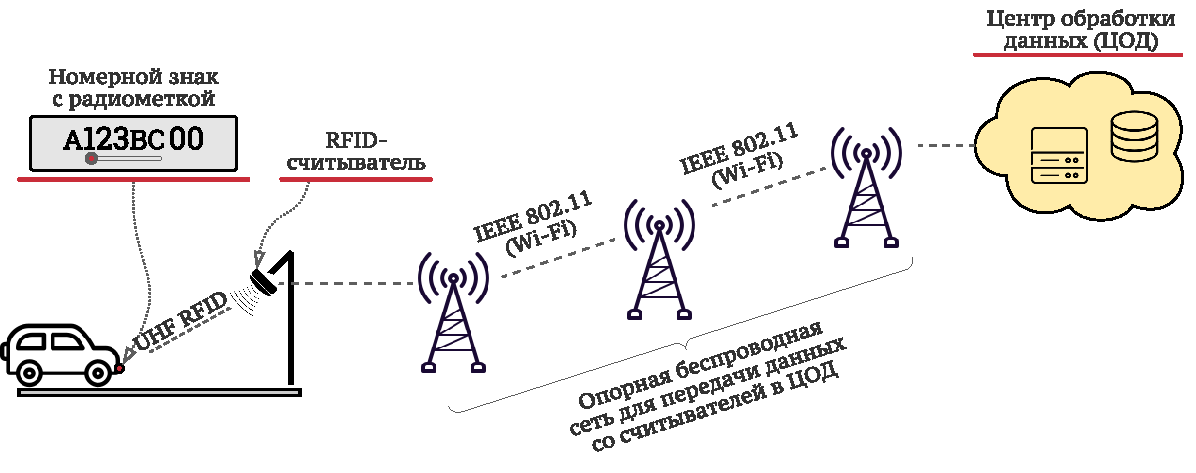
\includegraphics [scale=0.6] {chapter1/ch1_system_overview}
	\caption{Схема распределённой системы радиочастотной идентификации транспорта.}
	\label{fig:ch1_system_overview}
\end{figure}

Основными компонентами простейщей распределенной системы радиочастотной идентификации транспорта являются RFID-метки, RFID-считыватели, телекоммуникационная сеть и центр обработки данных. \textbf{RFID-метки} или \textbf{транспондеры} "--- это устройства, которыми оснащаются транспортные средства. Их назначение "--- передача записанного идентификатора считывателям. В зависимости от используемой технологии, могут быть активными или пассивными, то есть иметь или нет свой источник питания. Подробнее принцип работы меток стандарта EPC Class 1 Gen. 2 (ISO 18000-6C) описан в разделе~\ref{sec:ch1_rfid}. \textbf{RFID-считыватели} "--- активные устройства, осуществляющие чтение идентификаторов меток и их передачу в центр обработки данных. \textbf{Телекоммуникационная сеть} используется для передачи данных о метках от считывателей в центр обработки данных, а также для доступа администраторов к считывателям для их настройки, обслуживания и мониторинга. \textbf{Центр обработки данных} включает информационную систему, в которой собираются данные о прочитанных метках и состоянии работы считывателей.

В качестве примера можно привести системы для бесконтактного сбора оплаты проезда на автодорогах, например "--- на участках трасс М-4 <<Дон>>, М-1 <<Беларусь>> и Центральной кольцевой автодороге (ЦКАД). В некоторых странах (например, в Чили, ЮАР, Азербайджане) проводились эксперименты по более масштабному внедрению RFID, для регистрации всех или определенной группы автомобилей. Подобный эксперимент проводился и в России, в республике Татарстан, его результаты будут более подробно рассмотрены в настоящей работе.

Для получения данных о проезжающем транспортном средстве оно должно быть оснащено одной или несколькими RFID-метками, причем выбранная технология радиочастотной идентификации должна обеспечивать чтение метки на расстоянии 10--20 метров. Одной из наиболее подходящих технологий RFID, отвечающих этому требованию, является СВЧ-RFID стандарта EPC Class 1 Generation 2~\cite{StdGen2}, работающая в диапазоне 860--920 МГц. В частности, эта технология была использована в эксперименте, проведенном в городе Казань. В качестве альтернативы также можно использовать активные метки, или технологию DSRC, которая используется на уже упомянутых платных дорогах М-1, М-4 и ЦКАД.

%\subtodo{Добавить ссылки на DSRC и активные RFID}

Для передачи информации о считанных метках RFID-считыватели должны быть подключены к центрам обработки данных. Возможны три пути решения этой задачи: подключение к существующей проводной или беспроводной сети, коммутационное оборудование которой находится вблизи точек размещения считывателей; использование сотовой сети; построение отдельной сети для подключения считывателей. Использование существующих сетей оказывается не всегда возможным, особенно при развертывании системы за пределами крупных населённых пунктов. Кроме того, сети могут быть перегружены (например, если они уже используются для передачи данных с городских камер видеонаблюдения). Из-за ограниченности покрытия использование сотовой сети также не всегда возможно. В качестве примера, в настоящем исследовании будем рассматривать построение отдельной беспроводной сети. Как будет показано, для работы системы не нужно высокоскоростных каналов, и для подключения большого количества считывателей (порядка нескольких сотен) достаточно многошаговой сети, построенной на основе технологии IEEE 802.11g, оборудование которой очень недорогое и позволяет строить беспроводные соединения на расстояниях до нескольких десятков километров.

В центре обработки данных должна собираться как информация о зарегистрированных считывателями метках, так и о состоянии работы оборудования. Если в состав системы входят камеры, радары и прочее оборудование, в информационном центре можно объединять данные, полученные от различных источников. Например, объединяя результаты идентификации номерных знаков по фото с данными, полученными от считывателей, можно существенно повысить достоверность распознавания транспортного средства в условиях плохой видимости. Возможна интеграция и с системами приема оплаты или с базами розыска угнанных машин.

\begin{table}[ht!]
    \renewcommand{\arraystretch}{1.3}
    \caption{Технологии, используемые в распределённой системе радиочастотной идентификации транспорта, разработанной в рамках диссертационной работы.}
    \label{table:ch1_technologies}
	\begin{tabular}{ |p{0.17\linewidth}|p{0.26\linewidth}|p{0.47\linewidth}| }\hline
		Компонент & Технология & Комментарии\\\hline\hline
		Метки & EPC Class 1 Gen. 2 & Пассивные метки в номерных знаках или на стикерах под лобовым стеклом.\\\hline
		Считыватели & EPC Class 1 Gen. 2 & RFID-считыватели устанавливаются над дорогой, поддерживают до четырх антенн и подключаются к сети.\\\hline
		Сеть & IEEE 802.11 & Многошаговая беспроводная сеть с каналами, в которых используется схема доступа CSMA/CA.\\\hline
		ЦОД &  & Различное программное обеспечение для получения, сохранения и анализа данных о метках.\\\hline
	\end{tabular}
\end{table}

В ходе исследования, результаты которого приводятся в настоящей диссертационной работе, предполагалось, что для реализации распределённой системы радиочастотной идентификации транспорта используются технологии, описанные в табл.~\ref{table:ch1_technologies}.


% Следует оговориться, что в современных беспроводных сетях IEEE 802.11 используются гораздо более сложные и эффективные механизмы, нежели DCF, описываемый и исследуемый в настоящей работе; вместе с тем, механизм DCF гораздо проще для исследования, и, как будет показано в последующих главах, его вполне достаточно для эффективной реализации системы передачи данных со многих считывателей, что, вместе с низкой ценой соответствующего оборудования, делает его выбор вполне обоснованным для практической реализации.

% Технология радиочастотной идентификации далее рассматривается гораздо подробнее, чем протоколы передачи данных по беспроводным каналам. Это связано с тем, что вероятность идентификации движущихся меток, которая исследуется в следующих главах, существенно зависит от множества параметров протокола EPC Class 1 Generation 2. В то же время, при исследовании задержек в передаче данных по беспроводным каналам нас главным образом будет интересовать длительность обслуживания, в корректном моделировании которой заключается основная сложность работы, поэтому при описании протокола IEEEE 802.11 DCF мы сделаем акцент именно на временных аспектах работы и на механизме борьбы с коллизиями, игнорируя особенности кодирования и модуляции, а также прочие части протокола.




%%%%%%%%%%%%%%%%%%%%%%%%%%%%%%%%%%%%%%%%%%%%%%%%%%%%%%%%%%%%%%%%%%%%%%%%%%%%%%%%
\section{Постановка задач исследования}\label{sec:ch1_problems}
%%%%%%%%%%%%%%%%%%%%%%%%%%%%%%%%%%%%%%%%%%%%%%%%%%%%%%%%%%%%%%%%%%%%%%%%%%%%%%%%

При проектировании и построении распределённой системы радиочастотной идентификации транспорта возникает целый ряд задач, относящихся как непосредственно к идентификации транспорта, так и к организации связи между считывателями и центром обработки данных. Рассмотрим подробнее задачи, решению которых посвящена диссертационная работа.

%%% --------------------------------------------
\subsection{Исследование эффективности радиочастотной идентификации мобильных меток}
%%% --------------------------------------------

Критерием работоспособности системы является процент успешно распознанных транспортных средств. Задача осложняется тем, что метки могут двигаться с высокой скоростью (порядка 100--150~км/ч), а время, доступное для их чтения, крайне ограничено, так как считыватель может получить данные от метки лишь на небольшом расстоянии, порядка десяти метров. При различных настройках протокола EPC Class 1 Gen. 2 скорость обмена данными с меткой и вероятность успешной передачи сообщений могут меняться в очень широких пределах. Дополнительную сложность задаче придают многолучевое распространения сигналов между считывателем и меткой (как минимум, присутствие отраженного от дороги луча), наличие эффекта Доплера, а также использование метода обратного рассеяния для передачи ответов меток. Для решения задачи оценки работы системы радиочастотной идентификации удобно использовать методы имитационного моделирования, позволяющие учесть как параметры протокола, так и особенности распространения сигналов.

Отдельные аспекты работы считывателей можно исследовать с помощью методов теории случайных процессов. Хотя такой подход затрудняет учет всего объема факторов, влияющих на производительность системы, он позволяет более детально изучить отдельные закономерности, в частности "--- влияние периодических отключений питания и изменений подмножеств опрашиваемых меток на вероятность успешной идентификации. Для построения аналитической модели протокола нужно формально описать компоненты, определяющие состояние системы, а также формализовать операции, которые считыватель может осуществлять над метками. После этого можно исследовать свойства этих операций и найти способы получения оценки успешного чтения меток.

Таким образом, для исследования эффективности системы радиочастотной идентификации автомобилей нужно решить следующие задачи:

\begin{enumerate}
    \item Выявить факторы, влияющие на вероятность успешной идентификации мобильной RFID-метки.
    \item Построить формальную математическую модель системы радиочастотной идентификации, исследовать свойства операций, осуществляемых считывателем над множеством мобильных меток.
    \item Разработать аналитические и имитаицонные модели для получения оценки вероятности идентификации мобильных RFID-меток.
    \item Определить параметры протокола и настройки считывателей, при которых доля успешно идентифицированных автомобилей с RFID-метками оказывается не ниже 90\%.
\end{enumerate}

Решению этих задач посвящены главы 2 и 3 диссертации.



%%% --------------------------------------------
\subsection{Анализ производительности опорной сети}
%%% --------------------------------------------

Для работы некоторых приложений важно обеспечить быструю передачу информации о прочитанных метках в центр обработки данных. Например, это необходимо для реализации бесконтактной оплаты проезда или для поиска угнанных транспортных средств. Для анализа межконцевых задержек можно использовать как имитационное моделирование, так и аналитические модели, построенные на базе теории массового обслуживания.

Модели открытых тандемных сетей массового обслуживания хорошо известны и исследованы. Основная сложность их применения к задаче поиска межконецвых задержек пакетов, передаваемых в многошаговых сетях, заключается в выборе адекватных распределений интервалов между поступлениями пакетов в сеть и распределений длительности передачи пакетов по каналам связи.

В диссертационном исследовании предполагается, что опорная сеть строится на базе беспроводных линий связи с каналами CSMA/CA. Для моделирования каналов связи используются системы массового обслуживания $MAP/PH/1/N$, в которых интервалы между поступлениями пакетов в сеть моделируются марковскими случайными потоками (MAP), время обслуживания пакетов имеет распределение фазового типа (PH), а размер очереди ограничен. Получение численных характеристик открытых сетей $MAP/PH/1/N \rightarrow \bullet/PH/1/N \rightarrow \dots \rightarrow \bullet/PH/1/N$ осложняется экспоненциальным ростом пространства состояний при увеличении числа узлов в сети, и отдельной задачей является поиск эффективных способов получения численных оценок таких сетей.

Для оценки производительности опорной сети в диссертации решаются следующие задачи:

\begin{enumerate}
    \item Поиск PH-распределений, адекватно моделирующих время обслуживания в беспроводных сетях с каналами CSMA/CA.
    \item Оценка возможности использования методов редукции пространства состояний для получения численных оценок межконцевых задержек в открытых тандемных сетях массового обслуживания с узлами типа $MAP/PH/1/N$.
    \item Получение численных оценок межконецвых задержек для многошаговой беспроводной сети с помощью аналитического и имитационного моделирования.
    \item Оценка максимального количества считывателей, одновременно использующих беспроводную опорную сеть, с помощью имитационного и стендового моделирования.
\end{enumerate}

Решению этих задач посвящена глава 4 диссертации.


%%% --------------------------------------------
\subsection{Экспериментальная реализация системы}
%%% --------------------------------------------

Для того, чтобы исследовать работоспособность системы радиочастотной идентификации автомобилей, были разработаны экспериментальные RFID-считыватели, распределенная система управления считывателями и программное обеспечение для центров обработки данных. Разработанный программно-аппаратный комплекс проходил испытания в трех экспериментах. Первый эксперимент прошел в 2014--2015 годах в городе Казань. Тогда метками были оснащены около 750 автобусов, в двух точках города установлены RFID-считыватели, информация с которых передавалась в центр обработки данных в ГИБДД. За несколько зимних месяцев была собрана статистика, вероятность идентификации составила 92--95~\%. Следующий эксперимент проходил в 2020 году также в Казани, его целью была проверка системы при идентификации автомобилей, движущихся со скоростями до 170~км/ч и совершающих различные маневры. Третий эксперимент начался летом 2021 года на ЦКАД, его целью была проверка применимости системы для сбора данных для оплаты проезда. Все эксперименты завершились успешно.

При разработке программного обеспечения RFID-считывателей требовалось обеспечить его высокую надежность, быстродействие, а также гибкость. В частности, было принято решение разделить потоки данных и управления (сигнализации) так, чтобы, с одной стороны, сделать невозможным изменение параметров работы считывателя каким-либо образом, кроме как через административный интерфейс, а с другой стороны "--- упростить подключение внешних клиентов для получения потоков считанных меток. Программное обеспечение было спроектировано таким образом, чтобы можно было в быстро заменить радиомодули RFID-считывателей без изменения кода остальных компонентов, а также обеспечить возможность выноса части компонентов за пределы считывателя.

В состав разработанного программного обеспечения входит управляющий модуль (супервайзер), адаптеры радиомодулей, интерфейсы управления (веб-интерфейс, интерфейс командной строки), а также модули для приема и обработки потоков данных о прочитанных метках. Все программное обеспечение, за исключением веб-интерфейса, было реализовано на языках C и C++.

Для экспериментального исследования производительности системы радиочастотной идентификации были решены следующие задачи:

\begin{enumerate}
	\item Разработка архитектуры распределённой системы управления RFID-считывателями и протоколов связи между компонентами системы.
	\item Программная реализация распределённой системы управления и разработка программного обеспечения для приема, обработки и записи данных о прочитанных метках.
	\item Проведение экспериментальных исследований и получение оценки вероятности успешной идентификации автомобилей при различных скоростях движения, маневрах, погодных условиях.
\end{enumerate}

Решению этих задач посвящена глава 5 диссертации.



%%%%%%%%%%%%%%%%%%%%%%%%%%%%%%%%%%%%%%%%%%%%%%%%%%%%%%%%%%%%%%%%%%%%%%%%%%%%%%%%
\section{Радиочастотная идентификация транспортных средств}\label{sec:ch1_rfid}
%%%%%%%%%%%%%%%%%%%%%%%%%%%%%%%%%%%%%%%%%%%%%%%%%%%%%%%%%%%%%%%%%%%%%%%%%%%%%%%%

Технология радиочастотной идентификации (RFID) является альтернативой для традиционной идентификации номеров транспортных средств по фото. Для использования этой технологии автомобили оснащаются радиометками, а в точках контроля размещаются считыватели. Когда метка проезжает мимо считывателя, она передает свой идентификатор, по которому определяется номер автомобиля. К преимуществам этой технологии относится относительно низкая стоимость оборудования, низкие требования к пропускной способности каналов связи, отсутствие необходимости в частом обслуживании и слабая зависимость от погодных условий.

Существует несколько различных технологий радиочастотной идентификации. В \textbf{активных} системах используются метки, обладающие собственным источником питания. Часто такие системы работают в диапазоне 2.4 ГГц и могут быть основаны, например, на технологиях IEEE 802.11 (WiFi) или ZigBee. Можно выделить технологию DSRC (Dedicated Short-Range Communication), которая часто используется в системах оплаты проезда по автомагистралям, в том числе и в России. Дальность действия считывателя в системах с активными метками может достигать десятков или даже сотен метров, но метки достаточно громоздки и дорогостоящи.

К другому классу относятся \textbf{пассивные} системы, в которых метки не обладают собственными источниками энергии. Для работы и передачи данных метки в таких системах используют энергию, получаемую из электромагнитного поля, создаваемого считывателем. RFID-системы LF-диапазона (125 "--- 134 кГц, ISO/IEC 18000-2) характеризуются малым расстоянием идентификации (порядка нескольких сантиметров) и используются, например, для чипирования животных. Системы HF-диапазона (13,56 МГц, стандарты ISO/IEC 18000-3, ISO/IEC 15693, ISO/IEC 14443 A,B) очень широко распространены в области электронной оплаты (например, оплата проезда на общественном транспорте) и контроля доступа, характеризуются низкой стоимостью и дальностью порядка нескольких миллиметров или сантиметров. Системы UHF-диапазона (860 "--- 960 МГц, ISO/IEC 18000-6C, EPC Gen-2) работают на расстояниях до 15--20 метров и используются в логистике, торговле, контроле доступа и на производствах. Кроме того, метки UHF-диапазона иногда оснащаются собственным источником питания, который может использоваться для работы встроенного сенсора. В этом случае метка может передавать результаты измерений, полученные от сенсора, а питание также может использоваться для усиления отражаемых сигналов. Такие метки называются полупассивными или полуактивными.


%%% --------------------------------------------
\subsection{Стандарт EPC Class 1 Generation 2}\label{sec:ch1_rfid_std}
%%% --------------------------------------------

Стандарт EPC Class 1 Generation 2~\cite{StdGen2} (ISO/IEC 18000-6C, ГОСТ Р 58701-2019 \cite{GostRfid}) описывает физический (PHY) и канальный (MAC) уровни системы радиочастотной идентификации пассивных и полупассивных меток. На физическом уровне стандарт описывает способы модуляции и кодирования сигналов, а на канальном уровне "--- протокол обмена данными между считывателем и метками. Протокол основан на Slotted ALOHA \cite{Abramson1970, Roberts1975}, позволяет бороться с коллизиями при нахождении нескольких меток в зоне считывателя, а также содержит средства для чтения и записи данных на метки.

Поскольку пассивные метки не имеют собственного источника питания, счиытватель постоянно создает электромагнитное поле, которое используется метками для получения энергии. Периодически считыватель отключает питание, обеспечивая меткам возможность сбросить некоторые регистры и флаги. В то время, когда считыватель не осуществляет передачу своих команд, он генерирует синусоидальный сигнал (Constant Wave, CW), который метки используют в качестве несущей "--- для передачи ответов метки модулируют отражаемый ими сигнал CW, полученный от считывателя, изменением своего коэффициента отражения (т.е. передача данных от меток ведётся методом обратного рассеяния).

Метки не могут сами инициировать обмен данными со считывателем, они всегда передают свои сообщения в ответ на получаемые от считывателя команды. Стандарт допускает следующие основные действия с меткой: инвентаризацию, чтение, запись и блокирование памяти, а также уничтожение метки. Инвентаризация "--- это опрос меток, в ходе которого они передают считывателю свои идентификаторы EPCID и выполняют другие операции, которые может запросить считыватель.  Блокирование памяти означает, что считыватель впоследствии не сможет записать эту область памяти. Наконец, операция уничтожения метки приводит к тому, что в будущем метка никогда не будет участвовать в инвентаризации. Протокол определяет и другие операции, включая средства для защиты доступа к данным. Производители могут реализовать дополнительные операции на своих метках. В рамках диссертационной работы интерес будут представлять только инвентаризация и чтение памяти.


%%% ~~~~~~~~~~~
\subsubsection{Логическая структура памяти метки}\label{sec:ch1_rfid_std_memory}
%%% ~~~~~~~~~~~

Каждая метка включает в себя четыре банка памяти (см. рис. \ref{fig:ch1_banks}): EPC, TID, зарезервированную память (Reserved) и пользовательскую память (User).

\begin{figure}[ht]
  \centering
  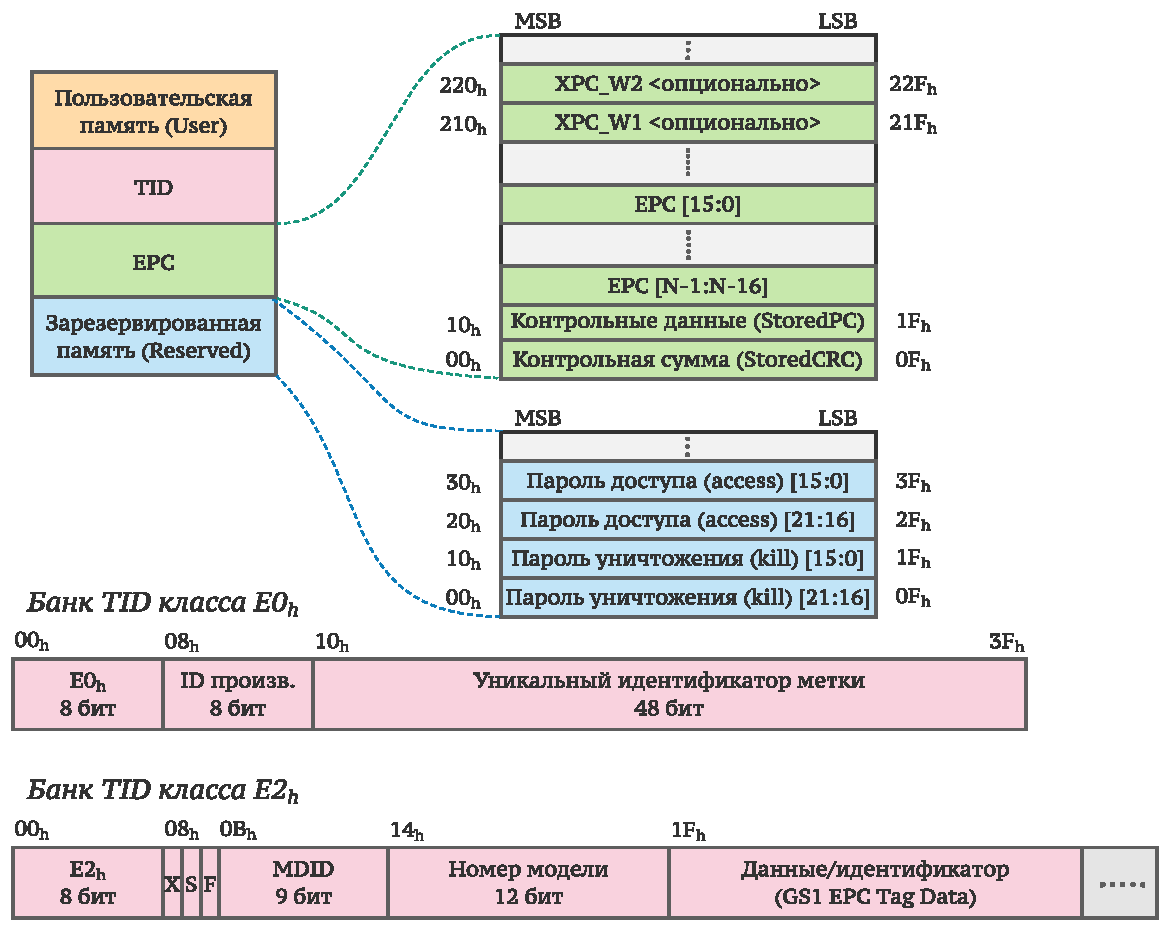
\includegraphics [scale=0.8] {chapter1/ch1_banks}
  \caption{Логическая структура памяти метки}
  \label{fig:ch1_banks}
\end{figure}

Банк EPC содержит код EPC (Electronic Product Code), контрольную сумму (StoredCRC) и служебную информацию (PC, Protocol Control), в которой хранятся данные о длине поля EPC, доступности пользовательской памяти и прочую информацию. Объем памяти в поле EPC может меняться от метки к метке, распространненым значением является 96 бит. Чтобы не путать название банка памяти и значение EPC, значение в дальнейшем будем называть EPCID.

Банк Reserved хранит пароли для блокирования и уничтожения меток, если метка поддерживает соответствующие операции.

Банк TID хранит данные о производителе и модели метки, а также ее уникальный идентификатор. Главная особенность банка TID "--- фабричная защита от изменений значения, записанного при производстве метки, поэтому его удобно использовать в задаче надежной идентификации объектов. Первые 8 бит TID содержат идентификатор класса, который может быть равен либо $\text{E0}_\text{h}$, либо $\text{E2}_\text{h}$. Если идентификатор класса равен $\text{E0}_\text{h}$, то длина банка равна 64 битам, второй октет содержит идентификатор производителя, а последние 48 бит содержат серийный номер метки. Такие метки производства NXP использовались в эксперименте в Казани в 2014 году. Структура банка TID для класса $\text{E2}_\text{h}$ более сложная, а его размер "--- больше. Следюущие после первого октета три бита "--- служебные флаги, после них "--- 9-битный идентификатор производителя MDID (Mask Designer Identifier), далее 12-битный номер модели и уже после него уникальный номер метки. Например, метки производства АО <<Микрон>>, которые использовались в экспериментах 2020-го и 2021-го года, имеют класс $\text{E2}_\text{h}$ и содержат 96-битные значения.

Банк пользовательской памяти может иметь достаточно большой объем (порядка 512 бит) и используется для хранения дополнительных данных, например "--- подробной информации о маркированном предмете.


%%% ~~~~~~~~~~~
\subsubsection{Физический уровень}\label{sec:ch1_rfid_std_phy}
%%% ~~~~~~~~~~~

При передаче данных от считывателя к меткам используется амплитудную модуляцию DSB-ASK, SSB-ASK или PR-ASK. Для кодирования используется схема PIE (Pulse Interval Encoding), в которой нули и единицы кодируются символами data-0 и data-1 различной длины (см. рис.~\ref{fig:ch1_pie}).

\begin{figure}[ht]
  \centering
  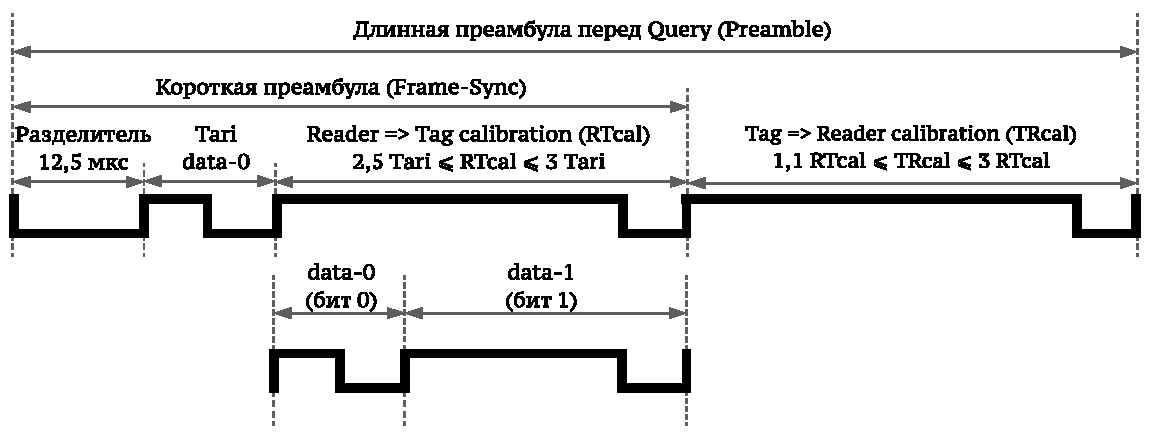
\includegraphics [scale=0.8] {chapter1/ch1_pie}
  \caption{Символы в схеме PIE и преамбулы команд RFID-считывателя}
  \label{fig:ch1_pie}
\end{figure}

Передачу каждой команды считыватель начинает с синхронизирующей последовательности (преамбулы). Стандарт определяет два вида преамбул (см. рис.~\ref{fig:ch1_pie}): длинную, называемую в стандарте преамбулой, и короткую, называемую синхронизацией кадра, (Frame-Sync). Оба вида преамбул начинаются с постоянного разделителя длительностью 12,5~мкс, за ним идут символы ноль (data-0) и RTcal (Reader-to-Tag calibration). Длительность символа data-0 называется Tari. Длительность символа RTcal равна суммарной длительности нуля и единицы, этот символ используется меткой для различения символов data-0 и data-1: если символ короче половины RTcal, то это ноль, иначе "--- единица. Короткая преамбула завершается передачей RTcal, а длинная содержит также символ TRcal (Tag-to-Reader calibration), длительность которого используется меткой для расчета скорости, с которой она должна передавать свой ответ.

Длинная преамбула отличается от короткой наличием символа TRcal и передается перед первой командой Query, с которой считыватель начинает опрос меток. Так как метка, не получившая Query, все равно не сможет участвовать в опросе, передавать TRcal в последующих кадрах не имеет смысла и используется короткая преамбула, содержащая только ту информацию, которая нужна метке для успешного декодирования команды.

Отметим, что из-за использования PIE длительность кадров, передаваемых считывателем, зависит от числа нулей и единиц в команде. Поэтому для точного моделирования протокола необходимо учитывать результат кодирования команд.

Метка передает свой ответ, модулируя несущую, полученную от считывателя. Метка может использовать амплитудную (ASK) или фазовую (PSK) модуляцию. В качестве схемы кодирования используется либо код FM0, либо коды Миллера с 2, 4 или 8 символами на бит. Все схемы кодирования, поддерживаемые метками, имеют память, то есть вид символа, кодирующего следующий бит, определяется предыдущим битом. Перед передачей ответа метка передаёт преамбулу, которая может быть обычной или расширенной. Короткая преамбула равна по длительности 6 битам для кода FM0 и 10 битам для кодов Миллера, а расширенная - 18 и 22 битам соответственно. Кроме того, после каждого ответа метки следует символ, не кодирующий ни ноль, ни единицу.

Для вычисления скорости передачи символов метка вычисляет величину BLF (Backscatter Link Frequency) по следующей формуле:

$$
\text{BLF} = \frac{\text{DR}}{\text{TRcal}},
$$
где DR (Divide Ratio) - величина, передаваемая в команде Query, и принимающая одно из двух значений: 8 или 64/3. Для вычисления битовой скорости необходимо разделить BLF на число символов на бит в используемом меткой методе кодирования (M=1,2,4,8). В отличие от считывателей, использующих PIE, все биты в ответах меток имеют одинаковую длительность, поэтому их содержание не оказывает влияния на длительность передачи ответов.



%%% ~~~~~~~~~~~
\subsubsection{Логический уровень}\label{sec:ch1_rfid_std_logic}
%%% ~~~~~~~~~~~

Протокол доступа к каналу, описываемый в стандарте \cite{StdGen2}, основан на протоколе Framed Slotted ALOHA \cite{Roberts1975, Abramson1970}. Все время работы разбито на \textbf{раунды} (см. рис. \ref{fig:ch1_inventory}), которые начинаются передачей считывателем команды Query. Эта команда, среди прочего, несет в себе параметр Q, который используется метками для расчета количества слотов в раунде как $2^\text{Q}$. Получив Query, метка выбирает случайный номер слота \textit{SN} для передачи своего ответа от 0 до $2^\text{Q}-1$. При последующем получении команд QueryRep метка уменьшает значение счетчика \textit{SN}. Когда счетчик доходит до 0, метка генерирует и передает случайное 16-битное число (RN16). Считыватель, получив это случайное число, пересылает его в команде Ack. Метка сравнивает полученное значение с отправленным. Если значения совпадают, то в ответ на Ack метка пересылает свой EPCID с контрольной суммой (PacketCRC) и контрольными данными (PC). Если же значения не совпадают, метка считает, что Ack предназначен не ей, и ничего не отвечает.

\begin{figure}[ht]
  \centering
   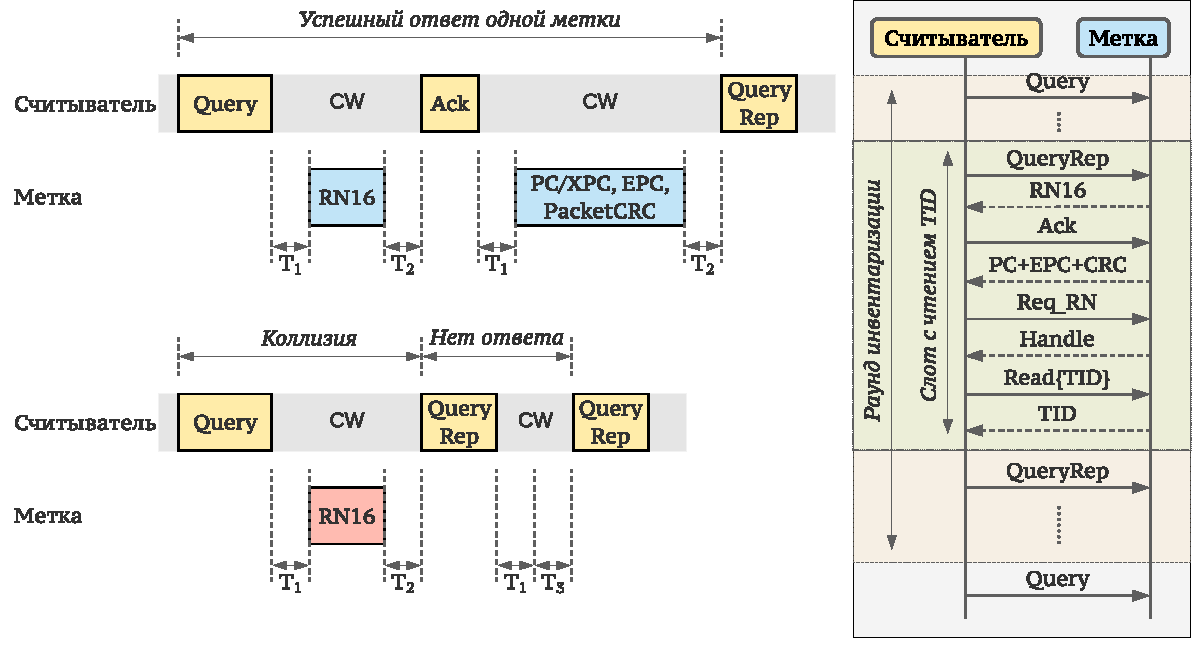
\includegraphics [scale=0.8] {chapter1/ch1_inventory}
  \caption{Схема опроса меток и раунд инвентаризации}
  \label{fig:ch1_inventory}
\end{figure}

Стандарт определяет границы интервалов, которые должны пройти между последовательными командами и ответами:

\begin{itemize}
	\item $T_1$: минимальное время между концом последнего символа команды и первым символом преамбулы ответа;
	\item $T_2$: минимальное время между окончанием последнего (псевдо-) бита ответа метки и первым символом преамбулы команды считывателя;
	\item $T_3$: минимальный интервал между окончанием $T_1$ и следующей командой считывателя.
\end{itemize}

Все, что происходит от передачи QueryRep до получения ответа от метки с EPCID, называется \textit{стадией инвентаризации}. Именно в ней разрешаются коллизии "--- если несколько меток выбрали один слот и одновременно передали слова RN16, то считыватель, скорее всего, не сможет получить ни одно из них и либо вовсе не отправит Ack, либо отправит Ack с неправильным значением. Если же метка получила Ack с правильным значением, то коллизии не было, поэтому она может передать более длинное (по сравнению с RN16) значение EPCID. Если считыватель смог обнаружить ошибку в ответе метки, он может передать команду NACK, получив которую метка сможет определить, что ее идентификатор не был успешно передан. Также считыватель может повторно отправить Ack, чтобы метка повторила передачу EPCID.

Если после получения EPCID считывателю нужно выполнить над меткой другие действия, он начинает \textit{стадию доступа}. В ней он запрашивает новое случайное число от метки с помощью команды Req\_RN и, после получения ответа, передает команду чтения, записи, блокирования или уничтожения метки. Если метка использует пароль для доступа, то перед передачей команды считыватель должен отправить пароль.

Помимо стадий инвентаризации и доступа, стандарт определяет \textit{стадию выбора}. До отправки команды Query считыватель может передать команду Select, в которой задать параметры тех меток, ответы от которых он хочет получить в текущем раунде. Эту команду удобно использовать при опросе большого числа меток, например на складе. Еще одна интересная особенность стандарта "--- возможность динамически изменять число слотов. Если считыватель обнаруживает, что коллизии происходят слишком часто или, наоборот, слишком много пустых слотов, он может передать команду QueryAdjust с новым значением Q и запросить метки, которые еще не ответили в этом раунде, выбрать новые слоты. Подробнее про протокол взаимодействия между считывателями и метками можно прочитать в стандарте~\cite{StdGen2}.

В диссертационной работе будет использоваться фиксированное значение Q и только одна операция доступа "--- чтение банка TID. Для ее выполнения считыватель использует команду Read, в которой отмечает нужный банк (TID), адрес начала памяти ($\text{00}_\text{h}$) и число 16-битных слов, которые нужно прочитать. Если команда выполнена успешно, метка передает в ответ хранящееся значение. Пример чтения банка TID показан на рис.~\ref{fig:ch1_inventory}.



%%% ~~~~~~~~~~~
\subsubsection{Сессии}\label{sec:ch1_rfid_std_sessions}
%%% ~~~~~~~~~~~

Сессии позволяют разграничить множество окружающих считыватель меток. Каждая метка должна поддерживать четыре сессии S0, S1, S2 и S3. Для каждой сессии метка имеет отдельный флаг, значения которого в стандарте обозначаются как $A$ и $B$.

В команде Query считыватель указывает, с какой сессией работает в этом раунде, и какое значение флага сессии должно быть у меток, которые могут участвовать в опросе. После передачи EPCID метка, получив команду Query, QueryRep или QueryAdjust, должна инвертировать хранящееся у нее значение флага ($A \rightarrow B$, $B \rightarrow A$). Если в следующем раунде опрос будет проходить по той же сессии и тому же значению флага, эта метка участвовать в раунде не будет, так как у нее хранится инвертированное значение флага. Если считыватель не смог получить EPCID, он может передать команду NAK "--- в этом случае метка не изменит флаг и сможет участвовать в следующем раунде.

Сессии различаются по требованиям ко времени сохранения значения флага при потере питания, а также к начальным значениям флагов. Флаг сессии S0 всегда инициализируется в значение $A$. Он сбрасывается всякий раз, когда метка теряет питание. Флаг сессии S1 сбрасывается в значение $A$ при включении метки, если со времени его изменения прошло не менее интервала, значение которого может варьироваться от 0,5 с до 5~с. Значение также сбрасывается в том случае, если метка не выключалась и с момента последнего изменения прошло слишком много времени. Флаги сессий S2 и S3 должны сбрасываться в $A$, если с момента выключения метки прошло не менее 2~с. Таким образом, использование сессий S2 и S3 может предотвратить изменение флага в случае краткосрочной потери меткой энергии.

Как будет подробно исследовано в главе 3, выбор сессии и сценария опроса (всегда ли опрашивать метки по значению флага $A$ или чередовать опросы по $A$ и по $B$) оказывает существенное влияние на вероятность успешной идентификации метки.



%%% --------------------------------------------
\subsection{Обзор исследований производительности UHF RFID}\label{sec:ch1_rfid_observe}
%%% --------------------------------------------

Технология радиочастотной идентификации \cite{Finkenzeller2010, Dobkin2008} используется во множестве приложений, от учета товаров на складах, до поиска автомобилей на парковке с помощью дронов \cite{Wu2019}, позиционирования мобильных объектов \cite{Cho2013, Park2013, Errington2010}, расчета скорости движущихся автомобилей \cite{Zhai2018, Choy2020, Jing2013}, и даже выявления признаков усталости водителя \cite{Yang2020} (в последнем случае метки предлагается размещать с двух сторон на шапке), или оперативного поиска потервшихся в городе людей (например, с болезнью Альцгеймера или иными расстройствами) с помощью RFID-считывателей на припаркованных автомобилях \cite{Griggs2018}.

Задача идентификации транспорта является одним из основных применений RFID \cite{StdRainEviWhitepaper}. Первые системы сбора платы за проезд, использующие RFID, появились в США в 1991 году \cite{Landt2005}. Использование RFID для идентификации автомобильного и железнодорожного транспорта исследовалось в работах \cite{Gonzalez2013, Blythe1999, Khan2011, Yoon2008, Al-Naima2011, Tseng2007, Kostrominov2020, Unterhuber2019, Unterhuber2020, Unterhuber2019, Pawowicz2020, Choy2020, Jo2009, Zhang2010, MenesesGonzalez2011, Lonkar2018, Balbin2017, Bhavke2017, Zhang2011, Zhang2010a, Pandit2009, Sundar2015}. В частности, в работе \cite{Unterhuber2020} Unterhuber и соавторы рассматривают систему идентификации быстрого транспорта (автомобилей и поездов) и утверждают, что наиболее критичный параметр, определяющий вероятность идентификации "--- число раундов, в которых успевает принять участие метка. Авторы предлагают простую модель для оценки максимального числа раундов, используют реалистичные модели антенных систем и получают результаты, доказывающие, что UHF RFID можно применять для идентификации очень быстро движущихся автомобилей и поездов. Unterhuber и соавторы также отмечают, что из-за многолучевого распространения и эффекта Доплера может существовать несколько отрезков, на которых возможна идентификация (аналогичные данные получены в моделях, представленных в диссертации). Вместе с тем, в работе \cite{Unterhuber2020} не рассматриваются коллизии или идентификация меток по TID. Стоит также выделить предыдущую работу Unterhuber и соавторов \cite{Unterhuber2019} и работу Marais и соавторов \cite{Marais2013}, в которых представлен анализ оптимального угла наклона антенн при идентификации транспорта.

Использование RFID в рамках интеллектуальных транспортных систем и <<умных городов>> "--- одно из перспективных направлений исследований \cite{Pawowicz2020, Pandit2009, Sundar2015}. Например, Pawłowicz и соавторы в работе \cite{Pawowicz2020} рассматривают задачу идентификации транспортного потока в контексте концепции <<умного города>>, предлагают очень простую аналитическую модель и сравнивают данные, полученные с ее помощью, с результатами макетного моделирования.

Процесс чтения движущихся меток, в общем случае, не является надежным "--- метка может быть потеряна из-за высокой скорости движения, слабого сигнала или коллизий. Для того, чтобы предсказать, будет ли идентифицирована метка, и извлечь дополнительную информацию из данных, полученных от считывателя, можно использовать методы машинного обучения. В работе \cite{Jo2009} Jo и соавторы используют метод опорных векторов (SVM) для предсказания того, будет ли идентифицирован движущийся объект, в зависимости от скорости, угла наклона антенны и положения метки. А в работе \cite{Choy2020} Choy и соавторы используют искусственные нейронные сети для вычисления скорости движения автомобилей по мощности принятого RFID-считывателем сигнала. В работе также отмечено, что основная задача "--- борьба с нарушениями скоростного режима, а метки желательно размещать в номерах автомобилей.

Применение пассивных и активных RFID-тенхологий на дорогах не ограничивается простой идентификацией транспорта. Так, в работах \cite{GarciaOya2018, Jing2016, Hidalgo2013, Jing2013, Cheng2012, Perez2010} предлагается использовать RFID для чтения данных с дорожных знаков или с дорожного полотна. В этом случае метки располагаются на статичных объектах, а считыватели "--- в автомобилях. А в работе \cite{Porter2008} Porter и Kim описывают результаты эксперимента, проведенного в штате Орегон (США), в ходе которого RFID-метки использовались для сбора и передачи данных о пройденным автомобилем пути для дальнейшего расчета налога на топливо при заправке "--- авторы совместно с управлением транспорта штата Орегон исследовали возможность гибкого расчета топливного сбора на основе пройденного автомобилем расстояния. Отметим, что в этой работе использовался RFID в диапазоне 2,4~ГГц с доступом к каналу CSMA/CA. В работах \cite{Zheng2020, HongziZhu2009, Pandit2009} предлагается использовать информацию, полученную при чтении меток, для анализа трафика и траекторий передвижения, позиционирования и поиска угнанных автомобилей. Отметим, что в работе \cite{HongziZhu2009} предполагается использование активных RFID в диапазоне 2,4~ГГц.

Некоторые исследователи предлагают устанавливать пассивные RFID-метки в дорожное покрытие и использовать их для измерения скорости движения или передачи данных автомобилям, оборудованным RFID-считывателем. Cheng и соавторы \cite{Cheng2012} предлагают использовать такие дорожные метки для позиционирования автомобилей. Jing и соавторы \cite{Jing2016} также предлагают размещать метки на полосах движения и использовать их не только для передачи статических данных автомобилям (местоположение, направление движения, ограничение скорости и пр.), но и для записи автомобилями данных о текущей обстановке; эти данные затем могут быть получены другими проезжающими автомобилями, как от меток, так и в результате передачи данных по беспроводной сети между машинами. В работе \cite{Jing2013} Jing и соавторы приводят простой расчет минимального расстояния между метками, при котором водители с агрессивной манерой вождения не смогут ускориться и замедлиться так, чтобы их мгновенная скорость существенно превышала ограничение, но средняя скорость оставалась допустимой.

Отметим, что протокол, лежащий в основе канального уровня стандарта EPC Gen-2 \cite{StdGen2} "--- Framed Slotted ALOHA \cite{Abramson1970}. Исходный протокол ALOHA был представлен в работе \cite{Roberts1975}. В этой же работе, на основе предположения о пуассоновском потоке передаваемых пакетов, была получена оценка пиковой пропускной способности сети как $1/(2e) \approx 0,186$. Позднее, в работе \cite{Abramson1970} был описан способ повышения пропускной способности в два раза за счет разбиения времени на слоты (Slotted ALOHA).

Ряд работ посвящен имитационному моделированию систем UHF RFID \cite{Floerkemeier2009, Arnitz2009, Zhang2010, Jing2016}. Так, в работе \cite{Floerkemeier2009} была предложена модель JiST, реализованная на языке Java; в работе описывается дизайн системы моделирования и ее применение. К сожалению, симулятор JiST давно не обновлялся и, судя по всему, в настоящее время практически не используется. В работе \cite{Arnitz2009} сделан фокус на особенности распространения сигналов, моделировании каналов передачи данных и прочих низкоуровневых особенностях RFID-системы, однако практически не учитываются аспекты верхнего (логического) уровня. Авторы работы \cite{Zhang2010} предлагают использовать комбинацию симулятора OMNeT++ для моделирования логики и MATLAB для моделирования физического уровня, в качестве примера рассматривают модель UHF RFID. В работе \cite{Jing2016} также упоминается имитационная модель RFID, разработанная в системе моделирования OMNeT++.

Для того, чтобы адекватно моделировать процесс обмена сообщениями, учитывая потери из-за ненадежности каналов связи между считывателем и меткой, требуется детально учитывать особенности антенных систем, чувствительность меток и считывателя и свойства распространения сигналов. Эти вопросы изучлись во многих работах, в том числе в \cite{Dimitriou2014, Azpilicueta2016,  Griffin2009,  Nikitin2012, Nikitin2009, Nikitin2008, Nikitin2007, Nikitin2006, Nikitin2006a, Rao2005, Zanetti2010}. Работы \cite{Dimitriou2014, Azpilicueta2016} предлагают модели распространения сигналов, основанные на технике трассировки лучей. Авторы работы \cite{Dimitriou2014} рассматривают особенности распространения сигналов внутри помещений со множеством отражений, однако акцентируются на стационарных объектах и игнорируют эффект Доплера. В работе \cite{Azpilicueta2016} авторы моделируют систему с движущимися транспортными средствами, однако не учитывают параметры логического уровня и фокусируются на оценке энергетических параметров в сравнении с данными, полученными из эксперимента. В работах \cite{Nikitin2008, Griffin2009} предложена точная модель для расчёта бюджета соединений. В работе \cite{Nikitin2008} Никитин и Рао рассматривают возможные конфигурации антенн считывателей, приводят типичные значения SNR для различных компонентов антенных систем считывателя, демонстрируют существенные различия в расчете затухания сигнала для однолучевой и многолучевой моделей, приводят формулы для расчета бюджета соединений, а также приводят результаты измерений для различных меток. Кроме того, авторы отмечают, что основной вклад в шум при приеме ответов считывателем вносит не термический шум, а утечка излучаемого сигнала. В диссертационной работе этот факт будет использоваться при расчете SNR.

Влияние коллизий и расчет BER рассматривается в работе Lazaro и соавторов \cite{Lazaro2009}. Авторы предлагают для расчета BER использовать не обычную модель канала с аддитивным Гауссовым шумом (AWGN), а модель, полученную из AWGN усреднением по соотношению SNR, которое предполагается случайным, имеющим распределение Рэлея.

Значительное число работ посвящено анализу производительности систем радиочастотной идентификации. Авторы пользуются эмпирическими методами \cite{Buettner2008}, используют аппарат марковских случайных процессов как с идеальным каналом \cite{Vogt2002, Wang2009, Vahedi2012, Vales-Alonso2009, Vales-Alonso2011, Tong2007, Vales-Alonso2017}, так и с каналом с ошибками \cite{DiMarco2014}, а также используют иные аналитические подходы для анализа производительности \cite{Ahmed2016, Yan2014, Jeon2009, Kim2007}. В ряде работ также сравнивается производительность протокола Frame Slotted ALOHA с альтернативными протоколами и расширениями \cite{Vahedi2014, LaPorta2011}. В работе \cite{Buettner2008} M. Buettner пришел к выводу, среди прочего, что в ряде случаев при опросе выгоднее не пересылать повторно команды ACK при потере ответа от метки, а лучше выключиться и попробовать в следующем раунде или использовать иную стратегию опроса. Аналогичный подход будет использоваться в диссертационном исследовании. Отметим также работу \cite{Vales-Alonso2017}, в которой с помощью дискретной цепи Маркова исследуется эффект потери метками питания. Авторы описывают систему в виде двумерной цепи, моделируя изменение числа меток, которые продолжают участвовать в опросе, и число меток, уже передавших свои данные. В результате проведенного анализа, авторы находят оценки вероятности идентификации к концу раунда опроса и пропускную способность системы. В отличие от представленных в диссертационной работе моделей, потери пакетов возникают только вследствие коллизий, не учитываются сессии, и моделирование производится по слотами в одном раунде, а не по раундам. Также стоит выделить работу \cite{Pawowicz2020}, в которой предлагается очень простая модель для оценки вероятности потери метки, то есть ее проезда области чтения без идентификации. Авторы делят область чтения на сегменты фиксированной длины и, полагая, что передавшие свой идентификактор метки не участвуют в последующих раундах, предлагают простой метод расчета. Как и в главе 3 диссертационного исследования, авторы \cite{Pawowicz2020} рассматривают изменения системы между раундами, в том числе "--- поступления и выходы метки из области чтения. В то же время, степень детализации модели в диссертационном исследовании существенно выше.

Модель системы радиочастотной идентификации транспорта, описанная в главе 2, в значительной степени опирается на результаты, описанные в работах Никитина и Рао \cite{Nikitin2008}, Lazaro \cite{Lazaro2009}, Griffin \cite{Griffin2009} и других. Новизна предложенной в диссертации модели заключается в совместном моделировании как особенностей радиопередачи (включая эффект Доплера и многолучевое распространение), так и антиколлизионного протокола в единой имитационной модели и получении из нее оценок вероятности идентификации автомобилей по паре меток. Кроме того, в большинстве работ не рассматривается идентификация по TID, которая исследуется в диссертационной работе.

Аналитическая модель, описанная в главе 3, также имеет ряд отличий от существующих исследований. Во-первых, переходы марковской цепи происходят на границах раундов, а не слотов, и учитывают сбросы питания и смены флагов опроса меток. Во-вторых, модель учитывает потери произвольных пакетов из-за ненулевой битовой ошибки. В-третьих, модель состоит из двух марковский процессов, первый из которых нужен для расчета числа меток, участвующих в раундах, а второй "--- для оценки вероятности идентификации. В-четвертых, матрицы переходных вероятностей строятся в виде произведения матриц отдельных операций (проведение опроса, инвертирование флага опроса, сброс питания, добавление или удаление метки из области чтения). Из-за этого марковские процессы оказываются неоднородными и тяжелее в анализе, но предложенный метод становится очень гибким. В дальнейшем метод можно расширить на более сложные операции.




%%%%%%%%%%%%%%%%%%%%%%%%%%%%%%%%%%%%%%%%%%%%%%%%%%%%%%%%%%%%%%%%%%%%%%%%%%%%%%%%
\section{Передача данных по беспроводным сетям}\label{sec:ch1_wifi}
%%%%%%%%%%%%%%%%%%%%%%%%%%%%%%%%%%%%%%%%%%%%%%%%%%%%%%%%%%%%%%%%%%%%%%%%%%%%%%%%

Исторически, одним из первых методов доступа к каналу стал CSMA/CA, который был взят за основу уже в первых версиях стандарта IEEE 802.11. Базовый механизм доступа, описанный в этом стандарте и основанный на CSMA/CA, называется DCF (Distributed Coordination Function). Хотя современные версии стандарта используют гораздо более совершенные методы конкурентного доступа, позволяющие учитывать QoS, производить групповые передачи, подтверждать группы пакетов вместо отдельных, объединять каналы и пр., так или иначе в их основе лежит DCF. Ввиду своей простоты, мы будем использовать его в качестве модельного образца конкурентного доступа к каналу.


%%% --------------------------------------------
\subsection{Механизм доступа к каналу IEEE 802.11 DCF}\label{sec:ch1_wifi_dcf}
%%% --------------------------------------------

Метод доступа CSMA/CA и механизм DCF хорошо известны и подробно описаны в различных статьях и книгах (например, см. работу Bianchi~\cite{Bianchi2000}), а наиболее подробное описание можно найти в стандарте IEEE 802.11. Вкратце опишем основы механимза.

Когда станции требуется передать новый пакет, в первую очередь она должна убедиться, что канал свободен. Если канал остается свободен в течение интервала DIFS (DCF Interframe Space), то станция выбирает случайное число слотов ожидания в интервале от 0 до CW-1 (CW - Contention Window). Значение CW при первой попытке передачи равняется CWmin. Каждый слот имеет фиксированную длительность $\sigma$. Если в течение выбранного числа слотов канал остается свободным, то станция начинает передачу. В противном случае, если канал стал занят в течение очередного слота, станция останавливает отсчет, ждет освобождения канала, прослушивает его еще в течение DIFS, и после этого возвращается к отсчету слотов. Если передача прошла успешно, принимающая станция должна после интеврала SIFS (Short Interframe Space, всегда короче DIFS) передать подтверждение ACK. Если подтверждение не было получено, передающая станция удваивает значение CW и повторяет попытку передачи. По достижении CW значения CWmax увличение окна прекращается. Механизм такого ожидания передачи называется \textit{backoff}. Возможные события при передаче показаны на рис.~\ref{fig:ch1_dcf}.

\begin{figure}[h!]
   \centering
    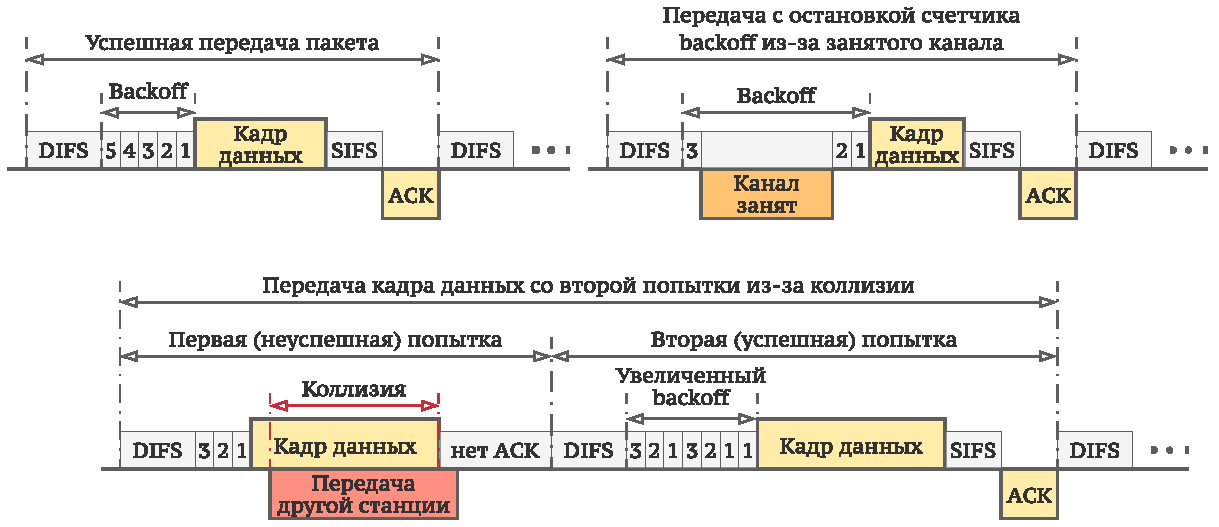
\includegraphics[width=0.9\textwidth]{chapter1/ch1_dcf}
	\caption{Организация доступа к каналу при использовании простейшей версии механизма DCF}
	\label{fig:ch1_dcf}
\end{figure}

В действительности, механизм DCF имеет ряд дополнительных возможностей, позволяющих увеличить эффективность передачи. Во-первых, если передаваемые данные имеют достаточно большой размер, перед их передачей станция может отправить кадр RTS (Request to Send), в котором передается ожидаемое время занятости канала. В ответ на RTS получатель передает CTS (Clear to Send), которым подтверждает готовность вести прием. Этот механизм позволяет решить проблему скрытых станций. Во-вторых, после успешной передачи станция может начать отсчет backoff (так называемый post-backoff) и, если новый пакет придет от сетевого уровня до того, как отсчет закончится, ему потребуется ждать передачи меньше времени. Количество попыток передачи пакета ограничено, и при его достижении пакет, вообще говоря, отбрасывается как недоставленный. Стоит также отметить, что при передаче больших пакетов может использоваться дефрагментация, и отдельные фрагменты могут передаваться без дополнительных отсчетов backoff. В диссертационной работе эти механизмы не учитываются, однако в дальнейшем их можно учесть для повышения точности моделирования. Что касается post-backoff и передачи группы кадров получившей доступ к каналу станцией (EDCF), для их адекватного учета нужно использовать более сложные методы описания времени передачи, например "--- марковские процессы обслуживания (MSP).


%%% --------------------------------------------
\subsection{Обзор исследований производительности беспроводных каналов связи}\label{sec:ch1_wifi_observe}
%%% --------------------------------------------

Из всех характеристик беспроводных каналов, в диссертационном исследовании основной интерес представляет время, необходимое для передачи одного сообщения. Для оценки длительности передачи сообщений, а также для оценки пропускной способности канала часто используются марковские или полумарковские случайные процессы. В таких моделях состояние случайного процесса описывает состояние канала (например, <<канал занят, ждать ещё два слота>> или <<ведётся передача>>), и производится оценка либо доли времени, которое процесс находится в определенных состояниях, либо времени, нужного для попадания в некоторое состояние. Использованию марковских и полумарковских процессов для анализа производительности беспроводных сетей на основе CSMA/CA посвящено большое количество работ, одной из ключевых является статья Bianchi \cite{Bianchi2000}, в которой была предложена марковская цепь, моделирующая работу станции сети IEEE 802.11 под управлением механизма доступа DCF. Состояния цепи соответствуют слотам ожидания backoff и попыткам передачи. Важным допущением модели является постоянство условной вероятности коллизии при передаче, а также насыщенный режим работы. С помощью предложенной цепи рассчитывается пропускная способность сети в насыщенном режиме. Полумарковские процессы также часто используются для описания работы беспроводной сети. Например, в работе \cite{Lauwens2010} предложен полумарковский процесс, моделирующий работу канального уровня сети IEEE 802.15.4-2006. Вместе с полумарковским процессом рассматривается процесс восстановления, моделирующий физический уровень. Предложенная авторами аналитическая модель используется для оценки пропускной способности сети, а кроме этого -- оценки интервалов между успешными передачами и распределения длительности ожидания в backoff.

Так как DCF является наиболее базовым механизмом доступа, используемым в сетях IEEE 802.11, анализ длительности передачи пакетов в каналах DCF подробно рассматривался в большом числе работ (например, \cite{Chat2002, Banchs2006, Sakurai2007, Vardakas2007, Dong2008, Hung2007, Tickoo2008, Felemban2011, Haghani2011, Dai2013, Issar2005}). Отметим, что многие из этих работ основаны на марковском процессе, описанном Bianchi \cite{Bianchi2000}. Так, Chatzimisios и соавторы в работе \cite{Chat2002} описывают простейшую модель для расчета среднего времени передачи пакетов, основанную на модели Bianchi, предполагая ограниченное количество попыток передачи. В работе \cite{Banchs2006} также представлена аналитическая модель для вычисления задержек в передаче пакетов в ad-hoc сети IEEE 802.11 под управлением DCF в нагруженном режиме; помимо самой задержки, авторы анализируют сценарии использования сети для передачи голосовых и обычных данных. Авторы \cite{Sakurai2007} рассматривают работу ad-hoc сети в насыщенном режиме под управлением механизма DCF, получают аналитические выражения для математического ожидания и дисперсии времени обслуживания пакета, учитывая при этом ограниченное количество попыток передачи. Авторы также дают выражение для производящей функции моментов времни передачи пакета и исследуют функцию распределения этого времени. В работе \cite{Vardakas2007} рассматривается задержка, учитывающая также нахождение пакета в очереди. В работе \cite{Dong2008} Dong и соавторы изучают работу ad-hoc сети в ненасыщенном режиме, предполагая экспоненциальное распределение интервалов времени между поступлениями пакетов, и, помимо анализа времени обслуживания на отдельных узлах, рассматривают задержку при передаче по многошаговым маршрутам, учитывая наличие скрытых станций. Также проблеме измерения времени передачи при наличии скрытых станций посвящена работа \cite{Hung2007}. В работе \cite{Tickoo2008} представлен не только делательный анализ времени передачи пакетов в ad-hoc сети в ненагруженном режиме, но и рассматривается случай передачи группы пакетов при использовании механизма EDCA из IEEE 802.11e. Felemban и Ekici в работе \cite{Felemban2011} анализируют время передачи пакетов в одношаговых ad-hoc сетях, уточняя модель Bianchi за счет введения дополнительных марковских цепей в backoff-состояниях; ими также рассматривается случай ненасыщенной работы сети (при этом предполагается, что пакеты поступают в пуассоновском потоке). Также ненагруженный режим рассматривается в работе \cite{Duffy2005}. Еще один детальный анализ производительности ad-hoc сетей, включая длительности передачи пакетов, представлен в работе \cite{Dai2013}. Следует также выделить работу \cite{Issar2005}, в которой время передачи пакета описано как PH-распределение.

%Отметим, что целью нашей работы является не столько моделирование времени передачи пакетов на отдельных каналах, сколько использование полученных моделей времени для использования в составе тандемных сетей массового обслуживания типа $MAP/PH/1/N \rightarrow \dots \rightarrow \bullet/PH/1/N$ для оценки характеристик беспроводных сетей с линейной топологией. Хотя далее мы предлагаем использовать простую полумарковскую модель для анализа времени передачи пакетов в сети, работающей в насыщенном режиме (и показываем, что в некоторых случаях это дает хорошую оценку), для уточнения результатов можно использовать оценки времени передачи из приведенных выше работ, в особенности это касается ненасыщенного режима работы сети.

Ряд исследований рассматривают и сравнивают различные схемы доступа, используемые в сетях IEEE 802.11. Можно выделить работу \cite{Gao2005}, в которой рассматриваются режимы доступа EDCA и HCF, определенные в стандарте IEEE 802.11е и обсуждается их применимость к передаче данных мультимедиа. Также можно выделить работу \cite{Charfi2012}, авторы которой приводят описание как основных методов доступа DCF, PCF, EDCA, HCCA, так и дополнения, вводимые расширениями IEEE 802.11ac и IEEE 802.11ad (следует отметить, что статья вышла в 2012 году, когда расширения IEEE 802.11ac и IEEE 802.11ad еще находились на стадии разработки). Анализ производительности методов доступа EDCA \cite{Engelstad2006, Hazra2011, Kong2004, Liu2007, Inan2009, Misic2012, YanfengZhu2006} и HCCA \cite{Harsha2006, Ghazizadeh2009, Rashd2006}, введенных в стандарте IEEE 802.11e, широко рассмотрен в литературе. В работе \cite{Engelstad2006} с помощью аппарата марковских цепей и систем M/G/1 анализируется пропускная способность канала связи при использовании метода EDCA, а также полная задержка пакетов, включая время ожидания в очереди. В работе \cite{Hazra2011} также предлагается использовать марковскую цепь для анализа производительности, а предложенная авторами модель учитывает блочные подтверждения и агрегацию кадров. Еще один пример марковской цепи, используемой для анализа EDCA, приведен в работе \cite{Kong2004}. Авторы работы \cite{Liu2007} анализируют задержки и пропускные способности каналов под управлением EDCA при передачи разных типов трафика. В работе \cite{Misic2012} приводится большая аналитическая модель, позволяющая анализировать производительность EDCA в ненагруженном режиме. Следует также отметить работу \cite{YanfengZhu2006}, в которой авторы предлагают для анализа DCF и EDCA использовать модель PH/PH/1. В работе \cite{Harsha2006} авторы предлагают модель для анализа производительности канала связи при передаче голоса с использованием метода доступа HCCA и данных с использованием метода доступа EDCA. В работе \cite{Ghazizadeh2009} предлагается модель массового обслуживания MAP/PH/1 с приоритетами и периодами отдыха для анализа метода доступа HCCA.  Авторы работы \cite{Rashd2006} также используют марковскую систему массового обслуживания с отдыхами для моделирования HCCA.

В более поздних работах исследуются нововведения в протоколы MAC-уровня, появившихся в дополнениях IEEE 802.11ac и IEEE 802.11ad. Так, в работе \cite{Khan2017} анализируется производительность канала IEEE 802.11ac с использованием MIMO, учитывающая особенности как канального, так и физического уровня; нужно отметить, что в качестве модели канала используется, фактически, модель Bianchi \cite{Bianchi2000}. В работе \cite{Ong2011} приводится сравнение производительности IEEE 802.11n и IEEE 802.11ac, акцент сделан на исследовании механизмов агрегации кадров. Авторы работы \cite{Chandra2017} предлагают марковскую модель для анализа производительности миллиметровых каналов IEEE 802.11ad, учитывая такие особенности канала, как разделение пространства вокруг базовой станции на сектора.


%%%%%%%%%%%%%%%%%%%%%%%%%%%%%%%%%%%%%%%%%%%%%%%%%%%%%%%%%%%%%%%%%%%%%%%%%%%%%%%%
\section{Методы исследования задержек в многошаговых беспроводных сетей}\label{sec:ch1_qs}
%%%%%%%%%%%%%%%%%%%%%%%%%%%%%%%%%%%%%%%%%%%%%%%%%%%%%%%%%%%%%%%%%%%%%%%%%%%%%%%%

Способы получения оценок задержек и пропускной способности сетей можно разбить на три группы: стендовые, имитационные и аналитические. Стендовые измерения проводятся на реальной сети или ее макете. Эти измерения наиболее точные, но очень ресурсозатратные, трудоемкие и не всегда осуществимые. Имитационные измерения проводятся с помощью разчлиных систем имитационного моделирования, в которых сеть моделируется с помощью набора алгоритмов. Обычно эти алгоритмы воспроизводят работу моделируемых протоколов с высокой точностью. Наиболее популярные открытые системы имитационного моделирования NS-3 и OMNeT++ содержат реализации большинства распространенных сетевых протоколов, в том числе IEEE 802.11 (WiFi) и IEEE 802.3 (Ethernet). Преимущество имитационного моделирования "--- высокая точность, сопоставимая с измерением на стенде, и возможность получить множество различных характеристик с одного запуска. Главный недостаток "--- высокая вычислительная сложность. Наконец, аналитические методы позволяют найти оценки исследуемых параметров с помощью математических моделей. Чаще всего эти математические модели абстрагируются от всего, что не связано непосредственно с исследуемыми характеристиками. В зависимости от конкретной модели, оценки возможно получить гораздо быстрее, чем с помощью имитационного моделирования. Однако, из-за высокой степени абстракции, ошибки могут быть достаточно высокими.

Для аналитической оценки времени, которое требуется пакету для прохождения по сети, чаще всего используется аппарат теории массового обслуживания. В рамках этого подхода интервалы между поступающими в сеть пакетами и времена передачи пакетов в каналах связи моделируются случайными распределениями, а память в интерфейсах коммутаторов "--- очередями, в которых пакеты ожидают начала обслуживания. От того, насколько удачно выбраны случайные распределения, зависит точность полученных результатов. Помимо оценки задержек, модели массового обслуживания позволяют оценить необходимую емкость очередей и оценить вероятность потери пакетов из-за их переполнений.

Выбор модели входящего потока, то есть распределений интервалов между поступлениями пакетов в сеть, зависит от передаваемого сетью трафика. В общем случае, сетевой трафик является коррелированным \cite{Heyman2003, Klemm2003}. Для представления такого трафика можно использовать модель марковских коррелированных потоков (Markovian Arrival Process, MAP).

Время передачи пакета в канале связи складывается из ожидания начала передачи, непосредственно времени передачи пакета, а также времени ожидания и получения подтверждения доставки (если протокол реализует подтверждения). Если канал ненадежен и в нем возможны потери, то приходится также учитывать неуспешные попытки передачи. Таким образом, выбор модели распределения времени обслуживания зависит от схемы доступа, которая используется в канале связи, окружения и размеров передаваемых пакетов. Для моделирования времени передачи можно использовать распределения фазового типа (Phase-Type, PH), или более общую коррелированную модель "--- марковские процессы обслуживания (Markovian Service Process, MSP). В диссертационном исследовании будем использовать PH-распределения, но многие выводы можно обощить и на случай MSP.


%%% --------------------------------------------
\subsection{Открытые сети массового обслуживания с марковскими потоками заявок и обслуживанием фазового типа}
\label{sec:ch1_qs_map_ph}
%%% --------------------------------------------

Для анализа характеристик многошаговых телекоммуникационных сетей используются модели открытых тандемных сетей массового обслуживания \cite{Vishnevskii2017, VishnevskyDudin2018}. Такие модели состоят из обслуживающих устройств с очередями (узлов), последовательно соединенных друг с другом (см. рис.~\ref{fig:ch1_qs}). Для простоты, будем считать, что весь внешний трафик поступает на первый узел, и передается последовательно через все промежуточные узлы. В более общем случае в сети может присутствовать кросс-трафик, то есть поступления пакетов снаружи на промежуточные узлы, а маршрутизация может быть сложнее, например "--- пакеты могут передаваться вперед через несколько узлов или даже назад, образуя циклы.

\begin{figure}[ht]
  \centering
   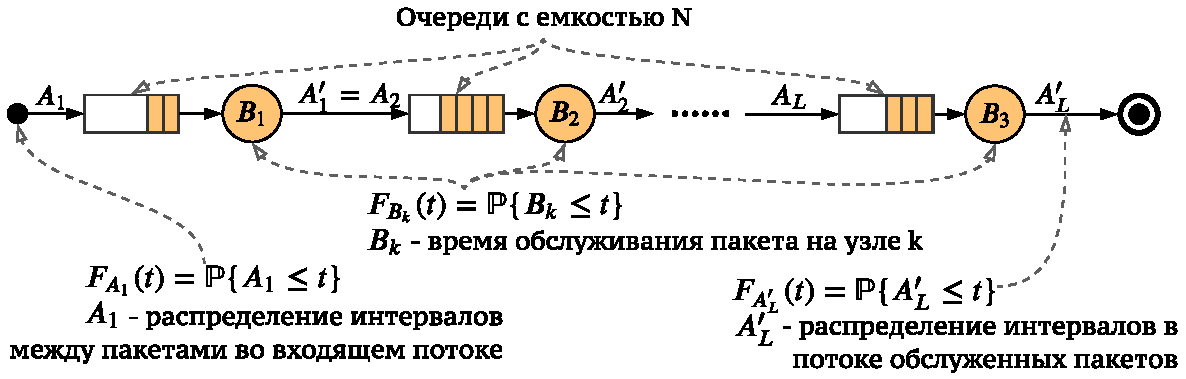
\includegraphics [scale=0.8] {chapter1/ch1_qs}
  \caption{Открытая сеть массового обслуживания с линейной топологией}
  \label{fig:ch1_qs}
\end{figure}

Если в качестве распределения времени обслуживания использовать PH-распределения, а в качестве модели входящего трафика "--- MAP-потоки, то выходящий поток обслуженных пакетов из узла MAP/PH/1/N будет также MAP \cite{Dudin2000}. Благодаря этому свойству рассчитывать характеристики открытой сети с линейной топологией с узлами MAP/PH/1/N можно с помощью простой итерационной процедуры, которая будет рассматриваться в главе 4.

PH-распределения являются обощением экспоненциальных распределений и могут использоваться для приближения любого непрерывного распределения на множестве неотрицательных чисел (см., например, \cite{Johnson1989}). Случайная величина $B$ имеет PH-распределение, если ее можно выразить как время, проведенное в некоторой непрерывной цепи Маркова с генератором $\widetilde{S}$, до попадания в поглощающее состояние. PH-распределение задается квадратной матрицей $S \in \mathbb{R}^{V \times V}$ и вектором начального распределения $\overline{\tau} \in \mathbb{R}^V$, для которых должно выполняться:

\begin{equation}\label{eq:ch1_ph_def}
        \begin{aligned}
                &\tilde{S} = \begin{bmatrix}
                        S  & -S\mathbf{1} \\
                        \mathbf{0} &  0
                \end{bmatrix} \mbox{"--- инфинитезимальная матрица,}\\
                &\forall i = \overline{1,V}: \: 0 \leq \tau_i \leq 1, \qquad
                        \sum\limits_{i=1}^{V} \tau_i = 1.
        \end{aligned}
\end{equation}
Функция распределения случайной величины $B \sim PH(S, \overline{\tau})$ имеет вид $F_B(x) = \mathbb{P}\{B < x\} = 1 - \overline{\tau} e^{Sx} \mathbf{1}$~\cite{Buchholz2014}.

Марковские входные потоки (MAP) были впервые описаны в работах Neuts \cite{Neuts1979}. В ряде последующих исследований~\cite{Heyman2003, Klemm2003, Scott2003} было показано, что использование MAP-потоков позволяет достаточно точно моделировать сетевой трафик. MAP-поток $A \sim MAP(D_{0},D_{1})$ является обобщением PH-распределений и позволяет учесть корреляцию между значениями с лагом $k$. Распределения интервалов между событиями в MAP-потоке описываются PH-распределениями с одинаковыми матрицами $S \equiv D_0$, но меняющимися начальными векторами $\overline{\tau}_i$, зависящими от того, в каком состоянии находился процесс при появлении предыдущего события. MAP-поток определяется с помощью двух матриц, сумма которых $D=D_{0}+D_{1} \in \mathbb{R}^{W \times W}$ "--- инфинитезимальный генератор марковской цепи с непрерывным временем, управляющей переходами между состояниями процесса. Матрицы удовлетворяют ограничениям:

\begin{equation}\label{eq:ch1_map_def}
    \begin{aligned}
        &\forall i: \sum\limits_{j=1} \{D\}_{ij} = 0, \quad
        \forall i \neq j: \{D\}_{ij} \geq 0, \quad
        \forall i: \{D\}_{ii} \leq 0\\
        &\forall i, j: \{D_{1}\}_{ij} \geq 0,\quad
        \forall i \neq j: \{D_{0}\}_{ij} \geq 0, \quad
        \forall i: \{D_{0}\}_{ii} \leq 0.
    \end{aligned}
\end{equation}

Более подробно свойства MAP-потоков и PH-распределений, которые потребуются для расчета характеристик тандемных сетей массового обслуживания, будут описаны в главе 4.

Помимо MAP-потока, иногда рассматриваются его обобщения на случай группового поступления пакетов (Batch MAP, BMAP)~\cite{Lucantoni1993, Dudin2000, VishnevskyDudin2018} или поступлений пакетов с разными приоритетами (Marked Markovian Arrival Process, MMAP)~\cite{HE2001, VanHoudt2012, Buchholz2010, Klimenok2020}. В обоих случаях вместо двух матриц $D_0$ и $D_1$ рассматривается набор матриц $D_i, i = \overline{0,K}$, где матрицы $D_i$ при $i > 0$ соответствуют поступлению группы $i$ пакетов (для BMAP) или пакета $i$-го типа (для MMAP).

Одна из основных проблем, возникающих при получении численных характеристик сетей массового обслуживания с узлами MAP/PH/1/N "--- экспоненциальный рост пространства состояний, из-за которого точный расчет возможен только для задач небольшой размерности. В связи с этим, для практического использования этой модели важно найти эффективные методы расчета характеристик тандемной сети массового обслуживания.

Исследованиям сетей массового обслуживания с MAP-потоками и PH-распределениями времени обслуживания посвящено множество работ. Например, в~\cite{Strelen1998, Henderson1990, Strelen1997, Strelen1997a} предлагаются методы вычисления характеристик сетей массового обслуживания на основе методов декомпозиции и представления искомых характеристик в форме произведений. В ряде работ акцент сделан на тандемных сетях массового обслуживания и изучениии их характеристик \cite{Kim2018, Kim2012, Kim2007, Buchholz2006}, а также исследованию выходных потоков из систем массового обслуживания с марковскими входными потоками \cite{Bean1998, Lian2011}.

%%% --------------------------------------------
\subsection{Методы восстановления PH-распределений и MAP-потоков}\label{sec:ch1_qs_ph_fitting}
%%% --------------------------------------------

Методы поиска PH-распределений и MAP-потоков в диссертационном исследовании будут применяться для решения двух задач: для поиска распределений, моделирующих время передачи пакетов в каналах связи, и для поиска MAP-потоков меньшей размерности, аппроксимирующих потоки обслуженных пакетов на выходе из очередного узла тандемной сети.

Для поиска PH-распределения или MAP-потока можно использовать два подхода: принцип максимального правдоподобия и метод моментов. В первом случае необходима выборка значений распределения, на которой максимизируется функция правдоподобия. Существует ряд реализаций, основанных на методе максимизации ожидания (EM-процедуре) для MAP-потоков \cite{Horvath2013,Ephraim2009,Buchholz2003,Okamura2009} и PH-распределений \cite{Asmussen1996,Bobbio1992,Thummler2005,Okamura2013,Okamura2011,ElAbdouniKhayari2003}. Главное ограничение метода "--- высокая вычислительная сложность, что ограничивает его использование в итерационных алгоритмах, где его необходимо применять многократно. Из-за этого в диссертационном исследовании этот подход не будет использоваться, хотя он оказывается достаточно удобным при поиске MAP-потоков и PH-распределений при моделировании реальных входящих данных, полученных, например, из сетевого дампа.

Второй подход основан на методе моментов. Он применяется как для PH-распределений \cite{Osogami2006,Bobbio2005,Johnson1989,Telek2003,Horvath2013,VandenBosch2000,Horvath2007,Schmickler1992}, так и для MAP-потоков \cite{TelekHorvath2007,Bodrog2010,Bodrog2008,Horvath2005,Schmickler1992,Casale2010}. В первом случае PH-распределение строится по известным значениям первых моментов $m_1, m_2, \dots m_K$ случайной величины, во втором также могут учитываться значения коэффициентов автокорреляции $l$-го порядка (с лагом $l$) $\rho_1, \rho_2, \dots, \rho_L$.

Сложность применения метода моментов заключается в том, что точные области существования PH-распределений и MAP-потоков заданной размерности $W$, то есть множество значений моментов $m_1, m_2, \dots m_K$ и коэффициентов автокорреляции $\rho_1, \rho_2, \dots, \rho_L$ при сколь угодно больших $K$ и $L$, для которых существует PH-распределение или MAP-поток размерности $W$, имеют сложный вид~\cite{Bobbio2005,Osogami2006,TelekHorvath2007,Bodrog2008,Bodrog2010}. Другими словами, при известных значениях моментов и коэффициентов автокорреляции сложно не только найти PH-распределение или MAP-поток минимально возможного порядка, но и даже определить этот порядок. При этом, хорошо известны грубые оценки, связывающие размерность и значения моментов. Например, в работе \cite{Aldous1987} доказано, что среди всех PH-распределений заданного размера наименьшее значение коэффициента вариации достигается на распределении Эрланга, что позволяет грубо оценить снизу размерность искомого PH-распределения при известных первом и втором моменте. Есть методы, позволяющие находить распределения малого порядка, но не для любых наборов значений моментов. Например, в работе \cite{Telek2003} исследуется область существования ациклических PH-распределений второго порядка APH(2), а в работе \cite{Bodrog2010} Bodrog и соавторы исследуют область существования MAP-потоков второго порядка. Telek и Horvath \cite{TelekHorvath2007} описывают минимальные формы PH-распределений и MAP-потоков (марковская, жорданова и прочие формы), а также преобразования между ними. Авторы предлагают алгоритм оптимизации матриц $D_0$ и $D_1$, позволяющий минимизировать целевую функцию, зависящую от $B^{-1}D_{0}B$ и $B^{-1}D_{1}B$ посредством поиска матрицы преобразования $B$. Предложенный метод позволяет улучшить MAP-поток, который был получен любым другим методом.

Если ограничения на порядок существенны, то в общем случае приходится искать такой MAP-поток $X \sim MAP(D_0, D_1)$ (PH-распределение $Y \sim PH(S, \overline{\tau})$), чтобы выполнялись ограничения \eqref{eq:ch1_map_def} (для PH-распределения "--- \eqref{eq:ch1_ph_def}), и достигался минимум функции ошибки при заданных весах $\overline{w}$:

$$
\begin{aligned}
\mathcal{L}_{\text{MAP}}(X; \overline{m}, \overline{\rho}, \overline{w}) &=
\sum\limits_{k=1}^K w_k (m'_k - m_k)^2 + \sum\limits_{l=1}^L w_{K+l} (\rho'_l - \rho_l)^2 \rightarrow \min\\
\mathcal{L}_{\text{PH}}(Y; \overline{m}, \overline{w}) &=
\sum\limits_{k=1}^K w_k (m'_k - m_k)^2 \rightarrow \min
\end{aligned}
$$
Здесь $m'_k$ "--- $k$-й момент MAP-потока $X$ или PH-распределения $Y$, а $\rho'_l$ "--- коэффициент автокорреляции $X$ с лагом $l$.

При поиске PH-распределений чаще всего накладываются ограничения на структуру матрицы $S$, то есть поиск ведется по некоторому подсемейству распределений. Есть реализации метода моментов \cite{Johnson1989, Bobbio2005, Horvath2007, Horvath2013}, которые позволяют находить распределения по произвольному набору моментов. В работе Johnson и Taafe \cite{Johnson1989} предлагают искать PH-распределения по заданным трем моментам в виде гиперэрланговского распределения с двумя цепочками Эрланга одинакового порядка. Bobbio и соавторы \cite{Bobbio2005} предлагают метод поиска ациклических PH-распределений APH(n) минимального порядка $n$ также по первым трем моментам; кроме того, авторы описывают границы значений первых трех моментов для распределений APH(n) при известном $n$. В работе \cite{Horvath2013} Horvath и соавторы предлагают метод поиска по произвольному числу первых моментов специального подкласса PH-распределений "--- обобщенных гиперэрланговских распределений. Метод позволяет находить множество допустимых PH-распределений, из которых можно выбрать наиболее подходящее по той или иной метрике. Casale и соавторы \cite{Casale2010} предлагают метод поиска MAP-потоков по первым трём моментам и коэффициентам автокорреляции как композиции MAP-потоков меньших размеров (метод композиции через кронекерово произведение, Kronecker Product Composition, KPC).

Если задача состоит в поиске MAP-потока $X'$ с теми же характеристиками, что и MAP-поток $X$, но имеющего меньший порядок, то можно использовать и другие подходы. Например, простой метод сокращений пространства состояний основан на идее о том, что некоторые состояния MAP-потока большой размерности избыточны, и их можно удалить. Этот метод применим для систем $MAP/PH/1$ и $MAP/PH/1/N$, в которых коэффициент загрузки достаточно мал. Например, авторы работы \cite{Horvath2010} рассматривают выходной поток (обслуженных пакетов) системы $MAP/MAP/1$ и предлагают удалять блоки матриц $D_0,\,D_1$, соответствующие числу пакетов в системе свыше заданного уровня $N$.

В диссертационной работе для поиска PH-распределений и MAP-потоков будет использоваться метод моментов, а именно "--- простой метод поиска PH-распределений по первым трем моментам в виде распределений гиперэрланга с двумя цепями одинаковых порядков, предложенный в работе Johnson и Taafe \cite{Johnson1989}. При поиске MAP-потока этот метод будет использоваться для расчета матрицы $D_0$, а поиск матрицы $D_1$ будет производиться отдельно по заданным коэффициентам автокорреляции, как предложено в работе Horvath и соавторов \cite{Horvath2005}. Как показали численные эксперименты, эта комбинация методов просто реализуется, работает достаточно хорошо и стабильно и позволяет находить распределения за короткое время, хотя порядки могут быть несколько больше, чем в альтернативных методах. Время работы особенно критично, так как в численном эксперименте требовалось рассчитать характеристики нескольких сотен сетей с узлами $MAP/PH/1/N$.



%%%%%%%%%%%%%%%%%%%%%%%%%%%%%%%%%%%%%%%%%%%%%%%%%%%%%%%%%%%%%%%%%%%%%%%%%%%%%%%%
\section{Методы построения распределённых систем радиочастотной идентификации}
%%%%%%%%%%%%%%%%%%%%%%%%%%%%%%%%%%%%%%%%%%%%%%%%%%%%%%%%%%%%%%%%%%%%%%%%%%%%%%%%

С момента появления технологии RFID ведутся исследования в области создания систем управления считывателями и промежуточного программного обеспечения (Middleware). Хороший обзор ранних подходов и практически реализованных систем приведен в работе Al-Jaroodi и соавторов \cite{Al-Jaroodi2009}, где они рассматривают общие требования к промежуточному программному обеспечению для RFID и анализируют семь различных систем с точки зрения надёжности, масштабируемости, балансировке нагрузки, возможности управления данными и безопасности. В более позднем обзоре Razzaque и соавторы \cite{Razzaque2016}, рассматривая RFID уже в качестве неотъемлемой части Интернета вещей (Internet of Things, IoT), расширяют список требований, предъявляемых к промежуточному программному обеспечению, рассматривая требования к программным интерфейсам, необходимость реализации программного обеспечения в рамках сервисно-ориентированной модели Software-as-a-Service (SaaS) и Everything-as-a-Service (XaaS).

Для подключения RFID-считывателей к системам управления используются стандартные протоколы, которые поддерживаются большинством производителей. Протокол Low Level Reader Protocol (LLRP) \cite{StdLlrp} определяет низкоуровневый интерфейс между считывателем и контроллером. Этот протокол позволяет выполнять произвольные операции доступа и инвентаризации, настраивать параметры радиоинтерфейса считывателя, получать данные о состоянии радиоканала и диагностические данные о работе считывателя. Протокол LLRP поддерживается большинством существующих считывателей. Стандарт определяет возможность работы протокола по каналам TLS. Помимо LLRP, организация EPCglobal опубликовала несколько стандартов \cite{StdRm, StdDci, StdAle1, StdAle2}, которые можно использовать при разработке считывателя и системы управления. Стандарт <<Reader Management 1.0.1 (RM)>> \cite{StdRm} определяет модель системы и MIB (Management Information Base) для сбора данных о состоянии работы считывателя через протокол SNMP. Стандарт <<Discovery, Configuration, and Initialization (DCI) for Reader Operations>> \cite{StdDci} позволяет считывателю, контроллерам и LLRP-клиентам находить друг друга в сети, производить аутентификацию между контроллерами и считывателями, управлять работой считывателей, загружать новые образы программного обеспечения и выполнять прочие служебные функции. Стандарт <<Application Level Events (ALE) Standard>> \cite{StdAle1, StdAle2} описывает рекомендации по разработке промежуточного программного обеспечения. Кроме стандартов EPCglobal, существует спецификация интерфейса между считывателем и контроллером от альянса RAIN RFID \cite{StdRainRci}. Эта спецификация более высокоуровневая, по сравнению с LLRP. Она описывает основные действия, включая конфигурацию и получение статуса считывателя, настройки радиопротокола, доступ к меткам. Спецификация определяет сообщения, передаваемые между считывателем и конроллером, в формате JSON.

В целом ряде ранних исследовательских работ \cite{Hoag2006,Yu2009,XiuLi2012,Koutsoubelias2007,Abad2012,Chien-ChangHsu2008,Floerkemeier2007} рассматриваются детали архитектуры и подходов к построению промежуточного программного обеспечения, причем материал некотрых из них и на сегодняшний день представляет интерес. Например, Hoag и Thompson в работе \cite{Hoag2006} выделяют два уровня архитектуры: уровень агентов и уровень RFID-приложений. Предложенная архитектура допускает подключение различного оборудования (считыватели, принтеры меток, базы данных и пр.) через специальных модулей--агентов, использующих для обмена сообщениями унифицированный транспортный уровень, на котором реализуются как односторонние обмены сообщениями, так и многоадресные соединения для связи типа <<публикация--подписка>>. Архитектура системы на основе механизма подписок также рассматривается в работе Yu и Lai~\cite{Yu2009}. В работе~\cite{XiuLi2012} описывается двухуровневая архитектура промежуточного программного обеспечения RFID с фильтрацией и агрегацией данных, а в работе~\cite{Koutsoubelias2007} предлагается построение промежуточного программного обеспечения с использованим адаптеров, предоставляющих унифицированный интерфейс для подключения считывателей. Авторы \cite{Chien-ChangHsu2008} предлагают модель системы управления считывателями и промежуточным программным обеспеченим, направленную на повышение отказоустойчивости. Наконец, ещё один ранний проект открытого промежуточного программного обеспечения для RFID (Accada) был предложен в работе Floerkemeier и соавторов \cite{Floerkemeier2007}. В нем авторы поднимают ряд проблем, от различия между требованиями пользователей вплоть до многолучевого распространения сигналов, и предлагают оригинальные решения, например "--- использование виртуальной памяти для отложенной записи данных на метки или механизм прогнозирования длительности нахождения меток в области чтения.

В более поздних исследованиях разработчики систем управления и промежуточного программного обеспечения рассматривают RFID в более широком контексте интернета вещей (IoT). В работе \cite{Santos2019} предложена пятиуровневая модель, в которой данные со считывателя поступают в облако и обрабатываются при помощи различных микросервисов. Aazam и Huh в работе \cite{Aazam2016} рассматривают системы управления и взаимодействия с устройствами (в частности, с RFID-считывателями и метками) в контексте интернета вещей (IoT), интернета всего (Internet of Everything, IoE) и туманных вычислений (Fog Computing). Например, в работе \cite{Schreiber2012} Schreiber с соавторами предлагают архитектуру промежуточного программного обеспечения, позволяющего единообразно работать с RFID-считывателями и сенсорами. Помимо детального описания архитектуры, авторы также предлагают SQL-подобный язык, позволяющий пользователю строить запросы к системе, не вдаваясь в специфику того ли иного устройства. В более ранней работе \cite{Cho2007} Cho и соавторы рассматривают распределенную систему, позволяющую не просто идентифицировать объекты, но связывать данные о них с показателями сенсоров.

Хотя в большинстве работ промежуточное программное обеспечение включает в себя функции как для получения и обработки данных о прочитанных метках, так и функции управления и мониторинга состояния считывтелей, некоторые авторы допускают их разнесение. Например, Kamoun в работе \cite{Kamoun2009} предполагает, что системы управления считывателями лучше не рассматривать в контексте промежуточного программного обеспечения, оставив последнему функции по работе с данными. В работе \cite{JongyoungLee2006} производится анализ и выбор метрик производительности промежуточного программного обеспечения для RFID. Авторы рассматривают в качестве метрик зависимости загрузки системы (использование процессоров и памяти) и времени отклика на запросы клиентов от числа подключенных считывателей, числа подключенных приложений (клиентов), а также количества читаемых каждым считывателем меток. Также авторы описывают дизайн системы анализа производительности промежуточного программного обеспечения для RFID и приводят краткое описание собственной реализации.

Многие исследования направлены на разработку программного обеспечения для специализированных применений RFID. Например, в работе \cite{Henao2019} описывается архитектура информационной системы, в которой один терминал (клиент) подключается ко множеству считывателей (серверов), для применения на автомобильном заводе. Статья \cite{Figueroa2019} посвящена описанию системы отслеживания местонахождения людей с помощью имплантированных RFID-чипов под кожу. В работе \cite{Zhang2018} описана информационная система для управления библиотечным фондом с использованием RFID, авторы \cite{Li2010} описывают архитектуру и опыт реализации RFID-системы на фабрике по выпуску одежды, а в работе \cite{Shah2016} предлагается использовать RFID для систем обеспечения безопасности перевозки школьников в автобусах. В статье \cite{Chamekh2017} рассматривается использование RFID в области фармацевтики для контроля за качеством лекарств и отслеживанием контрафакта. Работы \cite{Rouchdi2018,Baskoro2018} посвящены системам отслеживания багажа в аэропортах с помощью RFID.

Помимо технической стороны разработки информационных систем с использованием RFID, есть ряд вопросов этики и безопасности, поскольку данные на метках находятся в тесной связи с людьми и бизнесом. Хорошую подборку и анализ как преимуществ внедрения RFID, так и проблем, связанных с этим (в частности, кражей данных и отношением людей к сбору данных о себе), можно найти в ранней работе \cite{Thompson2007}. В работе \cite{Figueroa2019} предлагается использовать блокчейн для распределенного контроля доступа к меткам. Бельский и соавторы \cite{Belsky2021} исследуют безопасность систем RFID и приводят описание моделей угроз. Авторы работы \cite{Bashir2011} описывают требования к распределенной системе управления мобильными RFID-считывателями, уделяя особое внимание вопросам безопасности. Также стоит выделить работу Fouladgar и Afifi \cite{Fouladgar2007}, в которой они предлагают безопасный протокол делегирования из доверенной центральной информационной системы прав на идентификацию меток считывателям.





\section{Заключение}\label{sec:ch1_conclusion}

В главе была описана общая структура системы радиочастотной идентификации транспорта, разработке и исследованию которой посвящена диссертационная работа. Выделены ключевые компоненты системы: RFID считыватели, метки, телекоммуникационная сеть и центр обработки данных; для каждого из компонентов поставлены задачи, решаемые в диссертационном исследовании.

После постановки задач исследования, в главе были описаны технологии, используемые в распределенной системе радиочастотной идентификации, и математические методы, используемые для их исследования. По всем упомянутым технологиям и методам был приведен обзор литературы и актуальных научных исследований. Также в общих чертах были выделены отличия и новизна предложенных в диссертации методов и подходов от существующих в литературе.






%\section{Форматирование текста}\label{sec:ch1/sec1}
%
%Мы можем сделать \textbf{жирный текст} и \textit{курсив}.
%
%\section{Ссылки}\label{sec:ch1/sec2}
%
%Сошлёмся на библиографию.
%Одна ссылка: \cite[с.~54]{Sokolov}\cite[с.~36]{Gaidaenko}.
%Две ссылки: \cite{Sokolov,Gaidaenko}.
%Ссылка на собственные работы: \cite{vakbib1, confbib2}.
%Много ссылок: %\cite[с.~54]{Lermontov,Management,Borozda} % такой «фокус»
%%вызывает biblatex warning относительно опции sortcites, потому что неясно, к
%%какому источнику относится уточнение о страницах, а bibtex об этой проблеме
%%даже не предупреждает
%\cite{Lermontov, Management, Borozda, Marketing, Constitution, FamilyCode,
%Gost.7.0.53, Razumovski, Lagkueva, Pokrovski, Methodology, Berestova,
%Kriger}%
%\ifnumequal{\value{bibliosel}}{0}{% Примеры для bibtex8
%    \cite{Sirotko, Lukina, Encyclopedia, Nasirova}%
%}{% Примеры для biblatex через движок biber
%    \cite{Sirotko2, Lukina2, Encyclopedia2, Nasirova2}%
%}%
%.
%И~ещё немного ссылок:~\cite{Article,Book,Booklet,Conference,Inbook,Incollection,Manual,Mastersthesis,
%Misc,Phdthesis,Proceedings,Techreport,Unpublished}
%% Следует обратить внимание, что пробел после запятой внутри \cite{}
%% обрабатывается ожидаемо, а пробел перед запятой, может вызывать проблемы при
%% обработке ссылок.
%\cite{medvedev2006jelektronnye, CEAT:CEAT581, doi:10.1080/01932691.2010.513279,
%Gosele1999161,Li2007StressAnalysis, Shoji199895, test:eisner-sample,
%test:eisner-sample-shorted, AB_patent_Pomerantz_1968, iofis_patent1960}
%\ifnumequal{\value{bibliosel}}{0}{% Примеры для biblatex через движок biber
%    \cite{patent2h, patent3h, patent2}%
%}%
%.
%
%\ifnumequal{\value{bibliosel}}{0}{% Примеры для bibtex8
%Попытка реализовать несколько ссылок на конкретные страницы
%для \texttt{bibtex} реализации библиографии:
%[\citenum{Sokolov}, с.~54; \citenum{Gaidaenko}, с.~36].
%}{% Примеры для biblatex через движок biber
%Несколько источников (мультицитата):
%% Тут специально написано по-разному тире, для демонстрации, что
%% применение специальных тире в настоящий момент в biblatex приводит к непоказу
%% "с.".
%\cites[vii--x, 5, 7]{Sokolov}[v"--~x, 25, 526]{Gaidaenko}[vii--x, 5, 7]{Techreport},
%работает только в \texttt{biblatex} реализации библиографии.
%}%
%
%Ссылки на собственные работы:~\cite{vakbib1, confbib1}
%
%Сошлёмся на приложения: Приложение~\cref{app:A}, Приложение~\cref{app:B2}.
%
%Сошлёмся на формулу: формула~\cref{eq:equation1}.
%
%Сошлёмся на изображение: рисунок~\cref{fig:knuth}.
%
%Стандартной практикой является добавление к ссылкам префикса, характеризующего тип элемента.
%Это не является строгим требованием, но~позволяет лучше ориентироваться в документах большого размера.
%Например, для ссылок на~рисунки используется префикс \textit{fig},
%для ссылки на~таблицу "--- \textit{tab}.
%
%В таблице \cref{tab:tab_pref} приложения~\cref{app:B4} приведён список рекомендуемых
%к использованию стандартных префиксов.
%
%\section{Формулы}\label{sec:ch1/sec3}
%
%Благодаря пакету \textit{icomma}, \LaTeX~одинаково хорошо воспринимает
%в~качестве десятичного разделителя и запятую (\(3,1415\)), и точку (\(3.1415\)).
%
%\subsection{Ненумерованные одиночные формулы}\label{subsec:ch1/sec3/sub1}
%
%Вот так может выглядеть формула, которую необходимо вставить в~строку
%по~тексту: \(x \approx \sin x\) при \(x \to 0\).
%
%А вот так выглядит ненумерованная отдельностоящая формула c подстрочными
%и надстрочными индексами:
%\[
%(x_1+x_2)^2 = x_1^2 + 2 x_1 x_2 + x_2^2
%\]
%
%Формула с неопределенным интегралом:
%\[
%\int f(\alpha+x)=\sum\beta
%\]
%
%При использовании дробей формулы могут получаться очень высокие:
%\[
%  \frac{1}{\sqrt{2}+
%  \displaystyle\frac{1}{\sqrt{2}+
%  \displaystyle\frac{1}{\sqrt{2}+\cdots}}}
%\]
%
%В формулах можно использовать греческие буквы:
%%Все \original... команды заранее, ради этого примера, определены в Dissertation\userstyles.tex
%\[
%\alpha\beta\gamma\delta\originalepsilon\epsilon\zeta\eta\theta%
%\vartheta\iota\kappa\varkappa\lambda\mu\nu\xi\pi\varpi\rho\varrho%
%\sigma\varsigma\tau\upsilon\originalphi\phi\chi\psi\omega\Gamma\Delta%
%\Theta\Lambda\Xi\Pi\Sigma\Upsilon\Phi\Psi\Omega
%\]
%\[%https://texfaq.org/FAQ-boldgreek
%\boldsymbol{\alpha\beta\gamma\delta\originalepsilon\epsilon\zeta\eta%
%\theta\vartheta\iota\kappa\varkappa\lambda\mu\nu\xi\pi\varpi\rho%
%\varrho\sigma\varsigma\tau\upsilon\originalphi\phi\chi\psi\omega\Gamma%
%\Delta\Theta\Lambda\Xi\Pi\Sigma\Upsilon\Phi\Psi\Omega}
%\]
%
%Для добавления формул можно использовать пары \verb+$+\dots\verb+$+ и \verb+$$+\dots\verb+$$+,
%но~они считаются устаревшими.
%Лучше использовать их функциональные аналоги \verb+\(+\dots\verb+\)+ и \verb+\[+\dots\verb+\]+.
%
%\subsection{Ненумерованные многострочные формулы}\label{subsec:ch1/sec3/sub2}
%
%Вот так можно написать две формулы, не нумеруя их, чтобы знаки <<равно>> были
%строго друг под другом:
%\begin{align}
%  f_W & =  \min \left( 1, \max \left( 0, \frac{W_{soil} / W_{max}}{W_{crit}} \right)  \right), \nonumber \\
%  f_T & =  \min \left( 1, \max \left( 0, \frac{T_s / T_{melt}}{T_{crit}} \right)  \right), \nonumber
%\end{align}
%
%Выровнять систему ещё и по переменной \( x \) можно, используя окружение
%\verb|alignedat| из пакета \verb|amsmath|. Вот так:
%\[
%    |x| = \left\{
%    \begin{alignedat}{2}
%        &&x, \quad &\text{eсли } x\geqslant 0 \\
%        &-&x, \quad & \text{eсли } x<0
%    \end{alignedat}
%    \right.
%\]
%Здесь первый амперсанд (в исходном \LaTeX\ описании формулы) означает
%выравнивание по~левому краю, второй "--- по~\( x \), а~третий "--- по~слову
%<<если>>. Команда \verb|\quad| делает большой горизонтальный пробел.
%
%Ещё вариант:
%\[
%    |x|=
%    \begin{cases}
%    \phantom{-}x, \text{если } x \geqslant 0 \\
%    -x, \text{если } x<0
%    \end{cases}
%\]
%
%Кроме того, для  нумерованных формул \verb|alignedat| делает вертикальное
%выравнивание номера формулы по центру формулы. Например, выравнивание
%компонент вектора:
%\begin{equation}
%\label{eq:2p3}
%\begin{alignedat}{2}
%{\mathbf{N}}_{o1n}^{(j)} = \,{\sin} \phi\,n\!\left(n+1\right)
%         {\sin}\theta\,
%         \pi_n\!\left({\cos} \theta\right)
%         \frac{
%               z_n^{(j)}\!\left( \rho \right)
%              }{\rho}\,
%           &{\boldsymbol{\hat{\mathrm e}}}_{r}\,+   \\
%+\,
%{\sin} \phi\,
%         \tau_n\!\left({\cos} \theta\right)
%         \frac{
%            \left[\rho z_n^{(j)}\!\left( \rho \right)\right]^{\prime}
%              }{\rho}\,
%            &{\boldsymbol{\hat{\mathrm e}}}_{\theta}\,+   \\
%+\,
%{\cos} \phi\,
%         \pi_n\!\left({\cos} \theta\right)
%         \frac{
%            \left[\rho z_n^{(j)}\!\left( \rho \right)\right]^{\prime}
%              }{\rho}\,
%            &{\boldsymbol{\hat{\mathrm e}}}_{\phi}\:.
%\end{alignedat}
%\end{equation}
%
%Ещё об отступах. Иногда для лучшей <<читаемости>> формул полезно
%немного исправить стандартные интервалы \LaTeX\ с учётом логической
%структуры самой формулы. Например в формуле~\cref{eq:2p3} добавлен
%небольшой отступ \verb+\,+ между основными сомножителями, ниже
%результат применения всех вариантов отступа:
%\begin{align*}
%\backslash! &\quad f(x) = x^2\! +3x\! +2 \\
%  \mbox{по-умолчанию} &\quad f(x) = x^2+3x+2 \\
%\backslash, &\quad f(x) = x^2\, +3x\, +2 \\
%\backslash{:} &\quad f(x) = x^2\: +3x\: +2 \\
%\backslash; &\quad f(x) = x^2\; +3x\; +2 \\
%\backslash \mbox{space} &\quad f(x) = x^2\ +3x\ +2 \\
%\backslash \mbox{quad} &\quad f(x) = x^2\quad +3x\quad +2 \\
%\backslash \mbox{qquad} &\quad f(x) = x^2\qquad +3x\qquad +2
%\end{align*}
%
%Можно использовать разные математические алфавиты:
%\begin{align}
%\mathcal{ABCDEFGHIJKLMNOPQRSTUVWXYZ} \nonumber \\
%\mathfrak{ABCDEFGHIJKLMNOPQRSTUVWXYZ} \nonumber \\
%\mathbb{ABCDEFGHIJKLMNOPQRSTUVWXYZ} \nonumber
%\end{align}
%
%Посмотрим на систему уравнений на примере аттрактора Лоренца:
%
%\[
%\left\{
%  \begin{array}{rl}
%    \dot x = & \sigma (y-x) \\
%    \dot y = & x (r - z) - y \\
%    \dot z = & xy - bz
%  \end{array}
%\right.
%\]
%
%А для вёрстки матриц удобно использовать многоточия:
%\[
%\left(
%  \begin{array}{ccc}
%    a_{11} & \ldots & a_{1n} \\
%    \vdots & \ddots & \vdots \\
%    a_{n1} & \ldots & a_{nn} \\
%  \end{array}
%\right)
%\]
%
%\subsection{Нумерованные формулы}\label{subsec:ch1/sec3/sub3}
%
%А вот так пишется нумерованная формула:
%\begin{equation}
%  \label{eq:equation1}
%  e = \lim_{n \to \infty} \left( 1+\frac{1}{n} \right) ^n
%\end{equation}
%
%Нумерованных формул может быть несколько:
%\begin{equation}
%  \label{eq:equation2}
%  \lim_{n \to \infty} \sum_{k=1}^n \frac{1}{k^2} = \frac{\pi^2}{6}
%\end{equation}
%
%Впоследствии на формулы~\cref{eq:equation1, eq:equation2} можно ссылаться.
%
%Сделать так, чтобы номер формулы стоял напротив средней строки, можно,
%используя окружение \verb|multlined| (пакет \verb|mathtools|) вместо
%\verb|multline| внутри окружения \verb|equation|. Вот так:
%\begin{equation} % \tag{S} % tag - вписывает свой текст
%  \label{eq:equation3}
%    \begin{multlined}
%        1+ 2+3+4+5+6+7+\dots + \\
%        + 50+51+52+53+54+55+56+57 + \dots + \\
%        + 96+97+98+99+100=5050
%    \end{multlined}
%\end{equation}
%
%Уравнения~\cref{eq:subeq_1,eq:subeq_2} демонстрируют возможности
%окружения \verb|\subequations|.
%\begin{subequations}
%    \label{eq:subeq_1}
%    \begin{gather}
%        y = x^2 + 1 \label{eq:subeq_1-1} \\
%        y = 2 x^2 - x + 1 \label{eq:subeq_1-2}
%    \end{gather}
%\end{subequations}
%Ссылки на отдельные уравнения~\cref{eq:subeq_1-1,eq:subeq_1-2,eq:subeq_2-1}.
%\begin{subequations}
%    \label{eq:subeq_2}
%    \begin{align}
%        y &= x^3 + x^2 + x + 1 \label{eq:subeq_2-1} \\
%        y &= x^2
%    \end{align}
%\end{subequations}
%
%\subsection{Форматирование чисел и размерностей величин}\label{sec:units}
%
%Числа форматируются при помощи команды \verb|\num|:
%\num{5,3};
%\num{2,3e8};
%\num{12345,67890};
%\num{2,6 d4};
%\num{1+-2i};
%\num{.3e45};
%\num[exponent-base=2]{5 e64};
%\num[exponent-base=2,exponent-to-prefix]{5 e64};
%\num{1.654 x 2.34 x 3.430}
%\num{1 2 x 3 / 4}.
%Для написания последовательности чисел можно использовать команды \verb|\numlist| и \verb|\numrange|:
%\numlist{10;30;50;70}; \numrange{10}{30}.
%Значения углов можно форматировать при помощи команды \verb|\ang|:
%\ang{2.67};
%\ang{30,3};
%\ang{-1;;};
%\ang{;-2;};
%\ang{;;-3};
%\ang{300;10;1}.
%
%Обратите внимание, что ГОСТ запрещает использование знака <<->> для обозначения отрицательных чисел
%за исключением формул, таблиц и~рисунков.
%Вместо него следует использовать слово <<минус>>.
%
%Размерности можно записывать при помощи команд \verb|\si| и \verb|\SI|:
%\si{\farad\squared\lumen\candela};
%\si{\joule\per\mole\per\kelvin};
%\si[per-mode = symbol-or-fraction]{\joule\per\mole\per\kelvin};
%\si{\metre\per\second\squared};
%\SI{0.10(5)}{\neper};
%\SI{1.2-3i e5}{\joule\per\mole\per\kelvin};
%\SIlist{1;2;3;4}{\tesla};
%\SIrange{50}{100}{\volt}.
%Список единиц измерений приведён в таблицах~\cref{tab:unit:base,
%tab:unit:derived,tab:unit:accepted,tab:unit:physical,tab:unit:other}.
%Приставки единиц приведены в~таблице~\cref{tab:unit:prefix}.
%
%С дополнительными опциями форматирования можно ознакомиться в~описании пакета \texttt{siunitx};
%изменить или добавить единицы измерений можно в~файле \texttt{siunitx.cfg}.
%
%\begin{table}
%    \centering
%    \captionsetup{justification=centering} % выравнивание подписи по-центру
%    \caption{Основные величины СИ}\label{tab:unit:base}
%    \begin{tabular}{llc}
%        \toprule
%        Название  & Команда                & Символ         \\
%        \midrule
%        Ампер     & \verb|\ampere| & \si{\ampere}   \\
%        Кандела   & \verb|\candela| & \si{\candela}  \\
%        Кельвин   & \verb|\kelvin| & \si{\kelvin}   \\
%        Килограмм & \verb|\kilogram| & \si{\kilogram} \\
%        Метр      & \verb|\metre| & \si{\metre}    \\
%        Моль      & \verb|\mole| & \si{\mole}     \\
%        Секунда   & \verb|\second| & \si{\second}   \\
%        \bottomrule
%    \end{tabular}
%\end{table}
%
%\begin{table}
%  \small
%  \centering
%  \begin{threeparttable}% выравнивание подписи по границам таблицы
%    \caption{Производные единицы СИ}\label{tab:unit:derived}
%    \begin{tabular}{llc|llc}
%        \toprule
%        Название       & Команда                 & Символ              & Название & Команда & Символ \\
%        \midrule
%        Беккерель      & \verb|\becquerel|  & \si{\becquerel}     &
%        Ньютон         & \verb|\newton|  & \si{\newton}                                      \\
%        Градус Цельсия & \verb|\degreeCelsius| & \si{\degreeCelsius} &
%        Ом             & \verb|\ohm| & \si{\ohm}                                         \\
%        Кулон          & \verb|\coulomb| & \si{\coulomb}       &
%        Паскаль        & \verb|\pascal| & \si{\pascal}                                      \\
%        Фарад          & \verb|\farad| & \si{\farad}         &
%        Радиан         & \verb|\radian| & \si{\radian}                                      \\
%        Грей           & \verb|\gray| & \si{\gray}          &
%        Сименс         & \verb|\siemens| & \si{\siemens}                                     \\
%        Герц           & \verb|\hertz| & \si{\hertz}         &
%        Зиверт         & \verb|\sievert| & \si{\sievert}                                     \\
%        Генри          & \verb|\henry| & \si{\henry}         &
%        Стерадиан      & \verb|\steradian| & \si{\steradian}                                   \\
%        Джоуль         & \verb|\joule| & \si{\joule}         &
%        Тесла          & \verb|\tesla| & \si{\tesla}                                       \\
%        Катал          & \verb|\katal| & \si{\katal}         &
%        Вольт          & \verb|\volt| & \si{\volt}                                        \\
%        Люмен          & \verb|\lumen| & \si{\lumen}         &
%        Ватт           & \verb|\watt| & \si{\watt}                                        \\
%        Люкс           & \verb|\lux| & \si{\lux}           &
%        Вебер          & \verb|\weber| & \si{\weber}                                       \\
%        \bottomrule
%    \end{tabular}
%  \end{threeparttable}
%\end{table}
%
%\begin{table}
%  \centering
%  \begin{threeparttable}% выравнивание подписи по границам таблицы
%    \caption{Внесистемные единицы}\label{tab:unit:accepted}
%
%    \begin{tabular}{llc}
%        \toprule
%        Название        & Команда                 & Символ          \\
%        \midrule
%        День            & \verb|\day| & \si{\day}       \\
%        Градус          & \verb|\degree| & \si{\degree}    \\
%        Гектар          & \verb|\hectare| & \si{\hectare}   \\
%        Час             & \verb|\hour| & \si{\hour}      \\
%        Литр            & \verb|\litre| & \si{\litre}     \\
%        Угловая минута  & \verb|\arcminute| & \si{\arcminute} \\
%        Угловая секунда & \verb|\arcsecond| & \si{\arcsecond} \\ %
%        Минута          & \verb|\minute| & \si{\minute}    \\
%        Тонна           & \verb|\tonne| & \si{\tonne}     \\
%        \bottomrule
%    \end{tabular}
%  \end{threeparttable}
%\end{table}
%
%\begin{table}
%    \centering
%    \captionsetup{justification=centering}
%    \caption{Внесистемные единицы, получаемые из эксперимента}\label{tab:unit:physical}
%    \begin{tabular}{llc}
%        \toprule
%        Название                & Команда                 & Символ                 \\
%        \midrule
%        Астрономическая единица & \verb|\astronomicalunit| & \si{\astronomicalunit} \\
%        Атомная единица массы   & \verb|\atomicmassunit| & \si{\atomicmassunit}   \\
%        Боровский радиус        & \verb|\bohr| & \si{\bohr}             \\
%        Скорость света          & \verb|\clight| & \si{\clight}           \\
%        Дальтон                 & \verb|\dalton| & \si{\dalton}           \\
%        Масса электрона         & \verb|\electronmass| & \si{\electronmass}     \\
%        Электрон Вольт          & \verb|\electronvolt| & \si{\electronvolt}     \\
%        Элементарный заряд      & \verb|\elementarycharge| & \si{\elementarycharge} \\
%        Энергия Хартри          & \verb|\hartree| & \si{\hartree}          \\
%        Постоянная Планка       & \verb|\planckbar| & \si{\planckbar}        \\
%        \bottomrule
%    \end{tabular}
%\end{table}
%
%\begin{table}
%  \centering
%  \begin{threeparttable}% выравнивание подписи по границам таблицы
%    \caption{Другие внесистемные единицы}\label{tab:unit:other}
%    \begin{tabular}{llc}
%        \toprule
%        Название                  & Команда                 & Символ             \\
%        \midrule
%        Ангстрем                  & \verb|\angstrom| & \si{\angstrom}     \\
%        Бар                       & \verb|\bar| & \si{\bar}          \\
%        Барн                      & \verb|\barn| & \si{\barn}         \\
%        Бел                       & \verb|\bel| & \si{\bel}          \\
%        Децибел                   & \verb|\decibel| & \si{\decibel}      \\
%        Узел                      & \verb|\knot| & \si{\knot}         \\
%        Миллиметр ртутного столба & \verb|\mmHg| & \si{\mmHg}         \\
%        Морская миля              & \verb|\nauticalmile| & \si{\nauticalmile} \\
%        Непер                     & \verb|\neper| & \si{\neper}        \\
%        \bottomrule
%    \end{tabular}
%  \end{threeparttable}
%\end{table}
%
%\begin{table}
%  \small
%  \centering
%  \begin{threeparttable}% выравнивание подписи по границам таблицы
%    \caption{Приставки СИ}\label{tab:unit:prefix}
%    \begin{tabular}{llcc|llcc}
%        \toprule
%        Приставка & Команда                 & Символ      & Степень &
%        Приставка & Команда                 & Символ      & Степень   \\
%        \midrule
%        Иокто     & \verb|\yocto| & \si{\yocto} & -24     &
%        Дека      & \verb|\deca| & \si{\deca}  & 1         \\
%        Зепто     & \verb|\zepto| & \si{\zepto} & -21     &
%        Гекто     & \verb|\hecto| & \si{\hecto} & 2         \\
%        Атто      & \verb|\atto| & \si{\atto}  & -18     &
%        Кило      & \verb|\kilo| & \si{\kilo}  & 3         \\
%        Фемто     & \verb|\femto| & \si{\femto} & -15     &
%        Мега      & \verb|\mega| & \si{\mega}  & 6         \\
%        Пико      & \verb|\pico| & \si{\pico}  & -12     &
%        Гига      & \verb|\giga| & \si{\giga}  & 9         \\
%        Нано      & \verb|\nano| & \si{\nano}  & -9      &
%        Терра     & \verb|\tera| & \si{\tera}  & 12        \\
%        Микро     & \verb|\micro| & \si{\micro} & -6      &
%        Пета      & \verb|\peta| & \si{\peta}  & 15        \\
%        Милли     & \verb|\milli| & \si{\milli} & -3      &
%        Екса      & \verb|\exa| & \si{\exa}   & 18        \\
%        Санти     & \verb|\centi| & \si{\centi} & -2      &
%        Зетта     & \verb|\zetta| & \si{\zetta} & 21        \\
%        Деци      & \verb|\deci| & \si{\deci}  & -1      &
%        Иотта     & \verb|\yotta| & \si{\yotta} & 24        \\
%        \bottomrule
%    \end{tabular}
%  \end{threeparttable}
%\end{table}
%
%\subsection{Заголовки с формулами: \texorpdfstring{\(a^2 + b^2 = c^2\)}{%
%a\texttwosuperior\ + b\texttwosuperior\ = c\texttwosuperior},
%\texorpdfstring{\(\left\vert\textrm{{Im}}\Sigma\left(
%\protect\varepsilon\right)\right\vert\approx const\)}{|ImΣ (ε)| ≈ const},
%\texorpdfstring{\(\sigma_{xx}^{(1)}\)}{σ\_\{xx\}\textasciicircum\{(1)\}}
%}\label{subsec:with_math}
%
%Пакет \texttt{hyperref} берёт текст для закладок в pdf-файле из~аргументов
%команд типа \verb|\section|, которые могут содержать математические формулы,
%а~также изменения цвета текста или шрифта, которые не отображаются в~закладках.
%Чтобы использование формул в заголовках не вызывало в~логе компиляции появление
%предупреждений типа <<\texttt{Token not allowed in~a~PDF string
%(Unicode):(hyperref) removing...}>>, следует использовать конструкцию
%\verb|\texorpdfstring{}{}|, где в~первых фигурных скобках указывается
%формула, а~во~вторых "--- запись формулы для закладок.
%
%\section{Рецензирование текста}\label{sec:markup}
%
%В шаблоне для диссертации и автореферата заданы команды рецензирования.
%Они видны при компиляции шаблона в режиме черновика или при установке
%соответствующей настройки (\verb+showmarkup+) в~файле \verb+common/setup.tex+.
%
%Команда \verb+\todo+ отмечает текст красным цветом.
%\todo{Например, так.}
%
%Команда \verb+\note+ позволяет выбрать цвет текста.
%\note{Чёрный, } \note[red]{красный, } \note[green]{зелёный, }
%\note[blue]{синий.} \note[orange]{Обратите внимание на ширину и расстановку
%формирующихся пробелов, в~результате приведённой записи (зависит также
%от~применяемого компилятора).}
%
%Окружение \verb+commentbox+ также позволяет выбрать цвет.
%
%\begin{commentbox}[red]
%        Красный текст.
%
%        Несколько параграфов красного текста.
%\end{commentbox}
%
%\begin{commentbox}[blue]
%        Синяя формула.
%
%        \begin{equation}
%                \alpha + \beta = \gamma
%        \end{equation}
%\end{commentbox}
%
%\verb+commentbox+ позволяет закомментировать участок кода в~режиме чистовика.
%Чтобы убрать кусок кода для всех режимов, можно использовать окружение
%\verb+comment+.
%
%\begin{comment}
%        Этот текст всегда скрыт.
%\end{comment}

\FloatBarrier
           % Глава 1
% \chapter{Исследование производительности систем радиочастотной идентификации}\label{ch:ch2}

В настоящей главе исследуется возможность использования технологии пассивной радиочастотной идентификации стандарта EPC Gen-2 \cite{StdGen2} для идентификации автотранспорта, движущегося со скоростями порядка 60 "--- 150 км/ч. Сначала, в разделе \ref{sec:ch2_structure}, будут описаны компоненты системы радиочастотной идентификации автомобилей, а в разделе \ref{sec:ch2_general_scheme} также в наиболее общей форме приведены зависимости, определяющие вероятность успешной идентификации подвижной метки. Эта вероятность зависит от числа раундов, в которых метка успевает принять участие, а также от вероятности идентификации в каждом из раундов. Для анализа факторов, от которых зависит число раундов, в разделе \ref{sec:ch2_durations} будут исследованы зависимости длительностей команд, ответов и раундов от различных параметров протокола, а для анализа вероятности идентификации метки в каждом из раундов в разделе \ref{sec:ch2_channel} будет приведена модель радиоканала, учитывающая особенности многолучевого распространения сигналов вблизи дороги, зависимость мощности отраженных сигналов от материала поверхности дороги, а также влияние эффекта Доплера, и будут получены оценки вероятностей битовых ошибок (BER) при передаче ответов меток. С учетом сделанных расчетов будет уточнено определение области, в которой метки имеют возможность передать свои идентификаторы считывателю, и будет сделан аналитический расчет вероятности идентификации метки. В разделе \ref{sec:ch2_results} кратко описывается имитационная модель и приводятся результаты моделирования системы радиочастотной идентификации автомобилей. Раздел \ref{sec:ch2_conclusion} завершает главу. В следующей главе будет приведена аналитическая модель, позволяющая более точно оценить влияние сбросов питания и смены флагов опроса на вероятность идентификации.

Результаты, представленные в главе, были опубликованы в журналах \cite{RFID_JRFID2017,QS_TCOMM2012,QS_JITCS2013}, сборниках, индексируемых Scopus/WoS \cite{RFID_IEEERFID2017,RFID_DCCN2016_CCIS,RFID_SYNCHROINFO2018}, и представлены в трудах конференций \cite{Fedotov2020, Fedotov2020a, RFID_DCCN2015_RUS,RFID_DCCN2013_RUS}.





%%%%%%%%%%%%%%%%%%%%%%%%%%%%%%%%%%%%%%%%%%%%%%%%%%%%%%%%%%%%%%%%%%%%%%%%%%%%%%%%
\section{Структура системы радиочастотной идентификации} \label{sec:ch2_structure}
%%%%%%%%%%%%%%%%%%%%%%%%%%%%%%%%%%%%%%%%%%%%%%%%%%%%%%%%%%%%%%%%%%%%%%%%%%%%%%%%
Система радиочастотной идентификации автомобилей состоит из RFID-считывателя и RFID-меток (радиометок), размещенных на автомобилях (см. рис.~\ref{fig:ch2_system_structure}). Метки и считыватель работают по стандарту EPC Class 1 Generation 2 \cite{StdGen2}

\begin{figure}[ht]
  \centerfloat{
    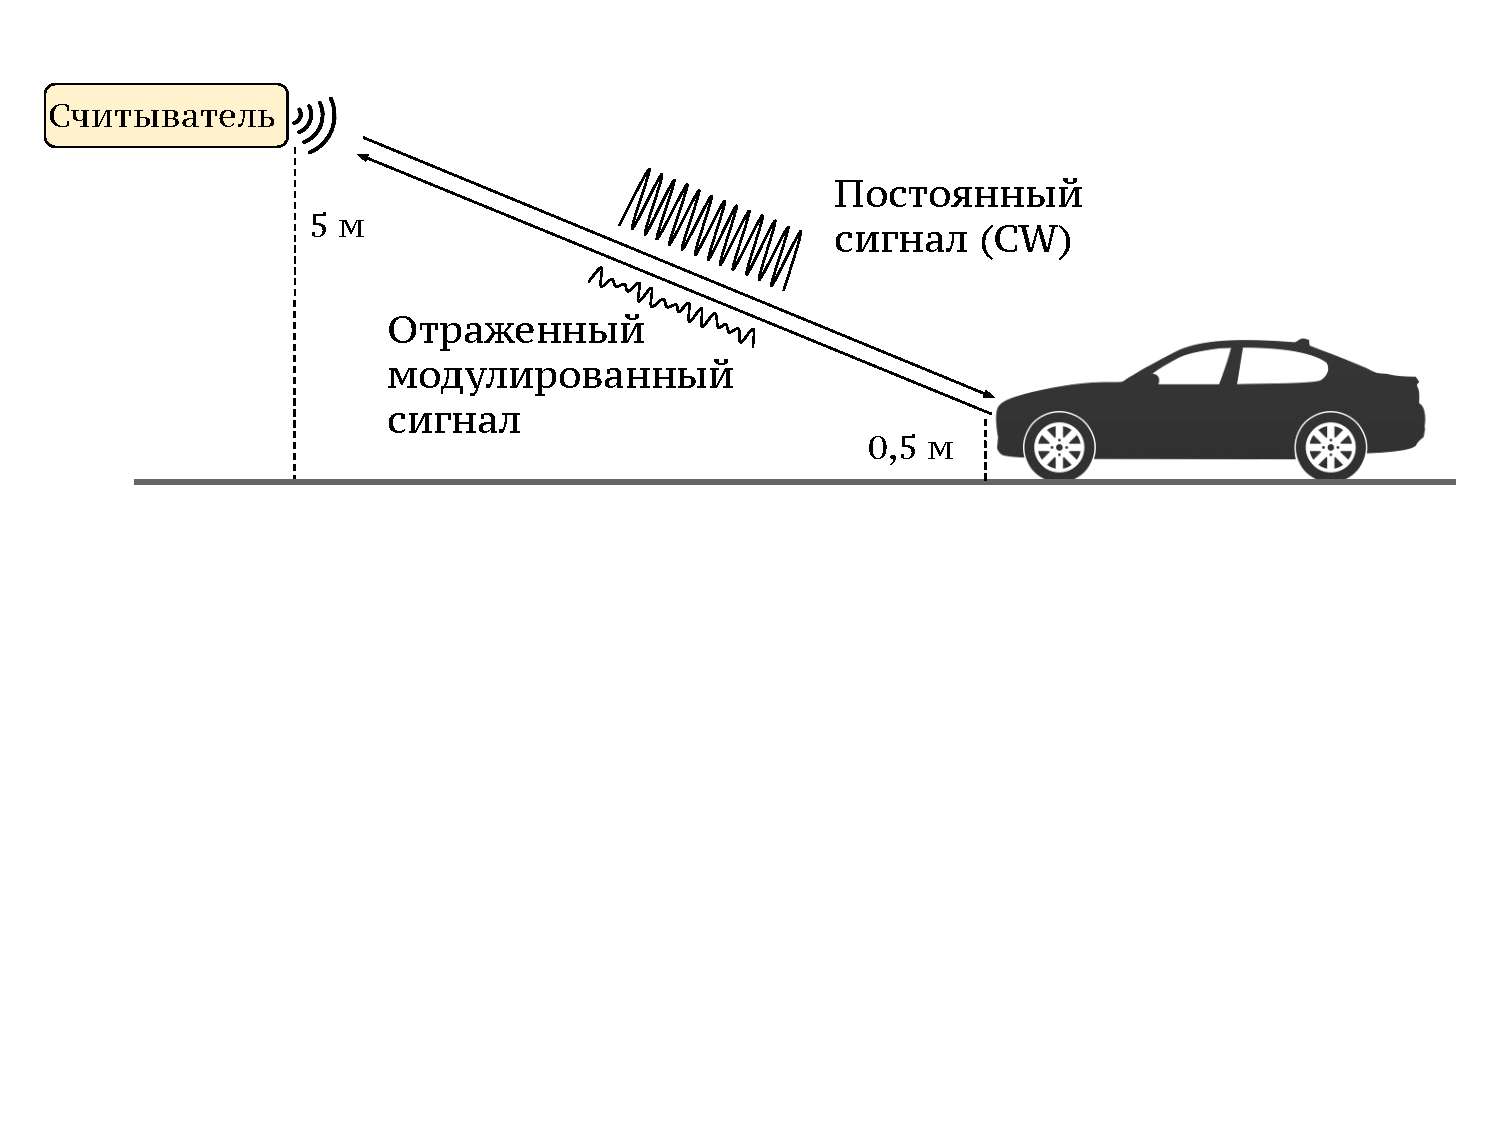
\includegraphics [scale=0.5] {chapter2/ch2_system_structure}
  }
  \caption{Структура системы радиочастотной идентификации автомобилей}
  \label{fig:ch2_system_structure}
\end{figure}

Метки могут размещаться на регистрационных номерных знаках, под лобовым стеклом или на корпусе автомобиля. В настоящей работе рассматривается случай, когда метки расположены на номерах, поскольку этот вариант был использован в проведенном в г. Казань эксперименте. Кроме того, размещение меток в номерных знаках обладает рядом преимуществ: расположение знаков относительно дорожного полотна варьируется в малых пределах, зона номерного знака не загорожена никакими проводящими поверхностями, наконец это решение можно в дальнейшем легко стандартизировать и масштабировать за счет монтирования меток в выпускаемые номерные знаки.

RFID-считыватель размещается над дорогой (например, на тех же опорах, на которых сегодня размещаются камеры), на высоте приблизительно 5 метров; считыватель может оснащаться от 1 до 4 антенн. Таким образом, один считыватель может читать метки в передних и задних номерах на двухполосной дороге.

Связь между меткой и считывателем возможна при соблюдении двух условий: метка получает достаточно энергии для работы и декодирования команд от считывателя (чувствительность современных меток имеет порядок -18 дБм), и отраженный модулированный меткой сигнал поступает на считыватель на достаточно высокой мощности, чтобы быть успешно распознанным и декодированным (при отсутствии коллизий, уровень принимаемого сигнала для современных считывателей должен быть не ниже минус 80 дБм). На практике это означает, что дальность связи составляет порядка 8 -- 15 метров. Однако, из-за особенностей распространения сигнала вблизи автодороги, область, в которой метка может получить достаточно энергии, может иметь достаточно сложный вид и состоять из нескольких непересекающихся областей, общая ширина которых может составлять 2 -- 3 метра. Подробнее эти эффекты будут рассмотрены в последующих разделах.



%%%%%%%%%%%%%%%%%%%%%%%%%%%%%%%%%%%%%%%%%%%%%%%%%%%%%%%%%%%%%%%%%%%%%%%%%%%%%%%%
\section{Общая схема расчёта вероятности идентификации автомобилей}\label{sec:ch2_general_scheme}
%%%%%%%%%%%%%%%%%%%%%%%%%%%%%%%%%%%%%%%%%%%%%%%%%%%%%%%%%%%%%%%%%%%%%%%%%%%%%%%%
Производительность системы определяется как доля успешно идентифицированных автомобилей. Полагая, что успешного чтения хотя бы одной метки достаточно для идентификации автомобиля, вероятность идентификации можно описать следующим образом:

$$
	\mathbb{P}\{A_x\} = 1 - \prod\limits_{\forall t \in  \mathfrak{T}_x} (1 - \mathbb{P}\{A_t\}),
$$
где $A_x$ "--- событие идентификации автомобиля $x$, $A_t$ "--- событие идентификации метки $t$, а $\mathfrak{T}_x$ есть множество меток, размещенных на автомобиле $x$. Вероятность идентификации метки $\mathbb{P}\{A_t\}$ зависит от длительности раунда инвентаризации, вероятности успешной передачи ответа и числа меток в области чтения:

$$
	\mathbb{P}\{A_t\} = 1 - (1 - (1 - \mathbb{P}\{A_c\})\mathbb{P}\{A_r\})^{N_r},
$$
где $A_c$ "--- событие возникновения коллизии, $A_r$ "--- событие успешной передачи меткой ее идентификатора и $N_r$ "--- число раундов, в которых метка успевает принять участие.

Пусть $N_t$ "--- число меток в области чтения и $Q$ "--- параметр антиколлизионного протокола. \cite{StdGen2}. Тогда вероятность возникновения коллизии для данной метки определяется следующей формулой:

$$
	\mathbb{P}\{A_c\} = 1 - (1 - 2^{-Q})^{|N_t| - 1}.
$$

Число раундов можно грубо оценить как:

$$
	N_r \approx \frac{L}{v}\cdot\frac{1}{\tau},
$$
где $L$ "--- общая длина участка дороги с хорошими условиями для чтения (т.е. на этом участке метка получает достаточно энергии для работы и битовая ошибка достаточно низка), $\tau$ "--- средняя длина раунда при заданном числе меток и параметрах протокола, $v$ "--- скорость движения метки. В действительности количество раундов представлеяет собой случайную величину, зависящую от множества параметров, включая количество меток в области чтения, настройки протокола, непосредственный выбор метками слотов для ответов (определяет количество коллизий, пустых слотов и слотов с ответами). Также число раундов зависит от результатов попыток передачи меткой её идентификатора, а также от того, сбрасывал ли считыватель питание между раундами "--- влияние этих факторов оказывается очень существенным и исследуется подробнее в следующей главе диссертации.

Согласно \cite{Nikitin2008}, при отсутствии коллизий основным источником ошибок при расчете $\mathbb{P}\{A_r\}$ является высокий BER при приеме ответов от меток. Пусть $r$ "--- ответ метки, $\mathfrak{R}$ "--- множество всех ответов метки, передача которых необходима для успешной идентификации. Обозначая битовую длину ответа как $|r|$, вероятность успешной передачи всех ответов $\mathbb{P}\{A_r\}$ метки можно вычислить по формуле:

$$
	\mathbb{P}\{A_r\}=\prod_{r \in \mathfrak{R}}(1-B)^{|r|}.
$$

Множество $\mathfrak{R}$ обязательно содержит ответ RN16 на команду, с которой начался слот, в котором метка передаёт ответ (Query, QueryRep или QueryAdjust) и ответ на команду ACK (PC+EPC+CRC). Если для идентификации метки также используется 64-битное значение из банка TID, то $\mathfrak{R}$ также включает ответы на Req\_RN и Read.

Из приведенных формул видно, что для максимизации вероятности идентификации автомобиля необходимо увеличивать вероятность успешной передачи меткой ответов и число раундов, и одновременно уменьшать вероятность коллизий. Однако эти требования вступают в противоречие: более низкий BER достигается при более надежных и медленных настройках протокола, а вероятность коллизии снижается при росте числа слотов, но все это ведет к увеличению длительности раунда. В последующих разделах будет разработан комплекс моделей, позволяющий проанализировать вероятность идентификации метки при различных допущениях, а в конце главы будут приведены результаты расчета вероятности идентификации автомобиля при различных настройках протокола и скорости движения, полученные с помощью детализированной имитационной модели.







%%%%%%%%%%%%%%%%%%%%%%%%%%%%%%%%%%%%%%%%%%%%%%%%%%%%%%%%%%%%%%%%%%%%%%%%%%%%%%%%
\section{Анализ влияния параметров протокола на длительности раундов}\label{sec:ch2_durations}
%%%%%%%%%%%%%%%%%%%%%%%%%%%%%%%%%%%%%%%%%%%%%%%%%%%%%%%%%%%%%%%%%%%%%%%%%%%%%%%%
Считыватель использует модуляции DSB-ASK, SSB-ASK и PR-ASK, а в качестве схемы кодирования используется PIE. Из-за использования PIE (Pulse Interval Encoding) длительность передачи команды зависит от её содержания, так как длительности символов data\_0 и data\_1 отличаются в 1,5--2 раза. Перед каждой командой Query считыватель передает преамбулу, а перед остальными "--- более короткую синхронизирующую последовательность.

\begin{figure}[h]
	\centerfloat{
	  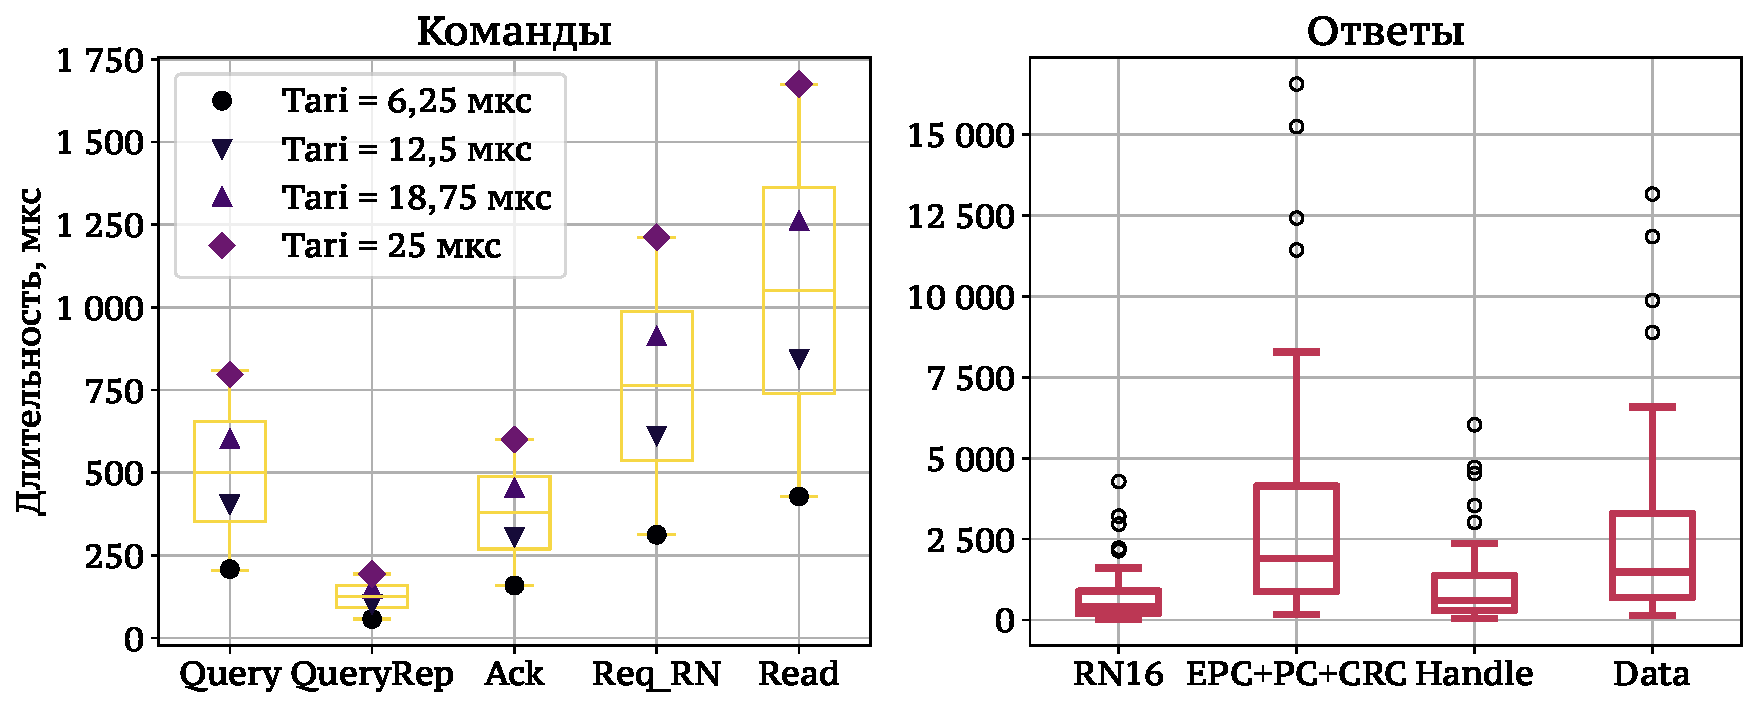
\includegraphics[width=0.9\textwidth]{chapter2/ch2_messages_durations}
	}
	\caption{Разброс длительностей сообщений между считывателем и меткой.}
	\label{fig:ch2_messages_durations}
\end{figure}

На рис.~\ref{fig:ch2_messages_durations} показан разброс длительностей команд считывателя и ответов меток для разных настроек протокола. Длительности команд могут различаться в четыре раза, так как все символы, передаваемые считывателем, пропорциональны длительности Tari. В действительности разброс длительностей команд еще больше "--- при построении графика предполагалось, что отношение длительностей RTcal, TRcal и Tari фиксировано ($\text{RTcal} = 2,75\;\text{Tari}$, $\text{TRcal} = 2,05\;\text{RTcal}$), а стандарт определяет их в диапазоне $2,5\;\text{Tari} \leqslant \text{RTcal} \leqslant 3\;\text{Tari}$ и $1,1\;\text{RTcal} \leqslant \text{TRcal} \leqslant 3\;\text{RTcal}$.

\begin{figure}[h]
	\centerfloat{
	  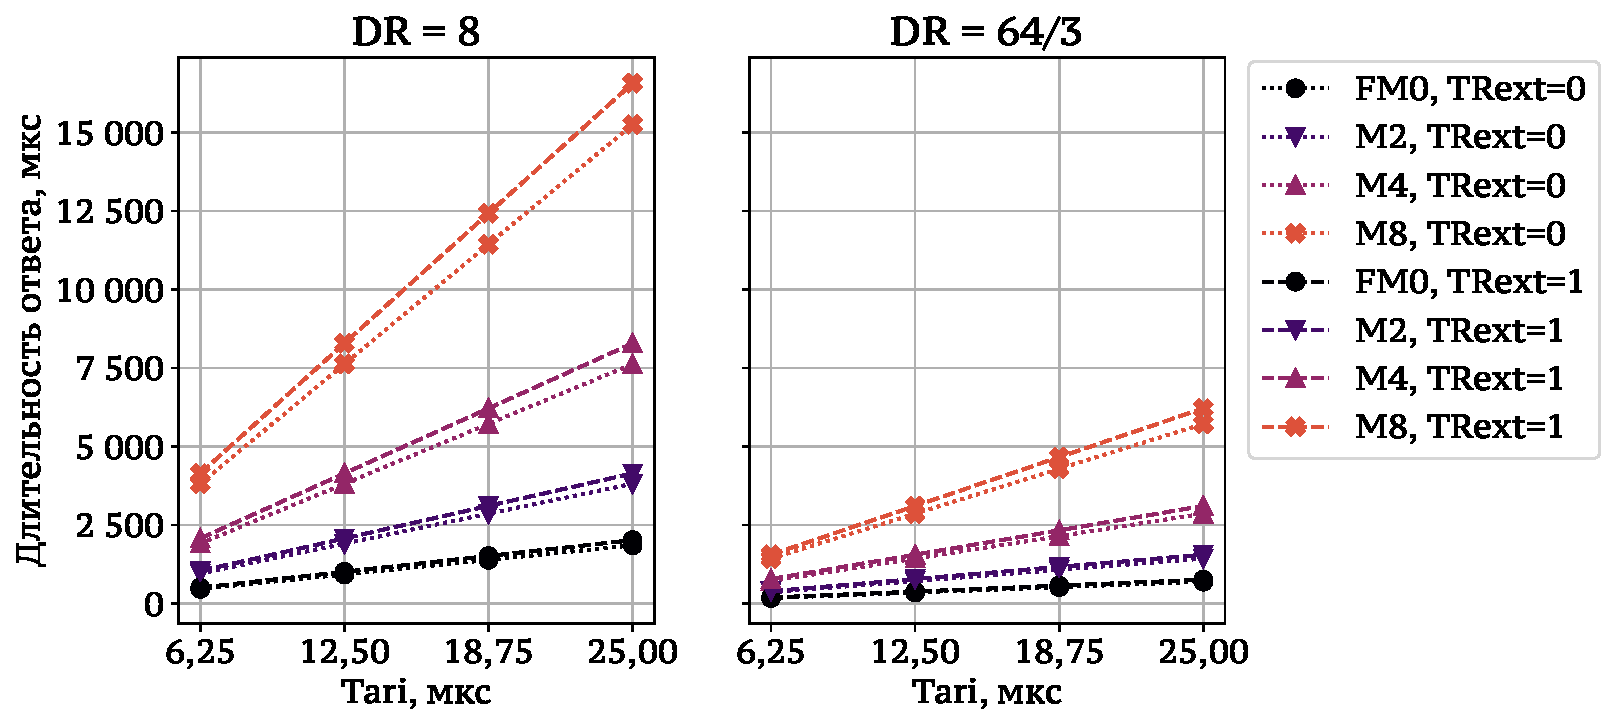
\includegraphics[width=0.9\textwidth]{chapter2/ch2_response_durations}
	}
	\caption{Зависимость длительностей ответов EPC+PC+CRC от параметров протокола.}
	\label{fig:ch2_response_durations}
\end{figure}

Разброс длительностей ответов меток даже больше, чем разброс длительностей команд. Это обусловлено тем, что длительности ответов зависят не только от Tari, но и от параметра DR, способа кодирования ответа (1, 2, 4 или 8 символов на бит) и того, используется ли расширешнная преамбула. На рис.~\ref{fig:ch2_response_durations} показаны зависимости длительностей ответов меток с передачей EPCID, PC и CRC от различных параметров протокола, полученные при фиксированном отношении Tari, RTcal и TRcal. Можно видеть, что, длительность ответа может меняться на два порядка.

При идентификации метки может использоваться только EPCID или комбинация EPCID и значений из других банков, например "--- TID. Первый вариант менее надежен, однако существенно быстрее второго "--- на чтение банков памяти требуется значительно больше времени, так как при этом необходимо осуществить дополнительный обмен сообщениями. На длительность идентификации также влияет, например, использование команды Select для настройки флагов меток и выбора подмножества меток для опроса. В дальнейшем будем рассматривать два самых простых сценария: идентификацию меток только по EPCID (в этом случае взаимодействие ограничивается инвентаризацией) и по комбинации EPCID + TID. Кроме того, будем предполагать, что считыватель не использует команды QueryAdjust и не изменяет выбранное значение параметра Q.

\begin{figure}[!t]
	\centerfloat{
	  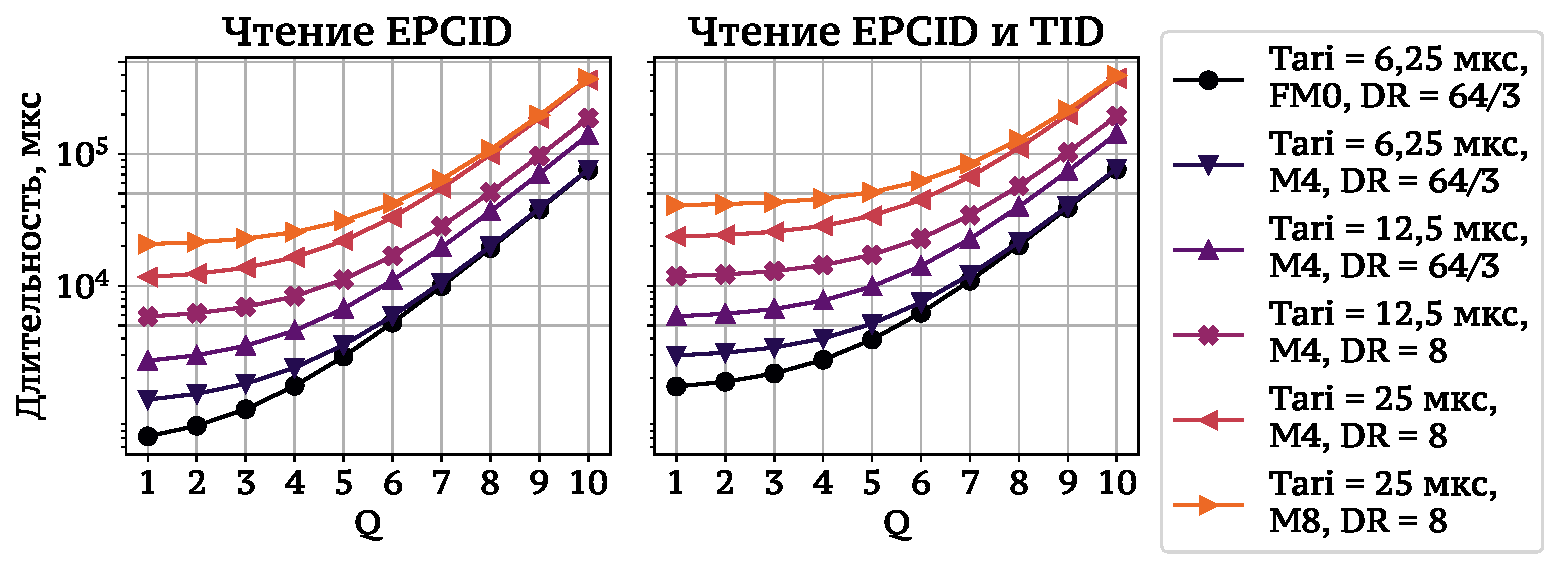
\includegraphics[width=0.9\textwidth]{chapter2/ch2_round_durations}
	}
	\caption{Зависимость максимальной длительности раунда от значения Q.}
	\label{fig:ch2_round_durations}
\end{figure}


Из-за ошибок при передаче ответов, в общем случае метке может потребоваться несколько попыток для передачи своего идентификатора. Максимальное число раундов, в которых может принять участие метка, ограничено областью, в которой она получает достаточно энергии, и скоростью ее движения. Более подробно число раундов, с учетом коллизий и ошибок, анализируется в главе 3, а сейчас рассмотрим простейший модельный случай, когда в раунде передачу ведет единственная метка, и ей удается передать все свои сообщения. То есть в раунде нет коллизий, а ошибки при передаче ответов если и происходят, то только на последних ответах. Длительность раунда $\tau$ для этого модельного случая можно рассчитать по формуле (см. рис.~\ref{fig:ch1_inventory}):

$$
	\tau = t_1 + (2^Q - 1) t_0,
$$
где
$$
	\begin{aligned}
		&t_0 = T_{\text{QueryRep}} + T_1 + T_3\;\text{ "--- пустой слот};\\
		&t_1 = \begin{cases}
			t_1^{\text{(epc)}} &\text{ "--- слот с ответом при идентификации по EPCID};\\
			t_1^{\text{(tid)}} &\text{ "--- слот с ответом при идентификации по EPCID и TID};
		\end{cases}\\
		&t_1^{\text{(epc)}} = T_{\text{Query}} + 2 * (T_1 + T_2) + T_{\text{RN16}} +
			T_{\text{ACK}} + T_{\text{EPCID}};\\
		&t_1^{\text{(tid)}} = t_1^{\text{(epc)}} + 2 * (T_1 + T_2) + T_{\text{Req\_RN}} +
			T_{\text{Handle} + T_{\text{Read}}} + T_{\text{Data}}.
	\end{aligned}
$$
Здесь $T_1$ "--- интервал между концом команды и началом ответа, $T_2$ "--- интервал между концом ответа и следующей командой, $T_3$ "--- интервал между окончанием $T_1$ и новой командой (ожидание ответа), а $T_{\text{msg}}$ "--- длительность команды или ответа msg. Для простоты не учитываем задержку распространения сигнала, которая из-за небольшого расстояния крайне мала. На рис.~\ref{fig:ch2_round_durations} показаны зависимости длительностей раундов, рассчитанные по этим формулам, от значения Tari и величины Q.

\begin{figure}[h]
	\centerfloat{
		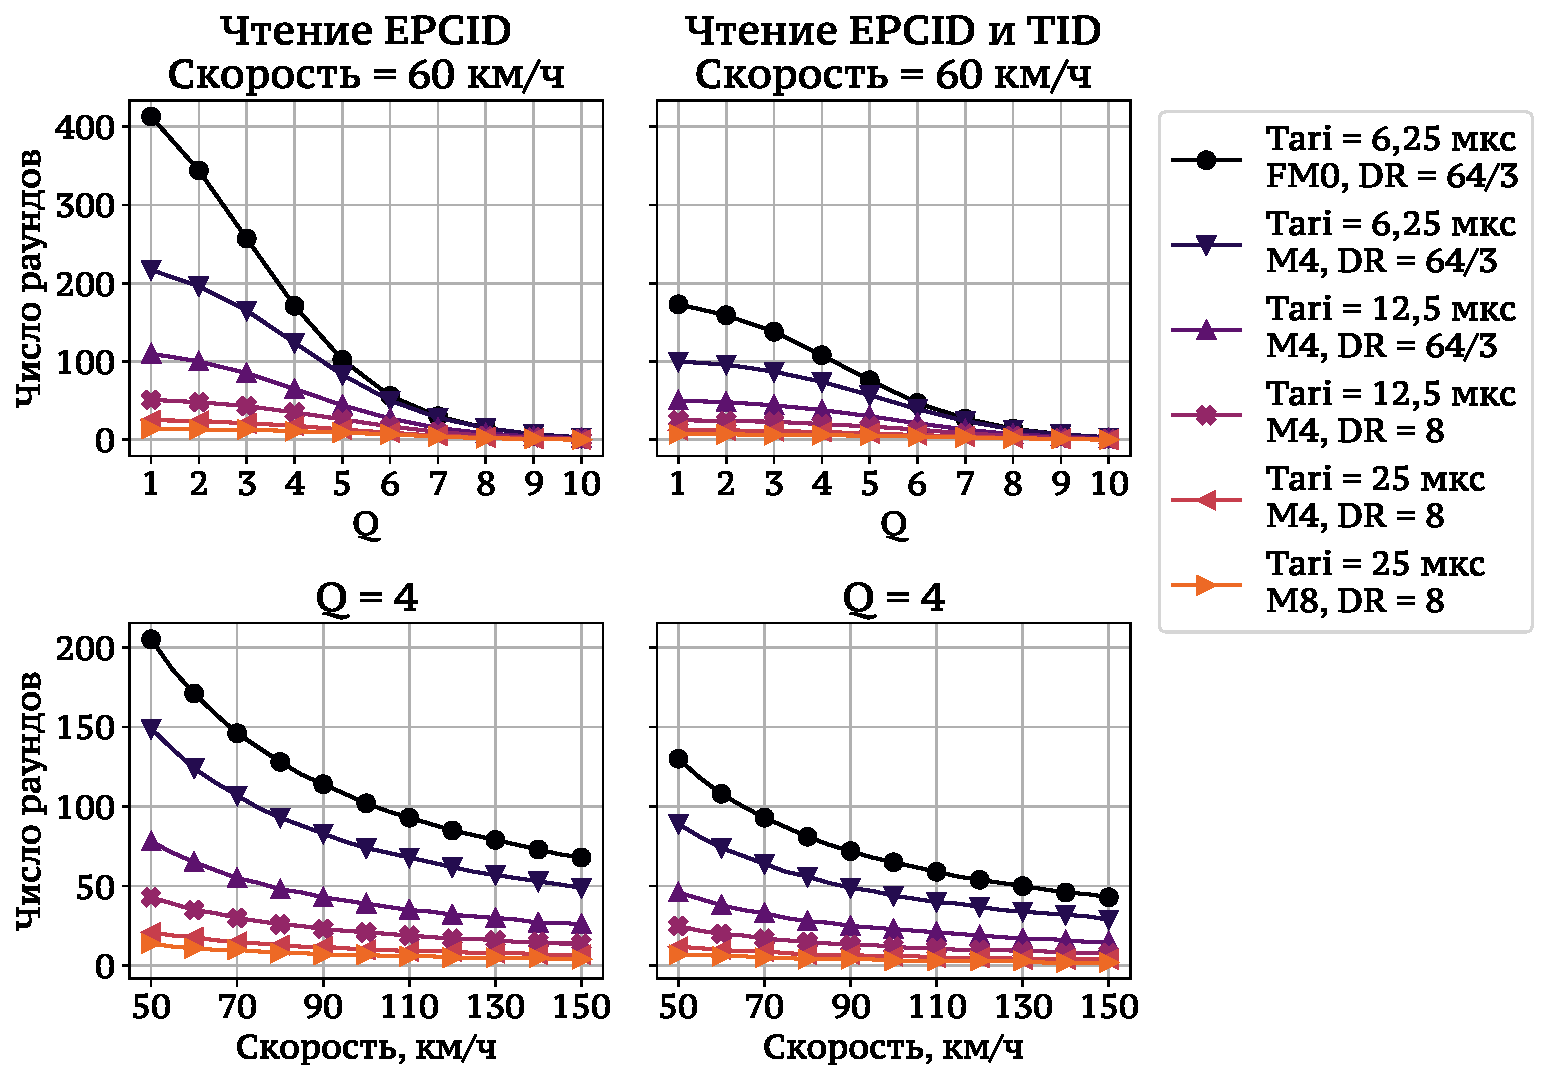
\includegraphics[width=0.9\textwidth]{chapter2/ch2_max_num_rounds.pdf}
	}
	\caption{Зависимость максимального числа раундов, в которых принимает участние метка, от значения Q.}
	\label{fig:ch2_max_num_rounds}
\end{figure}

Зная длительность раунда, скорость движения метки $v$ и размер $L$ области, в которой метка получает достаточно энергии, можно рассчитать максимальное число раундов, в которых метка может передать свой идентификатор, как $N_r \approx \lfloor L / (\tau v) \rfloor$. На рис.~\ref{fig:ch2_max_num_rounds} показана зависимость максимального числа раундов при $L = 5$~метров от значения Q при $v = 60$~км/ч, а также от скорости при $Q = 4$. При увеличении Q и росте скорости число раундов значительно снижается, причем тем быстрее, чем больше Tari и M. В действительности число раундов будет еще меньше из-за переключения считывателя между антеннами, сбросах питания и возможного наличия других меток. Кроме того, метки, ошибшиеся при передаче EPCID и не полуившие после этого команды NACK, не смогут принять участие в следующих раундах, если опрос будет проходить в той же сессии по тому же флагу. Более подробно эти вопросы будут исследованы в следующей главе.




%%%%%%%%%%%%%%%%%%%%%%%%%%%%%%%%%%%%%%%%%%%%%%%%%%%%%%%%%%%%%%%%%%%%%%%%%%%%%%%%
\section{Моделирование радиоканала между считывателем и меткой}\label{sec:ch2_channel}
%%%%%%%%%%%%%%%%%%%%%%%%%%%%%%%%%%%%%%%%%%%%%%%%%%%%%%%%%%%%%%%%%%%%%%%%%%%%%%%%
Для передачи данных от метки используется модуляция обратного рассеяния, метка (не оснащенная источником питания) не может усилить отраженный сигнал. Из-за этого мощность сигнала, принятого на стороне считывателя, значительно ниже, чем мощность на стороне метки. По этой причине битовая ошибка (BER) оказывается выше на стороне считывателя, то есть ошибки с гораздо большей вероятностью появляются при приеме ответов от метки, чем команд от считывателя. Значение BER на стороне считывателя оказывает существенное влияние на успешность чтения меток, поэтому это значение должно быть аккуратно рассчитано.

Для анализа BER рассчитаем бюджет соединения и полуичм значение сигнал--шум (SNR). Результаты этого расчета для стационарного считывателя и метки, размещенной на переднем номере автомобиля, двигающегося со скоростью 60~км/ч, приведены на рис.~\ref{fig:ch2_link_budget}. На горизонтальной оси всех графиков показано расстояние между передатчиком и приемником, на вертикальной "--- время, прошедшее с момента достижения волной приемника. Как будет показано далее (см. формулу~\eqref{eq:ch2_pathloss} для вычисления потерь на распространении сигнала), выбор значения скорости движения существенно влияет на скорость изменения величины затухания в заданной точке.

\begin{figure}[h]
  \centerfloat{
    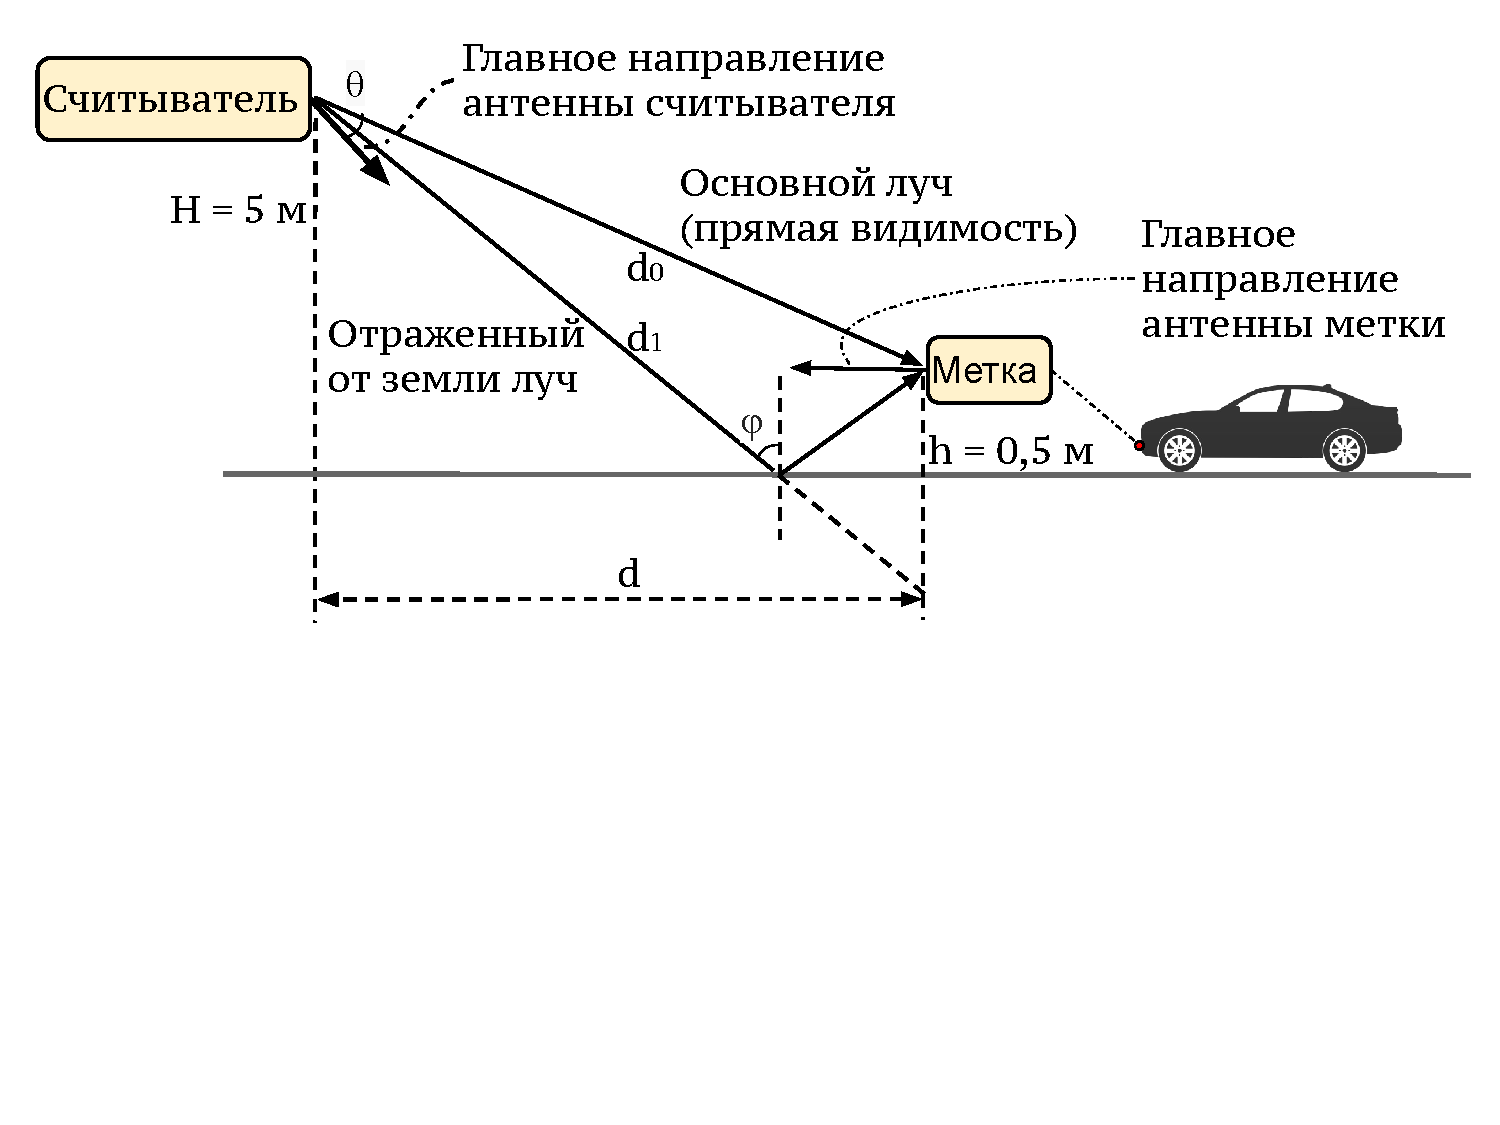
\includegraphics[width=0.8\textwidth]{chapter2/ch2_geometry}
  }
	\caption{Схема системы радиочастотной идентификации автомобилей и ее геометрические параметры}
	\label{fig:ch2_geometry}
\end{figure}



%%% --------------------------------------------
\subsection{Расчёт бюджета соединений}
%%% --------------------------------------------
Пусть $P_t^{(r)}$ "--- излучаемая мощность считывателя, $G^{(r)}$ "--- усиление антенны считывателя. Тогда эффективная изотропная излучаемая мощность (EIRP) составит $EIRP =  P_t^{(r)} G^{(r)}$. Здесь и далее надстрочный индекс используется для обозначения устройства: (r) для считывателя и (t) для метки; подстрочный индекс используется для обозначения направления передачи (прием или передача сигнала). При распространении сигнала от считывателя к метке сигнал испытывает затухание $A_{pl}^{(d)}$, зависящее от состояния радиоканала и взаимного расположения считывателя и метки друг относительно друга. Антенны устройств могут иметь различную поляризацию, что ведет к дополнительным потерям $A_{pol}$. Пусть усиление антенны метки равно $G^{(t)}$. Тогда мощность сигнала, принимаемого меткой, равна:

$$
	P_r^{(t)} = P_t^{(r)} G^{(r)} A_{pl}^{(d)} A_{pol} G^{(t)}.
$$

Если эта мощность меньше чувствительности метки $P_s^{(t)}$, то метка не включится и не сможет взаимодействовать со считывателем. В противном случае метка сможет передавать свои ответы за счет модулирования отраженного сигнала, мощность которого будет равна $P_t^{(t)}$. Поскольку при этом возникают дополнительные энергетические потери (например, из-за модуляции), равные $A_{bs}$, то мощность принятого и отраженного сигналов связаны как $P_t^{(t)} = P_r^{(t)} + A_{bs}$.

Для мощности сигнала, принятого от метки считывателем, можно написать следующее соотношение:

$$
	P_r^{(r)} = P_r^{(t)} G^{(t)} A_{bs} A_{pl}^{(r)} A_{pol} G^{(r)}.
$$

В общем случае потери на прямом (от считывателя к метке) и обратном (от метки к считывателю) путях могут отличаться. Это происходит из-за различия в поляризации (обычно на считывателях используются антенны с круговой поляризацией, а на метках "--- с линейной) и, как следствие, в коэффициенте отражения от земли.

\begin{table}[!t]
	\renewcommand{\arraystretch}{1.3}
	\caption{Параметры, использованные при расчете бюджета соединения}
	\label{table:ch2_budget_params}
	\centering
	\begin{tabular}{|c|c|}\hline
		Параметр & Значение \\\hline
		Мощность, излучаемая считывателем, $P_t^{(r)}$ & 31,5~дБм\\
		Усиление антенны считывателя, $G^{(r)}$ & 8~дБи\\
		Усиление антенны метки, $G^{(t)}$ & 2~дБи\\
		Чувствительность метки, $P_s^{(t)}$ & -18~дБм\\
		Потери на поляризации, $A_{pol}$ & -3~дБ\\
		Потери на модуляции на метке, $A_{bs}$ & -10~дБ\\
		Потери в кабеле, $A_{bs}$ & -2~дБ\\
		\hline
	\end{tabular}
\end{table}

В дальнейших расчетах бюджета соединения будут использованы значения, приведенные в таблице~\ref{table:ch2_budget_params}, типичные для оборудования, применяемого в идентификации автомобилей. При расчете также следует учитывать потери в кабеле, соединяющем антенну со считывателем. Далее считается, что антенны считывателя имеют круговую поляризацию, а меток "--- линейную, таким образом потери на поляризации составляют -3~дБ.

\begin{figure}[h]
	\centerfloat{
    	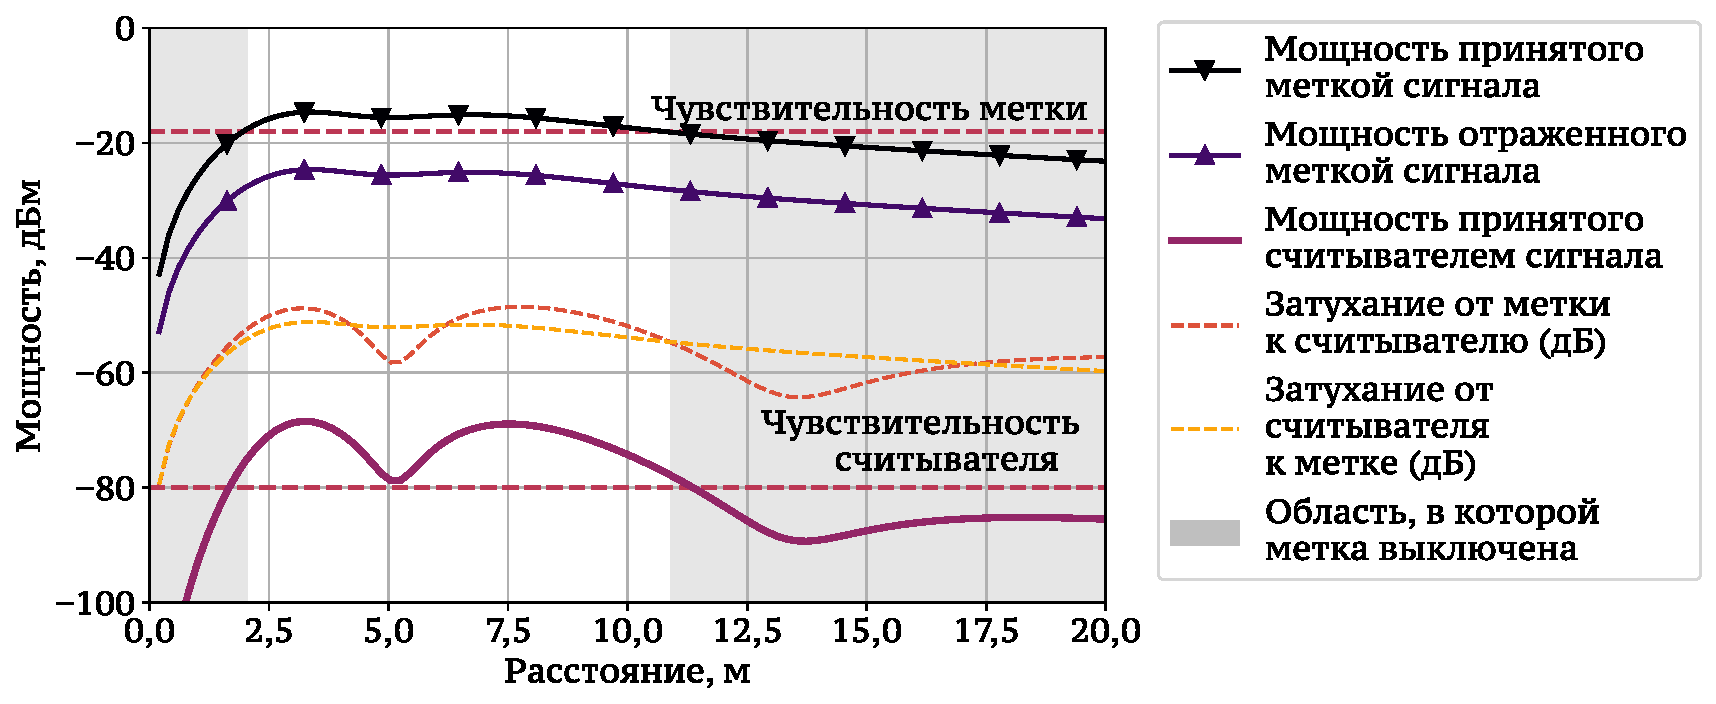
\includegraphics[width=0.85\textwidth]{chapter2/ch2_link_budget}
  	}
	\caption{Расчет бюджета соединения в зависимости от расстояния между считывателем и меткой.}
	\label{fig:ch2_link_budget}
\end{figure}

На рис.~\ref{fig:ch2_link_budget} показан расчет мощностей сигналов, принятых и переданных меткой, принятого считывателем сигнала, а также величина затухания. Все кривые убывают немонотонно из-за изменений с расстоянием в коэффициентах отражения от земли, а также из-за влияния диаграмм направленности антенн. Особенно сильно диаграмма направленности влияет на сигнал при близком расположении метки и считывателя, так как даже небольшое изменение расстояния ведет к ощутимому изменению угла падения. Для того, чтобы связь между расстоянием от считывателя до метки и временем при постоянной скорости оставалась линейной, в качестве расстояния рассматривается дистанция от опоры, на которой размещен считыватель, до метки, измеренная вдоль дороги (см. величину $d$ на рис.~\ref{fig:ch2_geometry}).



%%% --------------------------------------------
\subsection{Расчёт мощности принятых сигналов}
%%% --------------------------------------------

При движении меток и считывателей с ненулевой скоростью друг относительно друга сигналы оказываются подверженными эффекту Доплера, проявляющемуся в сдвиге частоты сигнала на величину, называемую доплеровским сдвигом, и равную:

$$
	\alpha = 1 - \frac{\upsilon \cos{\psi}}{c+\upsilon \cos{\psi}},
$$
где $c$ "--- скорость света, $\upsilon$ "--- скорость приёмника относительно передатчика, в роли приёмника может выступать как метка, так и считыватель (при этом их скорости будут иметь одинаковую величину и противоположные знаки), $\psi$ "--- угол между волновым вектором $\bm{k}$ и направлением движения, $f_c$ "--- несущая частота.

Для узкополосного сигнала в RFID-канале смещённую частоту можно приблизить выражением $\alpha f \approx f - \frac{\upsilon}{c}\cos{\psi} \cdot f_c = f - \nu$, где $\nu$ "--- доплеровский сдвиг:

$$
	\nu = \frac{\upsilon}{c} f_c\cos{\psi} = \frac{1}{2\pi}(\bm{\upsilon},\bm{k}).
$$

При распространении сигнала он может отражаться от дороги, инженерных конструкций, других автомобилей и прочих объектов, то есть в моделируемой системе имеет место многолучевое распространение сигнала. При этом возникает множество копий сигнала $s(t)$, каждая из которых испытывает собственное затухание $h_i$, задержку $\tau_i$ и доплеровский сдвиг $\nu_i$, поскольку каждая копия распространяется по собственному пути, с которым, помимо длины, связаны углы передачи и приема сигнала. Пусть в сигнале присутствует прямая компонента (Line-of-Sight, LoS) сигнала и $N$ отраженных компонент (или лучей). Без потери общности рассуждений будем считать, что LoS-компонента описывается нулевым лучём, а отраженные компоненты "--- лучами $1 \dots N$. Принятый сигнал определяется следующей формулой:

\begin{equation}
	r(t) = \sum\limits_{i=0}^{N} h_i s(t-\tau_i) e^{j\nu_i t}.
	\label{eq:ch2_rx_signal}
\end{equation}

Затухание $h_i$ может быть рассчитано как $h_i=\lambda/(4\pi d_i)R_i\Gamma_i$, где $\lambda$ "--- длина волны, $d_i$ "--- длина пути для $i$--го луча, $R_i$ "--- коэффициент затухания, вызванного отражением сигнала, для $i$--го луча (для основной, LoS-компоненты полагаем равным единице: $R_0=1$), $\Gamma_i = \Gamma_i^{(r)}\Gamma_i^{(t)}$ "--- ослабление сигнала, определяемое диаграммами направленности передающей и принимающей антенн.

Рассмотрим в качестве передаваемого сигнала постоянную волну (синусоидальный сигнал) единичной мощности. После подстановки формул, описанных выше, в выражение для $r(t)$ \eqref{eq:ch2_rx_signal}, получим затухание при распространении сигнала как значение мгновенной мощности на приемнике:

\begin{equation}
	A_{pl} = |r(t)|^2 = \left(\frac{\lambda}{4\pi}\right)^2
		\left|\sum\limits_{i=0}^{N} \frac{R_i\Gamma_i}{d_i}
		e^{-jk(d_i-\upsilon t \cos{\psi_i})}\right|^2.
	\label{eq:ch2_pathloss}
\end{equation}

Расчёт $R_i$, $\Gamma_i$, $d_i$ и $\psi_i$ требует определения путей распространения сигнала по разным лучам. Для статического окружения, при пренебрежении отражениями от движущихся автомобилей, пути могут быть вычислены простыми аналитическими методами. При более сложном динамическом окружении (а также при моделировании отражающих объектов сложной формы) потребуется использовать техники трассировки лучей. Далее, для упрощения расчетов, будем учитывать только две компоненты: прямую (LoS) и отраженную от земли (NLoS) компоненты. Для отраженной NLoS-компоненты коэффициент затухания $R_1$ равен коэффициенту отражения от земли. Далее предполагаем, что антенна считывателя размещена на высоте 5~м, а метки "--- 0,5~м над дорогой. Остальные лучи моделируются нявно, как случайные компоненты,  обуславливающие использование распределение Рэлея при вычислении BER (подробнее об этом "--- в следующем подразделе).

\begin{figure}[h]
	\centerfloat{
    	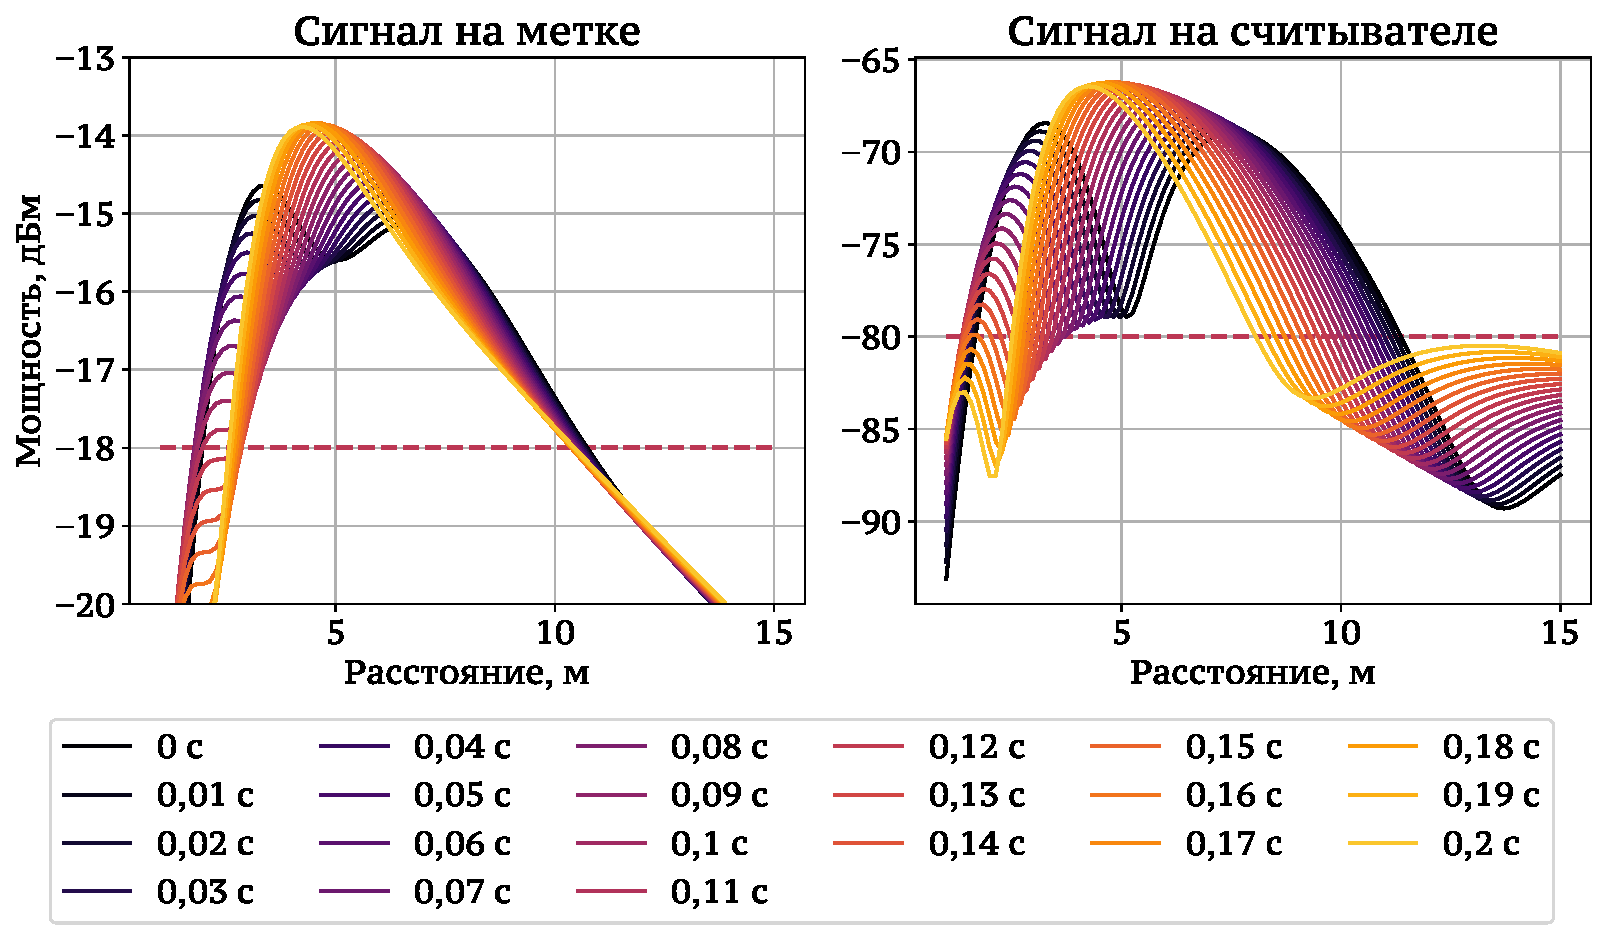
\includegraphics[width=0.85\textwidth]{chapter2/ch2_rx_power_doppler}
	}
	\caption[Зависимость мощности сигналов, принятых меток и считывателем, от расстояния и времени]{Зависимость мощности сигнала, принятого считыватлем, от расстояния между считывателем и меткой $d$ и временем, прошедшим с начала приема меткой сигнала от считывателя}
	\label{fig:ch2_rx_power_doppler}
\end{figure}

Наличие эффекта Доплера делает канал зависимым от времени (см. \cite{Matz2011}), поскольку, как видно из формулы \eqref{eq:ch2_rx_signal}, величина сдвига для каждого луча определяется индивидуально и зависит от времени, прошедшего с начала получения сигнала. Особенность RFID-системы состоит в том, что считыватель не перестает передавать сигнал (постоянный, который метка может модулировать для передачи своего ответа, или информационный) ни после передачи своей команды, ни после получения ответа. Считыватель может прекращать передачу сигнала, например, для сброса флагов сессий меток, при переключении частот или в том случае, если по законодательству он должен периодически освобождать радиоканал. Однако, такие прерывания происходят относительно редко, внутри одного или нескольких раундов сигнал не прерывается. Поэтому значение $t$ в \eqref{eq:ch2_rx_signal} определяется как время, прошедшее со включения считывателя, за вычетом длительности распространения сигнала от считывателя до метки. Хотя метка в это время может еще находиться далеко, радиоканал уже будет существовать. Учитывая, что в момент включения считывателя метки расположены на разных расстояниях от считывателя, получаем, что значение $t$ в одной и той же точке для разных меток будет разным, а соответственно разными будут и значения $r(t)$. На рис.~\ref{fig:ch2_rx_power_doppler} показана зависимость мощностей сигналов, принятых меткой и считывателем, от расстояния $d$, измеренного вдоль дороги. Различные кривые соответствуют времени, прошедшему с начала приема меткой сигнала от считывателя.

\begin{figure}[h]
	\centerfloat{
    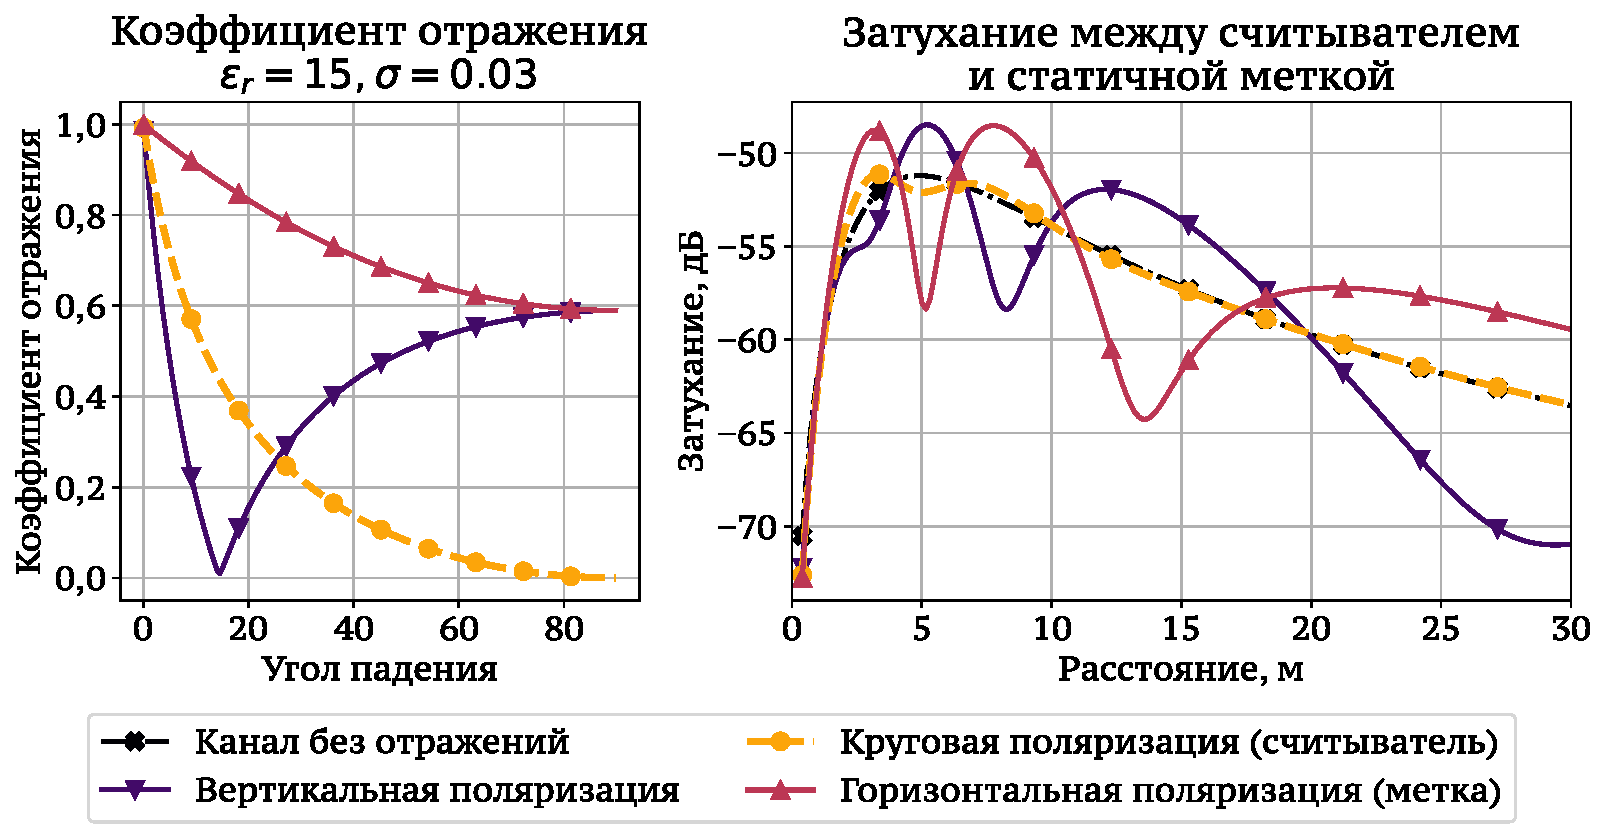
\includegraphics[width=0.85\textwidth]{chapter2/ch2_pathloss}
  }
	\caption{Коэффициент отражения и затухание сигнала для параллельной, перпендикулярной и круговой поляризаций}
	\label{fig:ch2_pathloss}
\end{figure}

На рис.~\ref{fig:ch2_pathloss} показаны результаты расчета затухания сигнала в зависимости от расстояния для разных видов поляризации: параллельной, перпендикулярной и круговой. Различие обусловлено тем, что коэффициент отражения от земли $R_1$ для NLoS-компоненты сигнала принимает разные значения в зависимости от выбранной поляризации. Коэффициент отражения определен следующей формулой \cite{Gonzalez2013}:
$$
  R = \frac{\sin\phi - \sqrt{C}}{\sin\phi + \sqrt{C}},
$$
где $\phi$ "--- угол падения, $C = \eta - \cos^2\phi$ для горизонтально поляризованной компоненты и $C = \frac{\eta - \cos^2\phi}{\eta^2}$ для вертикально поляризованной; $\eta = \epsilon_r(f)-j60\lambda\sigma(f)$, где $\epsilon_r(f)$ "--- относительная диэлектрическая проницаемость поверхности для заданной частоты $f$, $\sigma(f)$ "--- проводимость.

\begin{figure}[h]
	\centerfloat{
    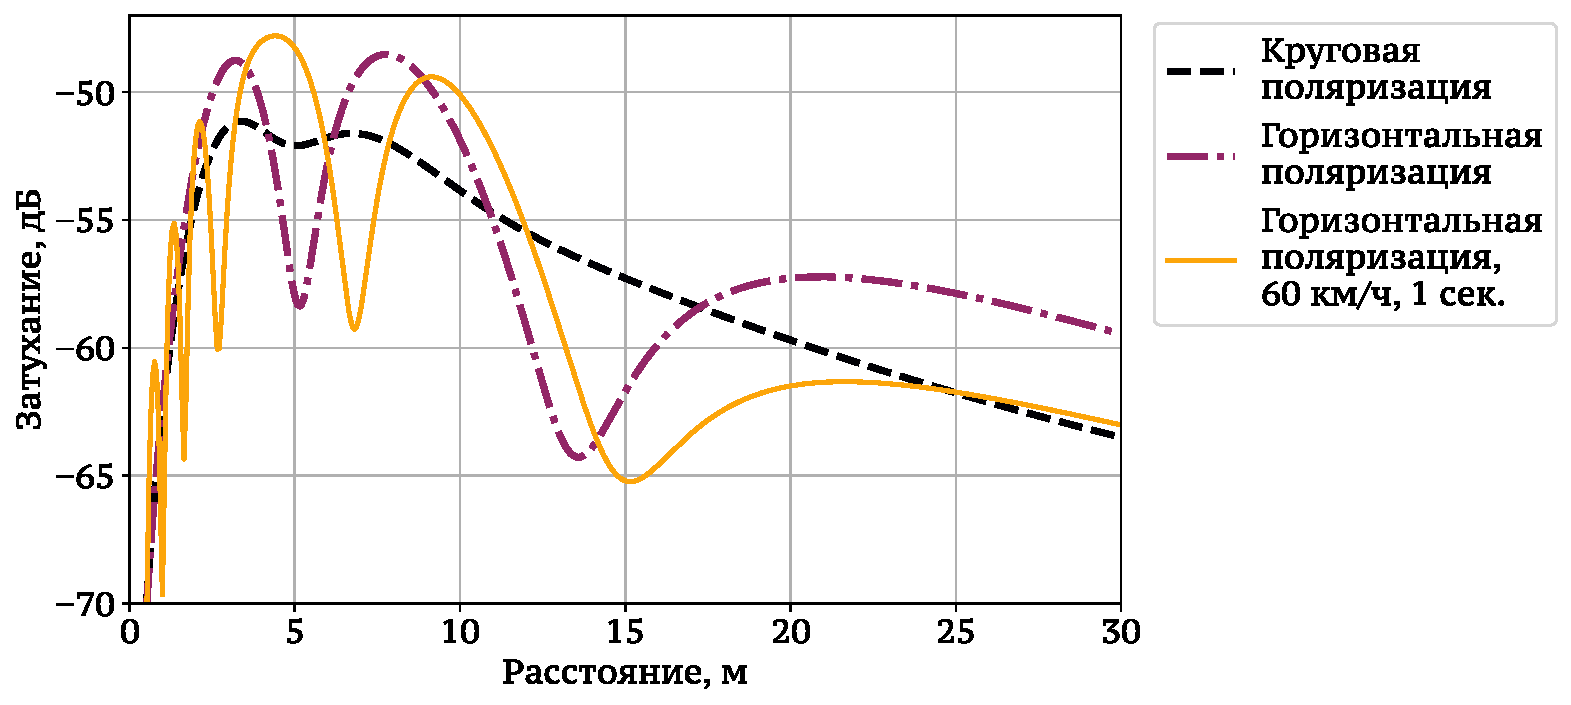
\includegraphics[width=0.85\textwidth]{chapter2/ch2_pathloss_3}
  }
	\caption{Зависимость коэффициента отражения от угла падения для параллельной, перпендикулярной и круговой поляризации при разных значениях относительной диэлектрической проницаемости $\epsilon$ и проводимости $\sigma$.}
	\label{fig:ch2_pathloss_3}
\end{figure}

Относительная диэлектрическая проницаемость и проводимость сильно зависят от влажности поверхности. Проводимость $\sigma$ меняется в диапазоне от 0.00014~См/м для очень сухой земли до 5~См/м для морской воды. Относительная диэлектрическая проницаемость $\epsilon_r$ меняется в диапазоне от 3 до 70. В дальнейшем будем использовать значения проводимости $\sigma = 0,03$~См/м и диэлектрической проницаемости $\epsilon_r = 15$, характерные для сухой дороги с твердым покрытием.

Одновременный учет коэффициента отражения и эффекта Доплера делают зависимость затухания от расстояния достаточно сложной. На рис.~\ref{fig:ch2_pathloss_3} показан пример расчета величины затухания для круговой и горизотнальной поляризаций в момент времени $t = 0$ и через 1 секунду после включения считывателя.

Наконец, для расчета мощностей сигналов необходимо учитывать диаграммы направленности антенн. Будем считать, что у метки простая дипольная антенна, и её диаграмма направленности определяется как:

\begin{equation}\label{eq:ch2_dipole}
	\Gamma(\theta) = \left|
		\frac{\cos{\frac{\pi}{2}\sin{\theta}}}{\cos{\theta}} \right|.
\end{equation}

Для простоты, будем считать, что диаграмма антенны считывателя также определяется с помощью~\eqref{eq:ch2_dipole}. Для более точного расчета можно использовать более подходящие диаграммы, например "--- патч-антенны \cite{Balanis2016}.




%%% --------------------------------------------
\subsection{Расчёт вероятности битовой ошибки (BER)}
%%% --------------------------------------------
\begin{figure}[h]
	\centerfloat{
    	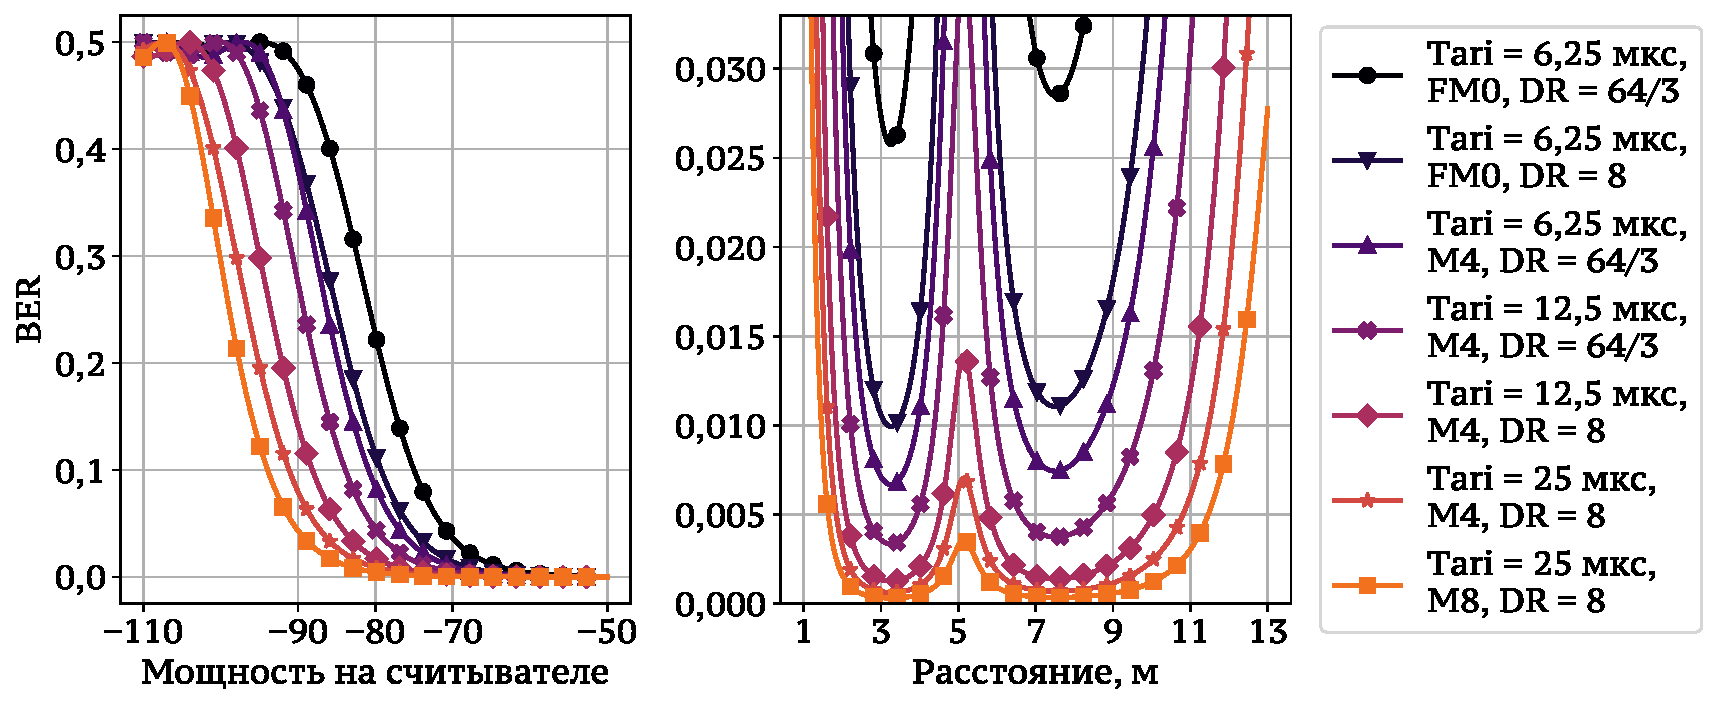
\includegraphics[width=0.9\textwidth]{chapter2/ch2_ber}
  	}
	\caption{Вероятность битовой ошибки (BER) для разных параметров Tari и M}
	\label{fig:ch2_ber}
\end{figure}

Рассмотрим радиоканал с аддитивным гауссовским шумом (AWGN). Вероятность ошибки в передаче бита (BER) можно выразить следующей формулой:

\begin{equation}
	P_{er} = 2Q(\acute{\gamma})[1-Q(\acute{\gamma})],
	\label{eq:ch2_awgn}
\end{equation}
где $Q(\cdot)$ "--- Q--функция; $\acute{\gamma} = mE_s/N_0\cos^2{\phi_s}$; $m$ "--- число символов на бит (порядок) в коде Миллера, $E_s$ "--- энергия одного символа, $N_0/2$ "--- спектральная плотность белого шума и $\phi_s$ "--- разность между реальной и принятой фазами сигнала. Соотношение $E_s/N_0$ может быть выражено как $\gamma T_s B$, где $\gamma$ отношение сигнал-шум (SNR), $T_s$ "--- длительность символа и $B$ "--- ширина полосы. Ошибку синхронизации фазы будем приближенно моделировать как $\cos^2{\phi_s} \approx 1/\gamma T_{pr}B$, где $T_{pr}$ "--- длительность преамбулы \cite{RFID_JRFID2017}.

Использование гауссовской модели оказывается слишком оптимистичным, так как при расчете мощности принятого сигнала учитываются не все лучи. Далее будет использоваться выражением, получаемым усреднением $P_{er}$ в формуле \eqref{eq:ch2_awgn} по $\acute{\gamma}$, которую считаем случайной величиной, имеющей распределение Рэлея \cite{Lazaro2009}:

$$
	P_{er} = \frac{1}{2} - \frac{1}{\sqrt{1+\frac{2}{\acute{\gamma}}}} +
			 \frac{2}{\pi}\frac{\arctan{\sqrt{1+\frac{2}{\acute{\gamma}}}}}{1+\frac{2}{\acute{\gamma}}}.
$$

\begin{figure}[h]
	\centerfloat{
    	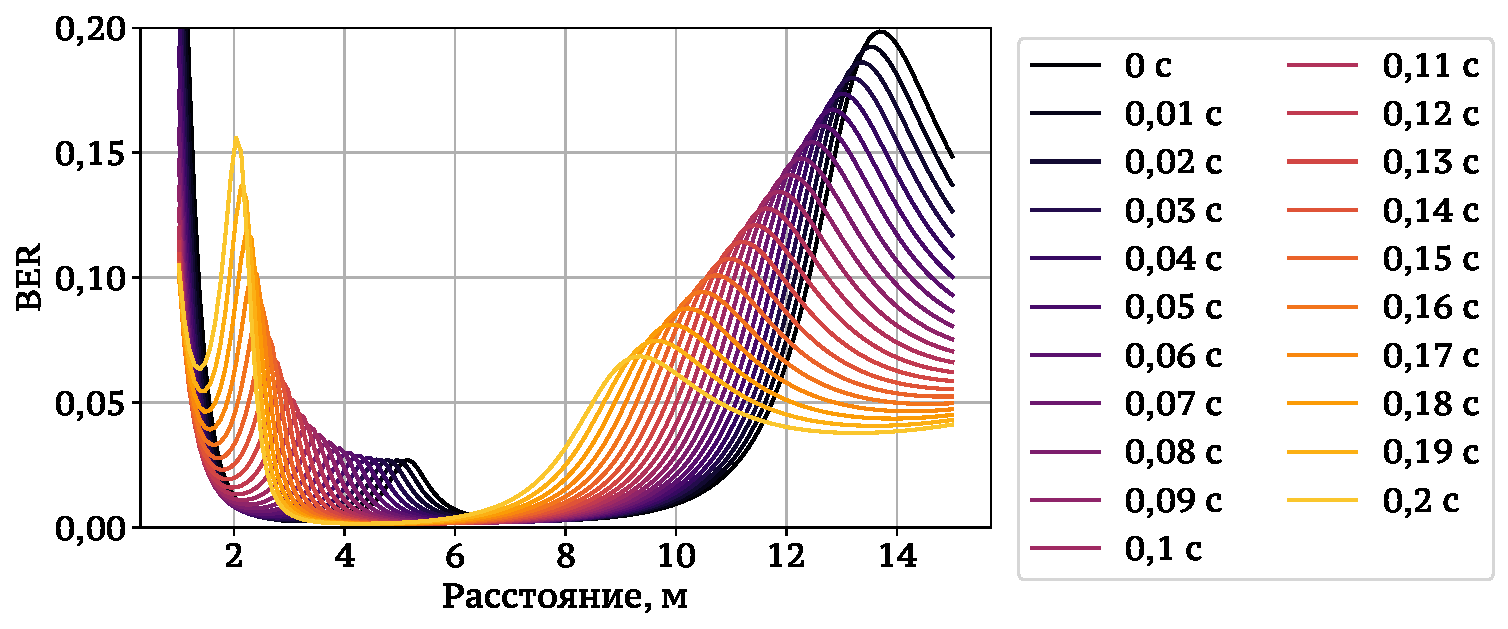
\includegraphics[width=0.8\textwidth]{chapter2/ch2_ber_doppler}
  	}
	\caption{Изменение вероятности битовой ошибки (BER) из-за эффекта Доплера.}
	\label{fig:ch2_ber_doppler}
\end{figure}

На рис.~\ref{fig:ch2_ber} показана зависимость BER от выбранного типа кодирования ответа метки. Как и следовало ожидать, при росте числа символов на бит $m$ и уменьшении BLF (при увеличении Tari и уменьшении DR) BER снижается. Так, при Tari = 6,25~мкс, коде FM0 (m = 1) и DR = 64/3 BER не опускается ниже 0,025, в то время как при Tari = 25 мкс, коде Miller-8 (m = 8) и DR = 8 BER оказывается ниже 0,001 в области размером около 5 метров. При этом число попыток передать свой идентификатор у метки, то есть число раундов, зависит от тех же параметров противоположным образом (см. рис.~\ref{fig:ch2_max_num_rounds}).

Для успешной передачи EPCID метке нужно передать без ошибок RN16 (16 бит) и ответ на ACK, содержащий EPCID, PC (16 бит) и CRC (16 бит). Полагая длину EPCID, равной 96 битам, в общей сложности метка должна передать 144 бита. При BER = 0,01 вероятность успешной передачи составит 23,5\%, при BER = 0,005 "--- 48,8\%, а при BER = 0,001 "--- 86,5\%. Учитывая, что метка может принять участие только в небольшом количестве раундов (см. рис.~\ref{fig:ch2_max_num_rounds}), нужно выбирать такие параметры протокола, при которых область с низким BER будет достаточно большой, и при этом метка должна успеть совершить несколько попыток передачи идентификатора. Отметим, что из-за немонотонной зависимости BER от расстояния, такая область разбивается на <<окна>>, а из-за эффекта Доплера (см. рис.~\ref{fig:ch2_ber_doppler}) эти <<окна>> смещаются с течением времени от включения считывателя.



%%%%%%%%%%%%%%%%%%%%%%%%%%%%%%%%%%%%%%%%%%%%%%%%%%%%%%%%%%%%%%%%%%%%%%%%%%%%%%%%
\section{Результаты имитационного моделирования}\label{sec:ch2_results}
%%%%%%%%%%%%%%%%%%%%%%%%%%%%%%%%%%%%%%%%%%%%%%%%%%%%%%%%%%%%%%%%%%%%%%%%%%%%%%%%
Для проведения численного эксперимента была разработана имитационная модель на языке Python. Исходный код модели, документация и собранные данные можно найти в Git-репозитории на GitHub: \url{https://github.com/larioandr/thesis-rfidsim}.

Разработанная дискретно-событийная имитационная модель "--- достаточно гибкая и простая, позволяет легко вносить изменения для адаптации к другим экспериментам. Состояние модели изменяется при наступлении различных событий "--- начала и окончания приема сигнала, окончания ожидания сообщения, обновления положения меток, таймаута для переключения антенны считывателя, генерации нового автомобиля с меткой и прочих. Для того, чтобы учесть изменение мощностей сигналов при движении метки, затухания и мощности пересчитывались периодически при обновлении положения метки (каждую миллисекунду модельного времени), и записывались для дальнейшего определения минимального уровня сигнала и расчета BER. Более подробное описание модели можно найти в репозитории. Главный недостаток модели "--- высокая вычислительная сложность. Так, для получения численных результатов, представленных в диссертационном исследовании, потребовалось около восьми часов выполнения модели на четырехядерном сервере Модель имеет более 50 параметров, в том числе:
\begin{itemize}
	\item настройки протокола: интервалы Tari, RTcal, TRcal, метод кодирования ответов меток (M), коэффициент DR, использовать ли расширенную преамбулу (TRext);
	\item параметры мобильности меток: скорость движения, частота генерации;
	\item параметры окружения: число и ширина полос движения, длина автомобилей, относительная диэлектрическая проницаемость и проводимость дорожного покрытия, уровень шума;
	\item параметры считывателя: мощность передатчика, потери в кабеле, поляризация, усиление, диаграмма, высота и угол наклона антенн, порядок выбора флагов сессии для опроса;
	\item параметры меток: высота установки, поляризация, усиление и диаграмма антенн, потери на отражении сигнала, длина EPCID и TID, чувствительность;
	\item параметры канала: учиытвать ли эффект Доплера, модель для расчета BER.
\end{itemize}

В ходе численного эксперимента были получены оценки идентификации автомобилей, на которых были установлены RFID-метки. Автомобиль считался идентифицированным, если была успешно прочитана хотя бы одна метка в переднем или заднем номере. Кроме того, для более глубокого понимания работы системы, было исследовано число раундов, в которых успевает принять участие движущаяся метка.



%%% --------------------------------------------
\subsection{Анализ влияния частоты переключений антенн на число раундов}
%%% --------------------------------------------
Точное число раундов, в которых успевает принять участие метка, зависит как от настроек протокола (схема кодирования ответов метки, выбор параметра Q и пр.), так и от алгоритма выбора сессии и частоты смены антенн. Так как вероятность прочитать и EPCID, и TID в одном раунде относительно мала, существенным оказывается то, в скольких раундах метка успевает принять участие, т.е. сколько у нее будет попыток передать свои идентификаторы.

В начале раунда инвентаризации считыватель выбирает сессию (S0, S1, S2, S3) и значение её флага ($A$ или $B$). Метка отвечает только в том случае, если хранимеый ею флаг выбранной сессии совпадает с переданным в команде Query. После рассылки своего EPCID в ответе на ACK, метка инвертирует значение хранимого флага сессии ($A \rightarrow B,\, B \rightarrow A$). Для каждой сессии стандарт определяет интервал времени после выключения питания, в течение котрого метка должна сохранять значение флага сессии, а после которого, если питания так и не появилось, "--- возвращать значение $A$. В дальнейшем будем рассматривать сессию S0, для которой эта процедура самая прстая "--- значение $A$ должно быть установлено сразу после сброса питания, независимо от длительности потери энергии.

\begin{figure}[h]
	\centerfloat{
    	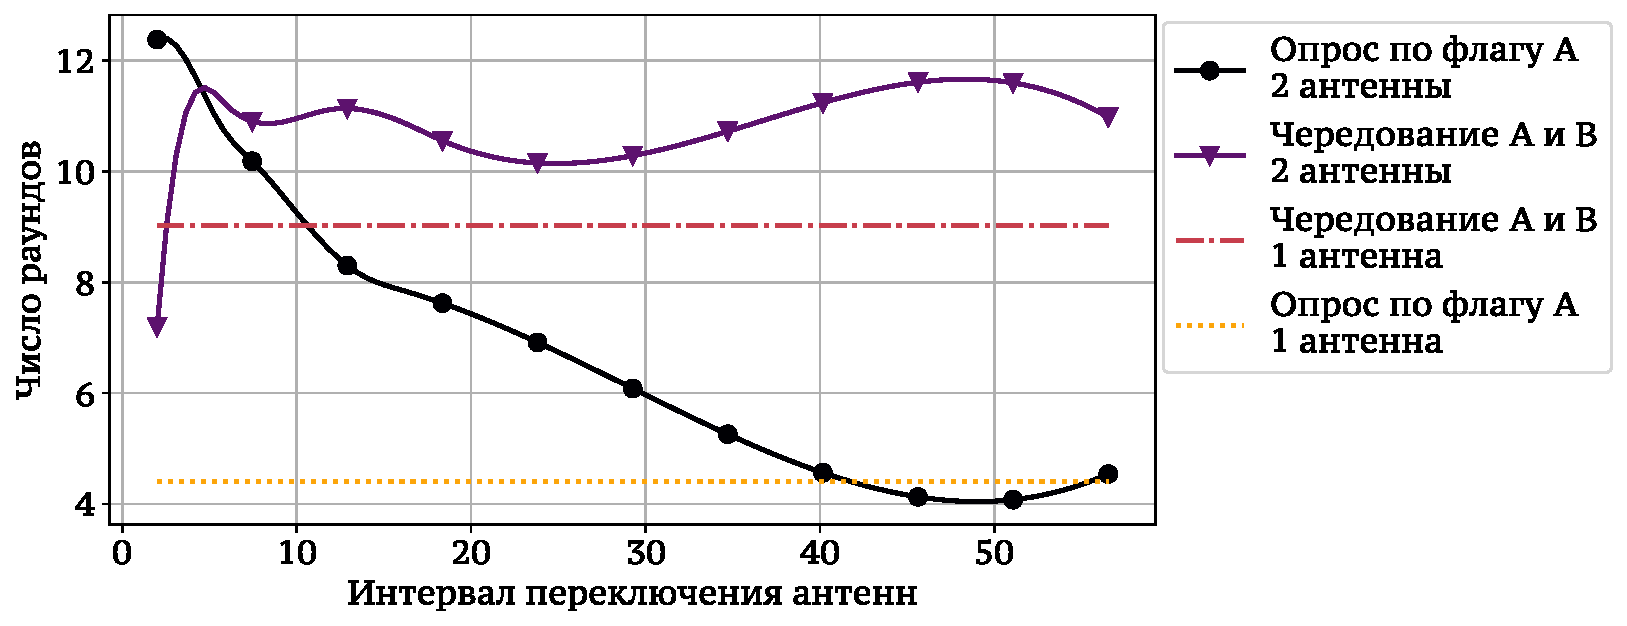
\includegraphics[width=0.8\textwidth]{chapter2/ch2_sim_num_rounds_one_lane}
  	}
	\caption{Число раундов, в которых участвует метка, в зависимости от длительности работы на одной антенне, для разных стратегий выбора флага сессии.}
	\label{fig:ch2_rounds_per_tag}
\end{figure}

Если считыватель использует одну антенну без периодического выключения питания, число раундов, в которых участвует метка, зависит только от стратегии выбора флага сессии. На рис.~\ref{fig:ch2_rounds_per_tag} приведены результаты симуляции, которые показывают, что число раундов при опросе меток только со значением флага сессии S0 = $A$ (самая нижняя горизонтальная линия) и число раундов при смене значений запрашиваемых флагов каждый раунд отличаются в шесть раз. В первом случае число раундов, в которых принимает участие метка, определяется только числом включений метки (выключения обусловлены приемом сигнала считывателя на уровне, меньшем чувствительности метки). При периодической смене флагов метка имеет возможность повторно участвовать в опросе и без выключения, поэтому число раундов оказывается значительно больше, а тем самым повышается вероятность того, что хотя бы один раз метка успешно передаст свои идентификационные данные. Небольшие колебания на приведенном графике обусловлены случайным характером процесса чтения меток, а также случайностью длительности раундов, зависящей от числа занятых и пустых слотов. Также следует отметить, что на число раундов может влиять выбор параметра Q (график соответствует значению Q = 2), а также использование операции Select, которая в представленном исследовании не использовалась.

Если считыватель использует несколько антенн и периодически между ними переключается, число раундов также зависит от интервала между переключениями антенн. На рис.~\ref{fig:ch2_rounds_per_tag} показаны результаты, полученные исходя из того, что считыватель размещен над однополосной дорогой и оборудован двумя антеннами, направленными в противоположные стороны (для чтения переднего и заднего номеров). Можно видеть, что периодическая смена флагов сессии также позволяет увеличить число раундов, хотя и меньше, чем при использовании одной антенны. Можно заметить, что сильнее всего выбор интервала переключения антенн влияет на число раундов при малых значениях интервала. Это связано, в первую очередь, с тем, что при этом переключение происходит каждый раунд или быстрее, метка может не успеть передать свой EPCID до потери энергии (здесь предполагается, что переключение антенн не связано с границами раунда, что является некоторым упрощением). Это связано, в первую очередь, с тем, что периоды работы на одной антенне быстро становятся сопоставимыми с длительностью проезда зон с уровнем сигнала от считывателя, превышающим чувствительность меток. При увличении мощности сигнала или чувствительности меток зависимость должна оказываться более сильной.

Следует отметить, что при использовании других сессий (например, S2), результаты оказываются ближе к случаю отсутствия переключения антенн для малых интервалов, так как при малых интервалах между переключениями (меньших, чем время сохранения флага сессии) метка может <<не заметить>> потерю энергии и сохранить значение флага.

На число раундов также влияет длительность работы считывателя до его выключения и время нахождения в выключенном состоянии. Все расчёты в этом и следующем разделе сделаны в предположении, что считыватель выключается каждые 2 секунды на 100 милисекунд.



%%% --------------------------------------------
\subsection{Анализ вероятности идентификации транспортных средств}
%%% --------------------------------------------
С помощью имитационной модели была изучена вероятность идентификации меток, расположенных на номерах автомобилей, двигающихся по однополосной дороге. Считыватель был оборудован двумя антеннами, размещенными над дорогой в противоположных направлениях, для чтения переднего и заднего знаков.

Для выбора параметра Q было рассчитано среднее число меток, участвующих в одном раунде. Результаты этого расчета приведены в табл.~\ref{table:ch2_tags_num_per_round}, где $N_v$ "--- среднее число автомобилей вблизи считывателя, $T_v$ "--- средний интервал времени между появлениями автомобилей, $N_t$ "--- среднее число меток, участвующих в раунде, а $N_t^{(1)}$ "--- среднее число меток в тех раундах, в которых участвует хотя бы одна метка. Из приведенных результатов видно, что даже при очень интенсивном потоке, когда в зоне действия считывателя оказывается более пяти машин, из-за неравномерности уровня сигнала большая часть меток оказывается выключенными, и можно считать, что в каждом раунде участвует не более одной метки. Фактически это означает, что вероятностью коллизий можно пренебречь и выбирать значение Q сколь угодно малым, так как его увеличение лишь добавит пустых слотов. Учитывая, что длительность пустого слота достаточно мала и для перестраховки на тот случай, когда помимо меток в номерех в зону действия попадут  другие метки (расположенные, например, на предметах под стеклом автомобиля или на самом автомобиле), можно установить Q=2. В дальнейшем это значение будет использовано для получения остальных результатов.

\begin{table}[h]
	\renewcommand{\arraystretch}{1.3}
	\caption{Среднее число меток, участвующих в раунде, при движении автомобилей со скоростью 60~км/ч}
	\label{table:ch2_tags_num_per_round}
	\centering
	\begin{tabular}{|c|c|c|c|}
		\hline
		$T_v$, sec & $N_v$ & $N_t$ & $N_t^{(1)}$ \\\hline
		0.5 & 5.67 & 0.1000 & 1.0 \\\hline
		1.0 & 3.38 & 0.0357 & 1.0 \\\hline
		\end{tabular}
\end{table}


\begin{figure}[h]
  \centerfloat{
    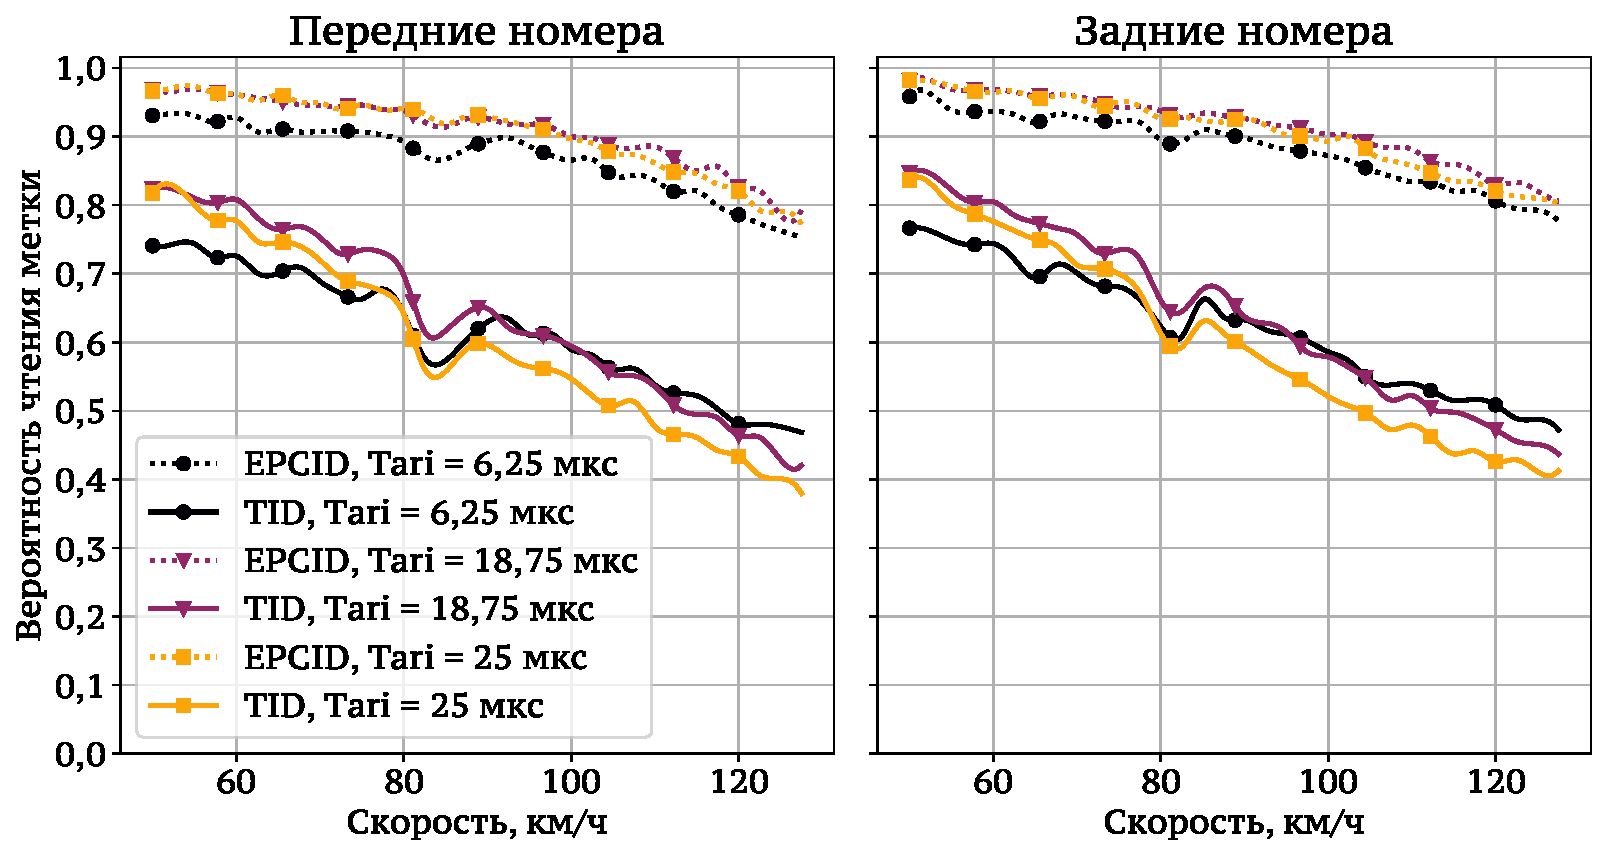
\includegraphics[width=0.9\textwidth]{chapter2/ch2_tag_identification_m4}
  }
	\caption{Вероятность успешного чтения меток в номерах при различных значениях Tari и кодировании ответов M = 4}
	\label{fig:ch2_tag_identification_m4}
\end{figure}

\begin{figure}[h]
  \centerfloat{
    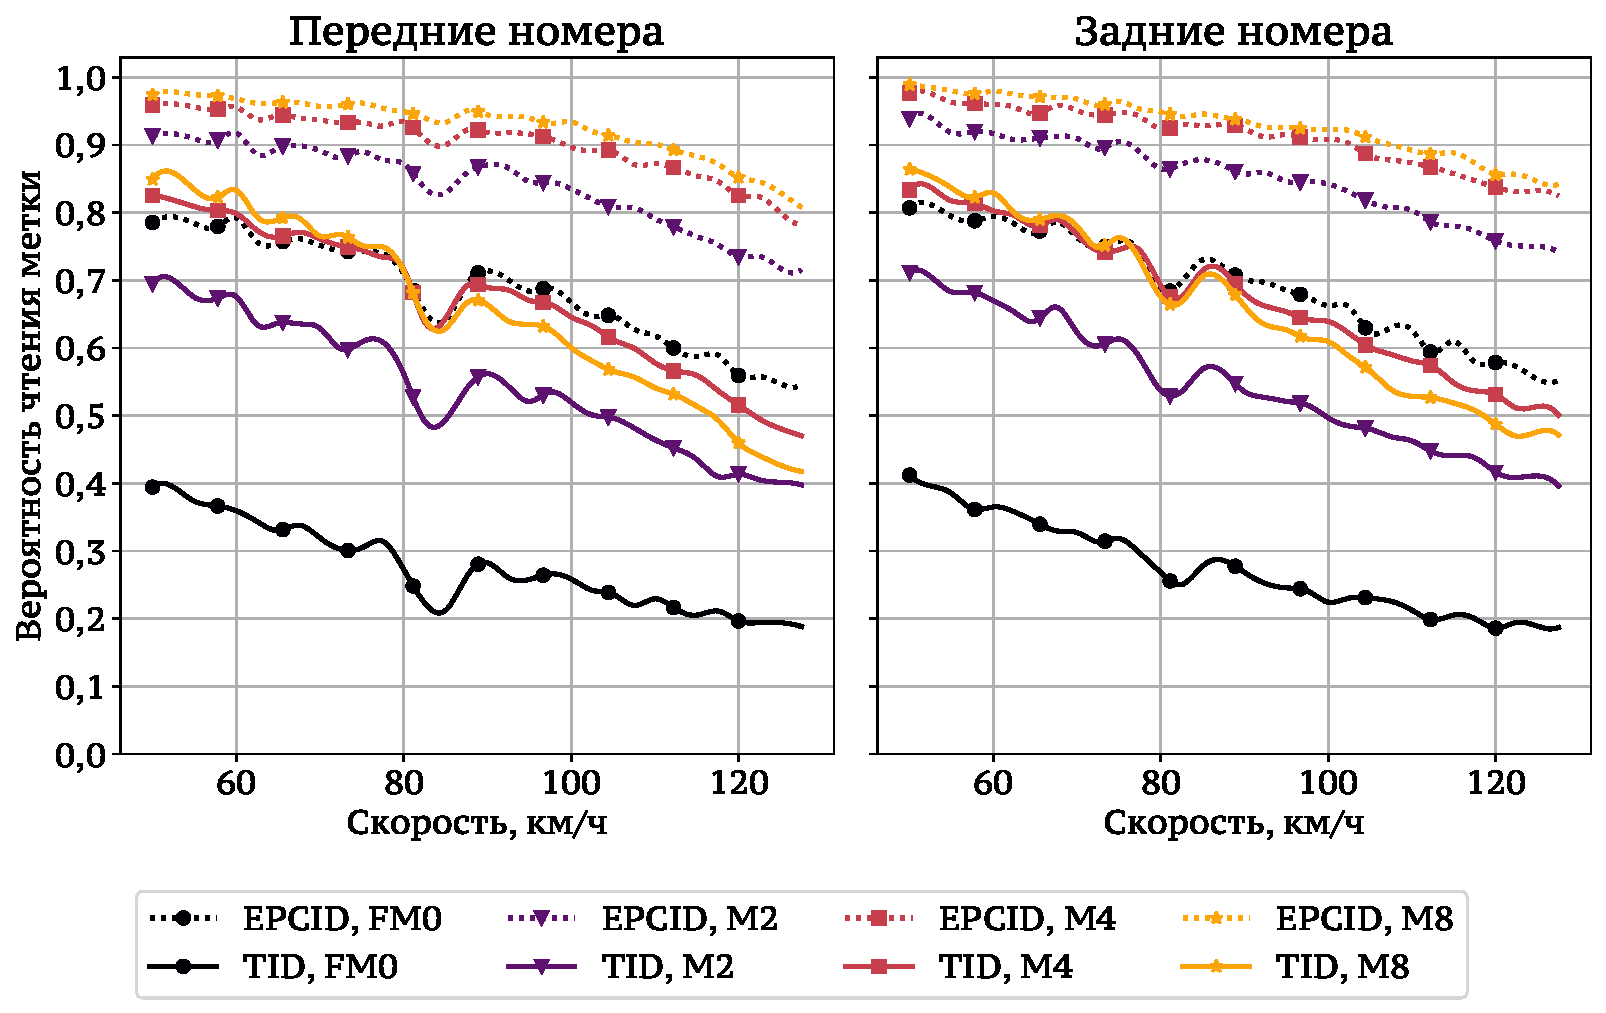
\includegraphics[width=0.9\textwidth]{chapter2/ch2_tag_identification_tari125}
  }
	\caption{Вероятность успешного чтения меток в номерах при различных значениях M и Tari = 12,5~мкс}
	\label{fig:ch2_tag_identification_tari125}
\end{figure}

На рис.~\ref{fig:ch2_tag_identification_m4} и \ref{fig:ch2_tag_identification_tari125} показаны результаты расчёта вероятности идентификации меток в номерах в заивисимости от скорости движения автомобилей при различных значениях интервала Tari (см. рис.~\ref{fig:ch2_tag_identification_m4}) и различных значениях M (число символов на бит в ответах меток, см. рис.~\ref{fig:ch2_tag_identification_tari125}). Предполагалось, что антенны считывателя имеют усиление 8~дБи, потери в кабеле составляют 2~дБ, метки используют расширенные преамбулы, а значение DR=8. Считыватель работал в сессии S0, инвертировал значение флага сессии в каждой команде Query и переключал антенны каждые 100~мс. Из приведенных графиков видно, что вероятность чтения меток падает с ростом скорости. При этом вероятность чтения EPCID остаётся высокой при достаточно больших скоростях свыше 120~км/ч, чего нельзи сказать про чтение TID. Важно отметить, что выбор больших значений Tari не обязательно ведет к увеличению вероятности успешной идентификации (см. рис.~\ref{fig:ch2_tag_identification_m4}), также как и выбор больших значений M (см. рис.~\ref{fig:ch2_tag_identification_tari125}). Более того, при чтении TID выбор самых больших значений Tari = 25~мкс и M = 8 даёт результаты хуже, чем выбор менее надёжных значений Tari = 18,75~мкс и M = 4, хотя выбор еще меньших значений также снижает вероятность успешного чтения. Объяснить эту закономерность можно тем, что выбор слишком больших значений ведёт к увеличению длительности раундов и, как следствие, снижению вероятности успешной идентификации хотя бы в одном раунде, хотя и повышает вероятность успешного чтения TID в одном раунде. Дальнейшее же уменьшение значений M и Tari ведет к слишком сильному уменьшению вероятности успешной передачи в одном раунде. Этот вывод подтверждается также тем, что выбор оказывается менее существенным при чтении только EPCID, так как и увеличение длительности раунда там оказывается менее значительным, и влияние вероятности успешной передачи ответов метки меньше зависит от BER (так как в этом случае ответов, которые должна передать метка, в два раза меньше).

\begin{figure}[h]
  \centerfloat{
    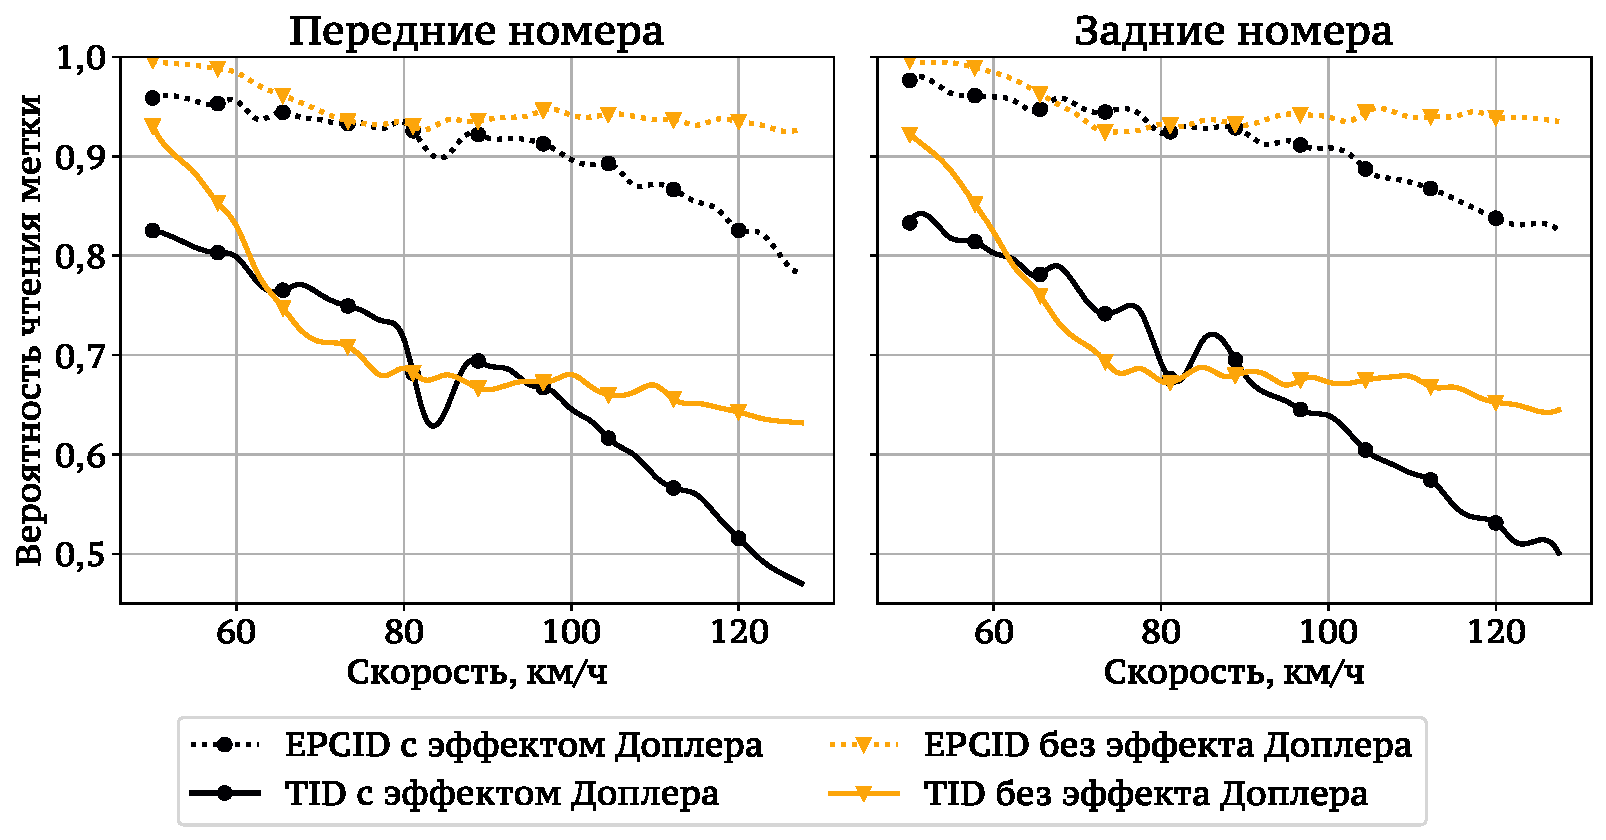
\includegraphics[width=0.9\textwidth]{chapter2/ch2_identification_doppler}
  }
	\caption{Влияние эффекта Доплера на вероятность успешного чтения метки при M = 4, Tari = 12,5~мкс}
	\label{fig:ch2_identification_doppler}
\end{figure}

Также было проведено численное исследование влияния эффекта Доплера, см. рис.~\ref{fig:ch2_identification_doppler}. Как видно из приведённых результатов, эффект Доплера оказывает существенное влияние на вероятность чтения меток, особенно при чтении TID на высоких скоростях "--- в этом случае эффект Доплера может снижать вероятность успешного чтения метки на 10--20~\%.

\begin{figure}[h]
	\centerfloat{
    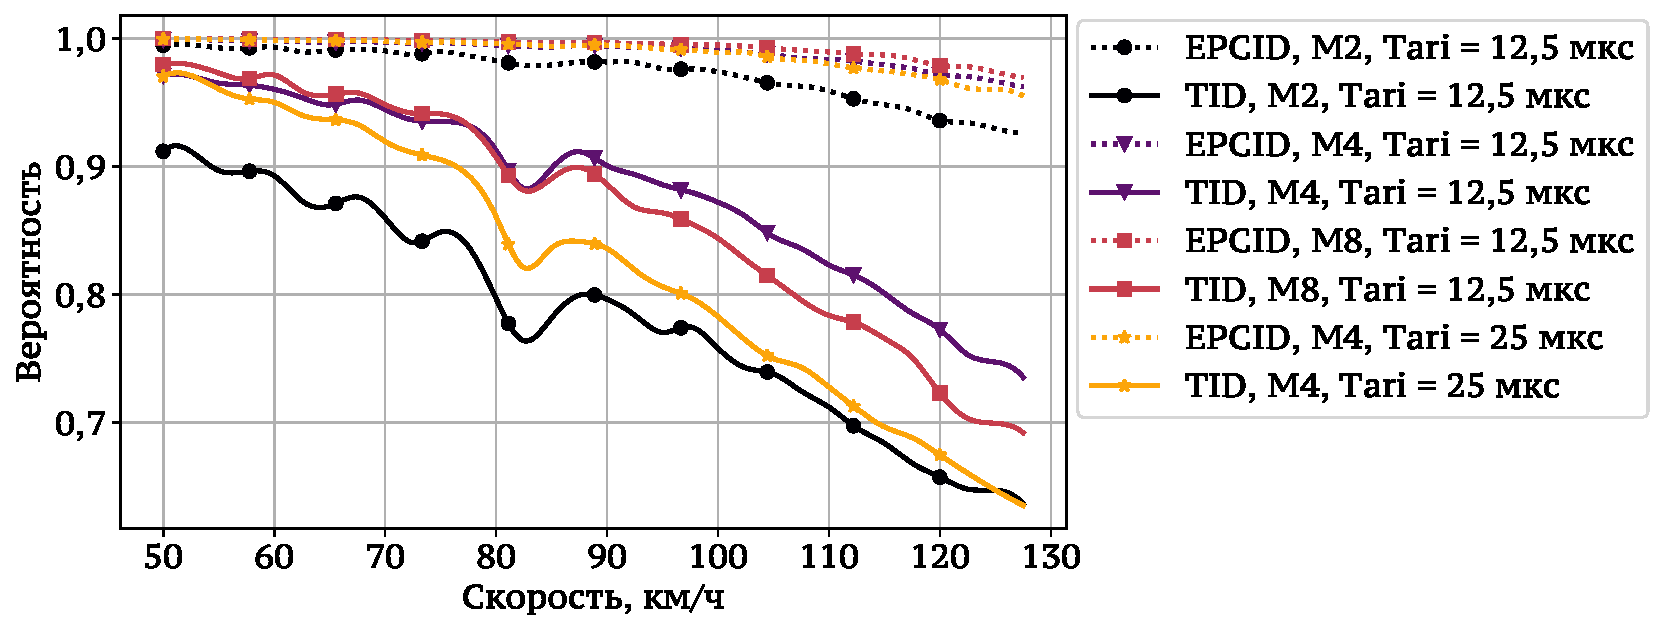
\includegraphics[width=0.9\textwidth]{chapter2/ch2_vehicle_identification_rate}
  }
	\caption{Вероятность идентификации автомобиля с метками на переднем и заднем номере, идентифицируемого по любой из меток}
	\label{fig:ch2_vehicle_identification_rate}
\end{figure}

Результаты расчета вероятности идентификации автомобилей показаны на рис.~\ref{fig:ch2_vehicle_identification_rate}. При проведении расчётов считалось, что автомобиль может быть идентифицирован по любой метке, т.е. для успешной идентификации было достаточно единожды прочитать метку в переднем или заднем номере. Полученные результаты сопадают с данными, полученных в ходе эксперимента в городе Казань (см. главу 5), в котором использовалось значение M=4 и Tari = 12,5~мкс, а вероятность идентификации составила около 92--95\%, в зависимости от точки идентификации, при идентификации меток по EPCID и TID. Из приведенных результатов видно, что эти значения дают наилучшую вероятность идентификации быстро движущихся автомобилей. Также можно видеть, что значения M = 8 и Tari = 25~мкс дают хорошие результаты на небольшой скорости, но затем сильно деградируют и на высоких скоростях дают вероятность, близкую к случаю использования гораздо менее надежных параметров M = 2 и Tari = 12,5~мкс. Как отмечалось ранее, это связано с тем, что при высоких скоростях длительность раунда становится слишком большой и у метки остаётся мало шансов передать свои идентификаторы.



%%%%%%%%%%%%%%%%%%%%%%%%%%%%%%%%%%%%%%%%%%%%%%%%%%%%%%%%%%%%%%%%%%%%%%%%%%%%%%%%
\section{Заключение}\label{sec:ch2_conclusion}
%%%%%%%%%%%%%%%%%%%%%%%%%%%%%%%%%%%%%%%%%%%%%%%%%%%%%%%%%%%%%%%%%%%%%%%%%%%%%%%%
В главе были представлены следующие результаты.
\begin{enumerate}
	\item Рассмотрены основные особенности системы радиочастотной идентификации автомобилей. На основе анализа протокола радиочастотной идентификации EPC Gen2 выделены факторы, влияющие на её производительность.
	\item Предложена имитационная модель, учитывающая различные сценарии идентификации автомобилей (идентификация только по значению EPCID или по паре EPCID и TID), параметры протокола EPC Gen2 (длительности символов в командах считывателя, способы кодирования ответов меток, выбор сессий и значений их флагов, число слотов в раунде), настройки считывателя (периодичность смены антенн и отключения питания), а также особенности распространения сигналов (многолучевое распростренение, зависимость коэффициента отражения от материала дорожного покрытия, эффект Доплера).
	\item С помощью имитационной модели были получены зависимости вероятности идентификации как отдельных номеров, так и автомобилей, от скорости движения, а также от выбранных настроек протокола EPC Gen2.
\end{enumerate}

\FloatBarrier
           % Глава 2
% \chapter{Аналитическая модель системы радиочастотной идентификации автомобилей}\label{ch:ch3}


В предыдущей главе с помощью имитационной модели были получены результаты, показывающие, что периодическая смена значений флага инвентаризации сессии и переключение питания между антеннами приводят к увеличению количества раундов, в которых метка принимает участие (см. рис. \todo{Номер рисунка}{?}). Чтобы объяснить причину этого эффекта нужно учесть, что, согласно сделанным ранее допущениям, в случае обнаружения ошибки в передаче идентификатора меткой считыватель не передает ни повторные команды ACK, ни команды NACK, а переходит сразу к следующему слоту или раунду. Поэтому метка, не имея возможности узнать о произошедшей ошибке, инвертирует хранимое значение инвентаризационного флага текущей сессии (например, если флаг опроса в текущем раунде был равен $A$, то метка инвертирует флаг $A \rightarrow B$). Метка принимает участие в следующем раунде в одном из двух случаев: если считыватель сменил значение флага опроса (в нашем примере с $A$ на $B$), или если считыватель продолжает опрос со значением флага $A$, но перед этим сбросил питание на достаточно продолжительное время. В последнем случае не имеет значения, просто ли считыватель выключил передатчик, или же переключился на другую антенну -- лишь бы метка была выключена достаточно долго.

Имитационная модель, описанная ранее в предыдущей главе -- очень сложная, требующая значительного времени для получения статистически устойчивых результатов. Поэтому для более детального изчения этого эффекта была разработана аналитическая модель, основанная на неоднородных марковских случайных процессах. С помощью этой модели можно описать произвольный сценарий сбросов питания и переключения значений флагов сессий, учесть законы движения меток и оценить вероятность идентификации.

Аналитическая модель строится при ряде допущений. Для их четкого определения приводится описание модельного считывателя и меток, а после этого -- формальная постановка задачи, учитывающая введенные ограничения. Для описания работы считывателя вводится понятие сценария. Далее приводится описание раунда инвентаризации, вводятся формулы для оценки длительности раунда. Кроме того, приводится распределение вероятностей случайной величины, описывающей число меток, успешно передающих RN16 без коллизий. Далее опишем модель как пару случайных процессов, переходные вероятности которых зависят от сценария, позволяющих найти оценки длительностей отдельных раундов, и рассчитать вероятность идентификации метки. После этого приводятся выражения для расчета переходных вероятностей процессов, зависящих от заданого сценария. В конце приведем численные результаты и сделаем выводы.

Результаты, представленные в главе, были опубликованы в сборнике трудов конференции IEEE RFID'2018, индексируемом в Scopus и WoS \cite{RFID_IEEERFID2018}, а также представлены в трудах ВСПУ XIII \cite{RFID_VSPU2019}. Кроме того, доклады по полученным результатам были представлены на международных конференциях DCCN'2019 (Москва) и ICAAP\&SP'2019 (Коттайам, Индия).



% \section{Обзор литературы}
Протокол, лежащий в основе канального уровня стандарта EPC Gen-2 \cite{StdGen2}, "--- Framed Slotted ALOHA. Исходный протокол ALOHA был представлен в работе \cite{Abramson1970}. В этой же работе, на основе предположения о пуассоновском потоке передаваемых пакетов, была получена оценка пиковой пропускной способности сети как $1/(2e) \approx 0,186$. Позднее в работе \cite{Roberts1975} был описан способ повышения пропускной способности в два раза за счет разбиения времени на слоты (Slotted ALOHA).

Значительное число работ посвящено анализу производительности систем радиочастотной идентификации. Авторы пользуются эмпирическими методами \cite{Buettner2008}, используют аппарат марковских случайных процессов как с идеальным каналом \cite{Vogt2002, Wang2009, Vahedi2012, Vales-Alonso2009, Vales-Alonso2011, Tong2007, Vales-Alonso2017}, так и с каналом с ошибками \cite{DiMarco2014}, а также используют иные аналитические подходы для анализа производительности \cite{Ahmed2016, Yan2014, Jeon2009, Kim2007}. В ряде работ также сравнивается производительность протокола Frame Slotted ALOHA с альтернативными протоколами и расширениями \cite{Vahedi2014, LaPorta2011}.

Отметим работу \cite{Vales-Alonso2017}, в которой с помощью дискретной цепи Маркова исследуется эффект потери метками питания. Авторы описывают систему в виде двумерной цепи, моделируя изменение числа меток, которые продолжают участвоват в опросе, и число меток, уже передавших свои данные. В результате проведенного анализа, авторы находят оценки вероятности идентификации к концу раунда опроса и пропускную способность системы. В отличие от представленной в главе модели, потери пакетов возникают только вследствие коллизий, не учитываются сессии, и моделирование производится по слотами в одном раунде, а не по раундам. Также стоит выделить работу \cite{Pawowicz2020}, в которой идентификация транспорта с помощью UHF RFID рассматривается в контексте создания <<умных городов>>, и предлагается очень простая модель для оценки вероятности потери метки, то есть ее проезда области чтения без идентификации. Авторы делят область чтения на секции и, полагая, что секции имеют фиксированную длину, а передавшие свой идентификактор метки не участвуют в последующих раундах, предлагают простой метод расчета. Кроме того, в работе представлены результаты сравнения аналитических результатов и данных, полученных из стендового моделирования. Стоит отметить, что, как и в диссертационном исследовании, авторы \cite{Pawowicz2020} рассматривают изменения системы между раундами, в том числе "--- поступления и выходы метки из области чтения. В то же время, степень детализации модели в диссертационном исследовании существенно выше, используются более тонкие допущения.

Предложенная автором модель имеет ряд отличий. Во-первых, переходы марковской цепи происходят на границах раундов, а не слотов, и учитывают сбросы питания и смены флагов опроса меток. Во-вторых, модель учитывает потери произвольных пакетов из-за ненулевой битовой ошибки. В-третьих, модель состоит из двух марковский процессов, первый из которых нужен для расчета числа меток, участвующих в раундах, а второй "--- для оценки вероятности идентификации. В-четвертых, матрицы переходных вероятностей строятся в виде произведения матриц отдельных операций (проведение опроса, инвертирование флага опроса, сброс питания, добавление или удаление метки из области чтения). Из-за этого, с одной стороны, марковские процессы оказываются неоднородными и тяжелее в анализе, но, с другой стороны, делает предложенный метод очень гибким, и позволяет в дальнейшем расширить его на более сложные операции.





%%%%%%%%%%%%%%%%%%%%%%%%%%%%%%%%%%%%%%%%%%%%%%%%%%%%%%%%%%%%%%%%%%%%%%%%%%%%%%%%
\section{Ограничения и допущения}\label{sec:ch3_assumptions}
%%%%%%%%%%%%%%%%%%%%%%%%%%%%%%%%%%%%%%%%%%%%%%%%%%%%%%%%%%%%%%%%%%%%%%%%%%%%%%%%
Для построения аналитической модели введём ряд необходимых допущений и ограничений на считыватель и метки, а также опишем приближенный способ расчета распределения длительностей раундов.


%%% --------------------------------------------
\subsection{Модельный считыватель}
%%% --------------------------------------------
В определении \textbf{модельного считывателя} мы накладываем ограничения на область чтения, битовые ошибки в принятых ответах меток, длительности команд, схему раунда инвентаризации. Наиболее существенные ограничения касаются области чтения и битовых ошибок.

Будем считать, что метки движутся по прямой. \textbf{Областью чтения} модельного считывателя будем считать фиксированный интервал, в каждой точке которого метка имеет достаточно энергии для включения и приема команд от считывателя. Вне области чтения метки не работают, с единственным исключением: если метка, покидающая область чтения, уже принимает участие в раунде инвентаризации, считается, что она сможет передать свои ответы в любом из слотов.

Если при передаче ответа от метки произошла коллизия с ответом другой метки, считыватель не может принять ни один из ответов. Если же при передаче ответа коллизии не произошло, вероятность \textbf{битовой ошибки (BER)} в принятом ответе постоянна\footnote{Это наиболее существенное ограничение, которое позволяет игнорировать точное расположение меток в области чтения, а также изменчивость канала во времени из-за эффекта Доплера.} и равна $\beta$. Возникновение ошибок в каждом бите будем полагать независимым, т.е. вероятность успешного приёма $b$ бит от одной или нескольких меток есть $b^{1 - \beta}$.

Модельный считыватель не изменяет значения параметров Q, Tari, M, TRext, а также калибровочных интвервалов TRcal и RTcal. Число Q задает двоичный логарифм числа слотов, то есть число слотов $N_s = 2^Q$. Значение Tari "--- это длительность символа data-0, равная 6,25, 12,5, 18,75 или 25,0~мкс. Значение M задает способ кодирования ответов меток, оно принимает значение 0 для кодирования FM0 и 1, 2, или 3 для кодов Миллера длиной 2, 4 или 8 символов соответственно. TRext "--- это флаг, задание которого означает, что метка должна использовать расширенную преамбулу перед своими ответами. Наконец, калибровочные интервалы TRcal и RTcal нужны для корректного разделения нулей и единиц, и для вычисления меткой скорости передачи ответов. Также считыватель всегда использует одну и ту же сессию для опроса меток; для определенности и простоты будем считать, что считыватель всегда использует сессию S0.

\textbf{Длительности команд} будем считать фиксированными, игнорируя вариации, связанные с использованием кодировки PIE и полями, неизвестными заранее, "--- например, случайным числом RN16 в команде ACK или значением контрольных сумм. Длительности команд будем обозначать как $T\{\text{msg}\}$, где $\text{msg}$ -- название команды. Интервалы\footnote{Диапазоны интервалов $T_1, T_2 \text{ и } T_3$ определены в табл. 6.16 стандарта EPC Gen.2. В тексте используются стандартные обозначения этих интервалов; в тех случаях, когда смысл $T_i$ может быть неверно истолкован, будет приведено дополнительное пояснение.} времени между концом команды и началом ответа метки ($T_1$), между концом ответа метки и началом следующей команды ($T_2$), а также между последовательными командами, если ответа от метки не было ($T_1 + T_3$), считаются постоянными.

Считыватель не использует команды Select, NACK, QueryAdjust, а также повторные команды ACK. Для чтения банков памяти используется только команда Read, передаваемая после получения ответа на команду Req\_RN. Команда Read всегда направлена на один и тот же банк памяти и запрашивает чтение одного и того же числа слов.

В каждый момент модельный считыватель может выполнять одну из \textbf{трех операций}: производить опрос меток в раунде инвентаризации, сбрасывать питание или изменять флаг опроса. Операции выполняются последовательно, ненулевую длительность имеют только операции инвентаризации и сброса питания.

\begin{enumerate}
	\item \textbf{Операция сброса питания} занимает время $T_\Delta$, на это время считыватель отключает питание. Отключение и последующее включение питания происходят мгновенно. После включения считыватель готов сразу начать инвентаризацию с флагом Target, равным A.

	\item \textbf{Операция смены флага инвентаризации} осуществляется мгновенно, в результате её выполнения инвертируется флаг сессии, по которому производится опрос меток (поле Target команды Query).

	\item \textbf{Операция инвентаризации} заключается в выполнении раунда опроса меток, начинается с передачи команды Query и завершается вместе с последним тактом.
\end{enumerate}

При оценке длительности раундов инвентаризации будем считать время распространения сигналов константой, равной $\delta$.


%%% --------------------------------------------
\subsection{Модельные метки}
%%% --------------------------------------------
Будем считать, что любой \textbf{модельной метке} всегда достаточно энергии в области чтения для включения и успешного приёма команд считывателя без ошибок. Также предполагаем, что метка при включении всегда сбрасывает значение хранимого флага в $A$, то есть длительность хранения флага всегда меньше, чем время отключения считывателя. Модельные метки не учитывают содержимое полей PC и слов XPC\_W1 и XPC\_W2 при формировании ответов на команды ACK. Для определенности будем предполагать, что в этих ответах метки передают PC, EPC и CRC. Длину EPCID считаем одинаковой для всех меток.

\textbf{Длительности ответов меток} будем считать известными и фиксированными. Будем обозначать их так же, как и длительности команд: $T_\text{msg}$, где $\text{msg}$ "--- название ответа. Размеры ответов в битах будем обозначать как $|\text{msg}|_b$.

Также будем считать, что метки не используют паролей, считывателю не нужно передавать команду Access при чтении банков памяти. Команда Kill не рассматривается, и метка не может быть в <<убитом>> состоянии, когда при включении она сразу попадает в состояние KILLED и не отвечает на любые команды.




%%%%%%%%%%%%%%%%%%%%%%%%%%%%%%%%%%%%%%%%%%%%%%%%%%%%%%%%%%%%%%%%%%%%%%%%%%%%%%%%
\section{Постановка задачи}\label{sec:ch3_problem_definition}
%%%%%%%%%%%%%%%%%%%%%%%%%%%%%%%%%%%%%%%%%%%%%%%%%%%%%%%%%%%%%%%%%%%%%%%%%%%%%%%%
Будем считать, что метки движутся по одной прямой, а область чтения, в которой метки получают достаточно энергии для работы, является интервалом $(0, L)$. Пусть функция $x(t)$ определяет закон движения меток так, что $x(0) = 0,\; \exists\,T_L: x(T_L) = L$ и $\forall\, t \in (0, T_L): x(t) \in (0, L)$, а $\forall t > T_L: x(t) > L$. Метки появляются в известные моменты времени $a_1, a_2, a_3, \dots$ в точке $x=0$, их движение определяется функциями $x_i(t) \equiv x(t - a_i)$. Другими словами, метки движутся одинаково со сдвигом по времени, могут ускоряться, замедляться или моментально изменять свое местоположение, но после первого покидания области чтения, которое обязательно должно произойти, более никогда не возвращаются в неё.

Так как законы движения меток $x_i(t)$ известны и детерминированы, число меток в области чтения в момент $t$ можно определить как функцию $N(t) = |\{ i:\: a_i \leqslant t \leqslant a_i + T_L \}|$. Для корректного определения случайных процессов потребуем, чтобы эта функция была ограничена сверху, то есть $\exists \overline{N} = \max\limits_{t \geqslant 0} N(t)$. Для этого достаточно потребовать, чтобы существовал интервал $\Delta t$, такой, что $\forall i: a_{i+1} - a_i \geqslant \Delta t$.

Благодаря допущению о постоянстве BER при приеме ответов от меток, в дальнейшем будет гораздо проще построить модель, так как единственной существенной величиной, характеризующей множество меток, будет функция $N(t)$, а не отдельные значения координат $x_i(t)$ или скоростей $x'_i(t)$ меток. Хотя это допущение является очень сильным, оно может быть более или менее существенно в зависимости от взаимного положения меток и считывателя. Например, при движении меток по горизонтали на конвейерной ленте и горизонтальном размещении антенны считывателя над лентой уровень сигнала будет более равномерным, чем при размещении меток на машинах, а считывателя "--- под углом к дороге.

Последнее допущение относительно области чтения заключается в том, что метки покидают область чтения только на границе раундов. Другими словами, если в раунде приняло участие $n$ меток, то любая метка остается в области чтения до конца и может ответить считывателю в любом из слотов.

Пусть $r \in \mathbb{N}$ -- произвольный номер раунда инвентаризации. Поведение считывателя характеризуется значением опрашиваемого флага $X_r \in \{A,B\}$ и признаком сброса питания после раунда $e_r \in \{0,1\}$.

\begin{defn}
	\textit{Спецификацией раунда} будем называть пару значений опрашиваемого флага и признака сброса питания $(X, e)$, которую будем сокращенно обозначать символом $\alpha \defeq X^{e}$.
\end{defn}

Например, $\alpha_5 = B^{1}$ означает, что в пятом раунде считыватель ведет опрос по флагу инвентаризации $B$ и после раунда сбрасывает питание, а $\alpha_2 = A^{0}$ говорит о том, что во втором раунде опрос идет по флагу $A$ и питание в конце не сбрасывается.

\begin{defn}\label{def:ch3_reader_scenario}
	\textit{Сценарием работы считывателя} $\bm{\alpha} = \alpha_1 \alpha_2 \dots \alpha_R$ будем называть последовательность спецификаций раундов конечной длины $R$.
\end{defn}

Будем считать, что после $R$-го раунда считыватель начинает <<проигрывать>> сценарий с самого начала, с первого раунда. Например, переключение флага каждые два раунда со сбросом питания на каждом четвертом можно описать как сценарий $A^0, A^0, B^0, B^1$.

Под \textit{идентификацией метки} мы будем понимать, как и в ранее во второй главе, либо успешную передачу EPCID метки, либо передачу TID.


\begin{probl}\label{problem:ch3_id_prob}
	Пусть известны законы движения меток $x_i(t) \equiv x(t - t_i)$, вероятность битовой ошибки в передаче ответов $\beta$ и сценарий работы считывателя $\bm{\alpha} = \alpha_1 \alpha_2 \dots \alpha_R$, а также размеры и длительности команд считывателя и ответов меток. Пусть также для идентификации меток требуется только EPCID (или комбинация EPCID и TID). Требуется найти вероятность, с которой каждая метка будет успешно идентифицирована.
\end{probl}

Для решения этой задачи опишем два случайных процесса: \textit{фоновый процесс}, моделирующий число меток, участвующих в каждом раунде, и \textit{основной процесс}, моделирующий проезд области чтения отдельно взятой меткой и позволяющий оценить вероятность её идентификации. Для описания переходов основного процесса необходимо иметь оценку длительностей раундов, которую можно вычислить, исходя из оценки числа участвующих в каждом раунде меток. Последнюю оценку получим с помощью итерационного расчета стационарного распределения фонового процесса.


%%%%%%%%%%%%%%%%%%%%%%%%%%%%%%%%%%%%%%%%%%%%%%%%%%%%%%%%%%%%%%%%%%%%%%%%%%%%%%%%
\section{Моделирование раундов инвентаризации}\label{sec:ch3_inventory}
%%%%%%%%%%%%%%%%%%%%%%%%%%%%%%%%%%%%%%%%%%%%%%%%%%%%%%%%%%%%%%%%%%%%%%%%%%%%%%%%
Прежде, чем перейти к построению пространства состояний и операций над ним, рассмотрим подробнее процесс идентификации меток и найдем оценки следующих величин:

\begin{itemize}
	\item вероятность $P_n(m)$ передачи EPCID $m$ метками из $n$;
	\item вероятность $p_\text{id}$ успешной идентификации отдельной метки;
	\item средняя ожидаемая длительность $\tau = \tau(n)$ раунда с $n$ метками;
	\item максимальная длительность раунда $\tau_{max}$.
\end{itemize}

\begin{figure}[htb]
	\centerfloat{
		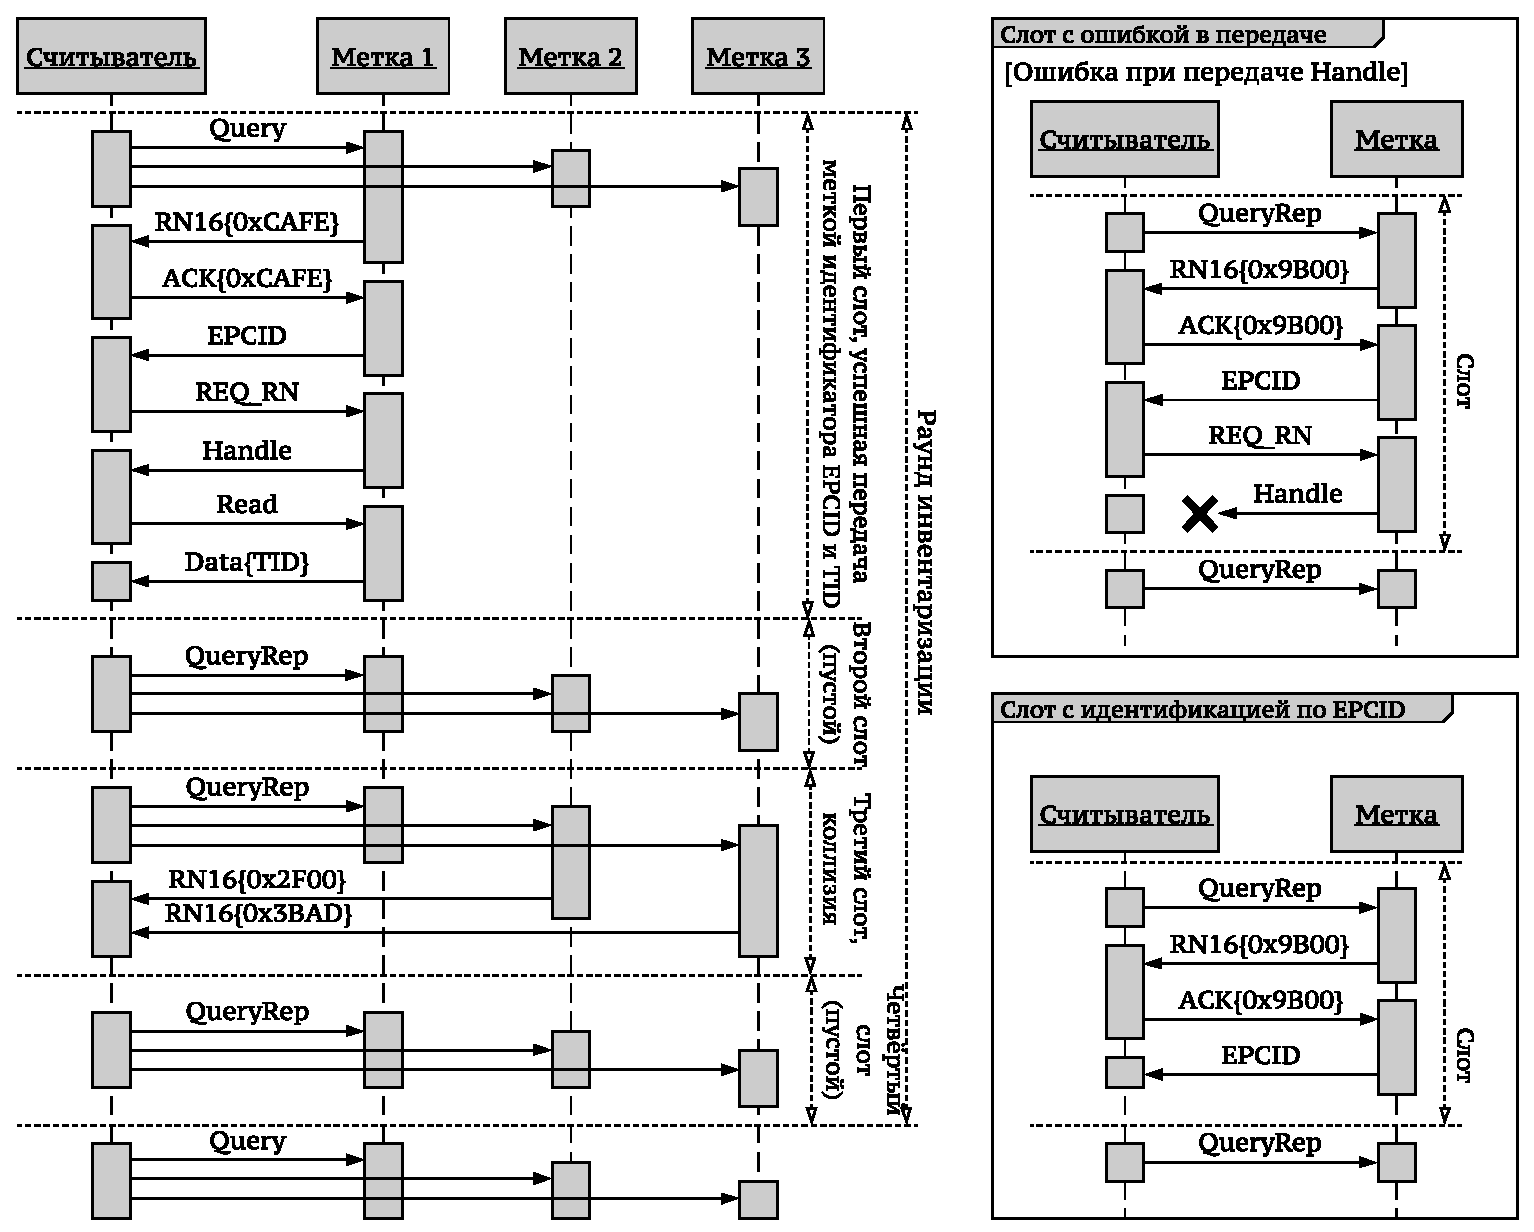
\includegraphics[width=1.0\textwidth]{chapter3/ch3_inventory_round}
  }
  \legend{Справа вверху "--- пример слота, в котором произошла ошибка в передаче ответа Handle. Справа внизу "--- пример слота, в котором метка успешно передает идентификатор, если идентификация происходит только по EPCID.}
  \caption[Пример раунда опроса при идентификации по EPCID и TID.]{Пример раунда инвентаризации с $Q=2$ и числом слотов $N_s=2^Q=4$ в случае идентификации метки по EPCID и TID. }
  \label{fig:ch3_inventory_round}
\end{figure}

Пример раунда инвентаризации показан на рис.~\ref{fig:ch3_inventory_round}. В этом примере предполагается, что параметр $Q = 2$, то есть число слотов $N_s = 2^Q = 4$, и в раунде участвует три метки. Первая метка выбрала для передачи первый слот, а вторая и третья -- третий. Идентификация метки происходит по комбинации EPCID и TID, поэтому в первом слоте считыватель после получения EPCID запрашивает случайное слово RN16 командой Req\_RN и использует его для контроля доставки в команде Read. В ответ на последнюю метка передает содержимое своего банка памяти TID. Если бы идентификация происходила только по EPCID, то первый слот был бы проще, обмен сообщениями выглядел бы как на правом нижнем фрагменте. Справа вверху показан пример слота, в котором произошла ошибка в передаче одного из ответов. Так как модельный считыватель не передает команды повторно, слот на этом завершается, метка остается неидентифицированной.

Ошибка может произойти при передаче любого из ответов. Учитывая то, что BER постоянен и равен $\beta$, вероятность успешной передачи ответа $\text{msg}$ можно найти как:

\begin{equation}\label{eq:ch3_response_err}
	P_\text{rx}\{\text{msg}\} = (1 - \beta)^{|\text{msg}|},
\end{equation}
где $|\text{msg}|$ -- длина ответа $\text{msg}$ в битах.

В дальнейшем потребуется оценивать число меток, участвующих в очередном раунде. Введём следующее определение.

\begin{defn}
	Назовем метку \textit{активной}, если она находится в области чтения, и ее значение флага сессии совпадает с передаваемым считывателем в поле Target команды Query. Значение этого поля будем называть \textit{флагом опроса}.
\end{defn}
\begin{rem}
	Следует подчеркнуть, что все модельные метки являются пассивными в техническом смысле слова, то есть они работают только в поле действия считывателя и не содержат автономного источника питания. Данное определение активности "--- исключительно логическое. Оно было выбрано, так как наиболее точно и лаконично описывает состояние метки.
\end{rem}

Обозначим $\mu_0$ "--- число пустых слотов в раунде, $\mu_1$ "--- число слотов с ответом единственной метки без коллизий и $\mu_2$ "--- число слотов с коллизиями. Для дальнейших расчетов нам потребуются распределения вероятностей случайных величин $\mu_0$ и $\mu_1$. Распределение $\mu_0$ определяется следующим образом:

\begin{equation}\label{eq:ch3_empty_slots}
	\mathbb{P}\{\mu_0 = z\} = \frac{1}{N_s^n} C_{N_s}^z {n\brace N_s-z} (N_s - z)!,
\end{equation}
где ${ n\brace N_s-z }$ "--- число Стирлинга 2-го рода, то есть число способов разбиения $n$ меток по $N_s - z$ непустым подмножествам.

Вероятность события $\{ \mu_1 = m \}$, то есть того, что ровно $m$ меток выбрали уникальные слоты и ответят считывателю без коллизий, будем обозначать как $\overline{P}_n(m) = \mathbb{P}\{ \mu_1 = m \}$, и будем вычислять с помощью формулы, приведенной в работе \cite{Vales-Alonso2011}:

\begin{equation}\label{eq:ch3_nocol_pnm}
	\overline{P}_n(m) = \mathbb{P}\{ \mu_1 = m \} = \frac{N_s! n!}{m! N_s^n} \sum\limits_{z=0}^{n-m}
		\frac{(-1)^z (N_s - m - z)^{(n - m - z)}}{(n - m - z)! z! (N_s - m - z)!}
\end{equation}

Сделаем два замечания относительно формул \eqref{eq:ch3_empty_slots} и \eqref{eq:ch3_nocol_pnm}. Во-первых, в \eqref{eq:ch3_nocol_pnm} предполагается, что число активных меток $n$ не превосходит числа слотов $N_s$. Во-вторых, на практике обе формулы неудобно применять из-за очень больших чисел в числителях и знаменателях уже при $N_s > 8$, то есть $Q = \log_2 N_s > 3$. Частично эту проблему удается решить группировкой множителей, но не во всех случаях, поэтому при численных расчетах для вычисления обеих вероятностей будем пользоваться методом Монте-Карло.

\begin{prop}\label{prop:ch3_pnm}
	Если в раунде инвентаризации участвует $n > 0$ меток, $P_\text{rx}\{\text{RN16}\}$ -- вероятность успешной передачи ответа RN16, а $\overline{P}_n(k)$ -- вероятность того, что ровно $k \leqslant n$ меток выбрали такие слоты, которые не выбрали другие метки, то вероятность того, что ровно $m \leqslant n$ меток изменят после раунда хранимое значение флага определяется следующим выражением:
	\begin{equation}\label{eq:ch3_pnm}
		P_n(m) = \sum\limits_{i=m}^{n}\overline{P}_n(i) C_i^mx \left(P_\text{rx}\{\text{RN16}\}\right)^m
			\left(1 - P_\text{rx}\{\text{RN16}\}\right)^{i - m},\; m \leqslant n
	\end{equation}
\end{prop}
\begin{proof}
	Метка передает идентификатор, если ей пришла команда ACK со случайным словом, совпадающим с переданным ранее меткой в ответе RN16. Согласно сделанным предположениям, это происходит, когда метка единственной передавала своё случайное слово RN16 в слоте, без коллизий с другими метками, и это слово было успешно доставлено\footnote{Если бы использовалась более точная модель интерференции, получение ответа было бы возможно также, например, если сигнал от другой меxтки был в том же слоте, но очень ослабленный.}. Тогда событие $X$:

	$$
	X = \text{<<ровно $m$ из $n$ меток передали идентификаторы>>}
	$$
	можно представить в виде суммы непересекающихся событий $X = \sum\limits_{i=m}^n Y_i$, где:
	$$
	\begin{aligned}
	Y_i = &\text{<<ровно $i$ из $n$ меток передали RN16 без коллизий,}\\
		  &\text{и ровно $m$ из $i$ из них было принято без ошибок>>}.
	\end{aligned}
	$$

	По формуле полной вероятности, учитывая независимость выбора слотов метками и возникновения ошибок в передаче их ответов, а также независимость возникновения ошибок в каждом переданном метками бите, получаем цепочку равенств, доказывающих утверждение:

	\begin{align*}
		P_n(m) &= \mathbb{P}\{X\} = \sum\limits_{i=m}^{n} \mathbb{P}\{Y_i\}\\
		&\begin{aligned}= \sum\limits_{i=m}^{n}(
			&\mathbb{P}\{\text{ровно $i$ из $n$ меток выбрали свободные слоты}\} \times\\
			& \mathbb{P}\{\text{ровно $m$ из $i$ меток успешно передали RN16}\})
			\end{aligned}\\
		&=\sum\limits_{i=m}^{n} \overline{P}_n(i) \times \left(C_i^m(P_\text{rx}\{\text{RN16}\})^m
			(1 - P_\text{rx}\{\text{RN16}\})^{i - m}\right)
	\end{align*}

\end{proof}

Для того, чтобы удостовериться, что $P_n(m)$ корректно описывает вероятность, докажем, что $\sum\limits_{m = 0}^n P_n(m) = \sum\limits_{i=0}^n \overline{P}_n(i) = 1$ (справедливость последнего равенства утверждается в работе \cite{Vales-Alonso2011}). Действительно,
$$
\begin{aligned}
	\sum\limits_{m=0}^n P_n(m) &=
		\sum\limits_{m=0}^n \sum\limits_{i=m}^n \overline{P}_n(i) C_i^m
			P_\text{rx}\{\text{RN16}\}^m (1 - P_\text{rx}\{\text{RN16}\})^{i-m}\\
	&= \sum\limits_{i=0}^n \sum\limits_{m=0}^i \overline{P}_n(i) C_i^m
			P_\text{rx}\{\text{RN16}\}^m (1 - P_\text{rx}\{\text{RN16}\})^{i-m}\\
	&= \sum\limits_{i=0}^n \overline{P}_n(i) \sum\limits_{m=0}^i C_i^m
			P_\text{rx}\{\text{RN16}\}^m (1 - P_\text{rx}\{\text{RN16}\})^{i-m}\\
	&= \sum\limits_{i=0}^n \overline{P}_n(i) \left( P_\text{rx}\{\text{RN16}\} + (1 - P_\text{rx}\{\text{RN16}\}) \right)^i\\
	&= \sum\limits_{i=0}^n \overline{P}_n(i)
\end{aligned}
$$

Вероятность успешной идентификации зависит от того, что используется в качестве идентификатора: EPCID или комбинация TID и EPCID. Условную вероятность успешной идентификации метки при условии отсутствия коллизии при её передаче будем обозначать как $p_{\text{id}}$:

\begin{equation}\label{eq:ch3_p_id}
	p_{\text{id}} = \begin{cases}
		P_{\text{rx}}\{\text{EPCID}\}, &\text{только EPCID}\\
		P_{\text{rx}}\{\text{EPCID}\}P_{\text{rx}}\{\text{Handle}\}P_{\text{rx}}\{\text{TID}\},&\text{EPCID и TID}
	\end{cases}
\end{equation}

Для вычисления оценки средней длительности раунда, воспользуемся приближенной схемой расчёта в допущении о независимости определения типов слотов. Будем считать, что каждый слот может иметь один из трёх типов: пустой слот (без ответа метки), слот с коллизией (ошибка при передаче RN16) и слот с ответом без коллизии. Обозначим через $t_0$ длительность пустого слота, $t_1^{\text{(epc)}}$ и $t_1^{\text{(tid)}}$  "--- средние длительности слотов с ответом без коллизий при идентификации по EPCID или по TID соответственно, а через $t_2$ "--- длительность слота с коллизией. Эти длительности могут быть вычислены следующим образом:

\begin{equation}\label{eq:ch3_slot_durations}
	\begin{aligned}
		t_0 =\;& T_\text{QRep} + T_1 + T_3\\
		t_1^{\text{(epc)}} =\;& T_\text{QRep} + (T_1 + T_2) +
			T_\text{RN16} + P_{rx}\{\text{RN16}\} \times \\
			&\left( T_\text{ACK} + (T_1 + T_2) + T_\text{EPCID} \right)\\
		t_1^{\text{(tid)}} =\;& T_\text{QRep} + (T_1 + T_2) +
				T_\text{RN16} + P_{rx}\{\text{RN16}\} \times \\
			&( T_\text{ACK} + (T_1 + T_2) + T_\text{EPCID} + P_{rx}\{\text{EPCID}\} \times \\
			&\quad (T_\text{Req\_RN} + (T_1 + T_2) + T_\text{Handle} 	+ P_{rx}\{\text{Handle}\} \times \\
			&\quad\quad(T_\text{Read} +(T_1 + T_2) + T_\text{TID})))\\
		t_1 =\;& \begin{cases}
			t_1^{\text{(epc)}}, &\text{только \text{EPCID}}\\
			t_1^{\text{(tid)}}, &\text{\text{EPCID} и \text{TID}}
 		\end{cases}\\
 		t_2 =\;& T_\text{QRep} + (T_1 + T_2) + T_\text{RN16}
	\end{aligned}
\end{equation}

Согласно допущению, вероятности слотов определяются независимо. Обозначим $p_0(n)$, $p_1(n)$ и $p_2(n)$ веротности того, что произвольный слот пуст, содержит ответ ровно одной метки или коллизию, соответственно. Эти вероятности можно вычислить, используя \eqref{eq:ch3_empty_slots} и \eqref{eq:ch3_nocol_pnm}:

\begin{equation}\label{eq:ch3_slot_probs}
	\begin{aligned}
		p_0(n) =\;& \frac{1}{N_s} \mathbb{E} \mu_0 = \frac{1}{N_s} \sum\limits_{i=0}^{N_s} i \mathbb{P}\{\mu_0 = i\}\\
		p_1(n) =\;& \frac{1}{N_s} \mathbb{E} \mu_1 = \frac{1}{N_s} \sum\limits_{i=0}^{N_s} i \mathbb{P}\{\mu_1 = i\}\\
		p_2(n) =\;& 1 - p_0(n) - p_1(n)
	\end{aligned}
\end{equation}

С помощью соотношений \eqref{eq:ch3_slot_durations} и \eqref{eq:ch3_slot_probs} длительность раунда $\tau(n)$ можно определить как сумму математического ожидания длительности слота и, если после раунда сбрасывается питание, длительности этого сброса:

\begin{equation}\label{eq:ch3_round_duration_of_n}
	\tau_r(n) = N_s \sum\limits_{i=0}^{2}p_i(n)t_i +
		(T_\text{Query} - T_\text{QRep}) +
		e_r T_\downarrow,
\end{equation}
где $n$ "--- число меток, участвующих в раунде, $e_r$ "--- индикатор сброса питания после опроса, а $T_\downarrow$ "--- длительность сброса. Слагаемое $(T_\text{Query} - T_\text{QRep})$ необходимо, так как при расчете длин слотов $t_i$ предполагалось, что каждый слот начинается с команды QRep, хотя первый слот начинается с более длинной команды Query.

Хотя в действительности распределение величин $\mu_0$, $\mu_1$ и $\mu_2$ не являются независимыми, приведенный способ расчета очень простой и позволяет получить достаточно точную оценку длительности раундов. Так, на рис.~\ref{fig:ch3_round_durations_validation} показан расчет с помощью описанной аналитической модели и метода Монте-Карло при различных значениях BER и числе участвующих в опросе меток от 0 до 20 (остальные параметры были фиксированы, число слотов $N_s = 2^Q = 16$). Можно видеть, что допущение о независимости определения типа слота оказывает минимальное влияние на точность оценки.

\begin{figure}[htb]
	\centerfloat{
		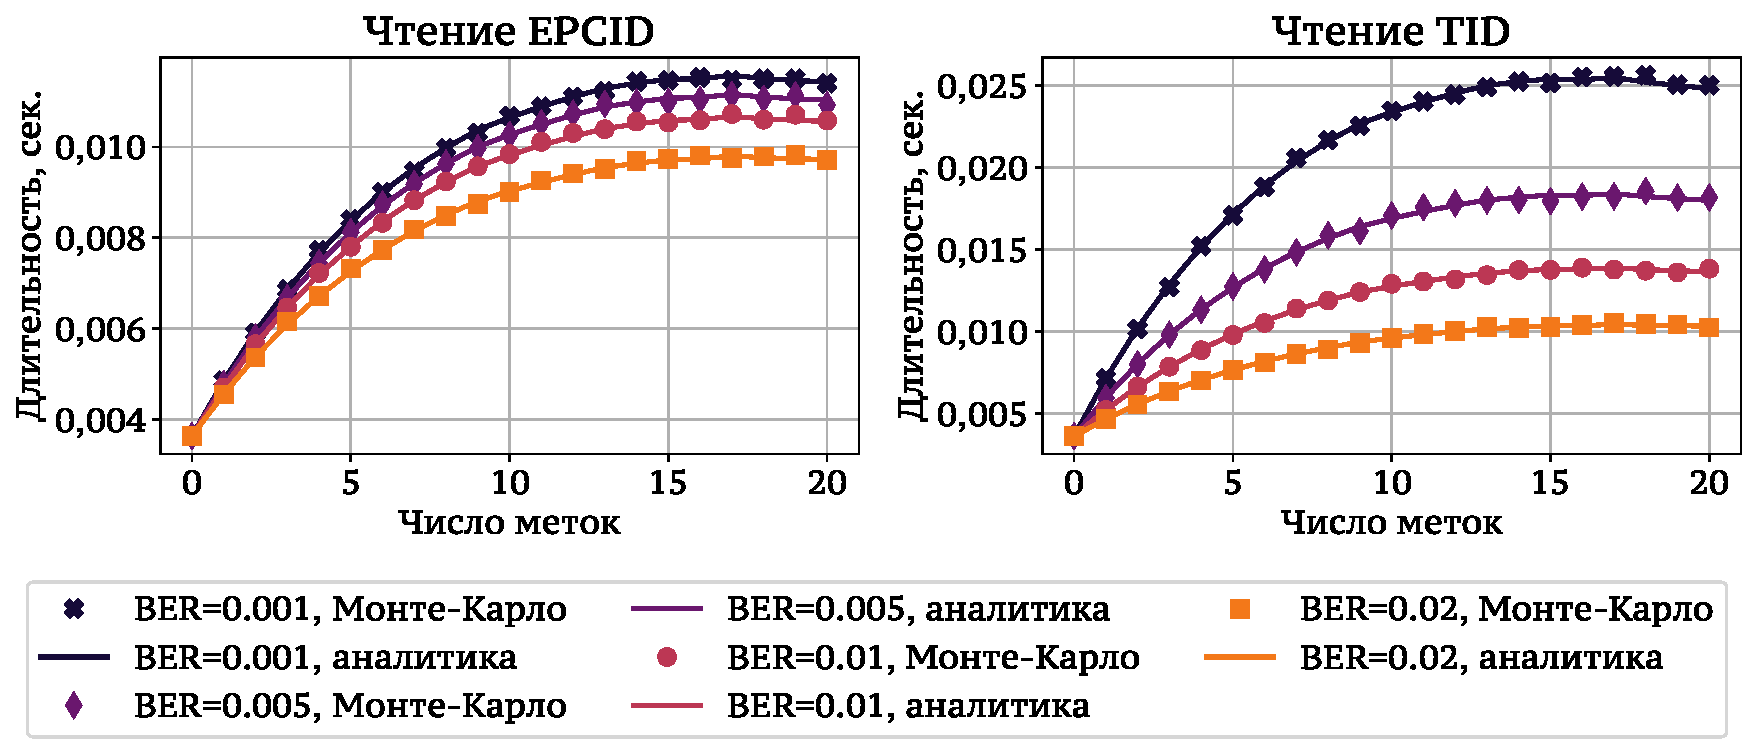
\includegraphics[width=1.0\textwidth]{chapter3/ch3_round_durations_validation.pdf}
  }
  \caption[Валидация модели расчета средрней длительности раундов.]{Сравнение результатов расчета средней длительности раундов с помощью аналитической модели и метода Монте-Карло.}
  \label{fig:ch3_round_durations_validation}
\end{figure}


Если известно распределение вероятностей числа меток, участвующих в раунде, $\bm{\pi} \in \mathbb{R}^{\overline{N}+1}$, где $\pi_i$ "--- вероятность того, что в системе ровно $i$ активных меток, $i \in [0, \overline{N}]$, то среднюю длину раунда можно опередлить как математическое ожидание $\tau_r = \mathbb{E} \tau_r(n)$:

\begin{equation}\label{eq:ch3_round_duration_avg}
	\tau_r = \sum\limits_{i=0}^{\overline{N}} \pi_i \tau_r(i)
\end{equation}

Пользуясь выражениями для длительностей слотов $t_1, t_2$ и $t_3$, можно найти оценку максимальной длительности раунда $\tau_{max}$:

\begin{equation}\label{eq:ch3_max_round_duration}
	\tau_{max} = \begin{cases}
 		\overline{N} t_1 + (N_s - \overline{N}) t_0, &\overline{N} \leqslant N_s\\
 		(N_s - 1) t_1 + t_2, &\overline{N} > N_s.
 	\end{cases}
\end{equation}
Справедливость этого выражения следует из того, что $t_0 < t_2 < t_1$ (значение $T_3$ заведомо не превышает $T_\text{RN16}$): если слотов больше, чем меток, то максимум достигается, когда все метки успешно передают свои идентификаторы. Если же слотов меньше, то в самом длинном раунде все слоты кроме одного будут содержать успешные передачи, а в одном слоте произвойдет коллизия оставшихся $\overline{N} - (N_s - 1)$ меток.



%%%%%%%%%%%%%%%%%%%%%%%%%%%%%%%%%%%%%%%%%%%%%%%%%%%%%%%%%%%%%%%%%%%%%%%%%%%%%%%%
\section{Вычисление оценки длительностей раундов}\label{sec:ch3_round_durations}
%%%%%%%%%%%%%%%%%%%%%%%%%%%%%%%%%%%%%%%%%%%%%%%%%%%%%%%%%%%%%%%%%%%%%%%%%%%%%%%%

%%% --------------------------------------------
\subsection{Размеченные сценарии и элементарные операции}
%%% --------------------------------------------
Пусть в некоторый момент времени в системе находится $N$ меток, $0 \leqslant N \leqslant \overline{N}$, и пусть $n$ из них активны, то есть готовы принять участие в раунде, в котором опрос просходит по флагу $X \in \{A, B\}$, $0 \leqslant n \leqslant N$.

Число $n$ может измениться по трем причинам (см. рис.~\ref{fig:ch3_operations}). Во-первых, если флаг опроса $X$ после очередного раунда инвентаризации не изменяется, и $n' \leqslant n$ меток в этом раунде передали свои EPCID, то эти метки инвертировали свои флаги и в следующем раунде не будут принимать участие, то есть активными будут $n - n'$ меток. Если же после раунда считыватель инвертирует флаг опроса $X$, то число активных меток будет $N - (n - n')$. Во-вторых, само число $N$ может измениться, если какая-либо метка покинула систему, или, наоборот, вошла в нее. Это изменение может затронуть число активных меток $n$, если систему покинула активная метка (в этом случае $n$ уменьшается на единицу), или если метка поступила в систему, и текущий флаг опроса равен $A$ (значение $n$ увеличивается на единицу). Наконец, в-третьих, считыватель может сбросить питание, после чего все метки будут хранить значение флага, равное $A$. Если считыватель продолжит опрос с флагом $X = A$, то активными будут все $n = N$ меток, а если с флагом $B$, то активных меток точно не будет, $n = 0$.

\begin{figure}[htb]
	\centerfloat{
    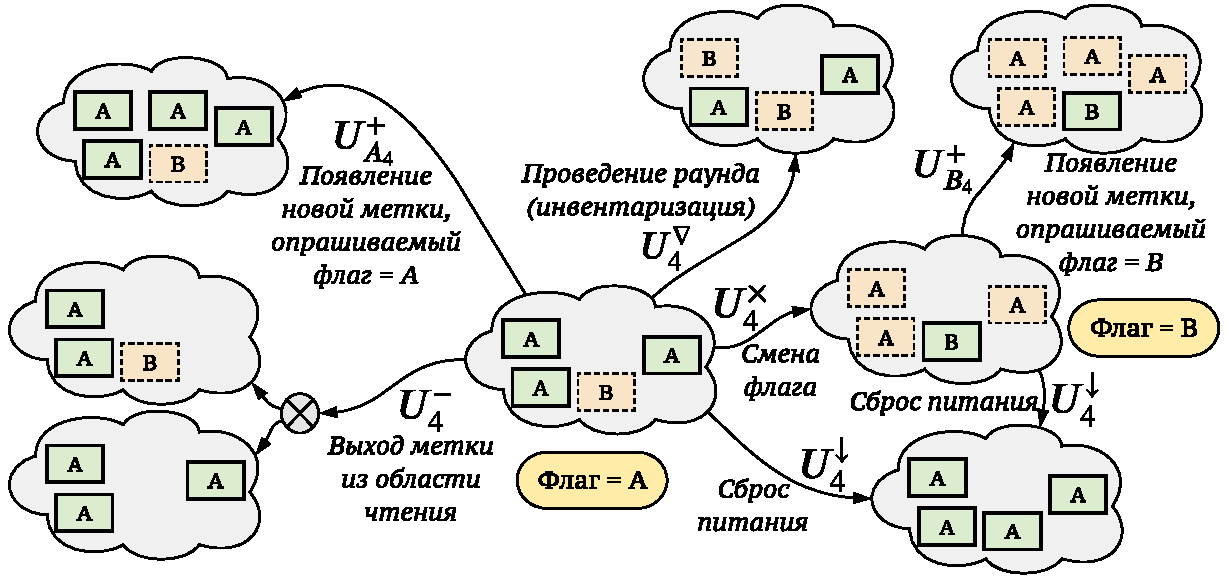
\includegraphics[width=1.0\textwidth]{chapter3/ch3_operations}
  }
  \caption{Операции над системой.}
  \label{fig:ch3_operations}
\end{figure}

Таким образом, изменение числа активных меток происходит в результате пяти действий, которые в дальнейшем будем называть \textit{элементарными операциями}: проведения раунда инвентаризации ($U_N^\nabla$), изменения флага опроса ($U_N^\times$), сброса питания ($U_N^\downarrow$), добавления метки в систему ($U_N^+$) или выхода метки ($U_N^-$). Как будет показано далее, с помощью композиции элементарных операций можно описать, как изменяется распределение числа активных меток после каждого раунда. Однако первый вопрос "--- как по известному сценарию работы считывателя определить, какие элементарные операции нужно выполнять.

В начале главы было введено понятие сценария (см. определение~\ref{def:ch3_reader_scenario}) как последовательности $\bm{\alpha} = \alpha_1 \alpha_2 \dots \alpha_R$, где $\alpha_r = (X_r, e_r) \equiv X_r^{e_r}$ "--- спецификация раунда. По заданному сценарию можно описать операцию, которую считыватель должен провести над метками. Например, если $\bm{\alpha} = \alpha_1 \alpha_2 \alpha_3 \alpha_4 = A^0 B^1 A^0 A^1$, то в первом раунде нужно провести опрос ($U_N^\nabla$) и инвертировать флаг опроса с $A$ на $B$ ($U_N^\times$), во втором раунде "--- провести опрос и сбросить питание ($U_N^\downarrow$), в третьем раунде просто провести опрос, а в четвертом "--- провести опрос и сбросить питание.

В сценарии содержится только информация о работе считывателя, однако нет данных о том, когда метки появляются и выходят из системы. Обозначим число меток в области чтения в $r$-м раунде как $N_r$, а число меток, покидающих и поступающих в область чтения за время $r$-го раунда как, соответственно, $\Delta_r^-$ и $\Delta_r^+$.  Предположим, что удалось установить, сколько меток было в области чтения в начале первого раунда $N_1$, а также все значения $\{\Delta_r^-\}_{r=1}^R$ и $\{\Delta_r^+\}_{r=1}^R$. Отметим, что для раунда $r > 1$ число меток можно вычислить как $N_r = N_{r-1} - \Delta_{r-1}^- + \Delta_{r-1}^+$.  Введем следующее определение, объединяющее сценарий $\bm{\alpha}$ и оценки $\{ N_r \}$, $\{ \Delta_r^- \}$ и $\{ \Delta_r^+ \}$.

\begin{defn}\label{ref:ch3_marked_scenario}
  Будем называть \textit{размеченным сценарием} последовательность символов $\widetilde{\bm{\alpha}} = \widetilde{\alpha}_1 \widetilde{\alpha}_2 \dots \widetilde{\alpha}_R$, каждый из которых имеет вид пятерки $\alpha_r = (X_r, e_r ; N_r, \Delta^-_r, \Delta^+_r)$. Символы $\alpha_r$ будем называть \textit{размеченными спецификациями раундов}. В дальнейшем будем использовать нотацию $[\prescript{N_r}{\Delta_r^-} X_{\Delta_r^+}^{e_r}]$, причем для сокращения записи иногда не будем указывать $\Delta_r^-$, $\Delta_r^+$ и $e_r$, если они равны нулю.
\end{defn}

Возвращаясь к предыдущему примеру, если сценарий $\bm{\alpha} = A^0 B^1 A^0 A^1$, $N_1 = 5$, $\{ \Delta_r^+ \} = \{ 0, 1, 0, 1 \}$ и $\{ \Delta_r^- \} = \{ 1, 0, 0, 1 \}$, то $\{ N_r \} = \{ 5, 4, 5, 5 \}$ и
$$
\begin{aligned}
	\widetilde{\bm{\alpha}} &= \left( (A, 0; 5, 1, 0),\,
	(B, 1; 4, 0, 1),\,
	(A, 0; 5, 0, 0),\,
	(A, 1; 5, 1, 1)\right) =\\
	&= [\prescript{5}{1} A^{0}_{0}] [\prescript{4}{0} B^{1}_{1}] [\prescript{5}{0} A^{0}_{0}] [\prescript{5}{1} A^{1}_{1}]
		= [\prescript{5}{1}A] [B^{1}_{1}] [\prescript{5}{}A] [\prescript{5}{1} A^{1}_{1}]
\end{aligned}
$$
Для такого размеченного сценария уже можно полностью описать все действия над системой: в первом раунде после опроса ($U_5^\nabla$) нужно инвертировать флаг ($U_5^\times$) и удалить метку ($U_{B,5}^+$), во втором раунде "--- провести опрос ($U_4^\nabla$), сбросить питание ($U_4^\downarrow$) и добавить одну метку ($U_{A,4}^+$), в третьем "--- только провести опрос ($U_5^\nabla$), а в четвертом "--- провести опрос ($U_5^\nabla$), сбросить питание ($U_3^\downarrow$), удалить одну метку ($U_5^-$) и затем добавить еще одну метку ($U_{A_4}^+$). Отметим, что пример последнего раунда показывает, почему недостаточно знать число меток в каждом раунде, а важно также знать, сколько меток поступает и покидает область чтения.

Для построения размеченного сценария нужно найти число меток перед первым раундом, а также определить, сколько меток поступает и покидает систему в каждом раунде. Пусть модельное время начинается в момент $T_0$. Обозначим последовательность моментов начала раундов опросов как $\{ t_r \}_{r=1}^\infty$. Тогда $\Delta_r^+ = |\{ a_i :\: t_r \leqslant a_i < t_{r+1} \}|$ и $\Delta_r^- = |\{ a_i:\: t_r \leqslant a_i + T_L < t_{r+1} \}|$, а $N_1 = N(T_0)$. Таким образом, для нахождения $\Delta_r^-$ и $\Delta_r^+$ нужно знать, когда начинается каждый раунд, а для этого нужно вычислить оценки длительностей каждого раунда $\{ \tau_r \}$. Длительности раундов опроса $\{ \tau_r \}$ вычисляются с помощью выражений \eqref{eq:ch3_round_duration_of_n} и \eqref{eq:ch3_round_duration_avg}, но для их использования нужно знать распределение вероятностей числа меток $n$, принимающих участие в каждом раунде.

Прежде, чем перейти к решению вопроса о нахождении оценок длительностей раундов, отметим, что значение $N_r$ можно вычислить, как $N_r = N(T_0 + \tau_1 + \tau_2 + \dots + \tau_{r-1}).$ Величина $T_0$ может быть произвольной, но желательно устанавливать ее достаточно большой, чтобы избежать погрешности из-за краевых эффектов.


%%% --------------------------------------------
\subsection{Матрицы элементарных операций}\label{subsec:ch3_bg_elem_op_matrices}
%%% --------------------------------------------
Как отмечалось ранее, число активных меток является случайной величиной, так как в общем случае вероятность того, что в течение раунда инвентаризации ровно $n - n'$ меток передадут свои идентификаторы, меньше единицы. Рассмотрим случайный процесс $\{ \eta_r \in [0, \overline{N}] \}_{r=1}^\infty$, моделирующий число активных меток в системе. Время в этом процессе дискретно и увеличивается на единицу после выполнения операции. В дальнейшем, в качестве такой операции будет выступать выполнение раунда и всех действий, определенных спецификацией. Однако, в этом разделе, прежде чем ввести определение операции, моделирующей весь раунд, для удобства будем считать, что $r$ меняется после каждой \textit{элементарной} операции.

Пусть $U$ "--- одна из элементарных операций, число активных меток перед ее выполнения равно $\eta_r = n$, а после "--- $\eta_{r+1} = n'$, $n,n' \in [0,\overline{N}]$. В силу сделанных ранее допущений, в частности "--- о постоянстве BER во всей области чтения, каждую элементарную операцию будем задавать распределением вероятностей $\mathbb{P}\{\eta_{r+1} = n' | \eta_r = n\}$. Переходные вероятности операции $U$ можно задать в виде матрицы порядка $\overline{N} + 1$. Для удобства будем считать, что нумерация строк и столбцов в матрицах $U$ и элементов вектора $\bm{\pi}$ начинается с нуля, чтобы номера строк и столбцов в точности соответствовали числу активных меток; тогда $\{ U \}_{ij} = \mathbb{P}\{ \eta_{r+1} = j\; |\; \eta_{r} = i \}$. Рассмотрим переходные матрицы каждой из элементарных операций (см. рис.~\ref{fig:ch3_bg_trans}).

\begin{figure}[htb]
	\centerfloat{
    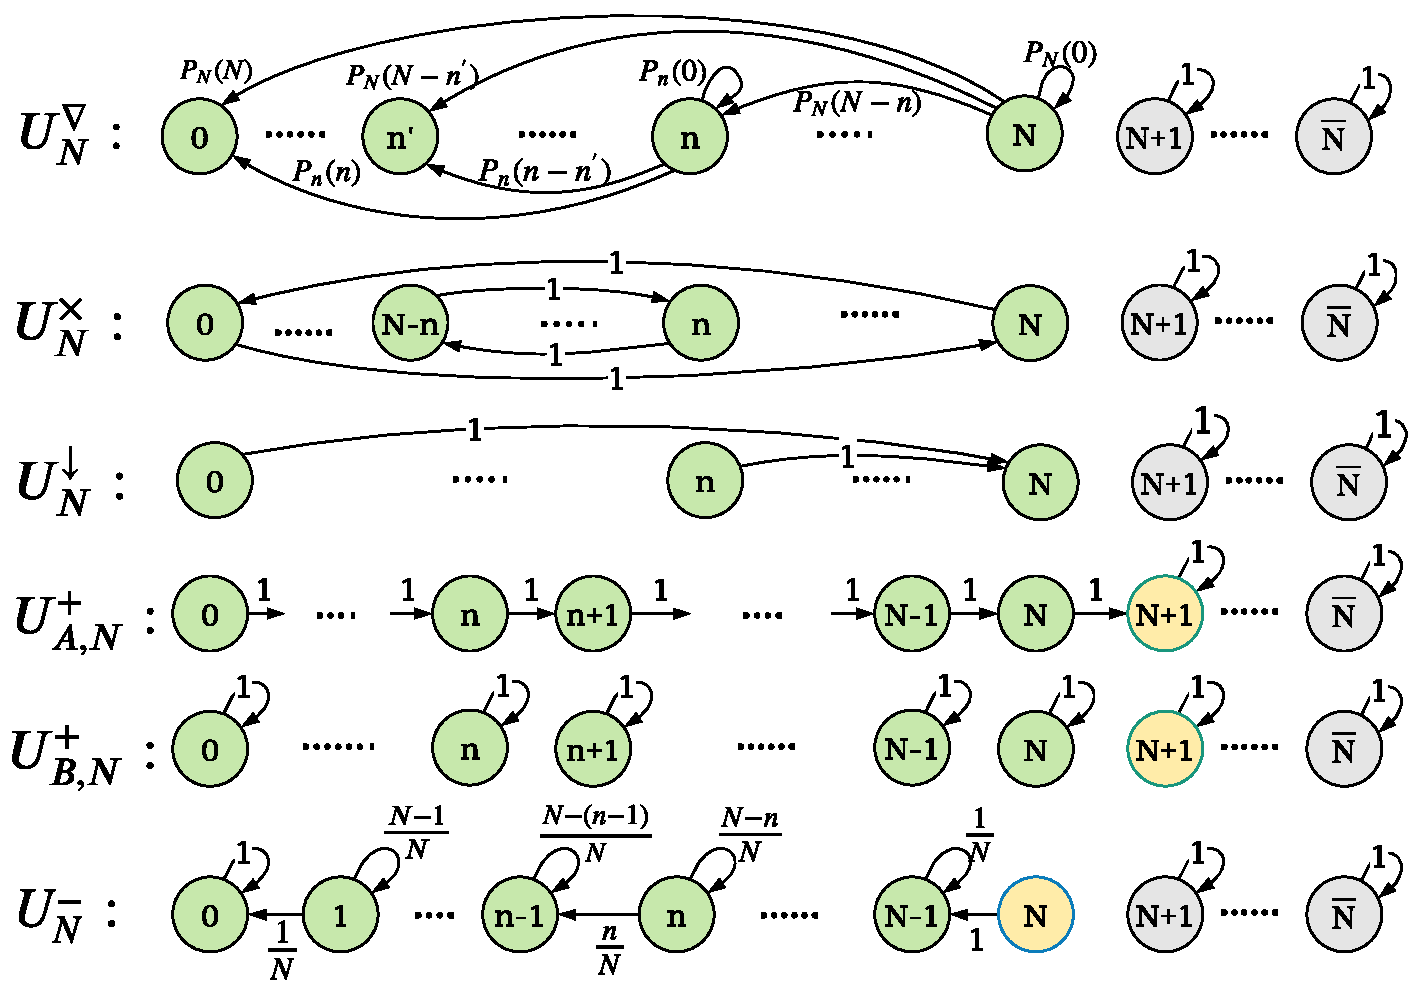
\includegraphics[width=0.9\textwidth]{chapter3/ch3_bg_trans}
  }
  \caption{Изменение числа активных меток при выполнении элементарных операций.}
  \label{fig:ch3_bg_trans}
\end{figure}

Применение операции опроса меток приводит к том, что часть меток передают (возможно, успешно) свои EPCID и инвертируют флаг. Непосредственно после этой операции флаг не меняется, питание не отключается, а метки не покидают и не поступают в область чтения. Вероятность того, что после опроса ровно $n'$ из $n$ меток будут активны, равна $P_n(n - n')$ (см. выражение~\eqref{eq:ch3_pnm}), а матрица $U_N^\nabla$ задается так:

\begin{equation}\label{eq:ch3_bg_inventory}
	\{ U_N^\nabla \}_{ij} = \begin{cases}
		P_i(i - j), & 0 \leqslant j \leqslant i \leqslant N\\
		1,          & N < i = j \leqslant \overline{N}\\
		0,          & \text{в остальных случаях.}
 	\end{cases}
\end{equation}

В результате инвертирования флага опроса неактивные метки становятся активными и наоборот, и число активных меток становится равным $N - n$:

\begin{equation}\label{eq:ch3_bg_switch}
	\{ U_N^\times \}_{ij} = \begin{cases}
 		1, & 0 \leqslant i \leqslant N,\; j = N - i\\
 		1, & N < i = j \leqslant \overline{N}\\
 		0, & \text{в остальных случаях.}
 	\end{cases}
\end{equation}

Сброс питания приводит к тому, что у всех меток в области чтения хранимое значение флага становится равным $A$. Так как после этого опрашивать метки по флагу $B$ не имеет практического смысла, будем считать, что флаг опроса также становится равным $A$, то есть все метки "--- активны:

\begin{equation}\label{eq:ch3_bg_power_off}
	\{ U_N^\downarrow \}_{ij} = \begin{cases}
 		1, & 0 \leqslant i \leqslant N,\; j = N\\
 		1, & N < i = j \leqslant \overline{N}\\
 		0, & \text{в остальных случаях.}
 	\end{cases}
\end{equation}

Выполнение операции добавления метки ведет к тому, что в системе становится на одну метку больше (то есть увеличивается $N$). Изменение числа активных меток зависит от текущего значения флага опроса: если флаг опроса $X = A$, то число активных меток увличивается, а если $X = B$, не изменяется:

\begin{equation}\label{eq:ch3_bg_tag_arrival}
	\begin{aligned}
		\{ U_{A,N}^+ \}_{ij} &= \begin{cases}
			1, & 0 \leqslant i < \overline{N}, \; j = i + 1\\
			1, & N+1 \leqslant i = j \leqslant \overline{N}\\
			0, & \text{в остальных случаях}
	 	\end{cases}\\
		U_{B,N}^+ &= I_{\overline{N}+1},
 	\end{aligned}
\end{equation}
где $I_{\overline{N}+1}$ "--- единичная матрица порядка $\overline{N}+1$.

Наконец, при выходе метки из области чтения число меток $N$ уменьшается. Изменение числа активных меток зависит от того, была ли покинувшая систему метка активной. Здесь необходимо сделать одно замечание. В идеале, нужно учитывать, какая метка находится ближе к области выхода, и смотреть, активна ли она. Однако, это привело бы к серьезному увеличению пространства состояний: вместо одного числа активных меток нужно было бы хранить в состоянии системы положения меток и значения их флагов. Поэтому при определении этой элементарной операции сделаем допущение о том, что покинуть систему может равновероятно любая метка. В этому случае вероятность изменения числа активных меток пропорциональна их числу в системе:

\begin{equation}\label{eq:ch3_bg_tag_departure}
	\{ U_{N}^- \}_{ij} = \begin{cases}
		\frac{i}{N},     & 0 < i \leqslant N,\; j = i - 1\\
		\frac{N - i}{N}, & 0 \leqslant i < N,\; i = j\\
		1,               & N \leqslant i = j \leqslant \overline{N}\\
		0,               & \text{в остальных случаях.}
 	\end{cases}
\end{equation}

Прежде, чем перейти к моделированию раундов инвентаризации, определенных размеченными сценариями, с помощью элементарных операций, сделаем замечание относительно элементов матриц. Можно видеть, что во всех матрицах справа внизу содержится единичный блок. Вообще говоря, строки при $i > N$ не имеют физического смысла: любая операция вида $U^\bullet_N$ применяется к системе, в которой находится $N$ меток. Было бы логично сделать так, чтобы все матрицы имели порядок $N+1$ ($N+2$ для $U_N^+$), то есть чтобы каждый элемент соответствовал возможному изменению числа активных меток, учитывая, что в системе перед выполнением операции находится ровно $N$ меток. Однако, далее потребуется рассматривать композиции элементарных операций, для чего их матрицы будут перемножаться. Можно видеть, однако, что вероятность попадания в состояние $n > N$ в результате выполнения любой из операций (за исключением $U_N^+$) равна нулю, и любое из состояний $n > N$ является поглощающим.




%%% --------------------------------------------
\subsection{Построение операций по размеченному сценарию}\label{subsec:ch3_bg_round_op_matrices}
%%% --------------------------------------------
Обозначим распределение вероятностей случайной величины $\eta_r$ как $\bm{\pi}^{(r)} \in \mathbb{R}^{\overline{N}+1}$. Здесь $\pi_n^{(r)} = \mathbb{P}\{\eta_r = n \}$ при $n \in [0, N_r]$, и $\pi_i^{(r)} \equiv 0$ при $i > N_r$. Если перед выполнением элементарной операции $U_i$ распределение вероятностей $\eta$ было $\bm{\pi}$, то распределение после ее выполнения будет $\bm{\pi}U_i$, после выполнения $U_{i+1}$ распределение будет $\bm{\pi} U_i U_{i+1}$ и так далее. Действительно, учитывая, что вероятность изменения $\eta_r$ вследствие выполнения операции определяется только текущим значением $\eta_r$ и типом элементарной операции, случайный процесс $\{ \eta_r \}$ будет неоднородным марковским процессом с дискретным временем, матрицы переходов которого есть матрицы операций.

\begin{figure}[htb]
	\centerfloat{
    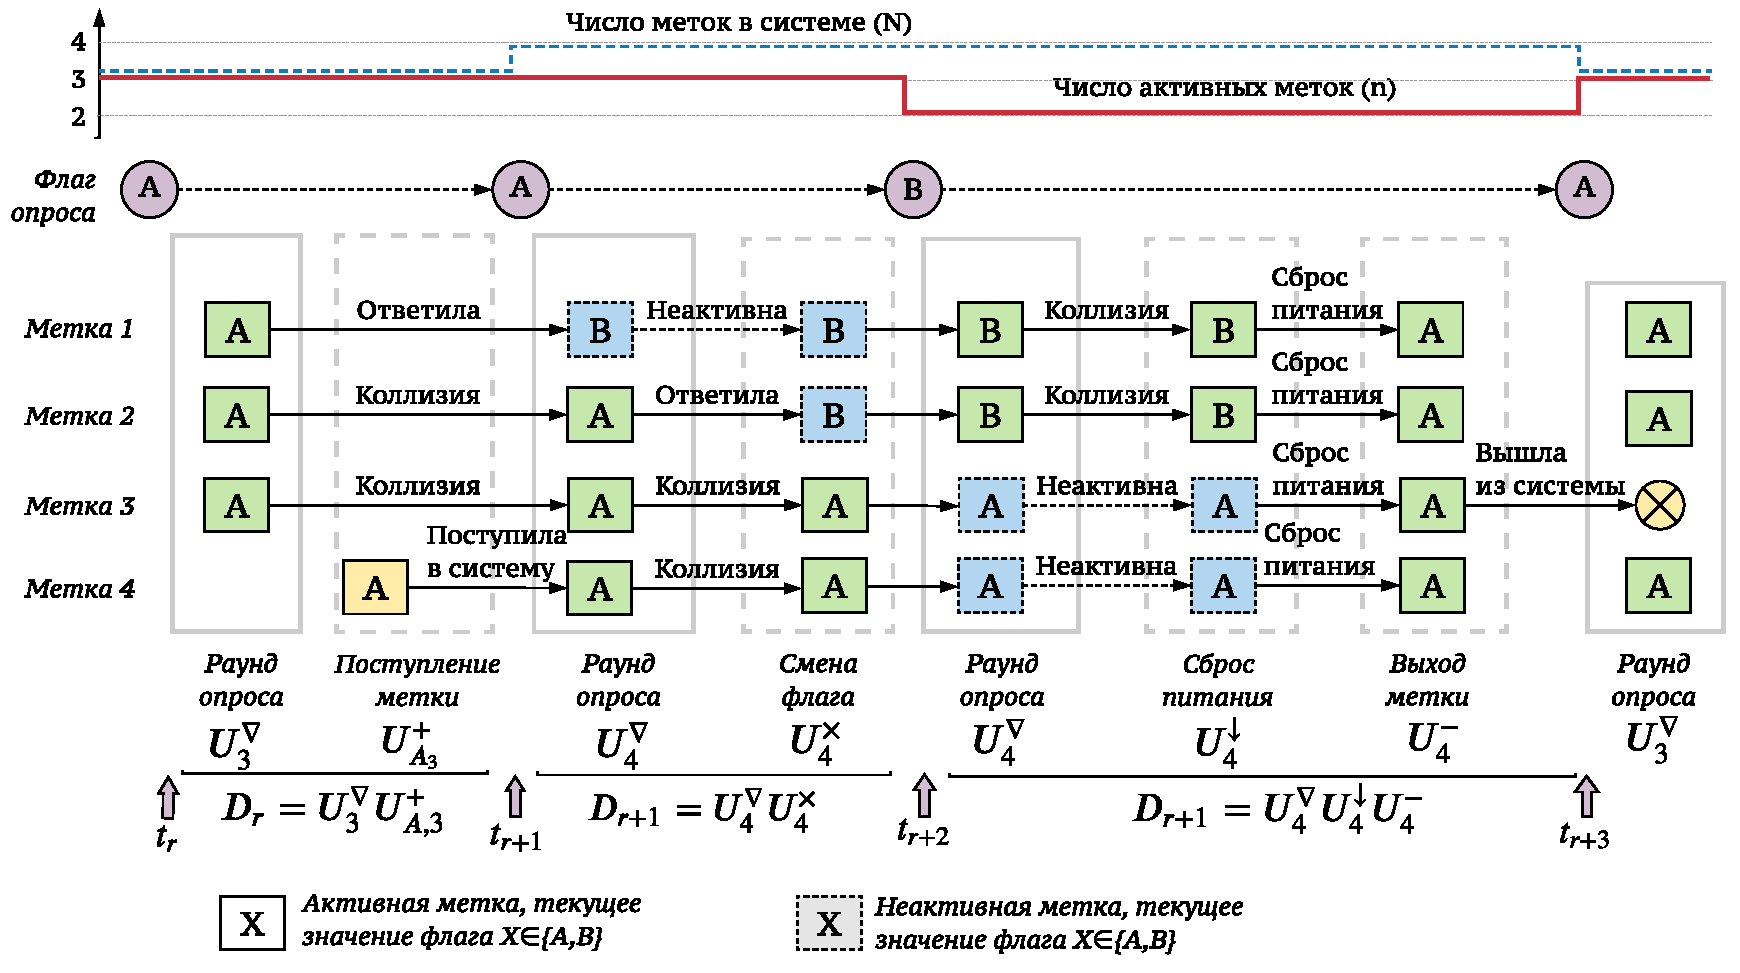
\includegraphics[width=1.0\textwidth]{chapter3/ch3_decomposition}
  }
  \caption{Пример представления раундов в виде операций, и декомпозиция этих операций до элементарных операций.}
  \label{fig:ch3_decomposition}
\end{figure}

Представим весь процесс изменения состояния системы в виде последовательности операций $D_r$, по одной операции на раунд опроса. Каждую операцию $D_r$ можно представить в виде композиции элементарных операций (см. пример~\ref{fig:ch3_decomposition}). Отсюда и далее будем полагать, что время в слуайном процессе $\eta_r$ (число активных меток) меняется на единицу в начале каждого раунда.

Рассмотрим расширенный размеченный сценарий $\widetilde{\bm{\alpha}} = \widetilde{\alpha}_1 \widetilde{\alpha}_2 \dots \widetilde{\alpha}_R$. Пусть $\widetilde{\alpha}_r = (X, N, e, \Delta^-, \Delta^+)$ и $\widetilde{\alpha}_{r+1} = (Y, \bullet, \bullet, \bullet, \bullet)$ (здесь $\bullet$ "--- произвольное значение). Все, что происходит с системой в $r$-м раунде, полностью описывается значениями текущего флага опроса $X$, числом меток $N$, количеством покидающих и поступающих в систему меток $\Delta^-$ и $\Delta^+$, признаком сброса питания после опроса $e$ и значением флага в следущем раунде $Y$.

\begin{figure}[htb]
	\centerfloat{
    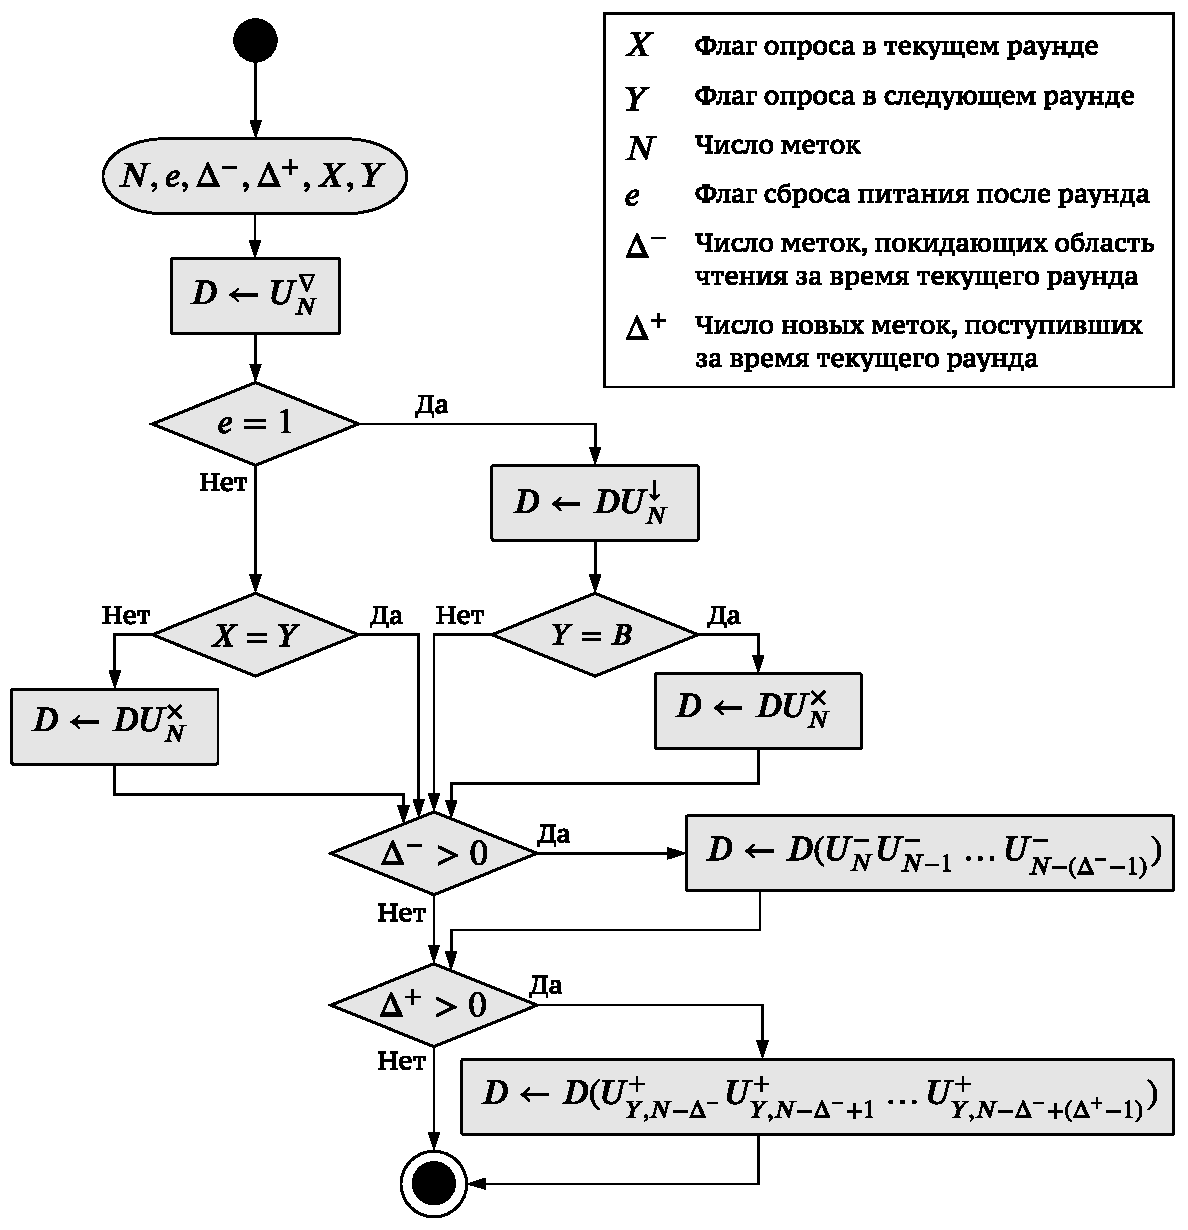
\includegraphics[width=0.8\textwidth]{chapter3/ch3_matrix_composition}
  }
  \caption{Алгоритм построения матрицы перехода $D$.}
  \label{fig:ch3_matrix_composition}
\end{figure}

Алгоритм построения матрицы $D = D_r$ приведен на рис.\ref{fig:ch3_matrix_composition}. Матрица $D$ представляется в виде произведения матриц элементарных операций $U_i$, причем первым множителем в этом произведении всегда является $U_N^\nabla$, то есть матрица операции инвентаризации меток. Далее, если считыватель выключается, то нужно умножить $D$ на $U^\downarrow_N$ и, если в следующем раунде считыватель опрашивает метки по флагу $Y = B$, умножить на матрицу операции смены флага $U^\times_N$. Если считыватель не выключается, то $D$ нужно умножить на матрицу $U^\times_N$ в том случае, если флаг опроса в следующем раунде инвертируется, то есть $X \neq Y$. Если за время опроса и отключения (если $e = 1$) счиытывателя одна или более меток покинули область чтения, то есть $\Delta^- > 0$, то умножаем $D$ на матрицы $U^-_N, U^-_{N-1}, \dots, U^-_{N-(\Delta^--1)}$ (так как после каждой операции вида $U^-_N$ число меток в области чтения становится меньше на единицу, уменьшается и нижний индекс). Если за время опроса в систему поступили метки, то есть $\Delta^+ > 0$, то аналогично умножаем матрицу $D$ на матрицы операций добавления меток $U^+_{Y,N'}, U^+_{Y,N'+1}, \dots, U^+_{Y,N+(\Delta^+-1)}$, где $N' = N - \Delta^-$.

Отметим, что порядок умножения матриц элементарных операций важен. К примеру, пусть в раунде $r+1$ считыватель ведет опрос по флагу $A$, и с ненулевой вероятностью все метки в конце раунда $r$ хранят флаг $B$, то есть число активных меток равно нулю ($\eta_r = 0$). Пусть также после раунда $r$ одна метка поступает в систему, а другая "--- покидает ее. Новая метка всегда хранит флаг сессии со значением $A$, то есть в данном случае будет активной в раунде $r+1$. Очевидно, что после этого в начале $(r+1)$-го раунда в системе обязательно будет хотя бы одна активная метка. Но если бы операция добавления учитывалась до операции удаления метки, то с вероятностью $1/{(N+1)}$ число активных меток уменьшилось бы до нуля. По тем же причинам, смена флага должна учитываться до добавления меток, но после сброса питания.

Вернемся к примеру расширенного сценария $\widetilde{\bm{\alpha}} = [\prescript{5}{1}A^{0}_{0}] [\prescript{4}{0} B^{1}_{1}] [\prescript{5}{0}A^{0}_{0}] [\prescript{5}{1}A^{1}_{1}]$. Для него представление в виде операций, моделирующих раунды, и декомпозиция до уровня элементарных операций, будет выглядеть так:

$$
\begin{aligned}
  \widetilde{\bm{\alpha}} =&
  [\prescript{5}{1}A^{0}_{0}] [\prescript{4}{0}B^{1}_{1}] [\prescript{5}{0}A^{0}_{0}] [\prescript{5}{1}A^{1}_{1}]
  	\Longrightarrow D_1\,, D_2\,, D_3\,, D_4, \text{ где}\\
  &\qquad D_1 = U^\nabla_5 U^\times_5 U^-_5\\
  &\qquad D_2 = U^\nabla_4 U^\downarrow_4 U^+_{A,4}\\
  &\qquad D_3 = U^\nabla_5\\
  &\qquad D_4 = U^\nabla_5 U^\downarrow_5 U^-_5 U^+_{A,4}
\end{aligned}
$$




%%% --------------------------------------------
\subsection{Расчет распределения числа активных меток}
%%% --------------------------------------------
Имея последовательность операций для размеченного сценария, можно рассчитать распределение вероятностей числа активных меток перед началом каждого раунда. Как отмечалось выше, случайный процесс "--- неоднородный марковский. Время в этом процесе увличивается на единицу на каждом раунде, а матрицами переходов являются $D_1, D_2, \dots D_R$. Так как после выполнения сценария ситема моделируется опять с начала  размеченного сценария, то после операции $D_R$ будут опять применяться операции $D_1, D_2, \dots D_R$. В общем случае можно записать это так:
$$
	D_r \equiv D_{(r - 1)\, (\textbf{mod } R) + 1}.
$$

Если процесс $\eta_r$ на $r$-м шаге имеет распределение $\bm{\pi}^{(r)}$, то после $r$-го раунда распределение будет $\bm{\pi}^{(r)} D_r$, после $r+1$ шага "--- $\bm{\pi}^{(r)} D_r D_{r+1}$ и так далее. Так как после $R$-й переходной матрицы опять используется $D_1$, то распределение процесса на $(r+R)$-м шаге будет
$$
	\bm{\pi}^{(r+R)} = \bm{\pi}^{(r)} D_r D_{r+1} \dots D_R D_1 \dots D_{r-1}.
$$
Обозначим произведение матриц, стоящих в правой части, как $\widetilde{D}_{r}$, то есть положим
$$
	\widetilde{D}_r = D_r D_{r+1} \dots D_R D_1 \dots D_{r-1}.
$$

Рассмотрим последовательность значений процесса $\{ \eta_r \}$ на шагах $r, r+R, r+2R, \dots$ и обозначим эту последовательность как $\{ \eta_i^{[r]} \}_{i=0}^\infty$, $\eta_i^{[r]} = \eta_{r+Ri}$. Так как процесс $\{ \eta_{i}^{[r]} \}$ является \hl{подпроцессом} марковского процесса $\{ \eta_r \}$, то он и сам является марковским, причем, в отличие от $\{ \eta_r \}$, он будет однородным: переходные матрицы между шагами задаются матрицей $\widetilde{D}_r$. Найти его стационарное распределение $\bm{\pi}^{(r)}$ можно из системы линейных уравнений:
$$
	\begin{cases}
		\bm{\pi}^{(r)} &= \bm{\pi}^{(r)} \widetilde{D}_r\\
		1 &= \sum\limits_{n=0}^{\overline{N}} \pi^{(r)}_n
	\end{cases}
$$
Из найденного вектора $\bm{\pi}^{(r)}$ можно найти $\bm{\pi}^{(r+1)} = \bm{\pi}^{(r)} D_r$, $\bm{\pi}^{(r+2)} = \bm{\pi}^{(r+1)} D_{r+1}$ и так далее. Таким образом, рассчитать распределение вероятностей перед каждым раундом $r = 1, 2, \dots, R$ можно, решив следующую систему уравнений:

\begin{equation}\label{eq:ch3_bg_pmf_system}
	\begin{cases}
		\bm{\pi}^{(1)} &= \bm{\pi}^{(1)} \widetilde{D}_1\\
		\bm{\pi}^{(2)} &= \bm{\pi}^{(1)} D_1\\
		\bm{\pi}^{(3)} &= \bm{\pi}^{(2)} D_2\\
		\dots&\\
		\bm{\pi}^{(R)} &= \bm{\pi}^{(R-1)} D_{R-1}\\
		1              &= \sum\limits_{n=0}^{\overline{N}} \pi^{(1)}_n
	\end{cases}
\end{equation}

Используя найденные распределения числа активных меток, с помощью формул \eqref{eq:ch3_round_duration_of_n} и~\eqref{eq:ch3_round_duration_avg} можно вычислить новые оценки длительностей раундов $\tau_r = \mathbb{E} \tau_r(n)$.



%%% --------------------------------------------
\subsection{Итерационный расчет оценок длительностей раундов}\label{subsec:ch3_iterative_algorithm}
%%% --------------------------------------------
В результате расчета $\tau_r$ по найденным распределениям $\{ \bm{\pi}^{(r)} \}_{r=1}^R$ оценки длительностей раундов могут измениться. Если изначально раунды предполагались сликом короткими или длинными, то после того, как будет найдено распределение числа активных меток, их длительности могут соответственно увеличиться или уменьшиться. Однако, так как моменты поступления меток $\{a_i\}$ и закон изменения числа меток $N(t)$ не зависят от длительностей раундов, то может измениться и размеченный сценарий.

Рассмотрим пример. Пусть задан сценарий $\bm{\alpha} = A^0 A^0 A^0 \dots$, в начальный момент в системе две метки и новая метка поступает на 120-й миллисекунде ($a_1 = 120$). Предположим изначально, что первые два раунда имеют длительность 100~миллисекунд (то есть $\tau_1 = \tau_2 = 100$). Тогда размеченный сценарий будет иметь вид $\widetilde{\alpha} = [\prescript{2}{}A] [\prescript{2}{}A_1] [\prescript{3}{}A] \dots$. Если после пересчета выяснится, что раунды имеют длительности $\tau_1 = 150$ и $\tau_2 = 95$, то новый размеченный сценарий будет иметь вид $\widetilde{\alpha}' = [\prescript{2}{}A_1] [\prescript{3}{}A_1] \dots$. Соответственно, изменятся и матрицы переходных вероятностей операций $D_r$, поэтому в итоге могут измениться и оценки $\{ \bm{\pi}^{(r)} \}$, и $\{ \tau_r \}$. Таким образом, может потребоваться многократный пересчет оценок $\tau_r$.

Итерационный алгоритм, позволяющий найти оценки длительностей раундов $\{ \tau_r \}$, принимает на вход сценарий $\bm{\alpha} = \alpha_1 \alpha_2 \dots \alpha_R$, закон изменения числа меток $N(t)$, максимально допустимую ошибку $\epsilon > 0$ и максимальное число итераций $\overline{K}$. Алгоритм выполняет следующие действия (см. рис.~\ref{fig:ch3_iterative_algorithm}).

\begin{figure}[htb]
	\centerfloat{
    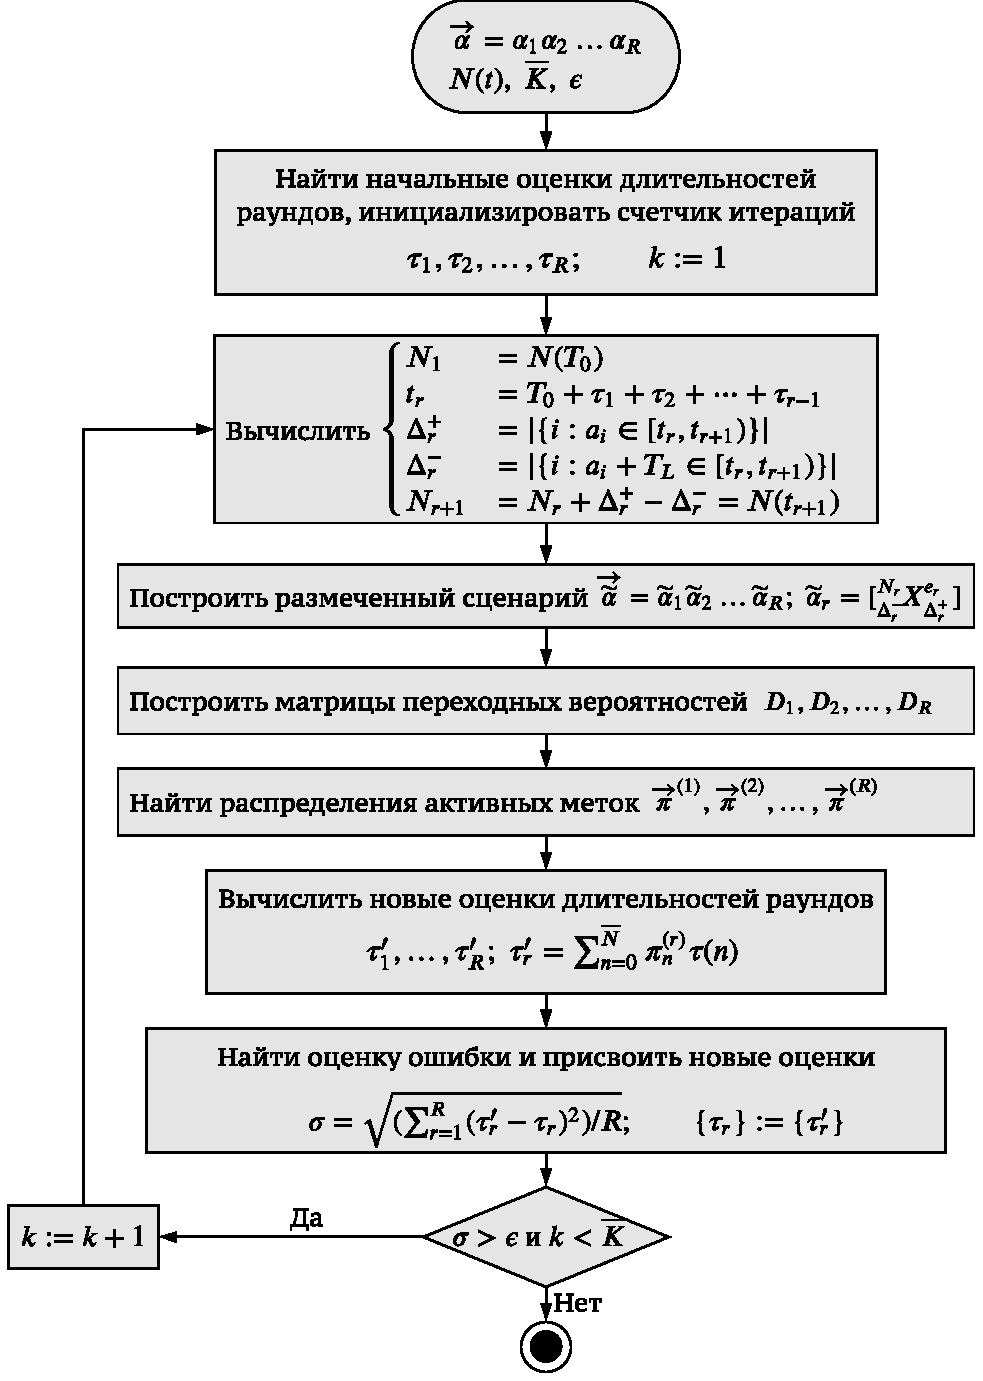
\includegraphics[width=0.7\textwidth]{chapter3/ch3_iterative_algorithm}
  }
  \caption{Итерационный алгоритм расчета длительностей раундов.}
  \label{fig:ch3_iterative_algorithm}
\end{figure}

\textit{Шаг 1}. Произвольно выбираются начальные оценки длительностей раундов $\tau_1, \tau_2, \dots, \tau_R$, а счетчик числа итераций $k$ выставляется равным единице.

\textit{Шаг 2}. Вычисляется число меток в системе в начале первого раунда $N_1$, время начало каждого раунда $t_r = T_0 + \tau_1 + \tau_2 + \cdots + \tau_{r-1}$, число поступивших и покинувших систему за $r$-й раунда меток $\Delta_r^+ = |\{i: t_r \leqslant a_i < t_{r+1}\}|$ и $\Delta_r^- = |\{i: t_r \leqslant a_i + T_L < t_{r+1} \}|$. Затем выичисляется число меток во втором и последующих раундах $N_r = N_{r-1} + \Delta_{r-1}^+ - \Delta_{r-1}^-$ (это же число можно получить как $N_r = N(t_r)$).

\textit{Шаг 3}. По найденным значениям $\{ N_r \}$, $\{ \Delta_r^+ \}$, $\{ \Delta_r^- \}$ и заданному сценарию $\bm{\alpha} = \alpha_1 \alpha_2 \dots \alpha_R$ строится размеченный сценарий $\widetilde{\bm{\alpha}} = \widetilde{\alpha}_1 \widetilde{\alpha}_2 \dots \widetilde{\alpha}_R$, $\widetilde{\alpha}_r = [\prescript{N_r}{\Delta_r^-} X^{e_r}_{\Delta_r^+}]$.

\textit{Шаг 4}. С помощью найденного размеченного сценария строятся матрицы переходных вероятностей $D_1, D_2, \dots, D_R$ процесса $\{ \eta_r \}_{r=1}^\infty$. Для нахождения матриц $D_r$ (см. блок-схему на рис.~\ref{fig:ch3_matrix_composition}) используются матрицы элементарных операций, которые задаются выражениями \eqref{eq:ch3_bg_inventory},~\eqref{eq:ch3_bg_switch},~\eqref{eq:ch3_bg_power_off},~\eqref{eq:ch3_bg_tag_arrival} и \eqref{eq:ch3_bg_tag_departure}.

\textit{Шаг 5}. Вычисляется стационарное распределение числа активных меток перед каждым раундом $\bm{\pi}^{(1)}, \bm{\pi}^{(2)}, \dots, \bm{\pi}^{(R)}$ как решение системы линейных алгебраических уравнений \eqref{eq:ch3_bg_pmf_system}.

\textit{Шаг 6}. С помощью найденных распределений вероятностей $\{ \bm{\pi}^{(r)} \}_{r=1}^R$ вычисляются новые оценки длительностей раундов $\tau'_1, \tau'_2, \dots, \tau'_R$, где $\tau'_r = \sum_{n=0}^{\overline{N}} \pi^{(r)}_n \tau(n)$, а длительность раунда для заданного числа активных меток $\tau(n)$ вычисляется с помощью \eqref{eq:ch3_round_duration_of_n}.

\textit{Шаг 7}. Вычисляется среднеквадратичное отклонение между предыдущей и новой оценкой длительностей раундов $\sigma = \sqrt{\sum_{r=1}^R (\tau'_r - \tau_r)^2 / R}$. Если $\sigma \leqslant \epsilon$ или число итераций $k$ достигло максимального $\overline{K}$, то последние вычисленные оценки $\{ \tau'_r \}_{r=1}^R$ возвращаются в качестве результата выполнения алгоритма, и он завершается. В противном случае, если $\sigma > \epsilon$ и $k < \overline{K}$, счетчик числа итераций $k$ увеличивается на единицу, найденные оценки $\{ \tau'_r \}$ используются вместо исходных $\{ \tau_r \}$, и алгоритм переходит на шаг 2.

Следует сделать несколько замечаний относительно работы алгоритма. Во-первых, в общем случае алгоритм может не сойтись к определенному набору значений $\{ \tau_r \}_{r=1}^R$ со сколь угодно малой точностью. Это связано с тем, что при нахождении оценок могут возникать эффекты, сходные с колебаниями: при одной оценке события изменения числа меток происходят в одних раундах, а при пересчете оценок "--- в других; но после еще одной или нескольких переоценки длительностей они опять начинают происходить в тех же раундах. Для того, чтобы алгоритм наверняка завершался приходится вводитб ограничение на число итераций. В то же время, в ходе интенсивных численных экспериментов алгоритм завершался всегда, причем в подавляющем большинстве случаев ему хватало всего двух итераций.

Во-вторых, в качестве входа стоит использовать не сам сценарий $\bm{\alpha} = \alpha_1 \alpha_2 \dots \alpha_R$, а его многократно увеличинную версию вида
$$
	\bm{\alpha}^{[L]} = \underbrace{\bm{\alpha} \dots\, \bm{\alpha}}_{L \text{ повторов}} =
		\underbrace{\alpha_1 \dots\, \alpha_R \; \alpha_1 \dots\, \alpha_R\; \dots \, \alpha_1 \dots\, \alpha_R}_{LR \text{ символов}}.
$$
Это приходится делать для того, чтобы в моделируемый участок времени попало достаточное число событий поступления и выхода меток из системы, так как обычно $a_{i+1} - a_i \gg \tau_{max}$. Чем больше $L$, тем точнее будут полученные результаты. Нужно, однако, учесть, что увеличение длины сценария ведет к увеличению времени расчета.

В-третьих, желательно начинать моделирование с того момента $T_0$, когда в системе уже находится некоторое количество меток. Так как переходная матрица $D_R$ строится по символам расширенного сценария $\widetilde{\alpha}_R = [\prescript{N_R}{\Delta_R^-} X^{e_R}_{\Delta_R^+}]$ и $\widetilde{\alpha}_1 = [\prescript{N_1}{\Delta_1^-} Y^{e_1}_{\Delta_1^+}]$, то если начинать моделирования с момента $T_0 = 0$, для которого $N(T_0) = 0$, а в среднем в системе находится $N_a = \lim_{T \rightarrow \infty} \frac{1}{T} \int_{t=0}^{T} N(t) dt > 1$ меток, то в результате перехода вся информация о том, в каких состояниях находились метки, потеряется, и распределение вероятностей будет $\bm{\pi}^{(R+1)} \equiv \bm{\pi}^{(0)} \equiv (1, 0, \dots, 0)$. При этом все метки после $R$-го раунда как будто внезапно исчезнут из системы. Чтобы этого избежать, желательно начинать моделирование с некоторго момента $T_0$, в который $N(T_0) \approx N_a$. Например, если метки поступают через равные промежутки времени $\Delta t$, можно выбрать такой момент, когда в области чтения находится $\lfloor T_L / \Delta t \rfloor$ меток.

После того, как оценки длительностей раундов $\{ \tau_r \}$ и число меток в системе в начале каждого раунда $\{ N_r \}$ найдены, можно рассчитать вероятность идентификации отдельной метки.






%%%%%%%%%%%%%%%%%%%%%%%%%%%%%%%%%%%%%%%%%%%%%%%%%%%%%%%%%%%%%%%%%%%%%%%%%%%%%%%%
\section{Расчет вероятности идентификации}
%%%%%%%%%%%%%%%%%%%%%%%%%%%%%%%%%%%%%%%%%%%%%%%%%%%%%%%%%%%%%%%%%%%%%%%%%%%%%%%%
После выполнения итерационного алгоритма, известны оценки длительностей раундов $\{ \tau_r \}_{r=1}^R$, число меток в системе в начале каждого раундв $\{ N_r \}_{r=1}^R$, размеченный сценарий $\widetilde{\bm{\alpha}} = \widetilde{\alpha}_1 \widetilde{\alpha}_2 \dots \widetilde{\alpha}_R$, $\alpha_r = X_{N_r}^{e_r}$ и распределения числа активных меток в каждом раунде $\{ \bm{\pi}^{(r)} \}_{r=1}^R$.

Для расчета вероятности идентификации рассмотрим проезд области чтения одной выделенной меткой. Система при этом ведет себя как обычно: считыватель работает, а метки поступают и покидают систему по сценарию $\bm{\widetilde{\alpha}}$. Выберем такой раунд $r_0$, что $N_{r_0-1} < N_{r_0}$, то есть перед раундом $r_0$ в систему поступила новая метка. Время нахождения метки в области известно и равно $T_L$ по условию задачи. Определим число $Q_{r_0}$ как количество раундов, в течение которых метка, поступившая в раунде $r_0$ находится в системе, то есть:

$$
\tau_{r_0} + \tau_{r_0 + 1} + \dots + \tau_{r_0 + Q_{r_0} - 2} < T_L \leqslant \tau_{r_0} + \tau_{r_0 + 1} + \dots + \tau_{r_0 + Q_{r_0} - 1},
$$
где $\tau_{r} \equiv \tau_{(r - 1)(\textbf{mod } R) + 1}$, то есть $\tau_{R+1} \equiv \tau_1$, $\tau_{R+2} \equiv \tau_2$ и так далее. Отметим, что согласно сделанным ранее допущениям, метка, находящаяся в системе в начале раунда, точно в нем участвует, поэтому время в $Q_{r_0}$ раундах, начиная с $r_0$-го, должно быть не меньше, чем $T_L$ (правая часть равенства).

Рассмотрим конечный двумерный случайный процесс $\{ (\eta_r^{[r_0]}, \phi_r^{[r_0]}) \}_{r=1}^{Q_{r_0}}$, в котором $\eta_r^{[r_0]} \equiv \eta_{r+r_0-1}$ "--- число активных меток в $(r + r_0 - 1)$-м раунде, а $\phi_r$ "--- состояние выделенной метки: если метка еще ни разу не передала успешно свой идентификатор (EPCID или комбинацию EPCID и TID), то $\phi_r^{[r_0]} = 0$, если метка неактивна, и $\phi_r^{[r_0]} = 1$, если активна. Если же выделенная метка хотя бы раз успешно передала свой идентификатор, то $\phi_r^{[r_0]} = 2$ независимо от того, активна ли она, то есть $\phi_r^{[r_0]} = 2$ "--- поглощающее состояние процесса $\{ \phi_r \}$. Вероятность идентификации наблюдаемой метки при условии, что она поступила в раунде $r_0$, можно выразить как $\mathbb{P}\{ \phi_{Q_{r_0}}^{[r_0]} = 2\}$.

Номер раунда $r_0$, в котором поступила наблюдаемая метка, определяется не однозначно. Разумно предположить, что вероятность выбора такого раунда пропорциональна его длительности. Положим $N_0 = N_R$ и обозначим множество всевозможных номеров раундов, в которых происходило увеличение числа меток в системе, как $\mathfrak{R}$:

$$
	\mathfrak{R} = \{ r\:|\:r \in [1, R],\; N_{r-1} < N_r \},
$$
а вероятность поступления метки в раунде $r_0 \in \mathfrak{R}$ оценим как:
\begin{equation}\label{eq:ch3_fg_prob_arrival}
	p^{[a]}_{r_0} = \frac{\tau_{r_0}}{\sum_{r \in \mathfrak{R}} \tau_r}
\end{equation}
Используя введенные обозначения, вероятность идентификации метки можно выразить с помощью полной вероятности:
\begin{equation}\label{eq:ch3_tag_id_prob_phi}
	P_X = \sum\limits_{r \in \mathfrak{R}} p^{[a]}_r \mathbb{P}\{ \phi^{[r]}_{Q_r} = 2 \}.
\end{equation}

Таким образом, для нахождения вероятности идентификации метки нужно найти вероятности идентификации метки $\mathbb{P}\{ \phi^{[r_0]}_{Q_{r_0}} = 2 \}$ при условии поступления ее в раунде $r_0 \in \mathfrak{R}$. Стоит отметить, что процесс $\{ \phi^{[r_0]}_r \}$ не является марковским, так как вероятность его перехода между состояниями 0 и 1 зависит не только от его текущего значения, но и от того, сколько в системе активных меток. Например, если $\phi_r^{[r_0]} = 0$ (наблюдаемая метка неактивна), и других активных меток в системе нет, то вероятность перехода $\phi_r^{[r_0]}$ в состояние 1 или 2 определяется только вероятностью успешной передачи ответа RN16 меткой в очередном раунде; если же в системе есть активные метки, то нужно также учитывать вероятность коллизий.



%%% --------------------------------------------
% \subsection{Определение основного процесса \texorpdfstring{\( \{ \gamma_r \} \)}{γ\_\{r\}}}
\subsection{Определение основного процесса}
%%% --------------------------------------------
% \subsection{Заголовки с формулами: \texorpdfstring{\(a^2 + b^2 = c^2\)}{%
% a\texttwosuperior\ + b\texttwosuperior\ = c\texttwosuperior},
% \texorpdfstring{\(\left\vert\textrm{{Im}}\Sigma\left(
% \protect\varepsilon\right)\right\vert\approx const\)}{|ImΣ (ε)| ≈ const},
% \texorpdfstring{\(\sigma_{xx}^{(1)}\)}{σ\_\{xx\}\textasciicircum\{(1)\}}
% }\label{subsec:with_math}

Рассмотрим двумерный процесс $\{ (\eta_r^{[r_0]}, \phi_r^{[r_0]}) \}_{r=1}^{Q_{r_0}}$. Во всех дальнейших расчетах вплоть до вычисления вероятности $P_X$ будем использовать процесс, начинающийся в раунде $r_0$, поэтому, для сокращения записи, будем опускать верхний индекс $[r_0]$, но подразумевать его. Таким образом, вместо $\phi_r^{[r_0]}$ будем писать $\phi_r$, вместо $Q_{r_0}$ "--- просто $Q$ и так далее.

Изменения компонентов процесса $\{ (\eta_r, \phi_r) \}$ не являются независимыми. Например, если $\eta_r = 0$, вероятность того, что $\phi_r = 1$ равна нулю: наблюдаемая метка не может быть активной, если активных меток в системе нет. Кроме того, первая компонента процесса ($\eta_r$) нужна только для того, чтобы определить вероятности переходов, для расчета $P_X$ нужно лишь понять, оказался ли процесс $\phi_r$ в поглощающем состоянии за $Q$ шагов. Чтобы избавиться от недостижимых состояний и не рассматривать $\eta_r$ после того, как $\phi_r$ оказался в поглощающем состоянии, вместо двумерного процесса будем рассматривать одномерный процесс $\{ \gamma_r \}_{r=1}^Q$, $\gamma_r \in [1, 2\overline{N}+1]$, в котором:

\begin{equation}\label{eq:ch3_gamma_process}
	\begin{aligned}
		1 \leqslant \gamma_r \leqslant \overline{N}                 &\Leftrightarrow \phi_r = 1 \text{ и } \eta_r = \gamma_r \\
		\overline{N} + 1 \leqslant \gamma_r \leqslant 2\overline{N} &\Leftrightarrow \phi_r = 0 \text{ и } \eta_r = \gamma_r - \overline{N} - 1\\
		\gamma_r = 2\overline{N}+1                                  &\Leftrightarrow \phi_r = 2
	\end{aligned}
\end{equation}

Попадание в состояние $\gamma_r = 2\overline{N} + 1$ означает, что наблюдаемая метка успешно передала свой идентификатор, это состояние является поглощающим. При $\gamma_r \leqslant \overline{N}$ число активных меток $\eta_r$ равно $\gamma_r$, причем наблюдаемая метка активна. Если же процесс $\gamma_r$ находится в состоянии из интервала $[\overline{N}+1, 2\overline{N}]$, то наблюдаемая метка неактивна, и число активных меток $\eta_r$ определяется как $\gamma_r - \Delta N$, где $\Delta N = \overline{N} + 1$. Легко видеть, что для состояний $\eta_r = 0, \phi_r = 1$ (активных меток в системе нет, но наблюдаемая метка активна), а также $\eta_r = \overline{N}, \phi_r = 0$ (все метки активны, но наблюдаемая метка неактивна), нет соответствующих состояний $\gamma_r$; кроме того, значения $\eta_r$ неразличимы при $\gamma_r = 2\overline{N} + 1$.

Переходные вероятности для процесса $\{ \gamma_r \}$ найдем аналогично тому, как ранее определялись переходные вероятности для случайного процесса $\{ \eta_r \}_{r=1}^\infty$: сначала покажем, что вероятности переходов $\{ \gamma_r \}$ при выполнении элементарных операций зависят только от текущего состояния и выпишем их, а затем покажем, как построить матрицы переходных вероятностей между раундами.



%%% --------------------------------------------
% \subsection{Переходные вероятности процесса \texorpdfstring{\( \{ \gamma_r \} \)}{γ\_\{r\}} для элементарных операций}
\subsection{Переходные вероятности основного процесса для элементарных операций}
%%% --------------------------------------------
Для обозначений переходных вероятностей процесса $\{ \gamma_r \}$ при выполнении элементарных операций будем использовать нотацию, аналогичную обозначениям для процесса $\{ \eta_r \}$ ($U_N^{\nabla}, U_N^{\times}, \dots$), но вместо буквы $U$ использовать $V$. Как и в разделе \ref{subsec:ch3_bg_elem_op_matrices}, здесь для удобства будем предполагать, что состояние процесса $\{ \gamma_r \}$ изменяется при выполнении одной из элементарных операций: инвентаризации ($V_N^\nabla$), смены флага ($V_N^\times$), сброса питания ($V_N^\downarrow$), добавления или удаления метки ($V^+_{X_N}$ и $V^-_N$ соответственно). В дальнейшем же шаг процесса будет, как обычно, соответствовать раунду.

Пусть $V$ "--- одна из элементарных операций, состояние процесса $\gamma_r$ перед ее выполнением есть $\gamma_r = i$, а после "--- $\gamma_{r+1} = j$, $i,j \in [1,\;2\overline{N}+1]$. Как и ранее для процесса $\{ \eta_r \}$, в силу сделанных допущений, в частности "--- о постоянстве BER во всей области чтения, каждую элементарную операцию можно задать распределением вероятностей $\mathbb{P}\{\gamma_{r+1} = j | \gamma_r = i\}$. Эти вероятности определяются аналогично тому, как это было сделано для переходных вероятностей $\{ \eta_r \}$, однако здесь приходится отдельно рассматривать переходы при $\phi_r = 0$ и $\phi_r = 1$. Рассмотрим переходные матрицы $V \in \mathbb{R}^{(2\overline{N}+1) \times (2\overline{N}+1)}$ каждой из элементарных операций (см. рис.~\ref{fig:ch3_bg_trans}). Как и в разделе $\ref{subsec:ch3_bg_elem_op_matrices}$, некорркетные состояния $j \in [N+1, \overline{N}] \cup [\overline{N} + N + 1,\; 2\overline{N}]$, которые соответствуют $\eta_r > N$ (то есть в которых активных меток больше, чем всего меток в системе), не будут достижимы из корректных состояний $i \in [1,\;N] \cup [\overline{N}+1,\;\overline{N} + N]$, а у них самих будут только переходы-петли с вероятностью 1. Единственное исключение из этого правила "--- операция добавления метки $V_{A_N}^+$.


Применение операции опроса меток $V_N^\nabla$ приводит к тому, что часть активных меток успешно передают RN16 и затем пытаются передать EPCID. Если одной из таких меток оказалась наблюдаемая метка (то есть $n \leqslant \overline{N}$), то процесс может перейти в поглощающее состояние, если наблюдаемая метка сможет полностью передать свой идентификатор. Если же ей это не удастся, то она может либо остаться активной (случай неуспешной передачи RN16), или же инвертировать флаг, но ошибиться уже после передачи RN16. При построении вероятностей удобно рассматривать три независимых события: $(i - j)$ из $i$ активных меток успешно передали свои RN16 (вероятность $P_i(i - j)$); наблюдаемая метка попала в число меток, успешно передавших RN16 (вероятность $(i - j)/i$); наблюдаемая метка успешно передала свой идентификатор (вероятность $P_{\text{ID}}$). С учетом этого замечания и определения состояний процесса $\{ \gamma_r \}$ (см.~\eqref{eq:ch3_gamma_process}), вероятности определяются следующим образом:

\begin{equation}\label{eq:ch3_fg_inventory}
	\{ V^\nabla_N \}_{ij} = \begin{cases}
		\frac{j}{i}P_i(i - j), &1 \leqslant j \leqslant i \leqslant N\\
		1, & N < i = j \leqslant \overline{N}\\
		\mathrlap{\frac{i - (j - \Delta N)}{i} (1 - P_{\text{ID}}) P_i(i - (j - \Delta N)),}\\
			\mathrlap{\qquad\qquad\qquad 1 \leqslant i \leqslant N, \; \overline{N} < j \leqslant \overline{N} + N}\\
		P_{i - \Delta N}(i - j), &\overline{N} < j \leqslant i \leqslant \overline{N} + N\\
		1, & \overline{N} + N < i = j \leqslant 2\overline{N}\\
		P_{\text{ID}} \sum_{k = 1}^i \frac{k}{i} P_i(k), & 1 \leqslant i \leqslant N,\; j = 2\overline{N}+1\\
		0, &\text{в остальных случаях.}
 	\end{cases}
\end{equation}

При смене флага активные и неактивные метки меняются местами. Это справедливо и для наблюдаемой метки, поэтому значение $\phi_r$ меняется с 1 и 0 и обратно. Учитывая определение \eqref{eq:ch3_gamma_process}, получаем следующие значения переходных вероятностей:

\begin{equation}\label{eq:ch3_fg_switch}
	\{ V_N^\times \}_{ij} = \begin{cases}
 		1, & 1 \leqslant i \leqslant N, \; j = \Delta N + (N - i)\\
 		1, & \overline{N} < i \leqslant \overline{N} + N,\; j = N - (i - \Delta N)\\
 		1, & N < i = j \leqslant \overline{N}\\
 		1, & \overline{N} + N < i = j \leqslant 2\overline{N} + 1\\
 		0, & \text{в остальных случаях.}
 	\end{cases}
\end{equation}

В результате выключения питания все метки сбрасывают свои флаги в $A$, а считыватель переключается на этот же флаг. Поэтому из любого корректного непоглощающего состояния $i \in [1, N] \cup [\overline{N}+1, \overline{N} + N]$ она переводит процесс в состояние $\gamma_{r+1} = N$:

\begin{equation}\label{eq:ch3_fg_power_off}
	\{ V_N^\downarrow \}_{ij} = \begin{cases}
 		1, & 1 \leqslant i \leqslant N,\; j = N\\
 		1, & \overline{N} < i \leqslant \overline{N} + N,\; j = N\\
 		1, & N < i = j \leqslant \overline{N}\\
 		1, & \overline{N} + N < i = j \leqslant 2\overline{N} + 1\\
 		0, & \text{в остальных случаях}.
 	\end{cases}
\end{equation}

Операция добавления метки никак не влияет на состояние наблюдаемой метки $\phi_r$, и изменяет число активных меток только в том случае, если текущий флаг опроса равен $A$:

\begin{equation}\label{eq:ch3_fg_tag_arrival}
	\begin{aligned}
		\{ V_{A_N}^+ \}_{ij} &= \begin{cases}
 			1, & 1 \leqslant i < \overline{N},\; j = i + 1\\
 			1, & \overline{N} < i \leqslant \overline{N} + N  < 2\overline{N},\; j = i + 1\\
	 		1, & N < i = j \leqslant \overline{N}\\
 			1, & \overline{N} + N < i = j \leqslant 2\overline{N} + 1\\
 			0, & \text{в остальных случаях}
	 	\end{cases}\\
	 	V_{B_N}^+ &= I_{2\overline{N}+1}
	\end{aligned}
\end{equation}
Здесь $I_{2\overline{N}+1}$ "--- единичная матрица порядка $2\overline{N}+1$.

При моделировании выхода метки из области чтения будем предполагать, что выйти может любая из меток, кроме наблюдаемой. Отметим, что из-за этого допущения возможна некоторая неточность, так как в действительности метки выходят в соответствии с их законом движения, и вероятность выхода метки с определенным флагом $X$ может не быть равна отношению числа меток с флагом $X$ к общему числу меток; но это допущение существенно упрощает модель и позволяет не учитывать положения меток. Про наблюдаемую же метку заведомо известно, что она остается в системе, поэтому при расчете вероятностей ее учитывать не нужно. В остальном, вероятности определяются так же, как и в~\eqref{eq:ch3_bg_tag_departure}, с поправкой на структуру состояний $\{ \gamma_r \}$.

\begin{equation}\label{eq:ch3_fg_tag_departure}
	\{ V_N^- \}_{ij} = \begin{cases}
 		\frac{i-1}{N-1}, & 1 < i \leqslant N,\; j = i - 1\\
 		\frac{N-i}{N-1}, & 1 \leqslant i = j \leqslant N\\
 		1,               & N < i = j \leqslant \overline{N}\\
 		\frac{i - \Delta N}{N - 1},            & \overline{N} + 1 < i \leqslant \overline{N} + N,\; j = i - 1\\
 		\frac{(N-1) - (i - \Delta N)}{N - 1},  & \overline{N} + 1 \leqslant i = j \leqslant \overline{N} + N\\
 		1,               & \overline{N} + N < i = j \leqslant 2\overline{N}\\
 		1,               & i = j = 2\overline{N}+1\\
 		0,               & \text{в остальных случаях}.
 	\end{cases}
\end{equation}





%%% --------------------------------------------
% \subsection{Матрицы переходных вероятностей между раундами для процесса \texorpdfstring{\( \{ \gamma_r \} \)}{γ\_\{r\}}}
\subsection{Матрицы переходных вероятностей между раундами для основного процесса}
%%% --------------------------------------------
Здесь и далее будем считать, что состояние процесса $\{ \gamma_r \}$ меняется между раундами. Как ранее для процесса $\{ \eta_r \}$, из матриц элементарных операций $V_N^\nabla, V_N^\times, V_N^\downarrow, V_{X_N}^+, V_N^-$ можно получить переходные вероятности $C_r^{[r_0]}$ в виде произведения матриц элементарных операций (см. рис. ~\ref{fig:ch3_decomposition}). Если в размеченном сценарии $\widetilde{\bm{\alpha}}$ спецификация $(r_0 + r)$-го раунда есть $\widetilde{\alpha}_{r_0 + r} = X_{N}^e$, а $(r_0+r+1)$-го раунда "--- $\widetilde{\alpha}_{r_0+r+1} = Y_{N'}^{e'}$, то матрицу переходных вероятностей будем обозначать как $C_r^{[r_0]} = C_{X_N,e}^{Y_{N'}}$. Так же, как и для матриц $D_{X_{N},e}^{Y_{N'}}$, будем опускать число меток $N'$ в верхнем индексе, если $N' = N$, и не будем указывать в нижнем индексе $e$, если $e = 0$. В тех случаях, когда структура матрицы не представляет интереса (говоря о переходе после $r$-го раунда) и индекс первого раунда $r_0$ не играет роли, будем опускать верхний индекс $[r_0]$ у матриц и писать $C_r = C_r^{[r_0]}$.

Матрицы $C_{X_N,e}^{Y_{N'}}$ строятся точно так же, как и матрицы $D_{X_N,e}^{Y_{N'}}$, с поправкой на то, что вместо матриц элементарных операций $U_N^\nabla$, $U_N^\times$, $U_N^\downarrow$, $U_{X_N}^+$ и $U_N^-$ используются $V_N^\nabla$, $V_N^\times$, $V_N^\downarrow$, $V_{X_N}^+$ и $V_N^-$.  Для раундов, в которых может сбрасываться питание или меняться флаг, но число меток в системе постоянно:
\begin{equation}\label{eq:ch3_fg_ops_1}
	\begin{aligned}
		&C_{A_N}^{A}         = C_{B_N}^{B}         = V_N^\nabla\\
		&C_{A_N}^{B}         = C_{B_N}^{A}         = V_N^\nabla\, V_N^\times\\
		&C_{A_N,1}^{A}       = C_{B_N,1}^{A}       = V_N^\nabla\, V_N^\downarrow\\
		&C_{A_N,1}^{B}       = C_{B_N,1}^{B}       = V_N^\nabla\, V_N^\downarrow\, V_N^\times\\
	\end{aligned}
\end{equation}
Если число меток в системе меняется, но питание после раунда не отключается:
\begin{equation}\label{eq:ch3_fg_ops_2}
	\begin{aligned}
		&C_{A_N}^{A_{N-1}}   = C_{B_N}^{B_{N-1}}                        =      V_N^\nabla\, V_N^-\\
		&C_{A_N}^{B_{N-1}}   = C_{B_N}^{A_{N-1}}                        =      V_N^\nabla\, V_N^-\, V_{N-1}^\times\\
		&C_{A_N}^{A_{N+1}}   = V_N^\nabla\, V_{A_N}^+\\
		&C_{A_N}^{B_{N+1}}   = V_N^\nabla\, V_{A_N}^+\, V_{N+1}^\times\\
		&C_{B_N}^{B_{N+1}}   = V_N^\nabla\, V_{B_N}^+                   \equiv V_N^\nabla\\
		&C_{B_N}^{A_{N+1}}   = V_N^\nabla\, V_{B_N}^+\, V_{N+1}^\times  \equiv V_N^\nabla\, V_{N+1}^\times\\
	\end{aligned}
\end{equation}
Если меняется число меток и отключается питание:
\begin{equation}\label{eq:ch3_fg_ops_3}
	\begin{aligned}
		&C_{A_N,1}^{A_{N-1}} = C_{B_N,1}^{A_{N-1}} = V_N^\nabla\, V_N^\downarrow\, V_N^-\\
		&C_{A_N,1}^{B_{N-1}} = C_{B_N,1}^{B_{N-1}} = V_N^\nabla\, V_N^\downarrow\, V_N^-\, V_{N-1}^\times\\
		&C_{A_N,1}^{A_{N+1}} = C_{B_N,1}^{A_{N+1}} = V_N^\nabla\, V_N^\downarrow\, V_{A_N}^+\\
		&C_{A_N,1}^{B_{N+1}} = C_{B_N,1}^{B_{N+1}} = V_N^\nabla\, V_N^\downarrow\, V_{A_N}^+ \, V_{N+1}^\times
	\end{aligned}
\end{equation}




%%% --------------------------------------------
% \subsection{Расчет вероятности поглощения процесса \texorpdfstring{\( \{ \gamma_r \} \)}{γ\_\{r\}}}
\subsection{Расчет вероятности поглощения процесса}
%%% --------------------------------------------
Зная переходные вероятности процесса $\{ \gamma_r^{[r_0]} \}$, можно вычислить вероятность того, что метка, поступивашая в систему в раунде $r_0 \in \mathfrak{R}$ успешно передаст свой идентификатор. Обозначим $\bm{\theta}^{(r_0,r)} \in \mathbb{R}^{2\overline{N}+1}$ распределение вероятностей процесса $\gamma_r^{[r_0]}$ на $r$-м шаге, а $\bm{\theta}^{(r_0,1)}$ "--- его начальное распределение. Так как вероятности переходов между $r$-м и $(r+1)$-м состоянием определяются матрицей $C_r^{[r_0]}$, то
$$
\bm{\theta}^{(r_0,r+1)} = \bm{\theta}^{(r_0,r)} C_{r}^{[r_0]} = \bm{\theta}^{(r_0,1)} C_1^{[r_0]} C_2^{[r_0]} \dots C_r^{[r_0]}.
$$
В частности, распределение вероятностей после $Q_{r_0}$ раундов можно вычислить как:
$$
\bm{\theta}^{(r_0, Q_{r_0} + 1)} = \bm{\theta}^{(r_0, 1)} C^{[r_0]}_1 C^{[r_0]}_2 \dots C^{[r_0]}_{Q_{r_0}}.
$$

В силу определения состояний процесса $\{ \gamma_r^{[r_0]} \}$ \eqref{eq:ch3_gamma_process}, вероятность попадания процесса $\{ \phi_r^{[r_0]} \}$ в поглощающее состояние $\phi_r^{[r_0]} = 2$ тождественно равна вероятности попадания процесса $\{ \gamma_r^{[r_0]} \}$ в его поглощающее состояние $\gamma_{Q_{r_0}}^{[r_0]} = 2\overline{N}+1$, то есть
$$
	\mathbb{P}\{ \phi_{Q_{r_0}}^{[r_0]} = 2 \} \equiv \mathbb{P}\{ \gamma_{Q_{r_0}}^{[r_0]} = 2\overline{N}+1 \} = \theta_{2\overline{N}+1}^{(r_0, Q_{r_0}+1)}.
$$

Таким образом, для вычисления вероятности поглощения процесса $\{ \phi_r^{[r_0]} \}$, то есть успешной идентификации наблюдаемой метки, поступившей в систему в раунде $r_0$, нужно вычислить распределение вероятностей после выполнения $Q_{r_0}$ раундов. Так как размеченный сценарий $\widetilde{\bm{\alpha}}$, по которому строятся матрицы переходных вероятностей $C^{[r_0]}_1$, $C^{[r_0]}_2$, $\dots$, $C^{[r_0]}_{Q_{r_0}}$, был построен одновременно с вычислением оценок длительностей раундов $\tau_1, \tau_2, \dots, \tau_R$ в результате выполнения итерационного алгоритма (см. раздел~\ref{subsec:ch3_iterative_algorithm}), то неизвстным остается только начальное распределение $\bm{\theta}^{(r_0, 1)}$.

Для нахождения начального распределения $\bm{\theta}^{(r_0,1)}$ нужно учесть, что об этом распределении уже кое-что известно. Во-первых, известно, будет ли наблюдаемая метка активна сразу после поступления: она будет активной, если и только если в раунде $r_0$ считыватель ведет опрос по флагу $A$, поскольку новая метка всегда хранит флаг со значением $A$. Значит, если $\alpha_{r_0} = A^{e}$, то значение $\phi_1^{[r_0]} = 0$, и, соответственно, $\gamma_1^{[r_0]} \in [1,\; N]$; если же $\alpha_{r_0} = B^{e}$, то $\phi_1^{[r_0]} = 1$ и $\gamma_1^{[r_0]} \in [\overline{N} + 1,\; \overline{N} + N]$ Во-вторых, значение $N$ известно из символа $\widetilde{\alpha}_{r_0} = X^e_N$ размеченного сценария. Наконец, в-третьих, известно распределение числа активных меток $\eta_{r_0}$ в начале раунда $\bm{\pi}^{(r_0)}$ "--- оно было найдено в результате выполнения итерационного алгоритма. Таким образом:
\begin{equation}\label{eq:ch3_fg_initial_prob}
	\theta_n^{(r_0,1)} = \begin{cases}
		\pi^{(r_0)}_n,                      &\widetilde{\alpha}_{r_0} = A^e_N,\; 1 \leqslant n \leqslant N\\
		\pi^{(r_0)}_{n - (\overline{N}+1)}, &\widetilde{\alpha}_{r_0} = B^e_N,\; \overline{N}+1 \leqslant n \leqslant \overline{N}+N\\
		0,                                  &\text{в остальных случаях.}
	\end{cases}
\end{equation}

Подставляя найденные выражения для вероятности попадания $\{ \gamma_r^{[r_0]} \}$ в поглощающее состояние в выражение~\eqref{eq:ch3_tag_id_prob_phi}, получаем, что вероятность идентификации наблюдаемой метки $P_X$ вычисляется так:

$$
	P_X = \sum\limits_{r_0 \in \mathfrak{R}} p_{r_0}^{[a]} \{ \bm{\theta}^{(r_0,1)} C_1^{[r_0]} C_2^{[r_0]} \dots C_{Q_{r_0}}^{[r_0]} \}_{2\overline{N}+1},
$$
где вероятности $p_{r_0}^{[a]}$ вычисляются согласно~\eqref{eq:ch3_fg_tag_arrival}, матрицы переходных вероятностей "--- согласно~\eqref{eq:ch3_fg_ops_1}-\eqref{eq:ch3_fg_ops_3}, а начальные распределения $\bm{\theta}^{(r_0,1)}$ "--- согласно~\eqref{eq:ch3_fg_initial_prob}.






%%%%%%%%%%%%%%%%%%%%%%%%%%%%%%%%%%%%%%%%%%%%%%%%%%%%%%%%%%%%%%%%%%%%%%%%%%%%%%%%
\section{Результаты моделирования}
%%%%%%%%%%%%%%%%%%%%%%%%%%%%%%%%%%%%%%%%%%%%%%%%%%%%%%%%%%%%%%%%%%%%%%%%%%%%%%%%
Для численного исследования был выбран простой случай проезда автомобилями области чтения с постоянной скоростью 5 м/с (то есть 18~км/ч). Предполагалось, что метки размещаются только на передних номерах или лобовых стеклах. Интервал между метками составлял 5 метров (длина автомобиля около 3 метров, интервал между автомобилями "--- 2 метра), то есть метки поступали в моменты $a_i = 0, 1, 2, \dots$~сек.; длина области чтения предполагалась равной $L=13$ метров, так что одновременно в области чтения находилось от двух до трех меток, и каждая метка находилась в области чтения $T_L = 2,6$~с. С учетом сделанных предположений, функция числа меток в системе $f_N(t)$ определялась как:
$$
	f_N(t) = \begin{cases}
		1, &t < 1\\
		2, &1 \leqslant t < 2 \text{ или } k + 0,6 \leqslant t < k+1 \text{ для } k \geqslant 2 \\
		3, &k \leqslant t < k + 0,6 \text{ для } k \geqslant 2
	\end{cases}
$$

Считыватель использовал значения Tari = 6,25~мкс., DR = 64/3, M = 2 и Q = 2, а BER менялся от 0 до 0.2. Питание сбрасывалось на $T_{\downarrow} = 0,1$~сек.. Рассматривалось 5 сценариев (отметим, что, согласно замечанию к итерационному алгортму, при расчетах каждый из сценариев кратно удлиннялся):
\begin{enumerate}
	\item $A^0$ "--- опрос меток по флагу $A$ без сбросов питания;
	\item $A^1$ "--- опрос по флагу $A$, сброс питания после каждого раунда;
	\item $\underbrace{A^0 \dots\, A^0}_{7 символов} A^1$: опрос по $A$, сброс питания каждые 8 раундов;
	\item $A^0 A^0 B^0 B^0$: смена флага каждые два раунда без сброса питания;
	\item $A^0 A^0 A^0 A^0 B^0 B^0 B^0 B^0$: смена флага каждые четрые раунда.
\end{enumerate}

\begin{figure}[htb]
	\centerfloat{
    \includegraphics[width=0.75\textwidth]{chapter3/ch3_plot_base}
  }
  \caption{Вероятность идентификации метки при опросе по флагу $A$ без сброса питания, идентификация по EPCID или по комбинации EPCID и TID.}
  \label{fig:ch3_plot_base}
\end{figure}

Для валидации полученных результатов использовалась имитационная модель. В первом случае (см. рис.~\ref{fig:ch3_plot_base}) вероятность быстро падала с ростом BER, так как любая метка, успешно передавшая RN16, но не сумевшая передать EPCID без ошибки, инвертировала свой флаг и больше не принимала участие в опросах. Ожидаемо, вероятность при идентификации только по EPCID несколько лучше, чем при идентификации по паре EPCID и TID, но все равно мала. Этот сценарий рассматривался далее как худший вариант.

\begin{figure}[htb]
	\centerfloat{
    \includegraphics[width=1.0\textwidth]{chapter3/ch3_plot_power}
  }
  \caption{Вероятность идентификации метки при сбросе питания каждый раунд (левая колонка) или каждые восемь раундов (правая колонка), опрос по флагу $A$. Идентификация по EPCID или по комбинации EPCID и TID.}
  \label{fig:ch3_plot_power}
\end{figure}

Гораздо выше эффективность системы, если считыватель периодически сбрасывает питание. На рис.~\ref{fig:ch3_plot_power} показаны результаты моделирования для второго и третьего сценариев "--- сброса питания в каждом раунде или каждые восемь раундов. Стоит отметить, результаты при сбросе питания каждые восемь раундов оказались несколько лучше при высоком BER. Это можно объяснить тем, что сброс питания занимает время, поэтому слишком частые сбросы существенно понижают число раундов, в которых успевает принять участие метка.

\begin{figure}[htb]
	\centerfloat{
    \includegraphics[width=1.0\textwidth]{chapter3/ch3_plot_target}
  }
  \caption{Вероятность идентификации метки по EPCID и TID при периодической смене флага опроса.}
  \label{fig:ch3_plot_target}
\end{figure}

Наконец, на рис.~\ref{fig:ch3_plot_target} приведены результаты исследования четвертого и пятого сценариев, в которых считыватель периодически меняет флаги опроса. Результаты показывают, что смена флага позволяет эффективно повысить вероятность идентификации, причем даже лучше, чем приодический сброс питания. Сброс каждые два раунда оказывается эффективней, так как при более редкой смене флага слишком много раундов метки, ошибившиеся в передаче EPCID, пропускают.





%%%%%%%%%%%%%%%%%%%%%%%%%%%%%%%%%%%%%%%%%%%%%%%%%%%%%%%%%%%%%%%%%%%%%%%%%%%%%%%%
\section{Заключение}\label{sec:ch3_conclusion}
%%%%%%%%%%%%%%%%%%%%%%%%%%%%%%%%%%%%%%%%%%%%%%%%%%%%%%%%%%%%%%%%%%%%%%%%%%%%%%%%
В главе были представлены следующие результаты.

\begin{enumerate}
\item Предложена новая аналитическая модель системы радиочастотной идентификации мобильных меток, позволяющая учитывать сбросы питания считывателем и смены флагов сессий. Модель позволяет находить оценки длительностей раундов и вероятности идентификации меток. Модель включает в себя два неоднородных марковских процесса, описывающих число участвующих в каждом раунде меток, и состояние отдельной метки, для которой вычисляется вероятности идентификации. Переходы между состояниями процессов происходят в соотвтетствии с действиями считывателя и изменением числа меток в области чтения.
\item Приведены численные результаты, показывающие, что периодические сбросы питания и смены флагов опросов значительно повышают вероятность идентификации движущейся метки.
\end{enumerate}

\clearpage
           % Глава 3
\chapter{Анализ производительности опорной беспроводной сети}\label{ch:ch4}
Беспроводные сети часто используются для создания опорных сетей на больших расстояниях, особенно когда проводная сеть недоступна по тем или иным причинам. Для построения опорных сетей часто используются радиорелейное оборудование или радиомаршрутизаторы стандарта IEEE 802.11 (WiFi) или IEEE 802.16 (WiMax).

Одна из отличительных черт беспроводных сетей с множественным доступом "--- сложные методы доступа к каналу. В беспроводной сети с множественным доступом к каналу одновременно может быть подключено несколько станций, причем некоторые станции могут не слышать друг друга (проблема скрытых станций). Из-за этого возникают ситуации, когда две или более станций ведут одновременные передачи, которые искажаются на приемнике и возникают коллизии. Кроме того, передачи сигналов в беспроводных сетях значительно больше подвержены искажениям из-за многолучевого распространения сигнала, движения станций, изменений условий окружающей среды и других факторов. По этим причинам в беспроводных сетях с множественным доступом (в том числе, в сетях IEEE 802.11 и IEEE 802.16) используются гораздо более сложные схемы доступа к каналу, по сравнению с проводными или радиорелейными сетями.

В распределённой системе радиочастотной идентификации транспорта RFID-считыватели подключаются к центрам обработки данных, поэтому для оценки общей эффективности системы нужно иметь оценки задержек и потерь в сети. Имея эти оценки, можно определить, например, число считывателей, которые могут быть одновременно подключены, чтобы система работала без перегрузок, или сколько маршрутизаторов может быть в сети, чтобы задержка оставалась в заданных пределах.

В диссертационном исследовании для оценки характеристик многошаговых беспроводных сетей будут использоваться модели тандемных сетей массового обслуживания с узлами MAP/PH/1/N. PH-распределения времени обслуживания будут строиться методом моментов по значениям, полученным из имитационной модели беспроводного канала. Для оценки ошибок, в настоящей главе приведены результаты численного эксперимента, в котором сравнивались значения межконцевых задержек, полученные с помощью имитационного моделирования беспроводной сети и модели тандемной сети массового обслуживания.

Рассчитать характеристики тандемной сети массового обслуживания MAP/PH/1/N аналитически оказывается не всегда возможно из-за экспоненциальной зависимости размера задачи от числа станций. Для поиска численных характеристик предлагается итерационно заменять MAP-потоки обслуженных пакетов потоками меньшей размерности. Приведённые в настоящей главе численные результаты показывают, что предложенный метод позволяет получить результаты, близкие к методу Монте-Карло, и при этом требуют меньшего времени для вычислений.

В завершении главы представлены результаты имитационного и стендового моделирования передачи данных от многих считывателей по многошаговой сети IEEE 802.11g. Полученные результаты показывают, что такая беспроводная сеть может использоваться для подключения очень большого количества считывателей.

Тема и результаты, представленные в главе, были опубликованы в журналах \cite{WINET_IJPAM2016, WINET_TCOMM2015, QS_JITCS2013, QS_JPU2013, QS_TCOMM2012}, работах, индексируемых Scopus/WoS \cite{QS_ICAAPSP2020, QS_ITMM2019, QS_ITMM2017, QS_AICT2017, QS_ITMM2016, QS_DCCN2016_CCIS}, и представлены в трудах конференций \cite{WINET_DCCN2018, QS_ITTMM2015, QS_DCCN2015}.






%%%%%%%%%%%%%%%%%%%%%%%%%%%%%%%%%%%%%%%%%%%%%%%%%%%%%%%%%%%%%%%%%%%%%%%%%%%%%%%%
\section{Моделирование многошаговой беспроводной сети с помощью тандемной сети массового обслуживания}\label{sec:ch4_wireless_network_model}
%%%%%%%%%%%%%%%%%%%%%%%%%%%%%%%%%%%%%%%%%%%%%%%%%%%%%%%%%%%%%%%%%%%%%%%%%%%%%%%%

Рассмотрим многошаговую беспроводную сеть, которая передёт информацию от RFID-считывателя или видеокамеры в центр обработки данных. При исследовании производительности этой сети методами теории массового обслуживания для моделирования каналов связи используются случайные задержки (обслуживающие приборы), для маршрутизаторов "--- очереди ограниченной или бесконечной ёмкости, а для источников данных "--- случайные входящие потоки (см. рис.~\ref{fig:ch4_network_model}). Для определения открытой сети массового обслуживания нужно задать распределение интервалов $A_i$ между пакетами, поступающими в сеть, распределения длительностей обслуживания пакетов на каждой $k$-й станции $B_{k,i}$, а также дисциплину обслуживания и емкость очередей, если они полагаются конечными.

\begin{figure}[h]
	\centerfloat{
    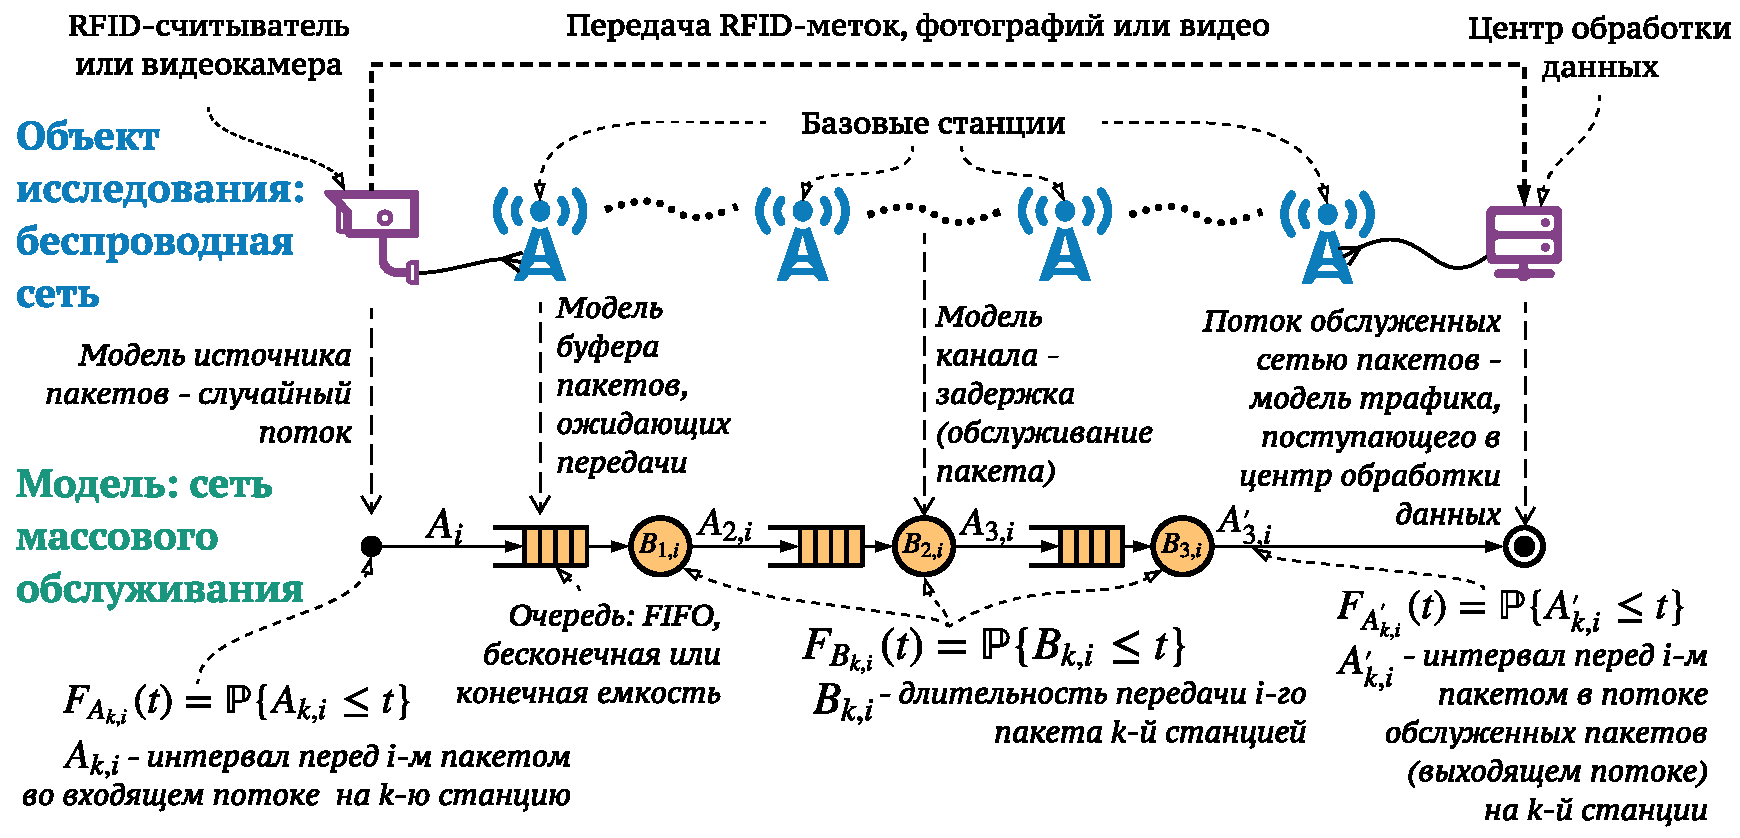
\includegraphics[width=1.0\textwidth]{chapter4/ch4_network_and_model}
  }
  \caption{Беспроводная сеть с линейной топологией и её аналитическая модель.}
  \label{fig:ch4_network_model}
\end{figure}

Для моделирования времени обслуживания будут использоваться PH-распределения $B_i \sim PH(S, \overline{\tau})$, а для моделирования интервалов между поступлениями в сеть пакетов "--- MAP-поток $A \sim MAP(D_0, D_1)$. Определения PH-распределений и MAP-потоков были даны в главе 1, а свойства, необходимые для вычисления характеристик тандемной сети массового обслуживания, будут приведены в следующем разделе.

Поставим формально задачу вычисления средней межконцевой задержки и вероятности потери пакетов из-за переполнения очередей в сети массового обслуживания. Пусть заданы длина сети (число узлов) $N$, емкость очередей $M$, входящий MAP-поток $X \sim MAP(D_0, D_1)$ и PH-распределения времени обслуживания $Y_k \sim PH(S_k, \overline{\tau}_k)$, $k = 1, 2, \dots, N$. Будем обозначать момент поступления $i$-го пакета на вход $k$-го узла как $t_{i,k}^{(a)}$, а момент завершения его обслуживания -- как $t_{i,k}^{(d)}$. Очевидно, что для любого $k < N$ выполняется $t_{i,k}^{(d)} = t_{i,{k+1}}^{(a)}$, если пакет не застает очередь $(k+1)$-го узла заполненной (в этом случае пакет теряется). Рассмотрим произвольный $i$-й пакет. Результатом обработки этого пакета может быть один из двух исходов: либо на некотором $k$-м узле пакет застанет очередь заполненной и будет отброшен, либо он будет обработан последовательно каждым из узлов, и покинет систему тогда, когда завершится его обработка последним узлом в момент $t_{i,N}^{(d)}$. Вероятность первого исхода (то есть потери пакета) будем обозначать $P_l$, она представляет собой долю пакетов, заставших какой-либо узел сети полностью заполненным. Для пакетов, которые не были потеряны, можно вычислить межконцевую задержку $\Delta t_i = t^{(d)}_{i,N} - t^{(a)}_{i,1}$.

Задача исследования состоит в поиске методов численной оценки средней межконцевой задержки $\overline{\Delta t}$ и вероятности потери пакета $P_l$.

Из-за экспоненциального роста размера пространства состояний при увеличении числа станций в сети, вычисление точных значений задержек и вероятностей потери пакетов возможно только для небольших сетей. Для получения оценок параметров в общем случае предлагается использовать метод редукции выходящих потоков, то есть заменять потоки обслуженных пакетов на выходе из очередного узла сети MAP-потоком небольшого размера. Этот метод будет подробно описан и численно исследован в этой главе диссертационной работы.

% На практике обычно известны только статистические оценки распределений или выборка интервалов между пакетами (например, полученная из сетевого дампа). Поэтому при выполнении численных экспериментов в качестве входных данных будем считать известными не сами матрицы $D_0, D_1, S, \overline{\tau}$, а моменты распределений. Пусть $m_a = \mathbb{E}X$ -- среднее время между поступлениями новых пакетов, $\sigma_a$ -- стандартное отклонение. Аналогично, пусть $m_s = \mathbb{E}Y$ -- среднее время обслуживания пакета, а $\sigma_s$ -- его стандартное отклонение. Время обслуживания будем задавать средним значением $m_s$, коэффициентом вариации $c_s = \sigma_s / m_s$ и коэффициентом асимметрии $\gamma_s = \mathbb{E}[(Y - m_s)^3] / \sigma_s^3$. Входящий поток будем задавать аналогично с помощью $m_a$, $c_a$ и $\gamma_a$, а также коэффициента автокорреляции между соседними интервалами $\rho_1$.


%%%%%%%%%%%%%%%%%%%%%%%%%%%%%%%%%%%%%%%%%%%%%%%%%%%%%%%%%%%%%%%%%%%%%%%%%%%%%%%%
\section{Открытая тандемная сеть массового обслуживания с узлами MAP/PH/1/M}\label{sec:ch4_queues}
%%%%%%%%%%%%%%%%%%%%%%%%%%%%%%%%%%%%%%%%%%%%%%%%%%%%%%%%%%%%%%%%%%%%%%%%%%%%%%%%

В этом разделе рассмотрим основные свойства PH-распределений, MAP-потоков и систем массового обслуживания MAP/PH/1/M. На базе этих свойств, сформулируем итерационный алгоритм, позволяющий рассчитывать характеристики сетей массового обслуживания типа MAP/PH/1/M $\rightarrow \bullet$/PH/1/M$\rightarrow \dots \rightarrow \bullet$/PH/1/M, и приведем анализ его сложности.


%%% ~~~~~~~~~~~~~~~~
\subsection{Свойства PH-распределений и MAP-потоков}\label{sec:ch4_queues_map_ph_props}
%%% ~~~~~~~~~~~~~~~~

Пусть $Y \sim PH(S, \overline{\tau})$, матрица $S$ и вектор $\overline{\tau}$ удовлетворяют ограничениям \eqref{eq:ch1_ph_def}. Тогда функция распределения $F(y)$ и моменты случайной величины $Y$ определяются как \cite{Buchholz2014}:

\begin{equation}
	\label{eq:ch4_ph_props}
	\begin{aligned}
		&F(y) = \mathbb{P}\{Y < y\} = 1 - \overline{\tau} e^{Sy} \mathbf{1}\\
		&\mathbb{E}Y^k = k! \overline{\tau} (-S)^{-k} \mathbf{1}
	\end{aligned}
\end{equation}

Пусть $X \sim MAP(D_0, D_1)$, где матрицы $D_0$ и $D_1$ удовлетворяют ограничениям \eqref{eq:ch1_map_def}. Матрица $D_1$ описывает переходы управляющей марковской цепи, сопровождающиеся генерацией пакетов (наблюдаемые переходы), а матрица $D_0$ "--- переходы, при которых генерации нового пакета не происходит (невидимые переходы). Если после генерации очередного пакета MAP-поток находится в состоянии $i$, время до появления следующего пакета имеет PH-распределние $X^{(i)} = PH(D_0, \overline{e}_i)$, где $\overline{e}_i = (0, \dots, 0, 1, 0, \dots, 0)$ "--- единичный вектор, в котором на $i$-й позиции стоит единица. Число состояний $W$ в управляющей цепи потока будем называть его размером или порядком и обозначать как $\vline X \vline$.

Функция распределения интервалов между событиями, значения моментов MAP-потока $X$ и коэффициенты корреляции с лагом $k$ определяются выражениям:

\begin{equation}
	\label{eq:ch4_map_props}
    \begin{aligned}
    \mathbb{P}\{X < t\} &= 1 - \overline{\alpha}e^{D_0 t}\overline{\mathbf{1}}\\
    \mathbb{E}X^{k} &= k! \overline{\alpha}(-D_0)^{-k}\overline{\mathbf{1}}\\
    \rho_k &= \frac{\lambda \overline{\pi} P^k (-D_0)^{-1} \overline{\mathbf{1}} - 1}{2 \overline{\pi} (-D_0)^{-1} \overline{\mathbf{1}} - 1}.
    \end{aligned}
\end{equation}
Здесь $P = (-D_0)^{-1} D_1$ "--- матрица вложенной цепи. Эта матрица $P$ и вектор стационарных вероятностей $\overline{\alpha}$ рассчитываются с помощью системы линейных алгебраических уравнений:

\begin{equation}
\label{eq:ch4_map_dtmc}
	\overline{\alpha}: \begin{cases}
		\overline{\alpha} P = \overline{\alpha} \\
		\sum\limits_{i=1}^{W} \alpha_i = 1
 	\end{cases}
\end{equation}

Стационарное распределение $\overline{\pi} \in \mathbb{R}^W$ вероятностей потока $MAP(D_0, D_1)$ является решением системы линейных уравнений:

\begin{equation}
	\label{eq:ch4_map_pmf}
	\begin{cases}
		\overline{\pi}(D_0 + D_1) &= \overline{\mathbf{0}}\\
		\overline{\pi}\overline{\mathbf{1}} &= 1
	\end{cases},
\end{equation}
где $\overline{\mathbf{0}}$ и $\overline{\mathbf{1}}$ "--- вектор-строки, состоящие из всех нулей и единиц соответственно.

Интенсивность MAP-потока можно найти как $\lambda = (\mathbb{E}X)^{-1}$. Её можно вычислить как математическое ожидание случайной величины, равной суммарной интенсивности наблюдаемых переходов:

\begin{equation}
	\label{eq:ch4_map_rate}
	\lambda = \sum\limits_{j=1}^{W} \pi_j \sum\limits_{k=1}^{W} \{D_1\}_{jk} = \overline{\pi} D_1 \overline{\mathbf{1}}
\end{equation}
Формула (\ref{eq:ch4_map_rate})~удобна, когда не требуется вычисление моментов старших порядков или коэффициентов автокорреляции, т.к. в этом случае также не требуется обращать матрицу $D_0$.

\begin{figure}[h]
    \centerfloat{
      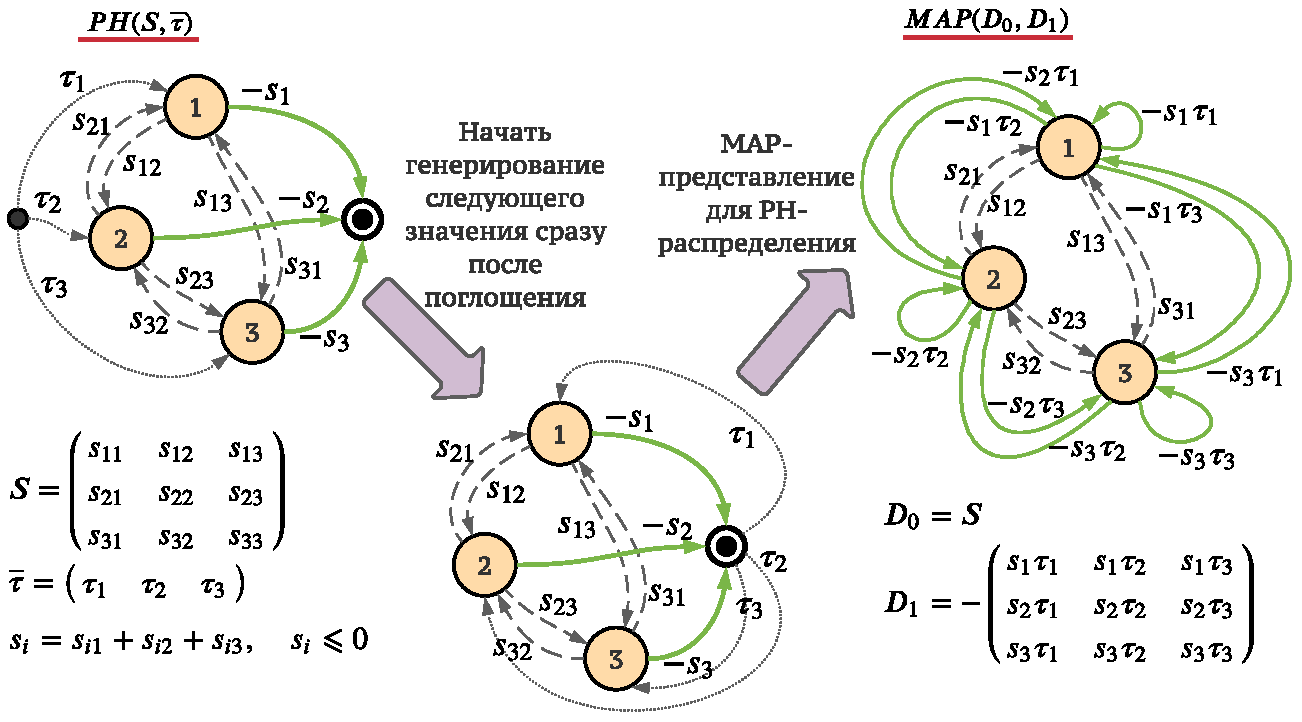
\includegraphics[width=1.0\textwidth]{chapter4/ch4_ph2map}
    }
    \caption{Пример построения MAP-потока, в котором все интервалы имеют одинаковое PH-распределение $PH(S, \overline{\tau})$ с тремя состояниями управляющей цепи.
    \label{fig:ch4_ph2map}}
\end{figure}

MAP-поток является обобщением над PH-распределением. Существенной чертой MAP-потока является то, что корреляция между интервалами может быть отличной от нуля (см. формулу~\eqref{eq:ch4_map_props}). В то же время, последовательность интервалов, каждый из которых имеет PH-распределение с одинаковыми параметрами $PH(S, \overline{\tau})$, также можно считать MAP-потоком, автокорреляция в котором будет нулевой. Для PH-распределения $PH(S, \overline{\tau})$ соответствующий MAP-поток будет иметь матрицы следующего вида:

\begin{equation}
    \label{eq:ch4_map_ph_representation}
    D_0 = S, \qquad D_1 = (-S \overline{1}) \overline{\tau} = -\left(
        \begin{matrix}
            s_1\\
            s_2\\
            \vdots\\
            s_V
        \end{matrix}
     \right) \left(
         \begin{matrix}
            \tau_1 & \tau_2 & \dots &
         \end{matrix}
     \right),
\end{equation}
где $s_i = \sum_{j=1}^V s_{ij}$
Пример построения MAP-потока по PH-распределению приведен на рис.~\ref{fig:ch4_ph2map}.



%%% ~~~~~~~~~~~~~~~~
\subsection{Свойства системы MAP/PH/1/M}\label{sec:ch4_queue_net_system_props}
%%% ~~~~~~~~~~~~~~~~

Ключевое свойство систем массового обслуживания MAP/PH/1/M, благодаря которому их удобно использовать для моделирования многошаговых сетей -- замкнутость на множестве MAP-потоков: согласно следующим теоремам (см. \cite{VishnevskyDudin2018}), результат просеивания MAP-потока "--- MAP-поток, сумма MAP-потоков "--- MAP-поток, и поток обслуженных заявок, выходящих из системы MAP/PH/1/M, также является также MAP-потоком. В дальнейшем будем обозначать выходной поток $Z$ из системы массового обслуживания с входным потоком $X$, временем обслуживания $Y$ и емкостью очереди $M$ как $\mathcal{D}(X, Y, M)$.

\begin{thm}\label{th:ch4_sifted_map}\textnormal{\cite{VishnevskyDudin2018}}
  Результат просеивания MAP-потока $X \sim MAP(D_{0},D_{1})$ с вероятностью $p$ "--- MAP-поток $X_{p} \sim MAP(D_{0}+(1-p)D_{1},pD_{1})$ (в дальнейшем обозначается как $pX$)
\end{thm}

\begin{thm}\label{th:ch4_maps_sum}\textnormal{\cite{VishnevskyDudin2018}}
  Сумма MAP-потоков $X_{1}$ и $X_{2}$, $X_i \sim MAP(D_{0}^{(i)},D_{1}^{(i)})$, $i=1,2$ "--- MAP-поток $X$:
  $$
    X = X_{1} \oplus X_{2} \sim MAP(D_{0}^{(1)} \oplus D_{0}^{(2)},D_{1}^{(1)} \oplus D_{1}^{(2)}),
  $$
  где $\oplus$ "--- сумма Кронекера.
\end{thm}

\textbf{Замечание.} Если потоки $X_1$ и $X_2$ имеют размерности $W_1$ и $W_2$, то размерность суммарного потока $X$ равняется $W = W_1 W_2$.

\begin{thm}\label{th:ch4_map_departure}\textnormal{\cite{VishnevskyDudin2018}}
    Пусть в системе MAP/PH/1/M $X \sim MAP(D_{0}$ $D_{1})$, $D_i \in \mathbb{R}^{W \times W}, i=0,1$ -- входящий поток, $Y \sim PH(S, \overline{\tau})$, $\mathbb{R}^{V \times V}$ -- время обслуживания, обслуживание ведется согласно дисциплине FIFO, а ёмкость очереди равна $M$. Тогда поток выходящих (обслуженных) пакетов есть MAP-поток $Z \sim MAP(D'_{0},D'_{1})$, матрицы которого определяются как:
    \begin{equation}
        \label{eq:ch4_qs_departure_d0}
        D'_{0} =
        \begin{bmatrix}
            D_{0} \otimes I_{V} & D_{1}\otimes (\overline{\tau} \otimes \overline{\mathbf{1}}_{V}) & 0 & \cdots & 0 & 0\\
            0 & D_{0} \otimes S & D_{1} \otimes I_{V} & \cdots & 0 & 0\\
            0 & 0 & D_{0} \otimes S & \cdots & 0 & 0 \\
            \vdots & \vdots & \vdots & \ddots & \vdots & \vdots \\
            0 & 0 & 0 & \cdots & D_{0} \otimes S & D_{1} \otimes I_{V}\\
            0 & 0 & 0 & \cdots & 0 & (D_{0}+D_{1}) \otimes S
        \end{bmatrix},
    \end{equation}
    \begin{equation}
        \label{eq:ch4_qs_departure_d1}
        D'_{1} =
          \begin{bmatrix}
              0 & \cdots & 0 & 0 \\
              I_{W} \otimes C_{t} & \cdots & 0 & 0 \\
              \vdots & \ddots & \vdots & \vdots \\
              0 & \cdots & 0 & I_{W} \otimes C_{t} & 0
          \end{bmatrix},
    \end{equation}
    где $C_{t} = (-S \overline{\mathbf{1}}_{V}) \otimes \overline{\tau}$, а $I_V$, $I_W$ -- едининые матрицы порядка $V$ и $W$ соответственно.
\end{thm}

Из структуры матриц потока $Z$ можно сделать следующие выводы. Во-первых, поток $Z$ имеет размерность $|Z| = (M+2)|X| |Y| = (M+2) V W$. Во-вторых, каждому состоянию потока $Z$ соответствует некоторое число пакетов в системе и состояния входящего MAP-потока $X$ и обслуживающего прибора $Y$. Пусть управляющая цепь потока $Z$ находится в состоянии $n$. Тогда в системе $\lfloor \frac{n}{VW} \rfloor$ пакетов, входящий MAP-поток находится в состоянии $\lfloor \frac{n (\mathbf{mod}\;VW)}{V} \rfloor + 1$, а обслуживающий прибор -- в состоянии $n(\mathbf{mod} V)+1$.

Предыдущее замечание можно обощить. По сути, при построении матриц выходящего MAP-потока производится построение марковской цепи, управляющей работой системы MAP/PH/1/M. Действительно, в такой системе переходы происходят из-за возникновения одного из двух событий: переход в цепи входящего MAP-потока или переход в цепи PH-распределения. При этом, если переход в цепи входящего потока сопровождается формированием сообщения, и система не находится в состоянии полностью заполненной очереди, то размер системы увеличивается. Если же переход происходит в цепи PH-распределения в поглощающее состояние, то размер системы уменьшается на единцицу. Элементы матрицы $D'_0$ соответствуют всем переходам, кроме поглощения в цепи PH-распределения, последним же соответствуют элементы матрицы $D'_1$. По этой причине, когда будет требоваться найти распределение вероятностей управляющей цепи системы MAP/PH/1/M, будем использовать инфинитезимальый генератор управляющей цепи выходящего потока $Z$.

Обозначим $\overline{\pi}$ стационарное распределение $X$, а $\overline{\theta}$ стационарное распределение $Z$. Вектор $\overline{\theta}$ можно переписать в виде $\overline{\theta} = (\overline{\theta}_0, \overline{\theta}_1, \dots, \overline{\theta}_{M+1})$, где $\overline{\theta}_k$ "--- часть вектора $\overline{\theta}$, соответствующая тем состояниям системы, в которых число пакетов равно $k$. Пусть $\mu(t)$ "--- случайный процесс, значение которого в каждый момент времени равняется числу пакетов в системе. Обозначим $p_k = \lim\limits_{t \rightarrow \infty} \mathbb{P}\{\mu(t) = k\}$ "--- стационарная вероятность того, что в системе $k=\overline{0,M+1}$ пакетов. Тогда, зная стационарное распределение $\overline{\theta}$ управляющей цепи MAP-потока $Z$, можно вычислить распределение $\overline{p}$:

\begin{equation}
	\label{eq:ch4_qs_size_pmf}
	p_k = \sum\limits_{j=1}^{VW} \{ \overline{\theta}_k \}_j.
\end{equation}
Отсюда можно рассчитать среднее число пакетов в системе как $m_1 = \mathbb{E}\mu$:

\begin{equation}
  \label{eq:ch4_qs_size_avg}
  \begin{aligned}
	  m_1 = \sum\limits_{k=0}^{M+1} k \mathbb{P}\{\mu = k\} = \sum\limits_{k=0}^{M+1} k p_k = \sum\limits_{k=0}^{M+1} k \sum\limits_{j=1}^{VW} \{ \overline{\theta}_k \}_j = \sum\limits_{k=0}^{M+1} \sum\limits_{j=1}^{VW} k \theta_{kVW+j}\hfill.
  \end{aligned}
\end{equation}

Для получения вероятности потери пакета из-за переполнения очереди нужно более подробно рассмотреть часть вектора $\overline{\theta}$, соответствующую случаю заполненной очереди (т.е. $\mu=M+1$). Состояния внутри блоков матриц \eqref{eq:ch4_qs_departure_d0} и \eqref{eq:ch4_qs_departure_d1} сгруппированы по состояниям входящего MAP-потока, т.е. состояния $\{ \overline{\theta}_k \}_{jV + 1}, \dots \{ \overline{\theta}_k \}_{(j+1)V}$ соответствуют всевозможным состояниям цепи PH-распределения и состоянию $j$ входящего MAP-потока, когда в системе $k$ пакетов. Определим:

\begin{equation}
    \label{eq:ch4_qs_size_slice_pmf}
    \overline{\psi}_k = ( \sum\limits_{j=1}^{V}\{ \overline{\theta}_k \}_j, \dots, \sum\limits_{j=1}^{V}\{ \overline{\theta}_{k} \}_{(W-1)V + j} )
\end{equation}
"--- распределение вероятностей входящего MAP-потока при $k$ пакетах в системе. Тогда вероятность $P_L$ потери пакета можно выразить так:

\begin{equation}
  \label{eq:ch4_qs_loss_prob}
  P_L = \overline{\psi}_{M+1} \frac{D_1}{\lambda_X}\overline{\mathbf{1}}
\end{equation}

Наконец, зная интенсивность входящего потока $\lambda_{X}$, среднее число пакетов в системе $m_1$ и вероятность потери пакетов $P_L$, используя формулу Литтла, можно рассчитать среднюю задержку:

\begin{equation}
	\label{eq:ch4_qs_delay}
	T = \frac{m_1}{(1 - P_L)\lambda_{X}}.
\end{equation}
Множитель $(1 - P_L)$ в знаменателе возникает в следствие того, что из-за переполнения очереди лишь часть пакетов входящего потока попадает в систему, т.е. фактическая интенсивность потока пакетов, поступающих в систему, составляет $(1 - P_L) \lambda_{X}$.



%%% ~~~~~~~~~~~~~~~~
\subsection{Точный расчёт характеристик сети массового обслуживания}\label{sec:ch4_queue_net_precise}
%%% ~~~~~~~~~~~~~~~~


Используя формулы \eqref{eq:ch4_qs_size_avg}, \eqref{eq:ch4_qs_loss_prob} и \eqref{eq:ch4_qs_delay} несложно вычислить среднюю межконцевую задержку пакетов в сети и вероятность потери пакета на каком либо узле. Будем рассматривать два варианта сетей: сети с кросс-трафиком, в которых потоки данных поступают на каждый узел, и сети без кросс-трафика, в которых внешний трафик поступает только на первую станцию, и все последующие станции передают только его.

\begin{figure}[htb]
	\centerfloat{
    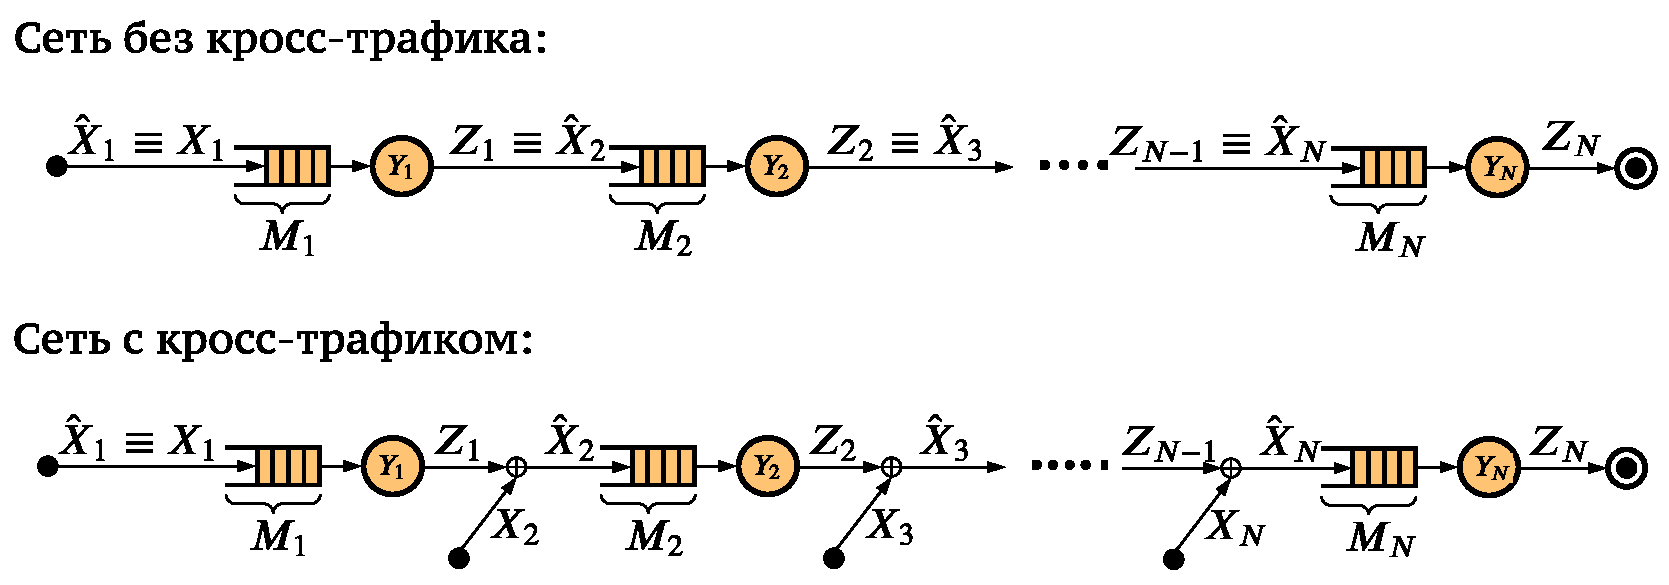
\includegraphics[width=0.95\textwidth]{chapter4/ch4_queueing_networks}
  }
  \caption{Сети массового обслуживания с кросс-трафиком и без него.}
  \label{fig:ch4_queueing_networks}
\end{figure}

Пусть в сети (см. рис. \ref{fig:ch4_queueing_networks}) $N$ станций, емкость очереди на $i$-й станции ($i = 1,2, \dots, N$) равна $M_i \in \mathbb{N}$, а длительность обслуживания $Y_i$ имеет PH-распределение $Y_i \sim PH(S_i, \overline{\tau})$, $S_i \in \mathbb{R}^{V_i \times V_i}$, $V_i \in \mathbb{N}$. Если в сети есть кросс-трафик, то на каждую станцию поступает пользовательский поток $X_i \sim MAP(D_{0,i}, D_{1,i})$; если кросс-трафика нет, то поток $X_1 \equiv X = MAP(D_0, D_1)$ поступает только на первую станцию. Обозначим порядок входящего MAP-потока на $i$-ю станцию как $W_i$, то есть $D_{0,i}, D_{1,i} \in \mathbb{R}^{W_i \times W_i}$, $W_i \in \mathbb{N}$.

Обозначим $Z_i$ - выходящий MAP-поток с $i$-й станции, а $\hat{X}_i$ - общий входящий поток на $i$-ю станцию. Тогда, согласно теоремам \ref{th:ch4_maps_sum} и \ref{th:ch4_map_departure}, потоки $\hat{X}_i$ и $Z_i$ "--- MAP-потоки. Используя ранее введённые обозначения, их можно определить формально следующим образом:

\begin{equation}
  \label{eq:ch4_total_arrival_and_departure}
  \begin{aligned}
    \hat{X}_1 &\equiv X_1\\
    \hat{X}_i &= \begin{cases}
      X_i \oplus Z_{i-1},&\text{в сети есть кросс-трафик и } i = 2,3, \dots, N\\
      Z_{i-1},&\text{в сети нет кросс-трафика}
    \end{cases}\\
    Z_i &= \mathcal{D}(\hat{X}_i, Y_i, M)
  \end{aligned}
\end{equation}

Обозначим порядок выходящих MAP-потоков $Z_i$ как $U_i$, $i=1,2,\dots N$, то есть $Z_i \sim MAP(\tilde{D}_{i,0}, \tilde{D}_{i,1})$ и $\tilde{D}_{i,0}, \tilde{D}_{i,1} \in \mathbb{R}^{U_i \times U_i}$. Тогда величина $U_i$ определяется с помощью следующего утверждения.

\begin{prop}\label{prop:ch4_departure_order}
	Порядок $U_i$ MAP-потока обслуженных пакетов $Z_i$ на выходе из $i$-го узла, $i = 1,2,\dots N$, определяется как:
	$$
	U_i = \begin{cases}
		\prod\limits_{j=1}^{i}(M_j + 2)V_jW_j,&\text{если в сети есть кросс-трафик}\\
		W_1\prod\limits_{j=1}^{i}(M_j + 2)V_j,&\text{если кросс-трафика нет}.
	\end{cases}
	$$
\end{prop}
\begin{proof}
Утверждение доказывается по индукции. При $i = 1$ $Z_1 = \mathcal{D}(X_1, Y_1, M_1)$ и $U_1 = (M_1 + 2)V_1W_1$ согласно замечанию к теореме \ref{th:ch4_map_departure}.

Пусть утверждение верно при $i = n-1$. Если в сети нет кросс-трафика, то $Z_i = \mathcal{D}(\hat{X}_i, Y_i, M_i) = \mathcal{D}(Z_{i-1}, Y_i, M_i)$ и величина $U_i$ определяется как:
$$
  \begin{aligned}
    U_i &= (M_i + 2) V_i U_{i-1} = (M_i + 2) V_i \times (W_1 \prod\limits_{j=1}^{i-1}(M_j + 2)V_j)\\
    &= W_1 \prod\limits_{j=1}^{i}(M_j + 2)V_j.
  \end{aligned}
$$
Если же в сети есть кросс-трафик, то
$$
  Z_i = \mathcal{D}(\hat{X}_i, Y_i, M_i) = \mathcal{D}(Z_{i-1} \oplus X_i, Y_i, M_i),
$$
и порядок потока $Z_i$ определяется следующей цепочкой равенств:
$$
  \begin{aligned}
    U_i &= (M_i + 2) V_i (U_{i-1} W_i) = (M_i + 2) V_i W_i \times \prod\limits_{j=1}^{i-1}(M_j + 2) V_j W_j)\\
    &= \prod\limits_{j=1}^{i}(M_j + 2) V_j W_j.
  \end{aligned}
$$
\end{proof}

Схема расчёта характеристик сети выглядит следующим образом.

\textit{Шаг 1.} Положим $i := 1$.

\textit{Шаг 2.} Если $i = 1$, то положим $\hat{X}_i = X_1$. Если же $i > 1$, то вычисляем $\hat{X}_i$ согласно \eqref{eq:ch4_total_arrival_and_departure}: $\hat{X}_i = Z_{i-1}$, если в сети нет кросс-трафика, и $\hat{X}_i = Z_{i-1} \oplus X_i$ иначе. Обозначим матрицы потока $\hat{X}_i$ как $\hat{D}_{i,0}$ и $\hat{D}_{i,1}$, то есть $\hat{X}_i = MAP(\hat{D}_{i,0}, \hat{D}_{i,1})$.

\textit{Шаг 3.} С помощью теоремы \ref{th:ch4_map_departure} вычисляем матрицы $D'_{i,0}$, $D'_{i,1}$ MAP-потока $Z_i = \mathcal{D}(\hat{X}_i, Y_i, M_i)$.

\textit{Шаг 4.} Для выходящего MAP-потока $Z_i$ вычисляем его стационарное распределение $\overline{\theta}^{(i)}$ с помощью системы линейных алгебраических уравнений:
$$
  \begin{cases}
	  \overline{\theta}^{(i)}(D'_{i,0} + D'_{i,1}) &= 0\\
	  \overline{\theta}^{(i)} \mathbf{1} &= 1
  \end{cases}
$$

\textit{Шаг 5.} Рассчитываем среднее число пакетов в очереди $i$-й станции согласно \eqref{eq:ch4_qs_size_avg}:
$$
  m_1^{(i)} = \sum\limits_{k=0}^{M_i + 1} k \sum\limits_{j=1}^{V_i \hat{W}_i} \theta^{(i)}_{k V_i \hat{W}_i + j}\;,
$$
где $V_i = |Y_i|$ "--- порядок PH-распределения $Y_i$, а $\hat{W}_i = |\hat{X}_i|$ "--- порядок входящего MAP-потока $\hat{X}_i$.

\textit{Шаг 6.} Определяем стационарное распределение вероятностей $\overline{\pi}^{(i)}$ входящего потока $\hat{X}_i$. Если в сети нет кросс-трафика и $i > 1$, то полагаем $\overline{\pi}^{(i)} \equiv \overline{\theta}^{(i-1)}$. В противном случае находим $\overline{\pi}^{(i)}$ как решение системы линейных алгебраических уравнений:
$$
  \begin{cases}
	  \overline{\pi}^{(i)}(\hat{D}_{i,0} + \hat{D}_{i,1}) &= 0\\
	  \overline{\pi}^{(i)} \mathbf{1} &= 1
  \end{cases}
$$

\textit{Шаг 7.} С помощью найденного на предыдущем шаге стационарного распределения $\overline{\pi}^{(i)}$ входящего потока $\hat{X}_i$ и формулы \eqref{eq:ch4_map_rate} вычисляем интенсивность поступления пакетов на $i$-ю станцию:
$$
  \lambda_i = \overline{\pi}^{(i)} \hat{D}_{i,1} \overline{\mathbf{1}}.
$$

\textit{Шаг 8.} Рассчитываем распределение состояний входящего MAP-потока при наличии в системе $M_i + 1$ пакета (то есть при заполненной системе):
$$
  \overline{\psi}^{(i)} = \left(
  \sum\limits_{j=1}^{V_i} \{ \overline{\theta}^{(i)}_{M_i+1} \}_j,
  \dots,
  \sum\limits_{j=1}^{V_i} \{ \overline{\theta}^{(i)}_{M_i+1} \}_{(\hat{W}_i-1) V_i + j}
  \right).
$$
Здесь вектор $\overline{\theta}_{M_i+1}^{(i)}$ "--- часть вектора $\overline{\theta}^{(i)}$, относящаяся к состояниям системы, когда в ней находится $M_i + 1$ пакет.

\textit{Шаг 9.} Вычисляем векроятность потери пакета из-за переполнения $i$-й очереди с помощью~\eqref{eq:ch4_qs_loss_prob}:
$$
  P_L^{(i)} = \overline{\psi}^{(i)} \frac{\hat{D}_{i,0}}{\lambda_i} \overline{\mathbf{1}}.
$$

\textit{Шаг 10.} Вычисляем среднюю задержку пакетов на $i$-й станции с помощью~\eqref{eq:ch4_qs_delay}:
$$
  T_i = \frac{m_1^{(i)}}{(1 - P_L^{(i)}) \lambda_i}
$$

\textit{Шаг 11.} Если $i < N$, то увеличиваем $i := i + 1$ и переходим на шаг 2. В противном случае переходим далее, на шаг 12.

\textit{Шаг 12.} Вычисляем вероятность потери пакета $P_L = \prod\limits_{i=1}^{N} (1 - P_L^{(i)})$.

\textit{Шаг 13.} Вычисляем общую задержку $T = \sum\limits_{i=1}^{N} T_i$.

Предложенная схема проста в вычислении. По сути, на каждом шаге с помощью нескольких операций произведения Кронекера строятся блочные матрицы для выходящего MAP-потока, а также, если в сети есть кросс-трафик, с помощью суммы Кронекера строятся матрицы входящего потока. Далее решаются две (если в сети есть кросс-трафик) или одна (в противном случае) системы линейных алгебраических уравнений для определения стационарных вероятностей входящего и исходящего потока. Наконец, с помощью нескольких операций умножений найденных распределений на матрицы потоков, вычисляются искомые характеристики "--- вероятность потери пакета, средний размер системы и задержка.

Главный недостаток этой схемы расчета "--- чрезвычайно высокая вычислительная сложность.

\begin{prop}\label{prop:ch4_base_algorithm_complexity}
  Пусть входящие MAP-потоки имеют порядок $W$, PH-распределения "--- порядок $V$, ёмкость очередей равна $M$, и сеть содержит $N$ станций. Тогда итерационная схема расчета характеристик тандемной сети имеет сложность:
  \begin{itemize}
	  \item $O((M V W)^{3N})$, если в сети есть кросс-трафик
	  \item $O(W^3 (M V)^{3N})$, если кросс-тррафика в сети нет.
  \end{itemize}
\end{prop}
\begin{proof}
Рассмотрим $i$-ю итерацию алгоритма, $i \leqslant N$, то есть расчёт характеристик $i$-й станции сети. Отметим сперва, что при $i > 1$ порядок выходящего потока с предыдущей $i-1$-й станции есть $(M + 2) V \hat{W}_i$, где $\hat{W}_i$ "--- порядок входящего потока на $i$-ю станцию. Согласно \ref{prop:ch4_departure_order}, при наличии в сети кросс трафика $U_i = ((M+2)VW)^i$, а если кросс-трафика нет, то $U_i = W((M+2)V)^i$.

Сложность итерации определяется шагами 4 и 6, в которых необходимо решать системы линейных алгебраических уравнений, причем порядок матрицы системы на шаге 4 (генератор выходящего потока) заведомо выше, чем системы на шаге 6 (генератор входящего потока). Полагая, что для решения системы используется алгоритм наподобии метода Гаусса, на шаге 4 потребуется $O(U_i^3)$ операций. Остальные шаги имеют более низкую сложность: шаги 1, 10 и 11 "--- $O(1)$, шаг 2 "--- $O(U_{i-1}^2 W^2)$, шаг 3 "--- $O(U_i^2)$, шаг 5 "--- $O(VW + M)$, шаги 7 и 9 "--- $O(U_i^2)$, шаг 8 "--- $O(VM)$. Сложность шагов 12 и 13 есть $O(N)$.

Таким образом, если в сети есть кросс-трафик, сложность алгоритма составит
$$
  \begin{aligned}
    O((VWM)^3) &+ O((VWM)^6) + \dots + O((VWM)^{3N}) + O(N) \\
    &= O(VWM)^{3N},
  \end{aligned}
$$
а если кросс-трафика в сети нет, то
$$
  \begin{aligned}
    O(W^3 (VM)^3) &+ O(W^3 (VM)^6) + \dots + O(W^3 (VM)^{3N}) + O(N) \\
    &= O(W^3 (VM)^{3N}).
  \end{aligned}
$$

\end{proof}

\textbf{Замечание 1.} Учитывая, что матрицы выходящего потока $Z_i$ имеют блочный трехдиагональный вид, они будут сильно разрежены. Благодаря этому можно попытаться применить более эффективные способы решения системы алгебраических уравнений. Однако, показатель степени в оценке сложности все равно не окажется ниже, чем $(2 + \epsilon) N$.


На практике утверждения \ref{prop:ch4_departure_order} и \ref{prop:ch4_base_algorithm_complexity} означают, что искать решения с помощью представленной схемы вычислений становится невозможным даже при относительно небольших $N$, $V$ и $W$. В таблице \ref{table:ch4_map_order_growth} приведены примеры роста порядков для различных порядков входящих процессов и времен обслуживания.

\begin{table}[h!]
\centering
\begin{tabular}{ |c|c|c||c|c|c|c|c| }
\hline
\multicolumn{3}{|c||}{} & \multicolumn{5}{c|}{Номер станции} \\
\hline
%\multirow{2}{4em}{Сеть без кросс-трафика, число станций}\\
$W$ & $V$ & $M$ & 1 & 2 & 3 & 4 & 5\\
\hline
\multicolumn{8}{|c|}{Сети без кросс-трафика} \\
\hline
1 & 1 & 1 & 3 & 9 & 27 & 81 & 243 \\
1 & 1 & 3 & 5 & 25 & 125 & 625 & 3'125 \\
2 & 2 & 2 & 16 & 128 & 1'024 & 8'192 & 65'536 \\
3 & 1 & 3 & 15 & 75 & 375 & 1'875 & 9'375 \\
1 & 3 & 3 & 15 & 225 & 3'375 & 50'625 & 759'375 \\
3 & 3 & 3 & 45 & 675 & 10'125 & 151'875 & 2'278'125 \\
\hline
\multicolumn{8}{|c|}{Сети с кросс-трафиком} \\
\hline
1 & 1 & 1 & 3 & 9 & 27 & 81 & 243 \\
1 & 1 & 3 & 5 & 25 & 125 & 625 & 3'125 \\
2 & 2 & 2 & 16 & 256 & 4'096 & 65'536 & 1'048'576 \\
3 & 1 & 3 & 15 & 225 & 3'375 & 50'625 & 759'375 \\
1 & 3 & 3 & 15 & 225 & 3'375 & 50'625 & 759'375 \\
3 & 3 & 3 & 45 & 2'025 & 91'125 & 4'100'625 & 184'528'125 \\
\hline
\end{tabular}
\caption{Порядки выходящих MAP-потоков в зависимости от порядков PH-распределения ($V$), входящих MAP-потоков ($W$) и ёмкости очереди ($M$).\label{table:ch4_map_order_growth}
}
\end{table}

Таким образом, для практического применения открытых сетей с узлами MAP/PH/1/M необходимы более эффективные методы расчета, пусть даже их результаты будут приближенными.




%%%%%%%%%%%%%%%%%%%%%%%%%%%%%%%%%%%%%%%%%%%%%%%%%%%%%%%%%%%%%%%%%%%%%%%%%%%%%%%%
\section{Расчёт характеристик сети массового обслуживания методом Монте-Карло}
%%%%%%%%%%%%%%%%%%%%%%%%%%%%%%%%%%%%%%%%%%%%%%%%%%%%%%%%%%%%%%%%%%%%%%%%%%%%%%%%

Расчёт методом Монте-Карло заключается в многократном проигрывании прохождения пакетов по сети массового обслуживания и замерах длительностей их пребывания в узлах, длин очередей и потерь. Для реализации этого метода лучше всего подходят системы дискретно-событийного моделирования, в которых обрабатываются возникающие события, а время изменяется только в начале обработки очередного события.

Методы и алгоритмы имитационного моделирования открытых сетей массового обслуживания хорошо известны, поэтому далее приведем лишь краткое схематичное описание работы модели и способа расчёта характеристик сети.

Для моделирования сети с узлами MAP/PH/1/M нужно описать обработку двух типов событий: появление нового пакета во входящем MAP-потоке и завершение обработки пакета на узле.

Пусть, как и ранее, $N$ "--- число станций в сети. Обозначим $K$ "--- глобальный счетчик пакетов, $T_k^a$ "--- время появления $k$-го пакета, $\Delta$ "--- множество вычисленных задержек, $a_i$ "--- число сгенерированных пакетов из $i$-го потока, $l_i$ "--- число потерянных пакетов на $i$-й станции, $t$ "--- модельное время, $n_i$ "--- число пакетов на $i$-й станции.

Если какая-либо из перечисленных величин $\chi$ будет нас интересовать в определенный момент модельного времени $t$, то будем писать $\chi(t)$. Кроме того, при описании операций будем использовать запись $\chi' := f(\chi)$, подразумевая, что после завершения выполнения текущего действия величина $\chi$ примет значение $\chi'$, а до окончания операции она сохраняет значение $\chi$.


%%% ~~~~~~~~~~~~~~~~
\subsection{Обработка событий}
%%% ~~~~~~~~~~~~~~~~

При \textbf{инициализации} модели для каждого потока $X_i$ выбирается интервал до поступления первого пакета $\tau_i$, и на время $\tau_i$ назначается обработка события поступления пакета на $i$-ю станцию.

Рассмотрим действия, происходящие при возникновении событий поступления нового пакета и завершении обслуживания.

\textbf{Обработка поступления нового пакета.} Если в момент времени $t = t_0$ во входящем потоке, поступающем в узел с номером $i$, происходит появление пакета, выполняются следующие действия.

\textit{Шаг 1.} Пакет обрабатывается в зависимости от того, занят ли прибор и есть ли место в очереди:
\begin{itemize}
  \item Если $n_i = 0$, то есть обслуживающий прибор узла $i$ свободен, то вычисляется случайная длительность обслуживания $\tau_s$, $\mathbb{P}\{\tau_s \leqslant \tau\} = F_{Y_i}(\tau)$, на момент времени $t_0 + \tau_s$ назначается событие окончания обслуживания на $i$-м приборе, а число пакетов в системе увличивается на единицу: $n'_i := n_i + 1$.
  \item Если $1 \leqslant n_i \leqslant M_i$, то есть обслуживающий прибор занят, но в очереди есть место, то пакет помещается в очередь, и счётчик числа пакетов в системе увличивается на единицу: $n'_i := n_i + 1$.
  \item Если $n_i = M_i + 1$, то есть в очереди нет места, пакет теряется, а счётчик потерянных пакетов $l_i$ увеличивается на единицу: $l'_i := l_i + 1$.
\end{itemize}

\textit{Шаг 2.} Для пакета сохраняется время его появления $T_K^a := t_0$.
\textit{Шаг 3.} Счётчики числа сгенерированных пакетов $K$ и $a_i$ увеличиваются на единицу: $K' := K + 1$, $a'_i := a_i + 1$.
\textit{Шаг 4.} Выбирается случайное время до следующего появления пакета в $i$-м потоке $\tau_a$, $\mathbb{P}\{ \tau_a \leqslant \tau \} = F_{X_i}(\tau)$, на момент $t_0 + \tau_a$ назначается следующее событие появления нового пакета в $i$-м потоке.

\textbf{Завершение обслуживания пакета.} Если в момент времени $t_0$ завершается обслуживание $k$-го пакета в узле $i$, то выполняется следующее:

\textit{Шаг 1.} Если $i < N$, то пакет обрабатывается в зависимости от того, занят ли прибор на следующей станции, и есть ли место в её очереди:
\begin{itemize}
\item Если $n_{i+1} = 0$, то есть обслуживающий прибор узла $i+1$ свободен, то вычисляется случайная длительность обслуживания $\tau_s$, $\mathbb{P}\{\tau_s \leqslant \tau\} = F_{Y_{i+1}}(\tau)$, на момент времени $t_0 + \tau_s$ назначается событие окончания обслуживания на $i+1$-м приборе, а число пакетов в системе увеличивается на единицу: $n'_{i+1} := n_{i+1} + 1$.
\item Если $1 \leqslant n_{i+1} \leqslant M_{i+1}$, то есть обслуживающий прибор занят, но в очереди есть место, то пакет помещается в очередь $i+1$-й станции и увеличивается счётчик числа пакетов в системе: $n'_{i+1} := n_{i+1} + 1$.
\item Если $n_{i+1} = M_{i+1}$, то есть в очереди нет места, то пакет теряется, а счётчик потерянных пакетов $l_{i+1}$ увеличивается на единицу: $l'_{i+1} := l_{i+1} + 1$.
\end{itemize}

\textit{Шаг 2.} Если $i = N$, то в $\Delta$ добавляется величина $t_0 - T_k^a$, то есть время с появления пакета до натоящего времени.
\textit{Шаг 3.} Число пакетов на $i$-й станции уменьшается: $n'_i := n_i - 1$.
\textit{Шаг 4.} Если в очереди $i$-й станции есть еще пакеты, то есть $n_i > 0$, то вычисляется случайная длительность обслуживания $\tau_s$, $\mathbb{P}\{\tau_s \leqslant \tau\} = F_{Y_i}(\tau)$, на момент времени $t_0 + \tau_s$ назначается событие окончания обслуживания на $i$-м приборе.



%%% ~~~~~~~~~~~~~~~~
\subsection{Расчет характеристик}
%%% ~~~~~~~~~~~~~~~~

В момент времени $t$ межконцевую среднюю задержку $\overline{T}(t)$ можно оценить как
$$
\overline{T}(t) = \frac{1}{|\Delta(t)|}\sum\limits_{\delta \in \Delta(t)} \delta,
$$
а вероятность успешной доставки пакета $P_s(t)$ "--- как долю доставленных пакетов из всех пакетов, успевших к моменту времени $t$ покинуть систему.
$$
P_s(t) = 1 - \frac{\sum\limits_{i=1}^{N} l_i(t)}{K(t) - \sum\limits_{i=1}^{N} n_i}
$$

Симуляция производится либо до достижения модельным временем заданного значения $T_{max}$, либо до того, как отклонение искомых характеристик не становится меньше заданной величины $\epsilon$. Для реализации последнего критерия, можно вычислять оценки $\overline{T}(t)$ и $P_s(t)$ в моменты модельного времени $t_1, t_2, \dots$ и останавливать симуляцию в момент времени $t_n$, если $\left(\overline{T}(t_n) - \overline{T}(t_{n-1}) \right) / \overline{T}(t_n) < \epsilon$ и $\left( P_s(t_n) - P_s(t_{n-1}) \right) / P_s(t_{n-1}) < \epsilon$.

Для повышения достоверности результатов можно провести симуляцию несколько раз, и в качестве результатов эксперимента использовать усреднённые значения по всем проведённым симуляциям.



%%% ~~~~~~~~~~~~~~~~
\subsection{Программная реализация}
%%% ~~~~~~~~~~~~~~~~

Выбор конкретных алгоритмов и методов реализации имитационной модели зависит от того, используется ли готовая система имитационного моделирования, или же модель пишется без использования готовых систем. Пакеты для моделирования систем массового обслуживания входят в такие системы, как OMNeT++, MatLab, AnyLogic и другие.

В диссертационном исследовании автором была разработана высокоэффективная реализацию модели сети с MAP-потоками и PH-распределениями на языке C++, и разработан интерфейс для ее подключения в код на Python с помощью Cython. Реализация модели, а также все приведенные в исследовании численные эксперименты, доступны на GitHub: \url{https://github.com/larioandr/thesis-queues}. Все алгоритмы для расчета характеристик в имитационной модели реализованы так, чтобы использовать ограниченный объем памяти. Кроме реализации имитационной модели, пакет содержит классы для представления MAP-потоков, PH-распределений, систем MAP/PH/1/M и методы для аналитического расчета их характеристик.


%%% ~~~~~~~~~~~~~~~~
\subsection{Преимущества и недостатки метода}
%%% ~~~~~~~~~~~~~~~~
Главное преимущество метода Монте-Карло для вычисления характеристик сети массового обслуживания "--- его простота. Так как при выполнении модели не происходит явного построения выходных потоков, нет и экспоненциального роста размера задачи при увеличении числа станций. Точность получаемых результатов связана только со временем, которое выделено для проведения эксперимента. Наконец, в реальной имитационной модели собирается гораздо больше характеристик сети, чем было описано выше. Например, вычисляются оценки моментов и коэффициентов автокорреляции в выходных потоках и средние длины очередей.

Метод также обладает серьезными недостатками, основной из которых "--- невозможность эффективного повторного использования результатов: даже при небольшом изменении входных данных (например, размера сети или одного из входных потоков) требуется заново выполнять весь эксперимент. Если MAP-потоки или PH-распределения имеют большие размерности, для генерации случайных величин нужно больше времени. Также много времени требуется, если сеть содержит большое число станций.

Главный недостаток метода Монте-Карло "--- зависимость точности результатов от числа промоделированных событий. Это означает, что какой бы эффективной не была реализация, для получения качественных результатов все равно потребуется сгенерировать определенное число случайных величин. Например, при моделировании сети с десятью узлами для получения высокой точности с погрешностью в пределах 5\% приходится генерировать порядка 100000 пакетов. Таким образом, у метода Монте-Карло оказывается весьма ограниченный потенциал к ускорению вычислений. Так, можно ускорить вычисление с нескольких секунд до ста милисекунд, за счет использования более эффективных алгоритмов обработки статистики, более быстрых структур данных и других оптимизаций, но нельзя получить время, меньшее, чем требуется для генерации $N$ экспоненциально-распределенных случайных величин, причем это число $N$ может иметь порядок $10^5-10^7$. Как будет показано далее, в ходе численного эксперимента было обнаружено, что использование аппроксимаций выходящих потоков позволяет получить результаты в среднем даже быстрее, хотя и с несколько меньшей точностью.

Для получения оценок исследуемых характеристик за существенно меньшее время (порядка микросекунд) нужно использовать радикально иной подход, позволяющий отказаться от необходимости генерировать большое число случайных величин. В качестве такого подхода можно использовать, например, машинное обучение. Подробное рассмотрение данного метода выходит за рамки диссертационной работы.


%%%%%%%%%%%%%%%%%%%%%%%%%%%%%%%%%%%%%%%%%%%%%%%%%%%%%%%%%%%%%%%%%%%%%%%%%%%%%%%%
\section{Расчёт характеристик сети методом понижения размерности выходящих потоков}\label{sec:ch4_approx}
%%%%%%%%%%%%%%%%%%%%%%%%%%%%%%%%%%%%%%%%%%%%%%%%%%%%%%%%%%%%%%%%%%%%%%%%%%%%%%%%

В качестве альтернативы методу Монте-Карло, для расчёта характеристик открытой сети массового обслуживания с узлами MAP/PH/1/M в настоящей работе предлагается использовать метод итерационного расчёта с понижением размерности выходящих потоков. Идея метода заключается в том, чтобы заменять MAP-потоки обслуженных пакетов другими MAP-потоками, имеющими те же или близкие значения первых $K$ моментов и коэффициентов автокорреляции с лагами $1, 2, \dots L$, но обладающими меньшим порядком. В этом случае экспоненциального роста размерности исходящих потоков нет: исходящий поток из любой станции имеет порядок не выше $(M_i + 2) V_i (W + W_i)$, где $M_i$ "--- ёмкость очереди на $i$-й станции, $V_i$ "--- порядок PH-распределения $i$-го обслуживающего прибора, $W_i$ "--- порядок внешнего MAP-потока, поступающего на $i$-ю фазу, а $W$ "--- максимальный порядок аппроксимирующих MAP-потоков. Если кросс-трафика нет и $i > 1$, то в этой форумле $W_i = 0$, а если $i = 1$, то $W = 0$.

Если для работы алгоритма восстановления MAP-потока $\mathcal{A}_o$ нужны $K$ первых моментов и $L$ первых коэффициентов автокорреляции, то шаг 2 схемы расчёта, описанной в разделе \ref{sec:ch4_queue_net_precise} заменяется шагом $2^*$:

\textit{Шаг $2^*$}. Если $i = 1$, то положим $\hat{X}_i = X_1$. В противном случае ($i > 1$):
\begin{enumerate}
\item Для потока $Z_{i-1} \sim MAP(D'_0, D'_1)$ вычисляем $P$ и $\overline\alpha$ согласно \eqref{eq:ch4_map_dtmc}.
\item Вычисляем $\overline\mu \in \mathbb{R}^{K}$, $\mu_i = i! \overline\alpha (-D'_0)^{-i} \overline{\mathbf{1}}$
\item Вычисляем $\overline\nu \in \mathbb{R}^{L}$, $\rho_i = \frac{\overline\theta P^i (-D'_0)^{-1} \overline{\mathbf{1}} - 1}{\mu_1 \left( 2 \overline\theta (-D'_0)^{-1} \overline{\mathbf{1}} - 1 \right)}$.
\item Находим $\tilde{Z}_{i-1} = \mathcal{A}_o(\overline\mu, \overline\rho)$
\item Если в сети есть кросс-трафик, то полагаем $\hat{X}_i = \tilde{Z}_{i-1} \oplus X_i$, а в противном случае $\hat{X}_i = \tilde{Z}_{i-1}$.
\end{enumerate}
При расчёта коэффициентов автокорреляции можно использовать стационарное распределение $\overline\theta$, найденное на шаге 4 на предыдущей итерации.

Для понижения размерности системы будем использовать четыре варианта метода моментов:

\begin{enumerate}
\item Аппроксимацию по среднему $m_1$ экспоненциальным распределением;
\item Аппроксимацию по среднему $m_1$ и коэффициенту варианции $c$ с помощью экспоненциальных и гиперэкспоненциальных распределений и распределения Эрланга;
\item Аппроксимацию PH-распределениями по среднему $m_1$ и коэффициентам вариации $c$ и ассимметрии $\gamma$;
\item Аппроксимацию MAP-потоком по $m_1$, $c$, $\gamma$ и автокорреляции $\rho_1$.
\end{enumerate}

В первых трех вариантах MAP-поток строится по PH-распределению, его автокорреляция с любым положительным лагом равна нулю. Матрица $D_1$ вычисляется с помощью~\eqref{eq:ch4_map_ph_representation} (см. рис.~\ref{fig:ch4_ph2map}). В четвертом варианте, аппроксимирующий MAP-поток строится по трем моментам и коэффициенту автокорреляции с единичным лагом. Сначала, по первым трем моментам, найдем стационарное PH-распределение, матрицей которого будет матрица $D_0$ искомого MAP-потока, с помощью метода, предложенного в работе Johnson и Taafe~\cite{Johnson1989}. Затем, с помощью метода, предложенного Horvath, Bucholz и Telek~\cite{Horvath2005}, найдем подходящую матрицу $D_1$. Этот метод аппроксимации прост в расчете, позволяет быстро находить потоки, хотя их размерность может быть не самой низкой.

Каждый метод будем применять к выходящим (обслуженным) потокам. Кроме того, их можно применять и к входящему MAP-потоку, однако, в этом случае результаты оказываются хуже. Численные результаты будут приведены далее в этой главе, а сейчас рассмотрим каждый из методов аппроксимации подробнее. Будем обозначать среднее значение, интенсивность, коэффициент вариации, коэффициент асимметрии и коэффициент автокорреляции с лагом 1 исходного (аппроксимируемого) потока $X \sim MAP(D_0, D_1)$ как $m_1$, $\lambda = 1/m_1$, $c$, $\gamma$ и $\rho_1$, а те же характеристики построенного (аппроксимирующего) потока $\tilde{X} \sim MAP(\tilde{D}_0, \tilde{D}_1)$ как $\tilde{m}_1$, $\tilde{\lambda} = 1/\tilde{m}_1$, $\tilde{c}$, $\tilde{\gamma}$ и $\tilde{\rho}_1$.



%%% ~~~~~~~~~~~~~~~~
\subsection{Аппроксимация по среднему}\label{sec:ch4_approx_m1}
%%% ~~~~~~~~~~~~~~~~

Самый простой способ аппроксимировать поток $X \sim MAP(D_0, D_1)$ с интенсивностью $\lambda = 1/\mathbb{E}X$ "--- заменить его экспоненциальным распределением $X' \sim Exp(\lambda)$. Представление $\tilde{X}$ в виде MAP-потока будет иметь следующий вид:

\begin{equation}
    \label{eq:ch4_map_from_exp}
    \tilde{D}_0 = \left( -\lambda \right) \qquad \tilde{D}_1 = \left( \lambda \right)
\end{equation}
Такой поток будет обладать коэффициентом вариации $\tilde{c} = \tilde{\sigma} / \mathbb{E}\tilde{X} \equiv 1$, коэффициентом асимметрии $\tilde{\gamma} \equiv 2$ и коэффициентом автокорреляции $\tilde{\rho}_1 \equiv 0$.

Главное преимущество этого подхода "--- высокая скорость, так как для заменяемого потока достаточно вычислить стационарное распределение (см. \eqref{eq:ch4_map_pmf}) и интенсивность (см. \eqref{eq:ch4_map_rate}). Кроме того, размерность построенного MAP-потока всегда равна единице, поэтому размерность выходящего потока из системы M/PH/1/M равна $(M+2)V$. Однако, если коэффициент вариации существенно отличается от единицы, такая замена может привести к очень существенной ошибке. Поэтому в желательно рассматривать большее число моментов.


%%% ~~~~~~~~~~~~~~~~
\subsection{Аппроксимация по двум моментам}\label{sec:ch4_approx_m2}
%%% ~~~~~~~~~~~~~~~~

Для аппроксимации MAP-потока $X \sim MAP(D_0, D_1)$ другим потоком $\tilde{X}$ с таким же средним $\tilde{m}_1 = m_1$ и близким коэффициентом вариации $\tilde{c} \approx c$ можно подобрать простое PH-распределение по этим двум моментам. В зависимости от значения коэффициента вариации, будем использовать экспоненциальные распределения, гиперэкспоненциальные распределения или распределения Эрланга (см. рис.~\ref{fig:ch4_ph2}). Выбор этих распределений обусловлен хорошо известным фактом, что у экспоненциального распределения коэффициент вариации $c$ всегда равен единице, у распределения Эрланга $c \leqslant 1$, а у гиперэкспоненциального распределения всегда $c \geqslant 1$.

\begin{figure}[h]
  \centerfloat{
    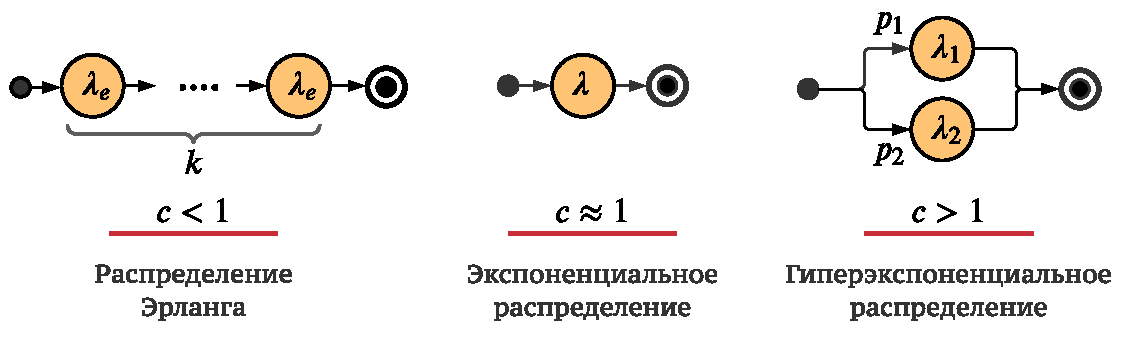
\includegraphics[width=0.80\textwidth]{chapter4/ch4_ph2.pdf}
  }
  \caption{PH-распределения для аппроксимации потоков по двум моментам}
  \label{fig:ch4_ph2}
\end{figure}

Если $c \approx 1$, то $\tilde{X} \sim Exp(\lambda)$. Матрицы MAP-потока $MAP(\tilde{D}_0, \tilde{D}_1)$ определяются с помощью выражения~\eqref{eq:ch4_map_ph_representation}.

Если $c > 1$, то $\tilde{X}$ -- гиперэкспоненциальное распределение с вероятностями $\overline{p} = (p_1, p_2)$ и интенсивностями $\overline{\lambda} = (\lambda_1, \lambda_2)$. Отметим, что интенсивности $\lambda_1, \lambda_2$ и вероятности $p_1$ и $p_2 = 1 - p_1$ определяются неоднозначно, так как ограничение на среднее и коэффициент вариации дают только два уравнения при трех неизвестных. Будем использовать следующее решение:
$$
\lambda_2 = \frac{1}{m_1} + 1,\quad \lambda_1 = \frac{m_1}{b \lambda_2 - m_1}, \quad p_1 = \frac{m_1^2}{b \lambda_2^2 - 2 m_1 \lambda_2 + 1},
$$
где $b = m_1^2(c^2 + 1) / 2$. Матрицы MAP-потока будут иметь вид:
$$
\tilde{D}_0 = \left(
    \begin{matrix}
        -\lambda_1 & 0\\
        0 & -\lambda_2
    \end{matrix}
    \right),\qquad
\tilde{D}_1 = \left(
    \begin{matrix}
        p_1 \lambda_1 & p_2 \lambda_1\\
        p_1 \lambda_2 & p_2 \lambda_2
    \end{matrix}
    \right).\qquad
$$

Наконец, если $c < 1$, то $\tilde{X}$ -- распределение Эрланга с числом состояний $k = \left[ 1 / c^2 \right]$ и параметром (интенсивностью каждого состояния) $\lambda_e = k / m_1$. Матрицы MAP-потока:
$$
\tilde{D}_0 = \left(
    \begin{matrix}
        -\lambda_e & \lambda_e & 0 & \cdots & 0\\
        0 & -\lambda_e & \lambda_e & \cdots & 0\\
        \vdots & \vdots & \vdots & \ddots & \vdots\\
        0 & 0 & 0 & \cdots &-\lambda_e
    \end{matrix}
    \right),\qquad
\tilde{D}_1 = \left(
    \begin{matrix}
        0 & 0 & \cdots & 0\\
        \vdots & \vdots & \ddots & \vdots\\
        0 & 0 & \cdots & 0\\
        \lambda_e & 0 & \cdots & 0
    \end{matrix}
    \right).\qquad
$$
Отметим, что коэффициент вариации $\tilde{c}$ может не совпадать в точности с исходным $c$ из-за округления.





%%% ~~~~~~~~~~~~~~~~
\subsection{Аппроксимация по трем моментам}\label{sec:ch4_approx_m3}
%%% ~~~~~~~~~~~~~~~~

Для большей точности результатов можно учитывать не только среднее значение $m_1$ и коэффициент вариации $c$ MAP-потока $X$, но и его коэффициент асимметрии $\gamma$. Существует ряд исследований, посвященных построению PH-распределений по трем и более моментам \cite{Osogami2006,Bobbio2005,Johnson1989,Telek2003,Horvath2013a,VandenBosch2000,Horvath2007,Schmickler1992}. Для упрощения задачи, поиск проводится не на всем классе PH-распределений, а на некотром его подмножестве. Например, в работах \cite{Bobbio2005,Telek2003} используются ациклические PH-распределения (APH), а в работе \cite{Johnson1989} используется распределение, представленное смесью двух распределений Эрланга с одинаковым числом фаз ($\text{ME}_\text{n}(2)$).

В общем случае PH-распределение можно найти для любого набора значений $m_1 > 0$, $c > 0$ и $\gamma > c - 1/c$, которыми может обладать какое-либо непрерывное положительное распределение \cite{Johnson1989}. Однако, порядок такого PH-распределения может быть очень большим. Например, в работе \cite{Aldous1987} было доказано, что при $c < 1$ самым малым порядком среди всех распределений с таким коэффициентом вариации  обладает распределение Эрланга. При этом порядок распределений Эрланга равен $1 / c^2$, то есть растет квадратично при приближении коэффициента вариации к нулю. Таким образом, если хочется получить PH-распределение с ограниченным числом фаз, то неизбежно приходится также ограничивать и область значений параметров $m_1, c, \gamma$ (особенно в области $c < 1$). Если же нужно иметь возможность получить PH-распределение для произвольных $m_1, c, \gamma$, то приходится смириться с неограниченным ростом сложности такого распределения.

\begin{figure}[h]
  \centerfloat{
    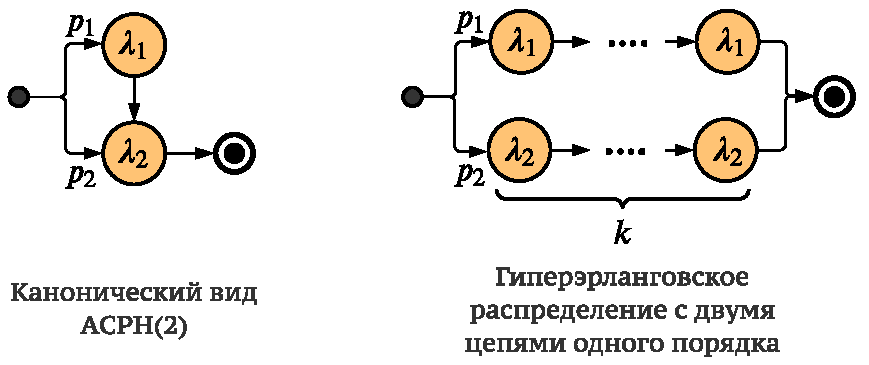
\includegraphics[width=0.6\textwidth]{chapter4/ch4_ph3.pdf}
  }
  \caption{Ациклическое PH-распределение с двумя состояниями ACPH(2) и гиперэрланговское распределение с двумя цепочками Эрланга одинакового порядка $\text{ME}_\text{n}(2)$, используемые при аппроксимации потоков по трем моментам.}
  \label{fig:ch4_ph3}
\end{figure}

В диссертационной работе будут использоваться два простых метода. Во-первых, попытаемся построить ациклическое PH-распределение второго порядка (ACPH(2)) в каноническом виде (см. рис.~\ref{fig:ch4_ph3}, левая схема) с помощью метода, описанного в работе Telek и Heindl \cite{Telek2003}. Если моменты не попадают в область существования ACPH(2) (см. рис.~\ref{fig:ch4_ph_feasible_regions}), то используем более универсальный метод, предолженный Johnson и Taafe \cite{Johnson1989}, с помощью которого PH-распределение ищется в виде смеси двух распределений Эрланга $ME_n(2)$ (см. рис.~\ref{fig:ch4_ph3}, правая схема). Опишем эти методы подробнее.

\begin{figure}[h]
  \centerfloat{
    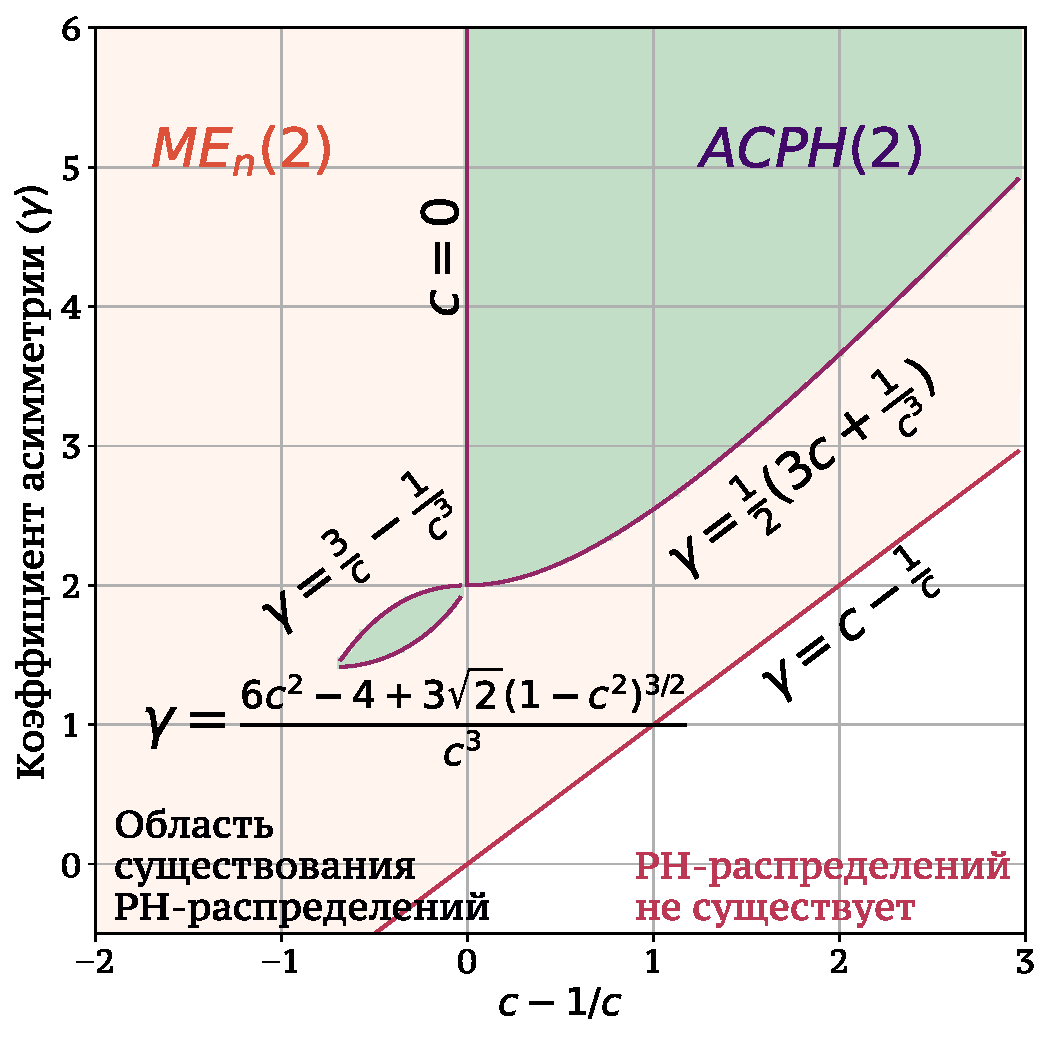
\includegraphics[width=0.5\textwidth]{chapter4/ch4_feasible_regions}
  }
  \caption{Области существования PH-распределений. Зеленым цветом показана область существования ACPH(2) \cite{Telek2003}, розовым -- произвольных PH-распределений, в частности $\text{ME}_\text{n}(2)$ \cite{Johnson1989}. Ниже линии $\gamma = c - 1/c$ PH-распределений не существует}
  \label{fig:ch4_ph_feasible_regions}
\end{figure}

Ациклические PH-распределения второго порядка ACPH(2) существуют в ограниченной области \cite{Telek2003}. Границы области можно выразить через коэффициенты асимметрии $\gamma$ и вариации $c$:

\begin{equation}
    \label{eq:ch4_acph2_existance}
    \begin{matrix}
        \frac{6c^2 - 4 + 3\sqrt{2}(1 - c^2)^{\frac{3}{2}}}{c^3} \leqslant \gamma \leqslant \frac{3c^2 - 1}{c^3}, & \frac{1}{\sqrt{2}} \leqslant c \leqslant 1\\
        \frac{1}{2}(3c + \frac{1}{c^3}) \leqslant \gamma, & c > 1
    \end{matrix}
\end{equation}
При $c < 1/\sqrt{2}$ распределений ACPH(2) не существует. Область существования показана на рис.~\ref{fig:ch4_ph_feasible_regions}.

Распределение ACPH(2) определяется тремя параметрами $\lambda_1$, $\lambda_2$ и $p_1$ (вероятность $p_2 = 1 - p_1$), см. рис.~\ref{fig:ch4_ph3}. Их можно вычислить следующим  образом:

\begin{equation}
    \label{eq:ch4_acph2_params}
    p = \frac{-B + 6 m_1 D + \sqrt{A}}{B + \sqrt{A}}, \quad
    \lambda_{1} = \frac{B - \sqrt{A}}{C}, \quad
    \lambda_{2} = \frac{B + \sqrt{A}}{C}
\end{equation}
где $D = 2m_1^2 - m_2$, $C = 3 m_2^2 - 2 m_1 m_3$, $B = 3 m_1 m_2 - m_3$ и $A = B^2 - 6 C D$. Здесь $m_i = \mathbb{E}X^i$ -- $i$-й момент случайной величины. Моменты $m_2$ и $m_3$ можно выразить через коэффициент вариации $c$ и асимметрии $\gamma$ как $m_2 = m_1 c^2 + m_1^2$ и $m_3 = m_1^3 (c^3 \gamma + 3 c^2 + 1)$. Матрица $S$ и вектор начального распределения $\overline{\tau}$ для ACPH(2) будут иметь следующий вид:

\begin{equation}
    \label{eq:ch4_acph2_ph_tau}
    S = \left(\begin{matrix}
        -\lambda_1 & \lambda_1 \\
        0 & -\lambda_2
    \end{matrix}\right),
    \qquad
    \overline{\tau} = \left(\begin{matrix}
        p_1 & 1 - p_1
    \end{matrix}\right).
\end{equation}

Если коэффициенты $c$ и $\gamma$ аппроксимируемого потока не удовлетворяют ограничениями \eqref{eq:ch4_acph2_existance}, то будем искать PH-распределение в классе $\text{ME}_\text{n}(2)$. В отличие от узкого класса ACPH(2), распределения $\text{ME}_\text{n}(2)$ существуют для любого значения $\gamma > c - 1/c$, то есть их область существования совпадает с областью существования произвольных PH-распределений \cite{Johnson1989}. Соотношение между областями существования ACPH(2) и $\text{ME}_\text{n}(2)$ показано на рис.~\ref{fig:ch4_ph_feasible_regions}. Распределения $\text{ME}_\text{n}(2)$ представляют собой смесь двух распределений Эрланга одинакового порядка $n$ с вероятностями $p_1$ и $p_2 = 1 - p_1$. Распределения Эрланга имеют параметры $\lambda_1$ и $\lambda_2$ (см. рис.~\ref{fig:ch4_ph3}). Минимальный порядок $n^*$ распределений Эрланга в $\text{ME}_\text{n}(2)$ для заданных значений $c$ и $\gamma$ определяется согласно утверждению 4 из работы \cite{Johnson1989}:

\begin{equation}
    \label{eq:ch4_men2_min_n}
    n^* = \lceil \max \lbrace
            \frac{1}{c^2}, \;
            \frac{-\gamma + 1/c^3 + 1/c + 2c}{\gamma - (c - 1/c)}
        \rbrace \rceil
\end{equation}

После выбора $n \geqslant n^*$ можно вычислить параметры $\lambda_1$, $\lambda_2$ и $p_1$. Способ вычисления описан в теореме 3 \cite{Johnson1989}:

\begin{equation}
    \label{eq:ch4_men2_params}
    \lambda_i^{-1} = \frac{-B \pm \sqrt{B^2 - 4 A C}}{2 A}, \qquad
    p_1 = \frac{m_1/n - \lambda_2^{-1}}{\lambda_1^{-1} - \lambda_2^{-1}},
\end{equation}
где
\begin{equation}
    \label{eq:ch4_men2_params_aux}
    \begin{aligned}
        A &= n(n+2) m_1 y\\
        B &= -\left( nx + \frac{n(n+2)}{n+1}y^2 + (n+2) m_1^2 y \right)\\
        C &= m_1 x\\
        x &= m_1 m_3 - \frac{n+2}{n+1} m_2^2\\
        y &= m_2 - \frac{n+1}{n} m_1^2
    \end{aligned}
\end{equation}
Матрица $S$ и вектор начального распределения $\overline{\tau}$ для PH-распределения из класса $\text{ME}_\text{n}(2)$ будут иметь вид:

\begin{equation}
    \label{eq:ch4_men2_ph_tau}
    \begin{aligned}
        S &= \left(\begin{blockarray}{cccc|cccc}
            -\lambda_1 & \lambda_1 & & & & & & \\
             & -\lambda_1 & \lambda_1 & & & & & \\
             & & \ddots & & & \text{\Huge0} & & \\
            & & & -\lambda_1 & & & & \\
            \cline{1-8}
             & & & & -\lambda_2 & \lambda_2 & & \\
             & & & & & -\lambda_2 & \lambda_2 & \\
            & \text{\Huge0} & & & & & \ddots &\\
            & & & & & & & -\lambda_2
        \end{blockarray}\right)\\
        \overline{\tau} &= (\begin{matrix}
        p_1 & 0 & \dots & 0 & | & 1 - p_1 & 0 & \dots & 0
        \end{matrix}).
    \end{aligned}
\end{equation}

В работе Johnson и Taafe~\cite{Johnson1989} приведен подробный анализ класса $\text{ME}_\text{n}(2)$, а также есть рекомендации, что делать, если $\lambda_1 / \lambda_2 \gg 1$, $\lambda_1 / \lambda_2 \ll 1$ или $p_i \approx 1$. Например, небольшое увеличение $n$ может сблизить $\lambda_1$ и $\lambda_2$. Хотя некоторые из рекомендаций были реализованы, в диссертационной работе будем использовать простейшую форму построения $\text{ME}_\text{n}(2)$, так как хотелось бы избежать как дополнительного роста размерности, так и существенных отклонений в коэффициентах вариации и асимметрии.

Объединяя все изложенное выше, будем искать PH-распределение по трем моментам следующим образом.

\begin{enumerate}
    \item Если $c \approx 1$, $\gamma \approx 2$, то строим экспоненциальное распределение с $\lambda = 1/m_1$. Матрицы искомого MAP-потока будут иметь вид~\eqref{eq:ch4_map_from_exp}.
    \item Если коэффициенты $c$ и $\gamma$ удовлетворяют условиям $c > 1/\sqrt{2}$ и~\eqref{eq:ch4_acph2_existance}, то строим распределение ACPH(2):
    \begin{enumerate}
        \item Рассчитываем параметры $\lambda_1$, $\lambda_2$ и $p_1$ с помощью~\eqref{eq:ch4_acph2_params}.
        \item Строим матрицу $S$ и вектор $\overline{\tau}$ с помощью~\eqref{eq:ch4_acph2_ph_tau}.
    \end{enumerate}
    \item Если для заданных $c$ и $\gamma$ распределения ACPH(2) не существует, то строим распределение $\text{ME}_\text{n}(2)$:
    \begin{enumerate}
        \item Рассчитываем параметры $\lambda_1$, $\lambda_2$ и $p_1$ с помощью~\eqref{eq:ch4_men2_params} и~\eqref{eq:ch4_men2_params_aux}.
        \item Строим матрицу $S$ и вектор $\overline{\tau}$ с помощью~\eqref{eq:ch4_men2_ph_tau}.
    \end{enumerate}
    \item Для найденного распределения $PH(S, \overline{\tau})$ строим матрицы MAP-потока $D_0$ и $D_1$ с помощью выражения \eqref{eq:ch4_map_ph_representation}.
\end{enumerate}

В завершение отметим, что вместо алгоритмов из работ~\cite{Telek2003} и~\cite{Johnson1989} можно использовать любые другие алгоритмы, позволяющие построить PH-распределение по трем моментам.



%%% ~~~~~~~~~~~~~~~~
\subsubsection{Аппроксимация по трем моментам и автокорреляции}\label{sec:ch4_approx_m3_lag1}
%%% ~~~~~~~~~~~~~~~~

Последний вариант аппроксимаций, который будет рассматриваться в диссертационном исследовании, это аппроксимация MAP-потока другим MAP-потоком с теми же первыми тремя моментами и коэффициентом автокорреляции с лагом 1, то есть корреляцией между соседними интервалами между возникновением событий в MAP-потоке. Как и ранее, ключевая идея здесь заключается в том, чтобы понизить размерность MAP-потока: если учитывать только ограниченный набор характеристик, то есть шанс получить MAP-поток меньшего размера.

Для поиска аппроксимирующего MAP-потока будем пользоваться методом, предложенным Horvath и соавторами в работе~\cite{Horvath2005}. Согласно этому подходу, матрицы $D_0$ и $D_1$ ищутся независимо по значениям моментов и коэффициентам автокорреляции. Метод основан на том, что стационарное распределение MAP-потока, определяющее его моменты, есть $PH(D_0,\, \overline{\alpha})$, где $\overline{\alpha}$ "--- стационарное распределение вложенной по моментам появления событий цепи с матрицей $P = (-D_0)^{-1} D_1$. Поэтому можно найти матрицу $D_0$ и вектор $\overline{\alpha}$, используя любой из ранее описанных методов для поиска PH-распределений, а информацию о значениях коэффициентов автокорреляции использовать для поиска матрицы $D_1$.

В общем случае поиск элементов матрицы $D_1 \in \mathbb{R}^{W \times W}$ по известным коэффициентам автокорреляции с лагами $i=1, 2, \dots, L$ можно сформулировать как задачу оптимизации:

\begin{equation}
    \label{eq:ch4_map_lag_opt_criterion}
    D_1 = \argmin \limits \sum\limits_{i=1}^L w_i \left(\frac{\lambda \overline{\pi} (-D_0)^{-k} D_1^k (-D_0)^{-1} \overline{\mathbf{1}} - 1}{2 \overline{\pi} (-D_0)^{-1} \overline{\mathbf{1}} - 1} - \rho_i \right)^2
\end{equation}
с ограничениями
\begin{equation}
    \label{eq:ch4_map_lag_opt_constraints}
    \begin{aligned}
        &D_1 \overline{1} = -D_0 \overline{1}\\
        &\overline{\alpha} (-D_0)^{-1} D_1 = \overline{\alpha}\\
        &\{D_1\}_{ij} \geqslant 0,\quad i, j = \overline{1, W}.
    \end{aligned}
\end{equation}
Здесь $w_i$, $i = 1, 2, \dots, L$ "--- веса, с помощью которых можно регулировать важность приближения того или иного момента. Отметим, что ограничения \eqref{eq:ch4_map_lag_opt_constraints} линейны относительно элементов матрицы $D_1$.
Кроме ограничений \eqref{eq:ch4_map_lag_opt_constraints} также нужно убедиться, что управляющая цепь с генератором $D = D_0 + D_1$ неприводима.

Ограничением применения метода является то, что диапазон возможных значений $\rho_i$ определяется выбором стационарного PH-распределения. В общем случае, для заданных $m_1$, $c$ и $\gamma$ PH-распределение определяется неоднозначно, его вид зависит от используемых методов. Возможна ситуация, когда PH-распределение найти удалось, а матрицу $D_1$ для MAP-потока с заданными коэффициентами корреляции $\rho_i$ "--- нет, хотя MAP-поток с искомыми параметрами существует.

Пусть $L = 1$. Функция
$$
\rho(D_1) = \frac{\lambda \overline{\pi} (-D_0)^{-1} D_1 (-D_0)^{-1} \overline{\mathbf{1}} - 1}{2 \overline{\pi} (-D_0)^{-1} \overline{\mathbf{1}} - 1},
$$
принимающая значение коэффициента корреляции с лагом 1, представляет собой линейную комбинацию элементов матрицы $D_1$. Значит, для нахождения минимального $\underline{\rho_1}$ и максимально $\hat{\rho}_1$ значения $\rho_1$ при заданной матрице $D_0$ можно использовать симплекс-метод:

\begin{equation}
    \label{eq:ch4_approx_map_rho_boundaries}
    \begin{aligned}
        \hat{\rho}_1 &= \max \rho(D_1)\\
        \underline{\rho_1} &= \min \rho(D_1)
    \end{aligned}
\end{equation}
при ограничениях \eqref{eq:ch4_map_lag_opt_constraints}. Пользуясь выпуклостью задачи линейного программирования, если заданное значение $\rho_1 \in [\underline{\rho_1}, \hat{\rho}_1]$, то матрицу $D_1$ можно найти, решая систему линейных алгебраических уравнений относительно элементов матрицы $D_1$:

\begin{equation}
    \label{eq:ch4_map_lag_opt_ales}
    \begin{cases}
        D_1 \overline{1} &= -D_0 \overline{1}\\
        \overline{\alpha} (-D_0)^{-1} D_1 &= \overline{\alpha}\\
        \frac{\lambda \overline{\pi} (-D_0)^{-1} D_1 (-D_0)^{-1} \overline{\mathbf{1}} - 1}{2 \overline{\pi} (-D_0)^{-1} \overline{\mathbf{1}} - 1} &= \rho_1
    \end{cases}
\end{equation}
Отметим, что если порядок искомого MAP-потока $W > 1$, то у системы будет бесконечное множество решений. Если $\rho_1 > \hat{\rho}$ или $\rho_1 < \underline{\rho_1}$, то будем брать ту матрицу $D_1$, которая соответствует найденному ранее экстремуму.

На практике иногда возникает ситуация, когда результатом решения проблемы \eqref{eq:ch4_map_lag_opt_criterion} является такая матрица $D_1$, что цепь Маркова с генератором $D = D_0 + D_1$ не является неприводимой. Для быстрой проверки неприводимости удобно использовать алгоритм Тарьяна \cite{tarjan72} для поиска сильно-связных компонент графа. Сильно-связная компонента "--- это такой набор вершин графа, в котором из каждой вершины можно попасть в любую другую вершину. Если цепь состоит из единственной сильно-связной компоненты, то она является неприводимой. Для повышения качества результатов, при построении графа будем игнорировать переходы между состояниями цепи, вероятности которых крайне малы. Чтобы подчеркнуть важность проверки на неприводимость отметим, что в ходе численных экспериментов, которые будут обсуждаться далее, около 16\% всех построенных MAP-потоков имели не неприводимые цепи.

Если полученная цепь $D = D_0 + D_1$ не является неприводимой, то есть несколько возможных действий. Во-первых, так как проблемы \eqref{eq:ch4_map_lag_opt_criterion} и \eqref{eq:ch4_map_lag_opt_ales} могут иметь множество решений, можно попытаться найти другую матрицу $D_1$ с той же матрицей $D_0$ и вектором $\overline{\alpha}$. Во-вторых, можно попытаться найти другое распределение $PH(D_0, \overline{\alpha})$ с теми же моментами. Для этого можно использовать другой метод, или ослабить требования точности на третий и/или второй моменты. В-третьих, можно найти другую матрицу $D_1$, для которой $\rho(D_1)$ будет близко, но не равно в точности значению $\rho_1$. В нашей работе мы используем третий подход.

В завершение отметим, что существуют и другие подходы к построению MAP-потоков по моментам и коэффициентам автокорреляции, например~\cite{TelekHorvath2007,Bodrog2010}. Кроме того, MAP-потоки можно строить по выборке (ее можно получить из аппроксимируемого потока), используя EM-процедуру \cite{Horvath2013,Ephraim2009,Buchholz2003}.


%%% ~~~~~~~~~~~~~~~~
\subsection{Сложность и применимость метода}\label{sec:ch4_approx_complexity}
%%% ~~~~~~~~~~~~~~~~

Хотя метод понижения размерности позволяет находить оценки характеристик сетей массового обслуживания с произвольно большим числом узлов, он, как и метод Монте-Карло, не может обеспечить очень быстрый расчет. Проблема состоит в том, что размерности потоков нельзя сделать сколь угодно низкими. Хорошо известно \cite{Aldous1987}, что если коэффициент вариации $c$ искомого распределения меньше единицы, то самое малое число состояний $K = \lceil 1 / c^2 \rceil $ будет у распределения Эрланга. Таким образом, неограниченного роста размерности невозможно избежать даже тогда, когда для приближения используется всего два первых момента. Пусть $\hat{c} = \min\{c_1, c_2, \dots, c_{N-1}\}$ "--- минимальный коэффициент вариации среди всех выходных потоков кроме последнего узла, который здесь не играет роли, и $\hat{W} = \max\{\lceil 1 / \hat{c}^2 \rceil, W\}$. Тогда сложность алгоритма можно оценить как $\mathcal{O}(N (\hat{W}MV)^3 )$. Конечно, это гораздо лучше экспоненциального роста сложности точного алгоритма, но все равно очень много. Еще стоит отметить, что хотя порядок PH-распределений слабее зависит от коэффициента асимметрии, чем от коэффициента вариации (см., например, \cite{Johnson1989}), для точного совпадения третьего момента и коэффициента корреляции также может потребоваться увеличить размерность. Наконец, поиск матрицы $D_1$ даже по коэффициенту корреляции с лагом один требует в общем случае решать задачу оптимизации, и это приходится делать для каждого выходного потока.




%%%%%%%%%%%%%%%%%%%%%%%%%%%%%%%%%%%%%%%%%%%%%%%%%%%%%%%%%%%%%%%%%%%%%%%%%%%%%%%%
\section{Моделирование задержки в канале}\label{sec:ch4_channel}
%%%%%%%%%%%%%%%%%%%%%%%%%%%%%%%%%%%%%%%%%%%%%%%%%%%%%%%%%%%%%%%%%%%%%%%%%%%%%%%%

В диссертационной работе предметом исследования является многошаговая беспроводная сеть сбора данных с камер или RFID-считывателей, работающая под управлением протокола IEEE 802.11 и передающая трафик в одном направлении. Будем считать, что все станции этой сети работают в одном канале, антенны у всех станций имеют круговую диаграмму, и станции расположены таким образом, что передачу любой станции могут получить только ее непосредственные соседи (см. рис.~\ref{fig:ch4_network_collisions}). В такой сети коллизия на станции $S_i$ возникнет при одновременной передаче ее соседей, то есть когда станция $S_{i-1}$ будет вести передачу станции $S_i$, а станция $S_{i+1}$ "--- станции $S_{i+2}$: из-за круговой диаграммы и использования общего канала, последнюю передачу также получит станция $S_i$.

\begin{figure}[h]
  \centerfloat{
    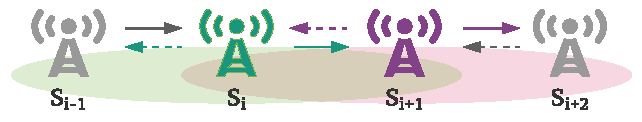
\includegraphics[width=0.5\textwidth]{chapter4/ch4_network_collisions}
  }
  \caption{Области видимости станций многошаговой беспроводной сети}
  \label{fig:ch4_network_collisions}
\end{figure}

Для моделирования длительности передачи пакетов в беспроводном канале с помощью PH-распределений нужно знать моменты этого распределения или иметь выборку длительностей. В диссертационном исследовании будем пользоваться методом восстановления PH-распределения по трем моментам, описанном в разделе~\ref{sec:ch4_approx_m3}, основанном на работах Johnson и Taafe~\cite{Johnson1989} и Telek и Heindl~\cite{Telek2003}.

Для получения оценок моментов распределения длительностей передачи пакетов можно использовать аналитические или имитационные модели каналов. Например, в работах \cite{QS_ICAAPSP2020,QS_ITMM2019} время передачи моделировалось с помощью полумарковского процесса для насыщенного режима, а также использовались простые имитационные модели каналов CSMA/CA для ненасыщенного режима. Если в качестве модели канала используется полумарковский процесс, то через вычисление функции генерации моментов можно получить значения математического ожидания и дисперсии для построенного этого процесса (см., например, работу Sakurai~\cite{Sakurai2007}). В результатах, представленных в диссертационном исследовании, использовалась более точная имитационная модель канала IEEE 802.11 из системы моделирования NS-3.

Длительность передачи в беспроводном канале определяется не только настройками приемников и передатчиков, но и вероятностью коллизий, которая зависит от числа конкурирующих станций. В исследуемой многошаговой сети станции работают в одном канале, поэтому вероятность коллизий зависит от положения станции внутри сети. Таким образом, для получения достаточно точных оценок нужно использовать разные PH-распределения на разных приборах.

\begin{figure}[h]
  \centerfloat{
    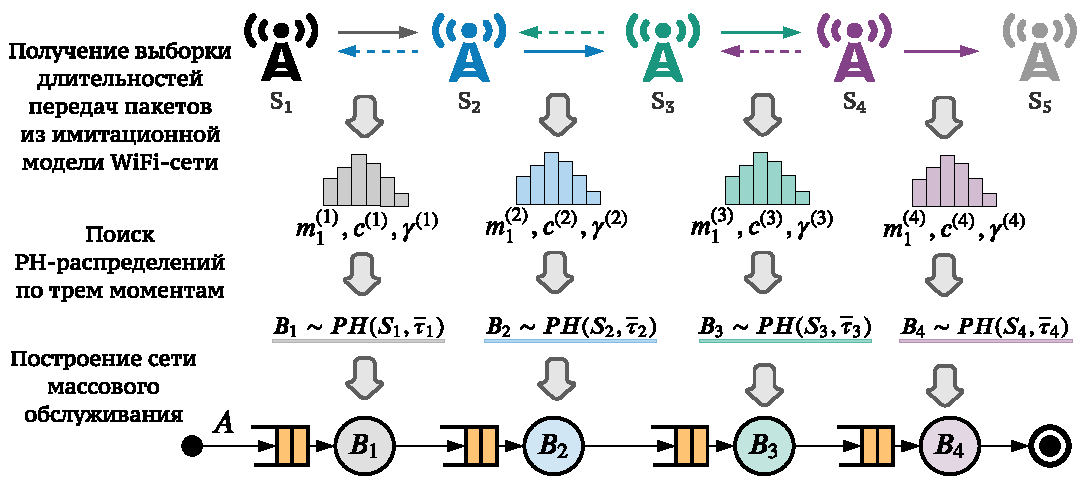
\includegraphics[width=0.85\textwidth]{chapter4/ch4_channel_model_schema}
  }
  \caption{Схема моделирования каналов беспроводной сети}
  \label{fig:ch4_channel_model_schema}
\end{figure}

Рассмотрим сеть, состоящую из пяти станций (см. рис.~\ref{fig:ch4_channel_model_schema}). Возможны четыре различных случая:

\begin{enumerate}
  \item Канал $S_1 \rightarrow S_2$: канал занят, если станция $S_2$ ведет передачу; возможна коллизия с передачами станции $S_3$.
  \item Канал $S_2 \rightarrow S_3$: канал занят, если станции $S_1$ или $S_3$ ведут передачу; возможна коллизия с передачами станции $S_4$.
  \item Канал $S_3 \rightarrow S_4$: канал занят, если станция $S_2$ или $S_4$ ведут передачу; станция $S_5$ "--- конечная, далее не передает, поэтому коллизий нет.
  \item Канал $S_4 \rightarrow S_5$: канал занят, если станция $S_3$ ведет передачу; коллизий нет.
\end{enumerate}

Для каждого из этих каналов строится отдельное PH-распределение $B_1$, $B_2$, $B_3$ и $B_4$ (номер распределения совпадает с номером станции-отправителя). Если сеть содержит меньше станций, то и распределений потребуется меньше.

\begin{figure}[h]
  \centerfloat{
    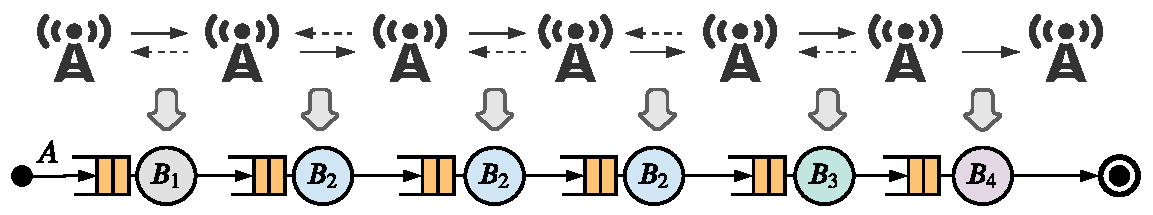
\includegraphics[width=0.8\textwidth]{chapter4/ch4_network_model_schema}
  }
  \caption{Схема моделирования беспроводной сети с произвольным числом станций}
  \label{fig:ch4_network_model_schema}
\end{figure}

Если добавятся промежуточные станции, то новые каналы будут испытывать нагрузку, аналогичную каналу $S_2 \rightarrow S_3$, поэтому сеть можно моделировать с помощью тех же распределений $B_1$, $B_2$, $B_3$ и $B_4$ (см. рис.~\ref{fig:ch4_network_model_schema}).



%%%%%%%%%%%%%%%%%%%%%%%%%%%%%%%%%%%%%%%%%%%%%%%%%%%%%%%%%%%%%%%%%%%%%%%%%%%%%%%%
\section{Численное исследование эффективности метода аппроксимации потоков}
%%%%%%%%%%%%%%%%%%%%%%%%%%%%%%%%%%%%%%%%%%%%%%%%%%%%%%%%%%%%%%%%%%%%%%%%%%%%%%%%

Для исследования эффективности метода вычисления оценок характеристик тандемной сети массового обслуживания, был проведен ряд численных экспериментов на случайном наборе данных. Входящий набор данных включал \hl{2500} сетей со случайными значениями среднего времени обслуживания, коэффициентов вариации и асимметрии интервалов между пакетами и времен обслуживания, коэффициента автокорреляции входящего MAP-потока с единичным лагом, случайными емкостями очередей и случайным числом станций в сети. На всех наборах были найдены решения методом Монте-Карло и всеми методами аппроксимации потоков, описанных в разделе~\ref{sec:ch4_approx}. На тех входных данных, на которых это было возможно, было найдено точное решение.

Сначала рассмотрим, как был сгенерирован набор входных данных для исследования методов аппроксимации выходящих потоков. Затем приведем результаты измерения ошибок, возникающих при использовании этих методов. В завершение покажем, как меняется точность метода Монте-Карло при увеличении числа сгенерированных пакетов.


%%% ~~~~~~~~~~~~~~~~
\subsection{Построение набора данных для исследования}
%%% ~~~~~~~~~~~~~~~~

Для проведения численных экспериментов были сгенерированы \hl{2000} входных параметров со случайными средними временами обслуживания, коэффициентами вариации интервалов между пакетами $c_a$ и обслуживания $c_s$, коэффициентами асимметрии поступления $\gamma_a$ и обслуживания $\gamma_s$, коэффициентами автокорреляции входящего потока $\rho_l$, числом узлов в сети и емкостью очередей. Интенсивность (и, соответственно, средний интервал) входящего потока во всех случаях полагалась равной единице, поэтому коэффициент загрузки первого узла был равен $m_s / m_a = m_s$. Границы значений параметров для стандартного генератора показаны в табл.~\ref{tab:ch4_results_approx_input_range}. Отметим, что так как емкости очередей в системе ограничены, и переполняющие очередь пакеты теряются, исследовать системы с коэффициентом загрузки $m_s / m_a > 1$ корректно. Для построения PH-распределений времени обслуживания по выбранным случайным параметрам $m_s, c_s, \gamma_s$ использовались методы, описанные в разделах \ref{sec:ch4_approx_m1}, \ref{sec:ch4_approx_m2} и \ref{sec:ch4_approx_m3}, а для построения MAP-потоков по $m_a \equiv 1, c_a, \gamma_a, \rho_1$ "--- метод из раздела \ref{sec:ch4_approx_m3_lag1}.

\begin{table}[h]
  \centering
  \caption{\label{tab:ch4_results_approx_input_range} Граничные значения параметров для исследования методов аппроксимации потоков.}
  \begin{tabular}{|c|cc|cc|}
    \hline
    \multirow{2}{*}{Параметр}
      &\multicolumn{2}{c|}{Стандартный генератор}&\multicolumn{2}{c|}{Простые распределения}\\
                    &Мин.   &Макс.    &Мин.   &Макс.\\
      \hline
      $m_s$           &0,1       &1,5        &0,1        &1,5\\
      $c_s$,$c_a$     &0,5       &4,0        &0,5        &4,0\\
      $\gamma_{a,s}$  &$c_{a,s} - 1/c_{a,s}$ &6.0    &\multicolumn{2}{c|}{Не используется}\\
    $\rho_1$        &\multicolumn{4}{c|}{Границы рассчитываются как решение задачи
      \eqref{eq:ch4_approx_map_rho_boundaries}}\\
    Размер сети $N$ &1          &10        &3           &10\\
    Емкость очереди $M$ &0      &10        &0           &3\\
    \hline
  \end{tabular}
\end{table}


Сложность итерационного алгоритма для точного расчета характеристик сети растет экспоненциально с ростом числа узлов. Для получения точного решения требовалось, чтобы порядок матриц выходящего потока с последнего узла был достаточно мал. В противном случае матрицы могут просто не поместиться в оперативной памяти или потребуют слишком много времени для выполнения операции обращения и получения решения системы линейных уравнений. Следуя этой логике, для получения точного решения использовались только те входные данные, на которых матрица потока обслуженных заявок на последнем узле имеет порядок не выше 8000. После такого отсева оставалось слишком мало входных наборов, поэтому дополнительно были сгенерированы 1000 наборов входных параметров, в которых использовались более простые распределения и меньшие очереди: PH-распределение времени обслуживаня и стационарное PH-распределение MAP-потоков строились по первым двум моментам (см. раздел \ref{sec:ch4_approx_m2}), а не трем, длина очереди выбиралась из меньшего диапазона, а число узлов ограничивалось снизу, см. табл.~\ref{tab:ch4_results_approx_input_range}.

\begin{figure}[h]
  \centerfloat{
    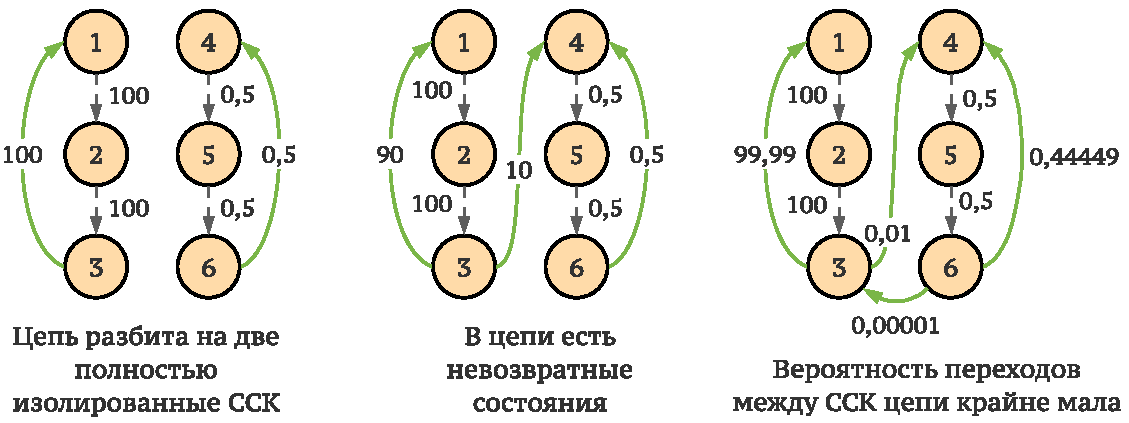
\includegraphics[width=0.8\textwidth]{chapter4/ch4_results_bad_maps.pdf}
  }
  \caption{Примеры отсеиваемых MAP-потоков. На стрелках показана интенсивность переходов. Сплошные линии "--- переходы матрицы $D_1$, пунктирные "--- $D_0$}.\label{fig:ch4_results_bad_maps}
\end{figure}

В итоге были получены \hl{3000} входных наборов. Как было отмечено в разделе \ref{sec:ch4_approx_m3_lag1}, иногда построенные MAP-потоки не были неприводимыми. В некоторых случаях пространство состояний распадалось на две сильно связные компоненты, соответствующие цепочкам Эрланга. Примеры <<плохих>> MAP-потоков показаны на рис.~\ref{fig:ch4_results_bad_maps}. Если бы такие потоки использовались при расчете методом Монте-Карло, были бы получены некорректные результаты. Например, запуская имитационную модель (реализацию метода Монте-Карло) два раза, и выбирая в качестве начального состояния MAP-потока состояние сначала из первой, а затем из второй компоненты, по сути рассматривались бы два разных потока, так как попасть из состояний одной компоненты в другую невозможно, и, таким образом, были бы получены разные результаты. Для того, чтобы быстро отсеить <<плохие>> потоки, был использован алгоритм Тарьяна поиска сильно-связных компонентов в графе~\cite{tarjan72}. Множество вершин такого графа совпадает с множеством состояний цепи, а дуга между состояниями $i$ и $j$ в графе есть только в том случае, если вероятность перехода во вложенной цепи $\mathbb{P}\{X_{n+1} = j | X_n = i\} > 10^{-3}$. Нижняя граница нужна, чтобы отсеить случаи, когда переходы между компонентами есть, но крайне маловероятны: такие переходы срабатывают редко, а переход по ним может существенно изменить оценки характеристик, поэтому для получения устойчивых результатов нужно моделировать огромное число событий.

\begin{figure}[h]
  \centerfloat{
    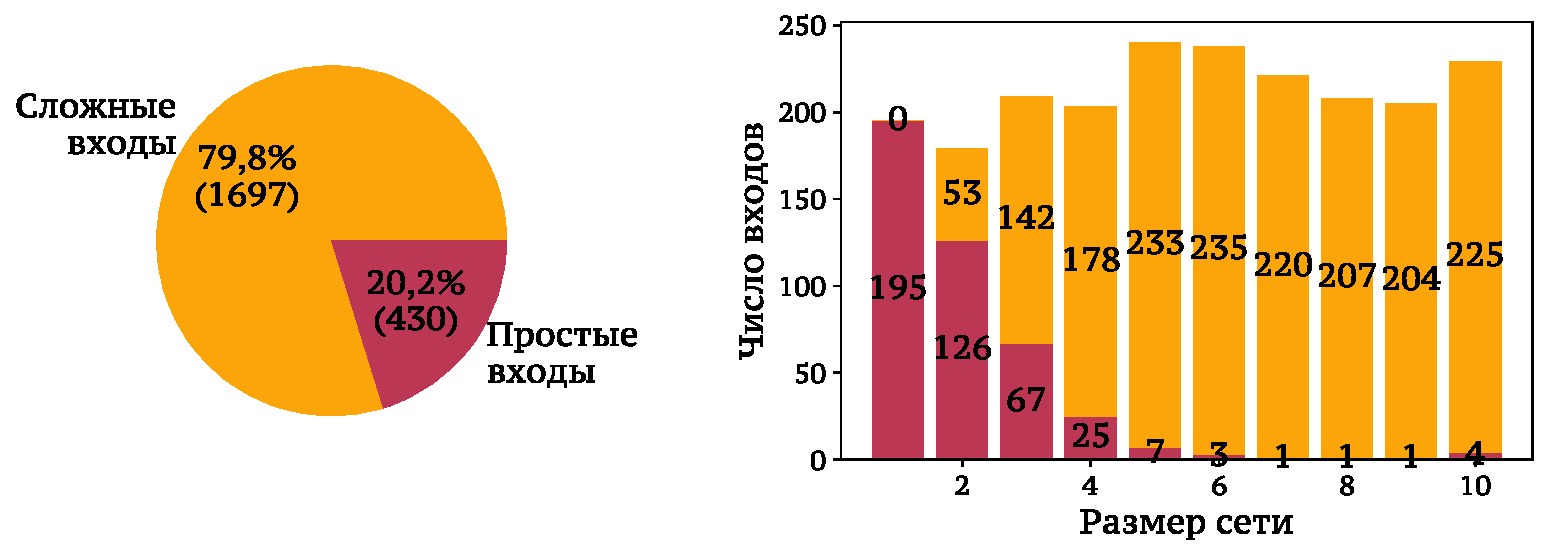
\includegraphics[width=0.8\textwidth]{chapter4/ch4_complexity_split}
  }
  \caption{Разбиение наборов входных данных на простые и сложные}\label{fig:ch4_complexity_split}
\end{figure}

В результате отсеивания было удалено \hl{579} входных наборов, то есть \hl{19,3\%} данных. Оставшиеся наборы были поделены на <<простые>> и <<сложные>>: к простым наборам были отнесены те, для которых порядок выходящего потока, равный $\hat{W}_N = W(V(M+2))^N$, не превосходил 8000, а все остальные "--- к сложным. Ожидаемо, большинство простых наборов соответствовали сетям малого размера, см. рис.~\ref{fig:ch4_complexity_split}. Так как для больших сетей простых наборов оказалось слишком мало, в дальнейшем точное решение искалось только для тех простых наборов, в которых длина сети не превышала 5.

\begin{figure}[h]
  \centerfloat{
    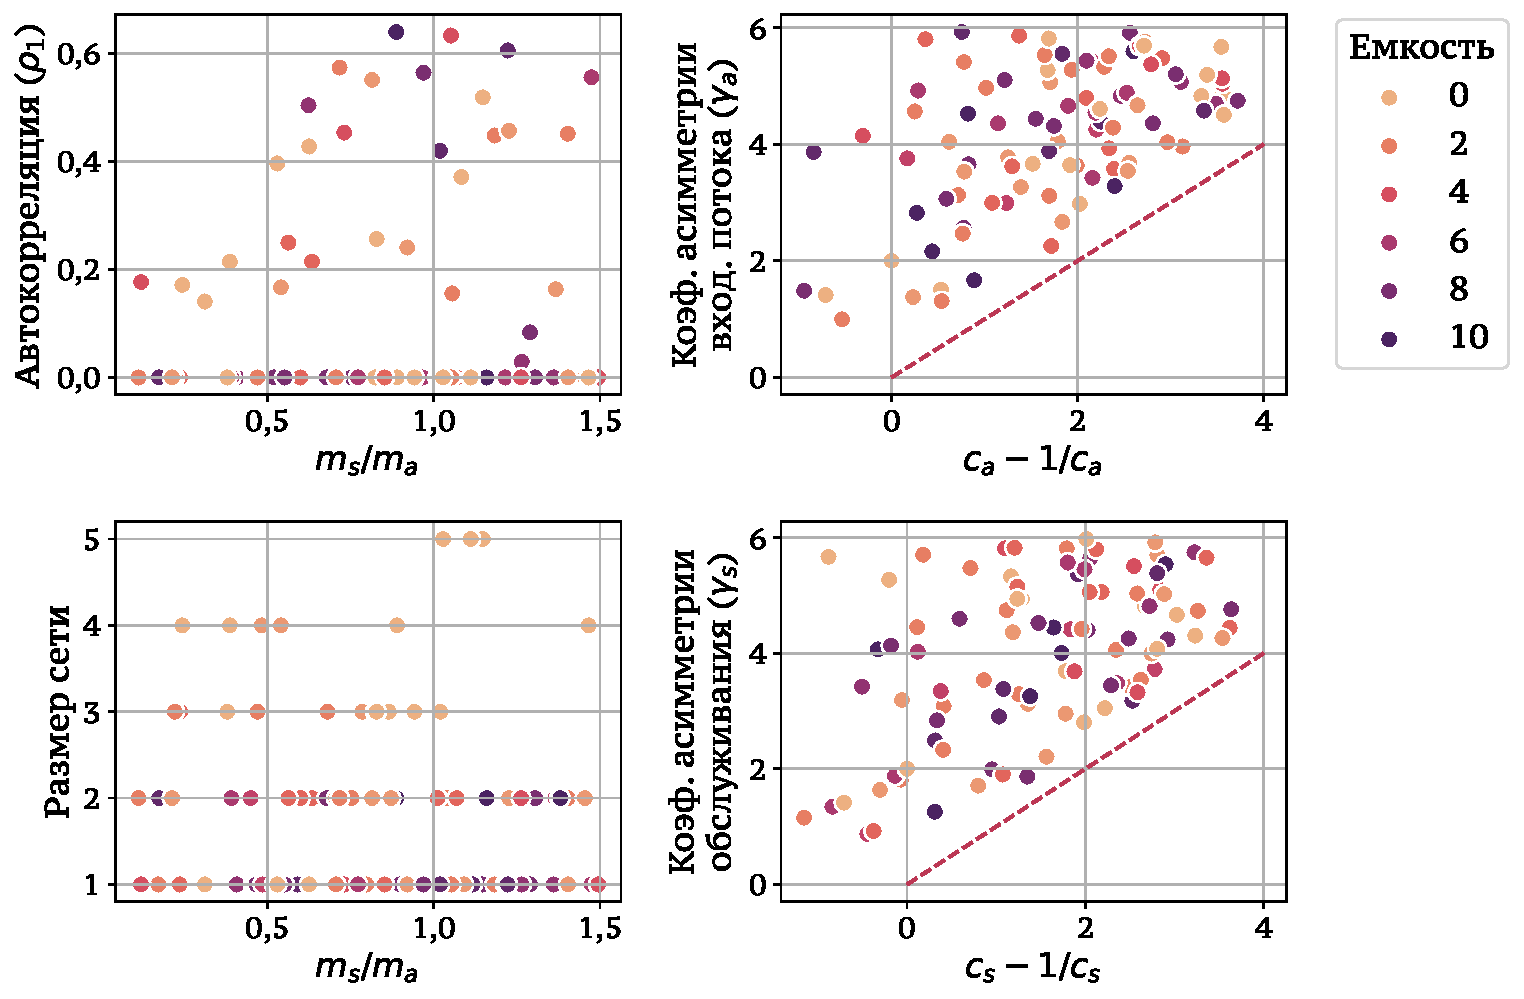
\includegraphics[width=0.8\textwidth]{chapter4/ch4_input_scatter}
  }
  \caption{Диаграммы разброса для различных сочетаний параметров в наборах простых входных данных. Размеры кругов соответствуют емкостям очередей}\label{fig:ch4_input_scatter}
\end{figure}

На рис.~\ref{fig:ch4_input_scatter} показаны диаграммы разброса различных параметров в наборах простых входных данных. Можно обратить внимание на три особенности. Во-первых, наборы распределены практически равномерно относительно коэффициента загрузки $m_s / m_a$. Во-вторых, у большей части наборов коэффициенты вариации $c_a$ и $c_s$ больше единицы. Это можно объяснить тем, что при $c < 1$ размерность PH-распределений не меньше, чем $\lfloor 1/c^2 \rfloor$, поэтому и $\hat{W}_N$ оказывается в среднем больше, чем для распределений с $c \geqslant 1$. В-третих, подавляющее большинство MAP-потоков имеют коэффициент корреляции $\rho_1 \geqslant 0$, причем у значительной части $\rho_1 \approx 0$. Это можно объяснить тем, что для тех матриц $D_0$, которые строиись с помощью методов, описанных в разделах \ref{sec:ch4_approx_m2} и \ref{sec:ch4_approx_m3}, нижняя граница $\rho_1 \approx 0$, а верхняя меняется от 0 до $0,8$. Отметим, что среди наборов достаточно таких, у которых автокорреляция $\rho_1 > 0$.



%%% ~~~~~~~~~~~~~~~~
\subsection{Использование методов аппроксимации выходящего потока}
%%% ~~~~~~~~~~~~~~~~

С помощью алгоритма, приведенного в разделе~\ref{sec:ch4_queue_net_precise}, были найдены точные решения для всех простых входных данных, для которых порядок выходного MAP-потока с последнего узла сети не превышает 8000, а с помощью методов аппроксимации потоков и метода Монте-Карло "--- решения для всех входных наборов. Используя точные решения, для простых наборов были измерены относительные ошибки оценки трех параметров:

\begin{itemize}
    \item суммарной задержки;
    \item вероятности доставки пакета;
    \item среднего числа пакетов на последнем узле сети.
\end{itemize}

Отметим, что суммарная задержка вычислялась как сумма средних задержек на всех узлах сети, что, вообще говоря, не равно межконцевой задержке. Для вычисления последней следовало бы учитывать задержки только тех пакетов, которые не были отброшены на каком-либо узле. Точная формула для расчета межконцевой задержки сложнее (см. \cite[p.~429]{VishnevskyDudin2018}).

Сначала были вычислены оценки исследуемых характеристик, заменяя выходящие потоки потоками Пуассона по среднему значению, и также заменяя входящий MAP-поток потоком Пуассона. Разброс оценок, полученных таким образом, показан на рис.~\ref{fig:ch4_scatter_ph1}.

\begin{figure}[h]
  \centerfloat{
    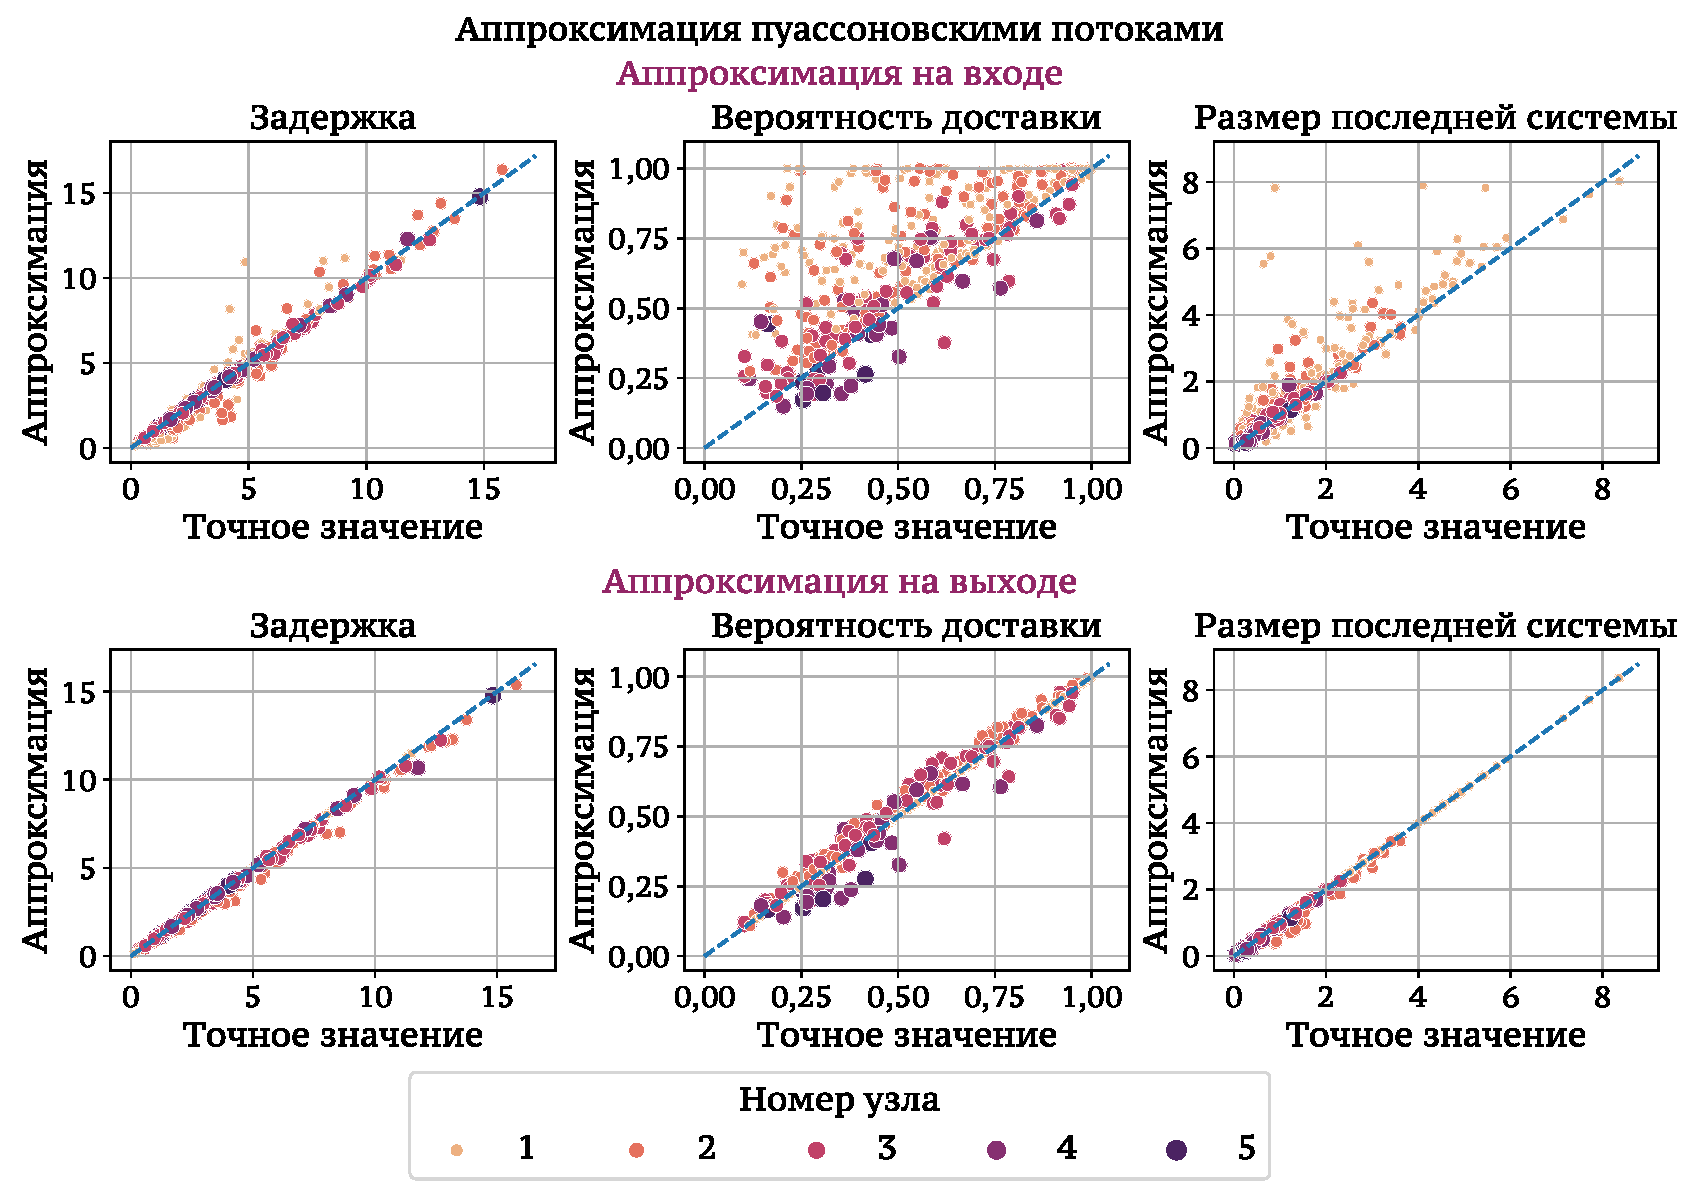
\includegraphics[width=0.90\textwidth]{chapter4/ch4_scatter_ph1}
  }
  \caption{Разброс оценок, полученных аппроксимацией потоков экспоненциальным распределением}
  \label{fig:ch4_scatter_ph1}
\end{figure}

Вполне ожидаемо, аппроксимация входящего потока ведет к очень серьезным отклонениям, особенно вероятности доставки и оценки размера последней системы. В обоих случаях чаще всего получается завышенная оценка, особенно для сетей малого размера. Отметим, что разброс оценок суммарной задержки не так велик. Также отметим, что разброс оценок в случае, когда аппроксимировались только выходящие потоки, оаказался относительно небольшим.

\begin{figure}[h]
  \centerfloat{
    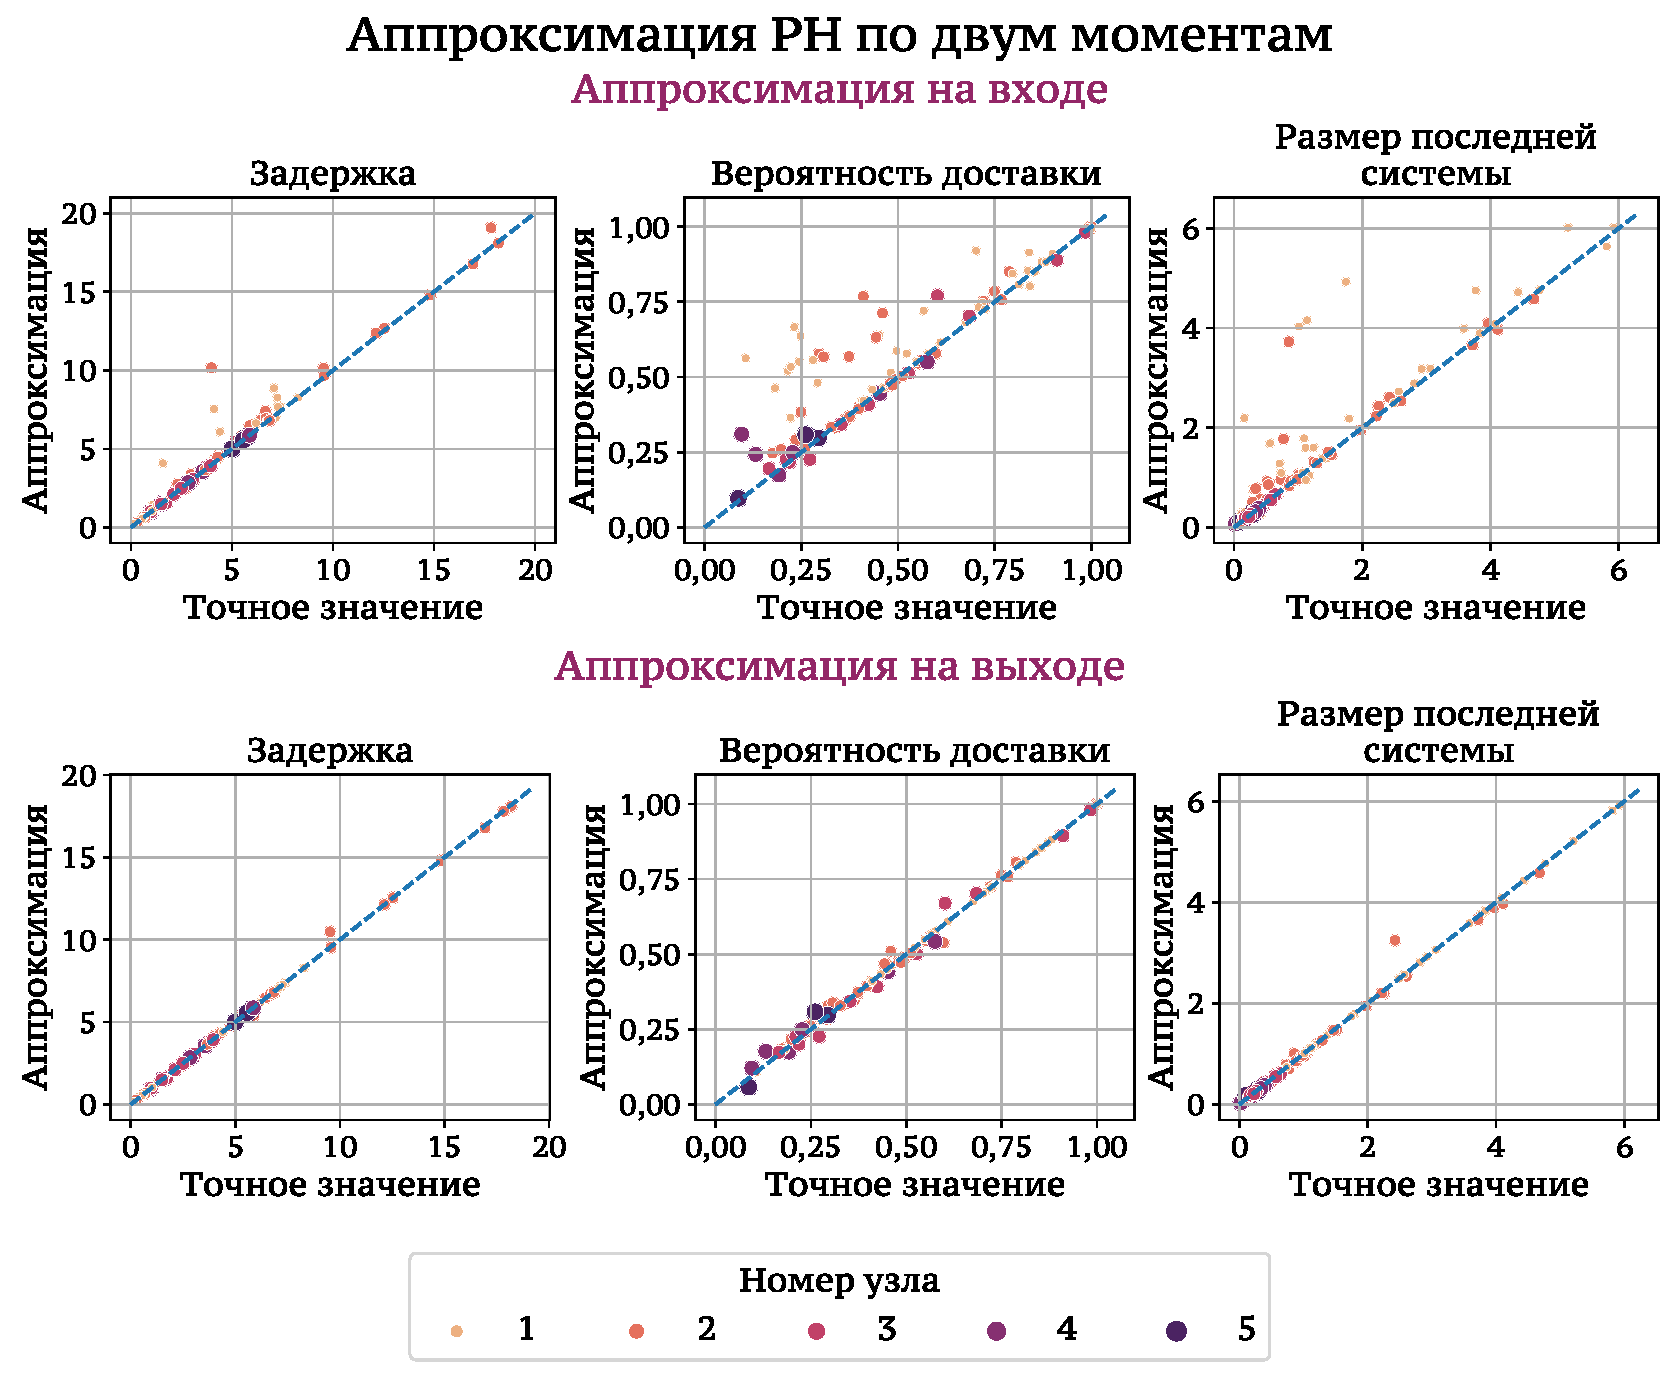
\includegraphics[width=0.90\textwidth]{chapter4/ch4_scatter_ph2}
  }
  \caption{Разброс оценок, полученных аппроксимацией потоков PH-распределениями по двум моментам}
  \label{fig:ch4_scatter_ph2}
\end{figure}

Далее было проведено сравнение с оценками, полученными аппроксимацией потоков с помощью PH-распределений по среднему и коэффициенту вариации (см. рис.~\ref{fig:ch4_scatter_ph2}). Как и в случае с аппроксимацией потоками Пуассона, ошибки при аппроксимации входящего MAP-потока оказались существенно больше ошибок, полученных в случае аппроксимации только выходящих потоков. В то же время отметим, что разброс немного снизился по сравнению с аппроксимациями потоками Пуассона.

\begin{figure}[h]
  \centerfloat{
    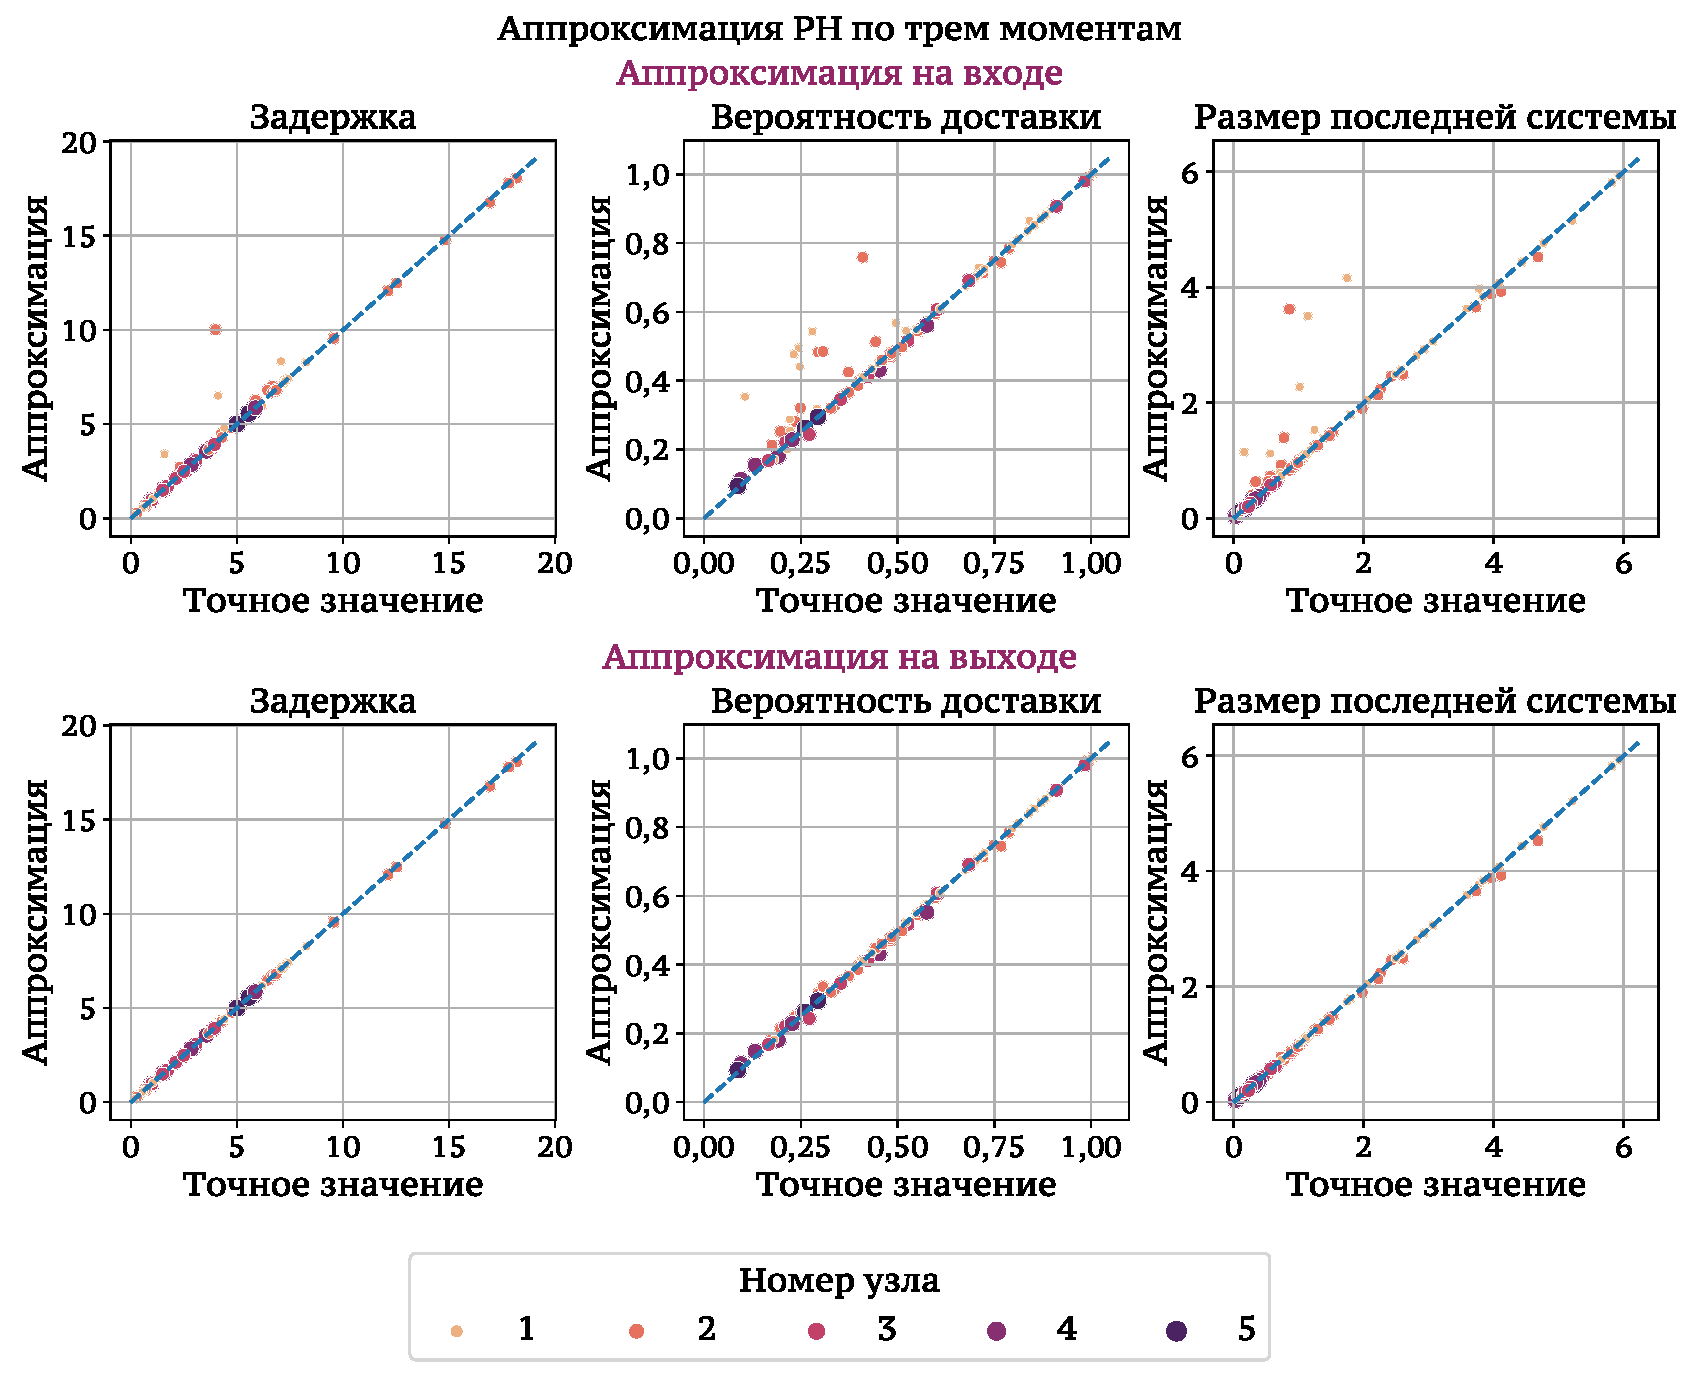
\includegraphics[width=0.90\textwidth]{chapter4/ch4_scatter_ph3}
  }
  \caption{Разброс оценок, полученных аппроксимацией потоков PH-распределениями по трем моментам}
  \label{fig:ch4_scatter_ph3}
\end{figure}

На рис.~\ref{fig:ch4_scatter_ph3} показаны результаты, полученные аппроксимацией MAP-потоков PH-распределениями по трем моментам. В этом случае, как и ранее, разброс при аппроксимации входящего потока выше разброса в случае аппроксимации только выходящих потоков, однако он существенно меньше, чем тот, что был получен предыдущими методами. Это наблюдение говорит о важности учета коэффициента асимметрии и, в то же время, о том, что отказ от учета автокорреляции входящего MAP-потока все же ведет к росту ошибок. Стоит отметить, что разброс оценок при аппроксимации только выходящих потоков очень мал.

Чтобы учесть автокорреляцию, использовался метод аппроксимации потоков новыми MAP-потоками, построенными по трем моментам и коэффициенту корреляции, который был описан в разделе~\ref{sec:ch4_approx_m3_lag1}. Разброс оценок показан на рис.~\ref{fig:ch4_scatter_map}. Полученный разброс мало отличается как в случае аппроксимации исходного MAP-потока, так и в случае аппроксимации только выходящих MAP-потоков.

\begin{figure}[h]
  \centerfloat{
    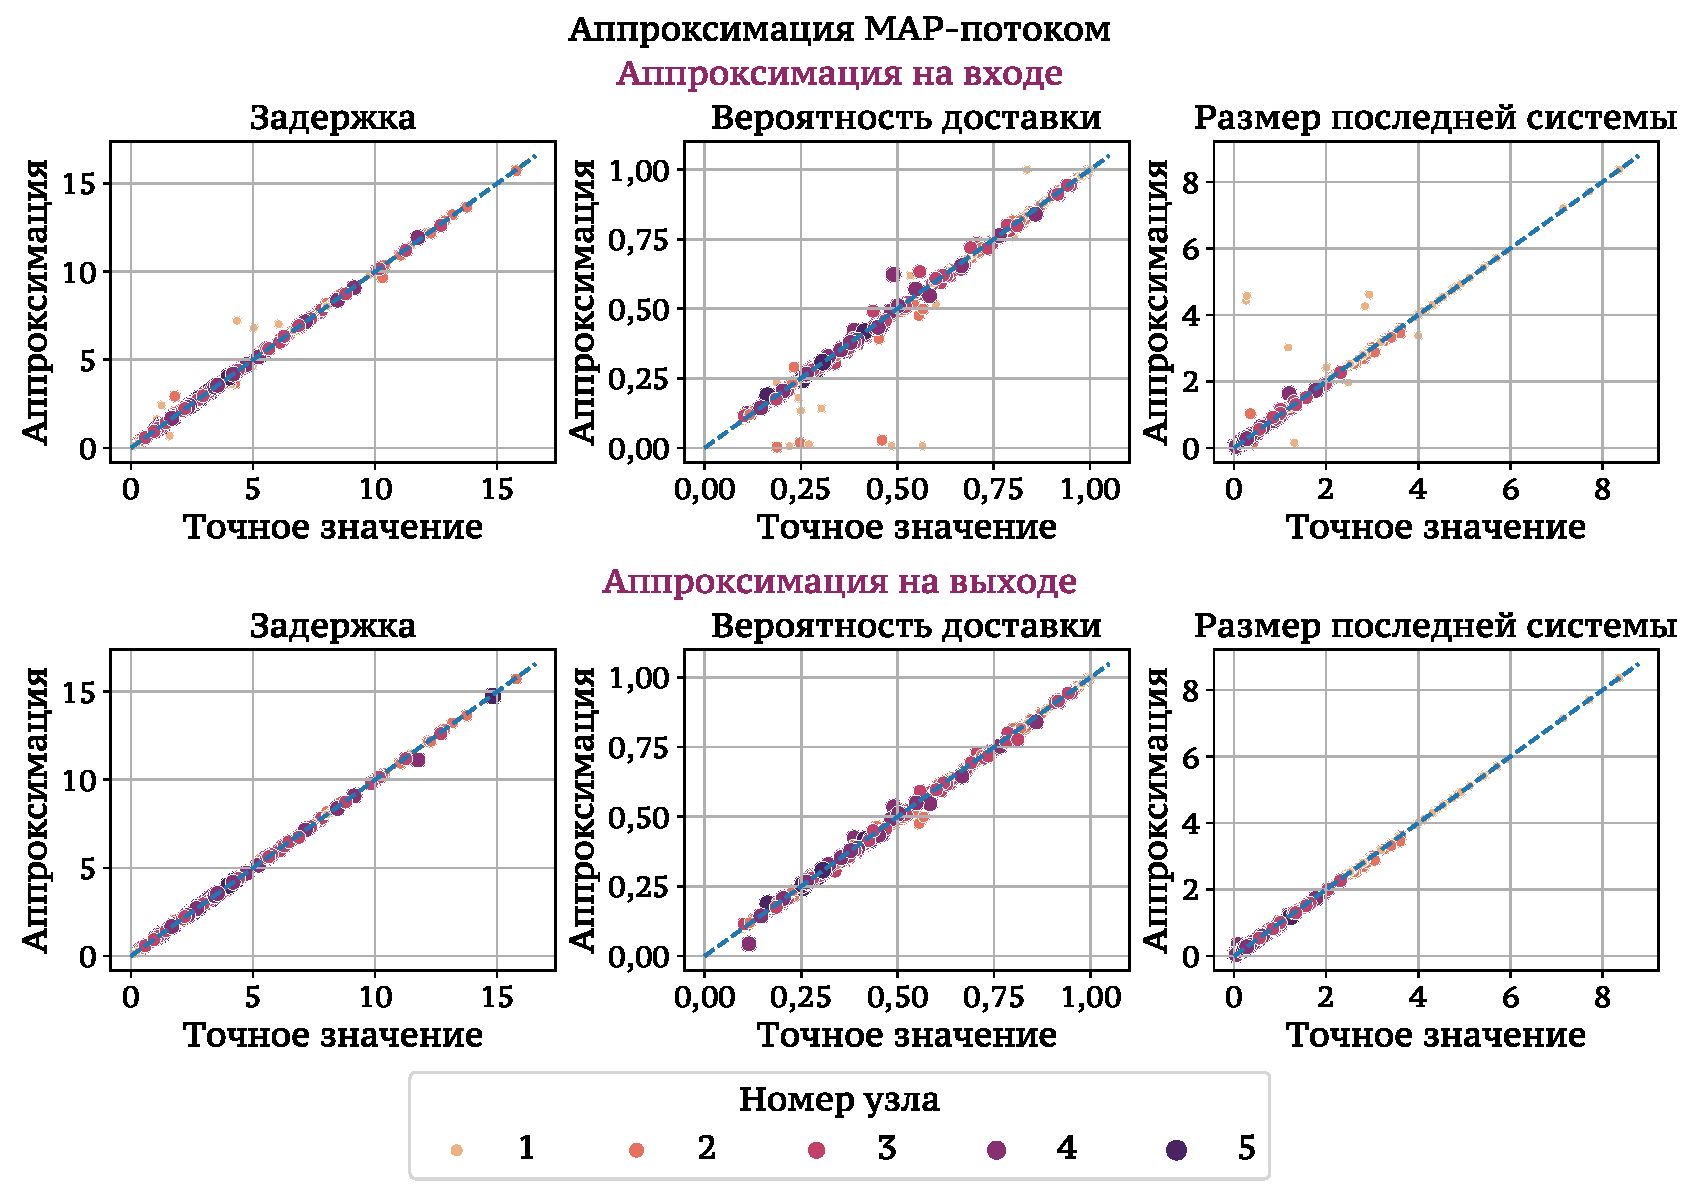
\includegraphics[width=0.9\textwidth]{chapter4/ch4_scatter_map}
  }
  \caption{Разброс оценок, полученных аппроксимацией MAP-потоков MAP-потоками по трем моментам и коэффициенту автокорреляции}
  \label{fig:ch4_scatter_map}
\end{figure}

Отметим, что последний результат может быть не совсем точным, так как для генерации MAP-потоков и их аппроксимации использовались одинаковые алгоритмы. Другими словами, исходные MAP-потоки имели достаточно <<хорошую>> структуру, чтобы быть точно аппроксимируемыми. Вероятно, ошибка при аппроксимации исходных MAP-потоков может увеличиться на более реалистичных данных (например, если исходные MAP-потоки обладают значительно автокорреляцией с большими лагами или существенно иной структурой переходов в матрице $D_0$).

На рис.~\ref{fig:ch4_scatter_monte_carlo} показан разброс оценок, полученных методом Монте-Карло. Для их получения в каждой сети моделировалось по 100 тысяч пакетов. Точность результатов оказывается наиболее высокой.

\begin{figure}[h]
  \centerfloat{
    \includegraphics[width=0.9\textwidth]{chapter4/ch4_scatter_monte_carlo}
  }
  \caption{Разброс оценок, полученных методом Монте-Карло}
  \label{fig:ch4_scatter_monte_carlo}
\end{figure}

Общий разброс ошибок, полученных всеми перечисленными методами, показан на рис.~\ref{fig:ch4_approximations_summary} с помощью диаграмм типа ящики с усами. На каждом ящике с усами средняя линия соответствует медиане ($Q_2$), нижняя и верхняя границы прямоугольника "--- первый ($Q_1$) и третий ($Q_3$) квартили, а границы усов определяются, как наименьшее значение выборки, не меньшее $Q_1 - 1.5 (Q_3 - Q_1)$, и наибольшее значение, не большее $Q_3 + 1.5 (Q_3 - Q_1)$. Точки, лежащие над верхним усом "--- выбросы.

\begin{figure}[!h]
  \centerfloat{
    \includegraphics[width=0.80\textwidth]{chapter4/ch4_approximations_summary}
  }
  \legend{На каждом ящике с усами средняя линия соответствует медиане ($Q_2$), нижняя и верхняя границы прямоугольника -- первый ($Q_1$) и третий ($Q_3$) квартили, а границы усов определяются, как наименьшее значение выборки, не меньшее $Q_1 - 1.5 (Q_3 - Q_1)$, и наибольшее значение, не большее $Q_3 + 1.5 (Q_3 - Q_1)$. Точки, лежащие над верхним усом - выбросы.}
  \caption{Точность оценок, полученных с помощью методов аппроксимации потоков и метода Монте-Карло}
  \label{fig:ch4_approximations_summary}
\end{figure}

Из приведенных на рис.~\ref{fig:ch4_approximations_summary} данных можно сделать несколько выводов. Во-первых, ожидаемо, метод Монте-Карло дает наилучшую оценку, причем среднее не значительно выше медианы. Это говорит о том, что даже имеющиеся выбросы относительно невелики и не утягивают среднее значение вверх слишком сильно. Средняя погрешность по всем трем метрикам находится в пределах 1,5\%. Во-вторых, аппроксимация входящего MAP дает существенно большую ошибку, особенно при использовании одного или двух моментов, что подтверждает важность учета коэффициента автокорреляции. В-третьих, ошибки в оценке суммарной задержки оказались невысокими даже при аппроксимации потоками Пуассона "--- меньше 10\% в среднем для сетей длиной два и более узла. В-четвертых, вероятность доставки и средний размер последней системы удается оценить с медианной погрешностью менее 10\% при аппроксимации MAP-потоков PH-распределениями по трем моментам и, естественно, MAP-потоками по трем моментам и коэффициенту автокорреляции. В-пятых, погрешности в оценке размеров системы и вероятности доставки становятся тем меньше, чем больше узлов в сети. Наконец, в-шестых, во всех случаях при аппроксимации потоков возникают редкие выбросы, которые очень сильно повышают среднее значение. Другими словами, в подавляющем большинстве случаев удается получить оценки с небольшой погрешностью (например, около 5\% для аппроксимации PH по трем моментам), но в редких случаях ошибка аппроксимации настолько велика, что срдняя ошибка по всему множеству входных наборов достигает 20\%.

\begin{figure}[h]
  \centerfloat{
    \includegraphics[width=0.90\textwidth]{chapter4/ch4_departure_autocorr}
  }
  \caption{Изменение коэффициентов автокорреляции и вариации в выходном потоке для системы MAP/PH/1/M}
  \label{fig:ch4_departure_autocorr}
\end{figure}

Рост ошибки при аппроксимации входящего MAP-потока, высокая точность Монте-Карло и улучшение приближений по мере увеличения числа аппроксимиируемых моментов были ожидаемы. В то же время, снижение ошибки при увеличении длины сети, а также практически идентичная точность при аппроксимации MAP-потоками и PH-распределениями по трем моментам, выглядят несколько неожиданно. Чтобы лучше понять причины этих наблюдений, рассмотрим, как меняется коэффициент автокорреляции и коэффициент вариации в выходном потоке. На рис.~\ref{fig:ch4_departure_autocorr} показан разброс коэффициентов автокорреляции и вариации во входном и выходном потоках. Во-первых, при положительной автокорреляции входящего потока, в выходящем потоке она снижается. Это правило нарушает только одно наблюдение. При нулевой автокорреляции во входящем потоке, в выходящем потоке она также снижается в большинстве случаев, хотя иногда (при высокой загрузке и положительной вариации и обслуживания, и входящего потока) может немного повыситься. Во-вторых, коэффициент вариации также меняется: если во входящем потоке вариация была больше единицы, то при относительно небольшой загрузке она уменьшается. Если же коэффициент вариации был меньше единицы (например, в случае распределений Эрланга), то вариация повышается, причем тем больше, чем выше загрузка. Такую связь с загрузкой можно объяснить тем, что когда поступления происходят чаще обслуживания (система насыщенна), на выходе наблюдается скорее распределение времени обслуживания, чем распределение интервалов между поступлениями.

\begin{figure}[h]
  \centerfloat{
    \includegraphics[width=0.85\textwidth]{chapter4/ch4_net_departure_autocorr}
  }
  \caption{Изменение коэффициентов автокорреляции и вариации в выходящих потоках на разных узлах сети}
  \label{fig:ch4_net_departure_autocorr}
\end{figure}

Еще более интересно отметить, что на последующих узлах сети изменения коэффициента автокорреляции и коэффициента вариации существеенно снижаются. Результаты, вычисленные для первых трех станций, показаны на рис.~\ref{fig:ch4_net_departure_autocorr}. Коэффициент автокорреляции также имеет тенденцию к снижению, однако его изменение становится тем меньше, чем дальше от начала сети находится узел. Коэффициент вариации также меняется тем меньше, чем дальше узел. Это позволяет понять, почему ошибки при аппроксимации выходящих потоков уменьшаются с ростом длины сети: ошибка при аппроксимации потоков на выходе с первого и второго узла может быть большой, однако далее она снижается, и общая ошибка растет медленнее по мере увеличения длины сети.

\begin{figure}[h]
  \centerfloat{
    \includegraphics[width=0.90\textwidth]{chapter4/ch4_scatter_monte_carlo_vs_ph3}
  }
  \caption{Сравнение оценок, полученных методами Монте-Карло и аппроксимацией только выходящих потоков PH-распределениями по трем моментам}
  \label{fig:ch4_scatter_monte_carlo_vs_ph3}
\end{figure}

Так как наиболее точные результаты из всех методов аппроксимации были получены для аппроксимации выходящих потоков PH-распределениями по трем моментам и MAP-потоками, также была исследована точность аппроксимации относительно метода Монте-Карло. Разброс оценок для всех (и простых, и сложных) входных данных показан на рис.~\ref{fig:ch4_scatter_monte_carlo_vs_ph3}.

Судя по полученным результатам, аппроксимацию PH-распределениями по трем моментам можно использовать для получения приближенных оценок характеристик тандемной сети.


%%% ~~~~~~~~~~~~~~~~
% \subsection{Влияние коэффициента асимметрии}
%%% ~~~~~~~~~~~~~~~~

% Одна из особенностей, на которую стоит обратить внимание "--- существенное влияние коэффициента асимметрии при аппроксимации выходящих потоков. Погрешность, полученная при использовании аппроксимации выходящих потоков с помощью PH-распределений по двум и трем моментам, отличается более, чем в два раза (см. рис.~\ref{fig:ch4_results_approx_summary}). Для более глубокого понимания зависимостей были проведены расчеты задержек и вероятностей успешной доставки в зависимости от коэффициентов асимметрии входящего потока (см. рис.~\ref{fig:ch4_results_arrival_skewness}) и распределения времени обслуживания (см. рис.~\ref{fig:ch4_results_service_skewness}) при различных коэффициентах вариации.

% \begin{figure}[h]
%   \centerfloat{
%     \includegraphics[width=0.8\textwidth]{chapter4/ch4_results_arrival_skewness.pdf}
%   }
%   \caption{Влияние коэффициента асимметрии входящего потока на задержку и вероятность доставки в системе MAP/PH/1/M}
%   \label{fig:ch4_results_arrival_skewness}
% \end{figure}

% В этих экспериментах рассматривался один узел MAP/PH/1/M с коэффициентом загрузки 0,5 ($m_a = 1, m_s = 0,5$) и емкостью очереди $M = 6$. Для исследуемого распределения (интервалов во входящем потоке или времени обслуживания) рассматривались четыре значения коэффициента вариации $c_{a,s} = \{0,9; 1; 2; 3\}$, а для другого распределения (соответственно, времени обслуживания и интервалов во входящем потоке) коэффициент полагался равным $c_{s,a} = 0,9$. Коэффициент асимметрии для исследуемого распределения менялся в интервале $[c_{a,s} - 1/c_{a,s}, 100]$, а для зафиксированного полагался равным $c_{s,a} - 1/c_{s,a} = -19/90$.

% \begin{figure}[h]
%   \centerfloat{
%     \includegraphics[width=0.8\textwidth]{chapter4/ch4_results_service_skewness.pdf}
%   }
%   \caption{Влияние коэффициента асимметрии распределения времени обслуживания на задержку и вероятность доставки в системе MAP/PH/1/M}
%   \label{fig:ch4_results_service_skewness}
% \end{figure}

% Из приведенных результатов можно сделать несколько выводов. Во-первых, коэффициент асиммтерии входящего потока сильно влияет на характеристики системы, причем влияние тем сильнее, чем выше коэффициент вариации, а для $c_a > 1$ нужно учитывать конкретные значения $\gamma_a$ даже при $\gamma_a \gg 1$ (см. кривые на рис.~\ref{fig:ch4_results_arrival_skewness} при $c_a = 2,0, 3,0$). Во-вторых, коэффициент асиммтерии времени обслуживания также оказывает влияние, но меньшее, и при росте $\gamma_s$ больше некоторого значения $\underline{\gamma_s} = \underline{\gamma_s}(c_s)$, зависящего от коэффициента варации $c_s$, это влияние практически пропадает. В рассмотренном случае можно приблизительно оценить эти значения как $\underline{\gamma_s}(1) = \underline{\gamma_s}(0.9) \approx 15$, $\underline{\gamma_s}(2) \approx 25$ и $\underline{\gamma_s}(3) \approx 55$ (см. рис.~\ref{fig:ch4_results_service_skewness}). Таким образом, чем больше вариация, тем больший диапазон асимметрии надо учитывать.

% Если коэффициент асимметрии входящего потока существенно влияет и на задержку, и на вероятность доставки, то коэффициент асимметрии времени обслуживания влияет существенно сильнее на вероятность доставки, чем на задержку. Так, в исследуемом случае задержка практически не меняется для любых $\gamma_s > 15$. В то же время, при небольших значениях $\gamma_s < 15$ влияние на задержку также достаточно сильное, причем тем больше, чем выше коэффициент вариации $c_s$. Отметим, что конкретные виды зависимости могут отличаться в зависимости от коэффициента загрузки $m_s / m_a$, емкости очереди $M$ и коэффициентов автокорреляции.

% Из приведенных численных результатов можно сделать вывод, что при аппроксимациях выходящих потоков, а также при поиске подходящего распределения времени обслуживания (например, если требуется описать время передачи пакетов в канале связи) важно учитывать коэффициент асимметрии. В частности, будем далее руководствоваться этим результатом при построении моделей каналов беспроводных сетей.


%%% ~~~~~~~~~~~~~~~~
\subsubsection{Скорость вычислений и сходимость метода Монте-Карло}
%%% ~~~~~~~~~~~~~~~~

\begin{figure}[h]
  \centerfloat{
    \includegraphics[width=0.90\textwidth]{chapter4/ch4_approximations_elapsed}
  }
  \caption{Длительность расчета точного решения, а также расчетов с помощью различных методов аппроксимации выходящих потоков и метода Монте-Карло}
  \label{fig:ch4_approximations_elapsed}
\end{figure}

Для всех методов аппроксимации, точного решения и метода Монте-Карло были проведены измерения времени, необходимого для получения оценок, результаты показаны на рис.~\ref{fig:ch4_approximations_elapsed}. Можно отметить, во-первых, что точное решение требует больше всего времени. Это связано с необходимостью обращать матрицы и решать системы линейных уравнений очень высокого порядка (размеры матриц были ограничены 8000-ми строк/столбцов). Во-вторых, аппроксимация MAP-потоками также работает долго. Причина "--- необходимость решать задачу оптимиазации для поиска элементов матрицы $D_1$ (поиск минимума и максимума допустимых коэффициентов автокорреляции для заданной матрицы $D_0$). В-третьих, остальные методы аппроксимации работают быстрее метода Монте-Карло. Так, если для сетей с 9 узлами метод Монте-Карло требует порядка 200--300~мс., то аппроксимация PH-распределениями по трем моментам -- около 150~мс., а аппроксимация PH-распределениями по одному или двум моментам -- менее 50~мс. Отметим, что все численные эксперименты проиводились на рабочей станции с процессором Intel Core i7-9700K под управлением ОС Ubuntu Linux. Код имитационной модели компилировался с помощью компилятора GCC с уровнем оптимизации O3. Расчет методом аппроксимации потоков был реализован на Python с использованием библиотек NumPy и SciPy.

\begin{figure}[h]
  \centerfloat{
    \includegraphics[width=0.90\textwidth]{chapter4/ch4_monte_carlo_performance}
  }
  \caption{Сходимость метода Монте-Карло и скорость выполнения расчетов}
  \label{fig:ch4_monte_carlo_performance}
\end{figure}

Наконец, отметим, что 100 тыс. пакетов для метода Монте-Карло является даже избыточным. На рис.~\ref{fig:ch4_monte_carlo_performance} показано, как меняется точность результатов от числа промоделированных пакетов, а также то, как меняется время, расходуемое на выполнение метода. Так, для получения точности 5~\% оказывается достаточно промоделировать около 50 тыс. пакетов. Ограничить число пакетов представляется разумным в свете того, что необходимое время зависит от числа пакетов почти линейно.




%%%%%%%%%%%%%%%%%%%%%%%%%%%%%%%%%%%%%%%%%%%%%%%%%%%%%%%%%%%%%%%%%%%%%%%%%%%%%%%%
\section{Численный расчёт характеристик многошаговой беспроводной сети}\label{sec:ch4_results_networks}
%%%%%%%%%%%%%%%%%%%%%%%%%%%%%%%%%%%%%%%%%%%%%%%%%%%%%%%%%%%%%%%%%%%%%%%%%%%%%%%%

В численном эксперименте были исследованы характеристики многошаговых беспроводных сетей с помощью метода, описанного в разделе~\ref{sec:ch4_wireless_network_model}. Предполагалось, что сеть работает в ad-hoc режиме по стандарту IEEE 802.11 DCF без RTS/CTS. Параметры настройки протокола приведены в табл.~\ref{table:ch4_channel_parameters}. Беспроводная сеть моделировалась в системе моделирования NS-3, в каждом запуске моделировалась передача 500'000 пакетов.

\begin{table}[h!]\centering{
\begin{tabular}{|c|c|c|c|}\hline
Параметр & Значение & Единицы\\ \hline
Заголовок PHY & 128 & бит\\
Заголовок MAC DATA & 208 & бит \\
Кадр MAC ACK & 96 & бит \\
Слот ($\sigma$) & 9 & мкс \\
DIFS & 34 & мкс\\
SIFS & 16 & мкс \\
CWmin & 16 & - \\
CWmax & 1024 & - \\
Скорость канала & 54 & мбит/с \\
Заголовок IP & 160 & бит \\ \hline
Средний размер пакета данных ($\overline{\xi}$) & 11200 & бит\\
Минимальная интенсивность трафика ($B_\text{min}$) & 1,2 & мбит/с \\
Максимальная интенсивность трафика ($B_\text{max}$) & 12 & мбит/с \\ \hline
\end{tabular}\caption{Параметры беспроводных каналов и трафика для эксперимента}\label{table:ch4_channel_parameters}
}\end{table}

Входящий трафик моделировался пуассоновскими потоками с четырьмя интенсивностями $\lambda = 100, 200, 500, 750, 1000$. Учитывая, что средний размер пакетов, поступающих от пользователей, был равен 11200~бит, эти потоки соответствовали трафику $1,2$, $2,4$, 6, 9 и 12 мегабит в секунду.

%%% ~~~~~~~~~~~~~~~~
\subsection{Характеристики каналов калибровочной сети}
%%% ~~~~~~~~~~~~~~~~

Для получения PH-распределений, моделирующих время передачи пакетов в каналах, с помощью имитационной модели в NS-3 была собрана статистика длительностей передачи пакетов в каждом из четырех каналов калибровочной сети, показанной на рис.~\ref{fig:ch4_channel_model_schema}. Характеристики длительностей передач пакетов для $\lambda = 500$ показаны на рис.~\ref{fig:ch4_ns3_calibration_links_densities}.

\begin{figure}[h]
  \centerfloat{
    \includegraphics[width=0.85\textwidth]{chapter4/ch4_ns3_calibration_links_densities}
  }
  \caption{Распределение длительностей передач пакетов в каналах калибровочной сети для $\lambda = 500$.}
  \label{fig:ch4_ns3_calibration_links_densities}
\end{figure}

Можно видеть, что по мере удаления от источника коэффициент вариации падает, распределение становится все ближе к константе.
Как можно видеть из рис.~\ref{fig:ch4_ns3_calibration_links_koefs}, это наблюдение справедливо практически для всех интенсивностей, кроме $\lambda = 750$.

\begin{figure}[h]
  \centerfloat{
    \includegraphics[width=0.85\textwidth]{chapter4/ch4_ns3_calibration_links_koefs}
  }
  \caption{Средние длительности передач, коэффициенты вариации и асимметрии для каналов калибровочной сети.}
  \label{fig:ch4_ns3_calibration_links_koefs}
\end{figure}

С помощью метода восстановления PH-распределения по трем моментам, описанного в работе \cite{Johnson1989}, были построены PH-распределения для каждого канала калибровочной сети и рассчитаны межконцевые задержки с помощью сети массового обслуживания M/$\text{PH}_1$/1/N $\rightarrow \bullet$/$\text{PH}_2$/1/N $\rightarrow \bullet$/$\text{PH}_3$/1/N$ \rightarrow \bullet$/$\text{PH}_4$/1/N. Эти значения сравнивались со значениями задержек, полученных из имитационной модели калибровочной сети в NS-3. Для того, чтобы исследовать целесообразность использования сложных моделей PH-распределений, задержки также были найдены с помощью простой модели типа M/$\text{M}_1$/1/N $\rightarrow \dots \rightarrow \bullet$/$\text{M}_4$/1/N, в которой обслуживание моделировалось экспоненциальными распределениями, которые были найдены по средним длительностям передач пакетов в каналах. Результаты сравнения приведены на рис.~\ref{fig:ch4_ns3_calibration_delays}.

\begin{figure}[h]
  \centerfloat{
    \includegraphics[width=0.85\textwidth]{chapter4/ch4_ns3_calibration_delays}
  }
  \caption{Межконцевые задержки в калибровочной сети}
  \label{fig:ch4_ns3_calibration_delays}
\end{figure}

Для интенсивностей $\lambda = 100, 200, 1000$ ошибки не превышают 10~\%, причем для $\lambda = 100, 200$ тандемы с PH-распределениями времени обслуживания оказываются в полтора раза точнее, а для $\lambda = 1000$ немного более точный результат дают экспоненциальные распределения. Для $\lambda = 500$ ошибка составила 15~\% для экспоненциальных распределений и 24~\% для PH-распределений. Что касается $\lambda = 750$, ошибка достигла почти 96~\%. Возможная причина "--- особенности работы модели NS-3. Так, в выборке длительностей передач оказывались пакеты, которые доставлялись более секунды, хотя они должны были бы быть отброшены из-за исчерпания попыток передач. В дальнейшем рассматривались только $\lambda = 100, 200, 500, 1000$.


%%% ~~~~~~~~~~~~~~~~
\subsection{Расчет межконцевых задержек в сети произвольного размера}
%%% ~~~~~~~~~~~~~~~~

Для расчета межконцевых задержек в сети, состоящей из 10 станций, использовалась методика, описанная в разделе~\ref{sec:ch4_channel}: первый и два последних каналов моделировались распределениями, полученными для каналов $S_1 \rightarrow S_2$, $S_3 \rightarrow S_4$, $S_4 \rightarrow S_5$ калибровочной сети, а все промежуточные "--- с помощью распределения, построенного для канала $S_2 \rightarrow S_3$ калибровочной сети (см. рис.~\ref{fig:ch4_network_model_schema}). Как и ранее, использовались две модели сетей массового обслуживания: с PH-распределениями и экспоненциальными распределениями. Результаты сравнения с данными, полученными из модели NS-3, показаны на рис.~\ref{fig:ch4_ns3_tandem_delays}.

\begin{figure}[h]
  \centerfloat{
    \includegraphics[width=0.85\textwidth]{chapter4/ch4_ns3_tandem_delays}
  }
  \caption{Межконцевые задержки в сети из 10 станций, рассчитанные с помощью оригинальной методики}
  \label{fig:ch4_ns3_tandem_delays}
\end{figure}

Полученные результаты показывают, что обе модели дают неплохое приближение межконцевой задержки, причем сеть массового обслуживания с PH-распределениями точнее аппроксимирует беспроводную сеть. Стоит отметить, что для расчета характеристик сети массового обслуживания требовалось значительно меньше времени, чем на выполнение имитационной модели в NS-3. В то же время, ошибка растет по мере роста размера сети, особенно при высокой интенсивности входящего потока. Причем если в сети массового обслуживания рост задержки практически линеен, то в беспроводной сети скорость роста задержки снижается по мере роста размера сети.

\begin{figure}[h]
  \centerfloat{
    \includegraphics[width=0.85\textwidth]{chapter4/ch4_ns3_net_10_props}
  }
  \caption{Характеристики распределений длительностей передачи пакетов в каналах беспроводной сети из 10 станций}
  \label{fig:ch4_ns3_net_10_props}
\end{figure}

Для того, чтобы объяснить это наблюдение, на рис.~\ref{fig:ch4_ns3_net_10_props} показаны характеристики каналов беспроводной сети, состоящей из 10 станций. Можно видеть, что первые каналы испытывают наибольшую нагрузку "--- средние длительности передач в них самые большие, как и потери пакетов. По мере передачи трафика далее, часть пакетов теряется и на вход следующих станций поступает все более разреженный трафик, в результате чего конкуренция снижается и скорость передачи возрастает. Таким образом, из-за того, что для моделирования промежуточных каналов использовалось распределение времени передачи канала $S_2 \rightarrow S_3$ калибровочной сети, была введена систематическая ошибка.

\begin{figure}[h]
  \centerfloat{
    \includegraphics[width=0.8\textwidth]{chapter4/ch4_network_model_schema_refined}
  }
  \caption{Улучшенная схема моделирования беспроводной сети с произвольным числом станций}
  \label{fig:ch4_network_model_schema_refined}
\end{figure}

Можно немного изменить методику выбора распределений, чтобы лучше учесть этот эффект просеивания трафика по мере удаления от источника. Будем моделировать первые четыре канала точно теми же распределениями, что были получены для калибровочной сети, а все последующие каналы "--- распределением для канала $S_4 \rightarrow S_5$. Новая схема моделирования показана на рис.~\ref{fig:ch4_network_model_schema_refined}.

\begin{figure}[h]
  \centerfloat{
    \includegraphics[width=0.85\textwidth]{chapter4/ch4_ns3_tandem_delays_refined}
  }
  \caption{Межконцевые задержки в сети из 10 станций, рассчитанные с помощью улучшенной методики}
  \label{fig:ch4_ns3_tandem_delays_refined}
\end{figure}

С помощью обновленной схемы расчета были получены более точные оценки, используя, как и ранее, PH-распределения и экспоненциальные распределения времени передачи пакетов. Результаты показаны на рис.~\ref{fig:ch4_ns3_tandem_delays_refined}. Можно отметить, что теперь для $\lambda = 500$ сеть с экспоненциальными распределениями дала даже лучший результат, чем сеть с PH-распределениями. В остальных случаях использование PH-распределений по-прежнему дает более высокую точность.

\begin{figure}[h]
  \centerfloat{
    \includegraphics[width=0.85\textwidth]{chapter4/ch4_ns3_tandem_errors}
  }
  \caption{Ошибки оценок межконцевых задержек беспроводной сети с помощью моделей сетей массового обслуживания}
  \label{fig:ch4_ns3_tandem_errors}
\end{figure}

Ошибки, полученные с помощью исходной и улучшенной методики, приведены на рис.~\ref{fig:ch4_ns3_tandem_errors}. Обновленная методика дает более точное приближение межконцевых задержек, независимо от того, используется ли для моделирования длительностей передач пакетов экспоненциальное или PH-распределение. Ошибка, полученная с помощью обновленной методики, не превосходит 20~\%, кроме тандема с PH-распределениями при $\lambda = 500$. Во всех остальных случаях тандем с PH-распределениями, построенный по обновленной методике, дает самое лучшее приближение. При $\lambda = 500$ самые точные приближения были получены с помощью тандема с экспоненциальными распределениями, построенного по обновленной методике, и тандема с PH-распределениями, построенного по оригинальной методике.



%%%%%%%%%%%%%%%%%%%%%%%%%%%%%%%%%%%%%%%%%%%%%%%%%%%%%%%%%%%%%%%%%%%%%%%%%%%%%%%%
\section{Заключение}\label{sec:ch4_conclusion}
%%%%%%%%%%%%%%%%%%%%%%%%%%%%%%%%%%%%%%%%%%%%%%%%%%%%%%%%%%%%%%%%%%%%%%%%%%%%%%%%
В главе были представлены следующие результаты.

\begin{enumerate}
  \item Предложен метод нахождения приближенных значений характеристик открытых сетей массового обслуживания с узлами MAP/PH/1/N с помощью аппроксимации потоков обслуженных пакетов PH-распределениями и MAP-потоками меньшего порядка. Приведены результаты численного исследования метода, показывающие высокую точность при использовании PH-распределений, построенных по трем моментам исходного потока.
  \item Предложена методика построения и выбора распределений для моделирования многошаговых беспроводных сетей IEEE 802.11 произвольного размера с помощью тандемных сетей массового обслуживания.
  \item Представлены результаты численного исследования предложенной методики моделирования многошаговых беспроводных сетей, показывающие высокую точность получаемых оценок межконцевых задержек.
\end{enumerate}


\clearpage
           % Глава 4
% \chapter{Разработка и экспериментальное внедрение системы радиочастотной идентификации}\label{ch:ch5}
Важная задача, возникающая при построении системы радиочастотной идентификации транспортных средств "--- необходимость объединять в реальном времени данные со множества считывателей, которые могут быть размещены на большой территории. Для решения этой задачи была разработана распределенная платформа для интеграции и управления RFID-считывателями. Платформа позволяет интегрировать разрозненные считыватели в единую масштабируемую систему обработки данных.

В 2014--2015 годах был проведён эксперимент в городе Казань, в ходе которого было проведено испытание разработанной платформы и RFID-считывателей для идентификации меток, размещённых на рейсовых автобусах. Весной 2020 года совместно с АО <<Микрон>> в рамках НИР были проведены испытания на полигоне в городе Казань для проверки системы при идентификации меток на автомобилях, движущихся со скоростями до 170~км/ч. Все испытания завершились успешно. Летом 2021 года начались испытания на платном участке центральной кольцевой автодороги (ЦКАД), которые к моменту написания диссертации еще не завершились.

В этой главе приводится описание разработанной платформы и проведенных экспериментальных исследований. В разделе \ref{sec:ch5_architecture} описывается структура платформы управления считывателями и ее основные компоненты, в разделе \ref{sec:ch5_protocols} "--- разработанные протоколы, а в разеделе \ref{sec:ch5_components} "--- модули системы. Далее, в разделе \ref{sec:ch5_implementation}, описывается аппаратная реализация RFID-считывателей и особенности программной реализации. Раздел \ref{sec:ch5_experiments} посвящен описанию экспериментальных исследований разработанных RFID-считывателей и системы управления. Заключение в разделе \ref{sec:ch5_conclusion} завершает главу.

Результаты, представленные в главе, были опубликованы в работах, индексируемых Scoupus/WoS \cite{RFIDCTRL_NETS2CARS2014, RFIDTA2012}, и представлены в трудах конференций \cite{RFIDCTRL_DCCN2017, RFIDCTRL_VSPU2014}. По результатам эксперимента 2020 года был сделан доклад на форуме Kazan Digital Week 2020.


%%%%%%%%%%%%%%%%%%%%%%%%%%%%%%%%%%%%%%%%%%%%%%%%%%%%%%%%%%%%%%%%%%%%%%%%%%%%%%%%
\section{Архитектура системы управления считывателями}\label{sec:ch5_architecture}
%%%%%%%%%%%%%%%%%%%%%%%%%%%%%%%%%%%%%%%%%%%%%%%%%%%%%%%%%%%%%%%%%%%%%%%%%%%%%%%%
Радиочастотная идентификация транспорта может применяться для идентификации автомобилей в системах регистрации нарушений правил дорожного движения, для оплаты проезда по платным дорогам, доступа на закрытые территории, а также использоваться при поиске угнанных машин и розыске преступников. Для быстрой реализации различных приложений программное обеспечение должно предоставлять возможность простого добавления новых сервисов в систему, а также обеспечивать масштабируемость.

\begin{figure}[ht]
  \centerfloat{
    \includegraphics [width=0.5\textwidth]{chapter5/ch5_components}
  }
  \caption{Компоненты системы управления}
  \label{fig:ch5_components}
\end{figure}

Система управления считывателями имеет модульную структуру (см. рис.~\ref{fig:ch5_components}) и включает три типа модулей: супервайзеры, RFID-адаптеры и приложения. Супервайзеры (SVR) отвечают за хранение и управление конфигурацией системы. RFID-адаптеры управляют работой радиомодулей RFID-считывателей, реализуют чтение и запись меток. Приложения обрабатывают потоки прочитанных меток, поступающих от RFID-адаптеров и других приложений. Приложения могут использоваться для объединения потоков от нескольких источников, фильтрации или преобразования протоколов. Кроме перечисленных модулей, в состав системы входят иструменты администрирования "--- консоль и веб-интерфейс.

Каждый модуль системы поддерживает множество объектов, каждый из которых является либо параметром, либо процедурой. Обработка объектов ведётся по запросам, приходящим от пользователей или других модулей системы. Множество объектов полностью определяется типом модуля. Например, каждый RFID--адаптер поддерживает параметры <<температура радио--модуля>>, <<значение Q>>, <<номер сессии>> и процедуры <<выключить радио--модуль>>, <<включить радио--модуль>>. RFID--адаптер, специализированный на поддержке определенного считывателя, может предоставлять объекты, специфичные для конкретной модели считывателя. Каждый модуль получает свои настройки от супервайзера сразу после включения.

Для работы с объектом пользователь или модуль должны отправить запрос супервайзеру через один из поддерживаемых им протоколов управления (рассматриваются ниже). Супервайзер поддерживает множество собственных объектов, например "--- <<число активных пользователей>> или <<статус подключений модулей>>, а также выполняет проксирование объектов всех подключенных модулей. Когда супервайзер получает запрос на объект, который не принадлежит ему самому, он перенаправляет запрос модулю, которому этот объект принадлежит, и отвечает клиенту, перенаправляя ответ, полученный от модуля.

В системе используется разделение потоков данных и управления: все управление производится через супервайзер, а данные передаются напрямую между RFID-адаптерами и приложениями. Такое разделение позволяет, с одной стороны, снизить нагрузку на супервайзер и увеличить масштабируемость, а с другой "--- использовать более простые протоколы между компонентами. Так как основное назначение системы "--- непрерывное чтение меток проезжающих автомобилей, передача данных о прочитанных метках организована в виде потоков. Приложение, которое хочет получать данные о метках от RFID-адаптера или другого приложения должно подписаться на поток.

Пользователи могут настраивать систему и взаимодействовать с RFID-адаптерами и приложениями. В системе определены четыре уровня доступа: наблюдатели, операторы, администраторы и суперпользователи. Наблюдатели могут подписываться на потоки меток, но не могут записывать метки или менять настройки оборудования. Операторы имеют право настраивать RFID--адаптеры и выполнять операции чтения/записи меток, но не могут менять настройки остальных компонентов системы. Администраторы имеют право настраивать модули, но не могут записывать метки. Суперпользователи имеют права на любые действия с системой. Помимо уровней доступа пользователей с каждым компонентом связан специальный системный уровень доступа, который позволяет ему работать с определенным набором объектов других компонентов. Например, приложения могут читать, но не имеют права записывать параметры RFID--адаптеров.

Поскольку все модули системы взаимодействуют друг с другом по сети, физически они могут располагаться где угодно. Типичные примеры размещений модулей показаны на рис.~\ref{fig:ch5_deployments}.

\begin{figure}[ht]
  \centerfloat{
    \includegraphics [width=0.9\textwidth]{chapter5/ch5_deployments}
  }
  \caption{Примеры размещения модулей системы}
  \label{fig:ch5_deployments}
\end{figure}

Для обычного RFID--считывателя, построенного на базе среднего процессора (например, одноядерный ARM A7 или ARM A8), обладающего небольшим объемом оперативной памяти порядка 256--512~МБ и имеющего в составе один радиомодуль, достаточно установить супервайзер, RFID-адаптер, а также приложение для подключения к потоку прочитанных меток снаружи (TFPD) и модуль, предоставляющий доступ к настройке считывателя через веб-интерфейс или консоль. Такое размещение компонентов позволяет передавать данные обо всех прочитанных метках в центр обработки данных и, при необходимости, реализовывать операции чтения/записи через подключение внешних модулей и пользователей. Именно такая конфигурация считывателей использовалась во всех проведенных экспериментах.

Если считыватель имеет более мощное вычислительное ядро, на нём можно разместить несколько приложений. Например, на нем можно установить приложения для фильтрации прочитанных меток или нахождения соответствий с номерными знаками, распознанными камерами. Если считыватель включает несколько радиомодулей, то потребуется несольких RFID--адаптеров. Хотя каждый компонент системы не требователен к вычислительным ресурсам по отдельности, для выполнения задач обработки потоков меток могут потребоваться дополнительные ресурсы. Желательно использовать 2-х или 4-х ядерный процессор ARM и 512 "--- 1024 МБ оперативной памяти.

В наиболее сложном случае система может работать в распределенном режиме, а различные ее компоненты размещаться на считывателях и серверах, при этом считыватели могут быть сделаны чрезвычайно <<тонкими>> "--- на них достаточно разместить RFID--адаптер, который будет подключаться по сети к супервайзеру, работающему на внешнем сервере или в облаке. Приложения также могут работать на отдельных физических или виртуальных внешних серверах. В этом варианте считыватели могут быть реализованы на самых простых вычислительных компонентах, что позволит снизить их стоимость, а приложения и супервайзер выполняются в центре обработки данных на мощном вычислительном оборудовании, благодаря чему им можно поручить работу с большим числом считывателей. Такой вариант размещения наиболее гибок и позволяет построить распределенную систему, состоящую из сотен считывателей, каждый из которых может администрироваться из единой консоли.



%%%%%%%%%%%%%%%%%%%%%%%%%%%%%%%%%%%%%%%%%%%%%%%%%%%%%%%%%%%%%%%%%%%%%%%%%%%%%%%%
\section{Протоколы взаимодействия компонентов системы}\label{sec:ch5_protocols}
%%%%%%%%%%%%%%%%%%%%%%%%%%%%%%%%%%%%%%%%%%%%%%%%%%%%%%%%%%%%%%%%%%%%%%%%%%%%%%%%

В системе управления передача данных и управления разделены. Для упрвления системой были разработаны протоколы IMMP (Internal Modules Management Protocol) и SUAP (Simple User Access Protocol), а для передачи потоков меток и работы с радиомодулями "--- протоколы ITOP (Internal Tags Operation Protocol) и TFP (Tag Flow Protocol). Протоколы IMMP и ITOP используются для управления и передачи внутри системы, а протоколы SUAP и TFP "--- для работы работы с супервайзером со стороны интерфейсов управления и получения потоков прочитанных меток во внешние информационные системы. Все протоколы, используемые в системе, показаны на рис.~\ref{fig:ch5_protocols}.

\begin{figure}[ht]
  \centerfloat{
    \includegraphics [width=0.4\textwidth]{chapter5/ch5_protocols}
  }
  \caption{Протоколы передачи данных и управления}
  \label{fig:ch5_protocols}
\end{figure}

Все протоколы имеют клиент--серверную архитектуру, соединение создаётся клиентом. Каждый запрос должен подтверждаться получателем с помощью специального сообщения Response, содержащего результат обработки запроса или код ошибки. Запросы упорядочиваются с помощью порядкового номера ReqSN (Request Sequence Number): клиент и сервер поддерживают счетчики, перед отправкой значение счетчика увеличивается и помещается в соответствующее поле в запросе. В ответе на запрос поле ReqSN должно совпадать со значением счетчика из запроса. Этот механизм позволяет реализовать асинхронную обработку запросов "--- отправителю запроса не нужно ждать ответа для того, чтобы передать новый запрос. При этом отправитель может быть уверен, что запросы будут обработаны в порядке их передачи: если получатель видит, что номер запроса меньше последнего обработанного, запрос будет проигнорирован. С каждым запросом также связано максимальное ожидание ответа, после которого отправитель считает, что запрос не был выполнен.

Формат сообщений, кодируемых с помощью ASCII-строк, аналогичен форматам, используемым в HTTP v1.1 и SIP.


%%% --------------------------------------------
\subsection{IMMP "--- протокол управления модулями}\label{sec:ch5_immp}
%%% --------------------------------------------

Протокол IMMP работает поверх транспортного уровня TCP и реализует функции получения модулями своей начальной конфигурации от супервайзера, получения и установки значений параметров модулей, а также удалённый вызов процедур. В роли сервера всегда выступает супервайзер, а клиента "--- один из модулей системы.

В протоколе определены семь запросов: HELLO, ACK, BYE, GET, SET и CALL. Запрос HELLO отправляется клиентом для создания соединения. Если соединение может быть установлено, сервер (супервайзер) сначала передает ответ с кодом успеха (200), а затем "--- запрос ACK, в котором передает конфигурацию модуля и случайный ключ сессии (SKey, Session Key), по которому в дальнейшем он будет авторизовывать запросы этого клиента. Запросы GET и SET используются для чтения и записи значений объектов--параметров, а запрос CALL "--- для удаленного вызова процедур. Запросы GET, SET и CALL могут передаваться как клиентом, так и сервером.

\begin{figure}[ht]
  \centering
  \includegraphics [width=0.7\textwidth] {chapter5/ch5_immp_proxy}
  \caption{Работа супервайзера в режиме IMMP-прокси}
  \label{fig:ch5_immp_proxy}
\end{figure}

Если супервайзеру нужно выполнить какую-либо операцию над объектом другого модуля, он передает соответствующий запрос (GET, SET или CALL). Если же модулю A нужно выполнить действие над объектом модуля B, то супервайзер выступает в роли прокси-сервера: модуль A передает запрос супервайзеру, который тот передает модулю B, дожидается ответа и пересылает его обратно модулю A (см. рис.~\ref{fig:ch5_immp_proxy}).

\begin{figure}[ht]
  \centering
  \includegraphics [width=0.70\textwidth] {chapter5/ch5_immp_session}
  \caption{Пример IMMP-сессии}
  \label{fig:ch5_immp_session}
\end{figure}

Пример соединения показан на рис.~\ref{fig:ch5_immp_session}. Клиент передает запрос HELLO со своим именем, сервер отвечает кодом 200. Затем супервайзер готовит стартовую конфигурацию клиента и передает ее в запросе ACK, получение которого клиент должен подтвердить. Такое разделение ответов сервера возникает из-за того, что при высокой нагрузке на супервайзер подготовка стартовой конфигурации может занять время, которое может превышать время ожидания ответа на запрос HELLO. После получения ответа на HELLO клиент может ждать гораздо дольше получения своей конфигурации в ACK. Помимо начальной конфигурации, в ACK супервайзер передает ключ сессии SKey, который используется в дальнейшем обмене сообщениями. После обмена запросами HELLO и ACK начинается основная часть сессии. В ней клиент и сервер обмениваются запросами GET, SET и CALL. Завершает сессию в этом примере клиент отправкой запроса BYE.



%%% --------------------------------------------
\subsection{SUAP "--- протокол подключения интерфейсов управления}\label{sec:ch5_suap}
%%% --------------------------------------------

Протокол SUAP представляет собой упрощенную версию IMMP, работающую через UDP. Он предназначен для подключения пользовательских интерфейсов к супервайзеру. В функции SUAP входят получение и установка значений параметров и удаленный вызов процедур. Протокол не содержит запроса ACK и не является симметричным "--- запросы GET, SET и CALL могут передаваться только от клиента серверу. Кроме этого, есть некоторые отличия в кодировании ответов: если в IMMP значение параметра в ответе на запрос GET передается в поле заголовка Text, то в SUAP значение параметра содержится в теле ответа, отделенном пустой строкой от последнего заголовка.

\begin{figure}[ht]
  \centering
  \includegraphics [width=0.85\textwidth] {chapter5/ch5_suap_session}
  \caption{Пример SUAP-сессии}
  \label{fig:ch5_suap_session}
\end{figure}

Аутентификация пользователей производится с помощью логина и пароля. Пароль может передаваться либо нешифрованным текстом, либо в виде хеша. В отличие от IMMP, вместо запроса HELLO клиент в начале сессии должен отправить запрос LOGIN, а для заврешения сессии "--- запрос LOGOUT. Ключ сессии (SKey) используется для авторизации запросов клиента и передается супервайзером в ответе на запрос LOGIN. Пример сессии SUAP показан на рис.~\ref{fig:ch5_suap_session}.

Отметим, что использование SKey для авторизации запросов не является безопасным: если злоумышленник сможет перехватить UDP-пакеты SUAP-сессии, то он сможет получить значение SKey и выполнять операции над системой с уровнем доступа скомпрометированного пользователя. Вопросы обеспечения защиты информации в системе управления требуют дальнейшей разработки, возможные решения "--- использование DTLS (Datagram Transport Layer Security), замена SUAP на HTTPS и реализация REST API на супервайзере или замена SUAP на gRPC с защитой SSL/TLS.



%%% --------------------------------------------
\subsection{ITOP "--- протокол работы с RFID-адаптерами}\label{sec:ch5_itop}
%%% --------------------------------------------

Протокол предназначен для связи между модулями системы (приложениями и RFID-адаптерами), желающими осуществлять действия над метками. Он позволяет читать и записывать память меток, а также подписываться на потоки считанных меток. Подписка может быть позднее отменена, также она завершается при закрытии соединения любой из сторон.

В протоколе определены семь запросов: HELLO, BYE, READMEM, WRITEMEM, WRITEEPC, SUBSCRIBE, UNSUBSCRIBE. Сервер может передать запрос BYE, остальные запросы передаются только клиентом. Запросы HELLO и BYE используются для создания и завершения соединений. SUBSCRIBE и UNSUBSCRIBE используются для создания и отмены подписки, а запросы READMEM, WRITEMEM и WRITEEPC "--- для чтения или записи данных на заданную метку.

Когда клиент хочет установить ITOP-соединение, он передает серверу запрос HELLO. В этот запрос клиент включает значение SKey, полученное ранее при создании IMMP- или SUAP--соединения. Значение SKey используется для авторизации сервером действий клиента. Например, администраторы и наблюдатели не имеют права записывать метки, а единственная разрешенная им операция "--- создание подписки на получение потока меток. Для авторизации сервер перед выполнением любой из операций READMEM, WRITEMEM, WRITEEPC или SUBSCRIBE вызывает процедуру супервайзера <<system.auth-tagop>> с помощью CALL-запроса IMMP и передает в качестве ее аргументов ключ SKey клиента и тип операции. Если супервайзер подтвердит право клиента на запрошенное действие, то сервер выполнит операцию, в противном случае сообщит клиенту о ее недоступности. Для завершения соединения клиент или сервер отправляют запрос BYE. Пример сессии между веб-интерфейсом, пользователь которого ранее авторизовался с помощью SUAP и получил ключ SKey, и RFID-адаптером показан на рис.~\ref{fig:ch5_itop_session_1}.

\begin{figure}[ht]
  \centerfloat{
    \includegraphics [width=0.9\textwidth] {chapter5/ch5_itop_session_1}
  }
  \caption{Пример соединения ITOP между веб-интерфейсом и RFID-адаптером}
  \label{fig:ch5_itop_session_1}
\end{figure}

Кроме чтения и записи меток по запросу протокол ITOP позволяет создавать подписки на считанные метки. Если клиент желает непрерывно получать информацию о прочитанных метках от сервера, он передает запрос SUBSCRIBE. Как только считывается (если сервер "--- RFID-адаптер) или принимается (если сервер "--- приложение) новая метка, сервер асинхронно передает специальное сообщение NOTIFY клиенту, содержащее информацию о метке. Когда клиент желает остановить получение потока, он отменяет подписку передачей запроса UNSUBSCRIBE. Если клиент (например, веб-интерфейс) хочет читать метки только в течение заданного интервала, то он может добавить в запрос SUBSCRIBE заголовок Continuous со значением false и указать длительность чтения в миллисекундах в заголовке Duration. В этом случае клиенту не нужно явно завершать подписку отправкой UNSUBSCRIBE, она завершится автоматически по истечении заданного времени. Пример создания подписок двумя приложениями показан на рис.~\ref{fig:ch5_itop_session_2}. В этом примере приложение A создает подписку с автоматическим продлением и завершает ее явно, а приложение B читает метки только в течение 0,5~секунд.

\begin{figure}[ht]
  \centerfloat{
    \includegraphics [width=0.9\textwidth] {chapter5/ch5_itop_session_2}
  }
  \caption{Пример создания подписок в соединении ITOP}
  \label{fig:ch5_itop_session_2}
\end{figure}

Тело сообщения NOTIFY может содержать следующие поля:

\begin{itemize}
	\item epc: значение EPC прочитанной метки;
	\item tid: значение банка TID прочитанной метки;
	\item power: мощность принятого сигнала;
	\item antenna: номер антенны, на которой была считана метка;
	\item frequency: частота, на которой работал считыватель;
	\item count: число раз, которое метка была считана;
	\item um: содержимое банка памяти USER MEMORY;
	\item source: имя RFID--адаптера, считавшего метку;
	\item id: идентификатор метки.
\end{itemize}

Поле id может заполняться данными, специфичными для приложения, например "--- значением EPC или номером транспортного средства, полученным приложением с помощью обращения к базе данных по TID или в резлультате декодирования EPCID. Поле um используется только при чтении банка пользовательской памяти, а поле source нужно только при использовании нескольких RFID-адаптеров. Если какие-то из полей не содержат данных, их можно опустить. Значение каждого поля передается в отдельной строке, общее число строк содержится в заголовке Content-length.

Если в роли сервера выступает не RFID-адаптер, а приложение, то оно может не поддерживать некоторые из операций, например WRITEMEM, WRITEEPC или READMEM. В этом случае в ответ на недоступные запросы оно будет передавать клиенту код 405 (Method-not-Allowed).

Так как радиомодуль не может одновременно выполнять несколько операций, ключевая сложность в реализации ITOP-сервера для RFID-адаптера заключается в правильном мультиплексировании. Для этого потребовалось разработать алгоритм обработки запросов клиентов, позволяющий исключить блокировки и обеспечить такой уровень задержек, чтобы даже при наличии активных подписок другие пользователи могли выполнять свои операции чтения, записи или изменения настроек радиомодуля. Подробнее реализацию RFID-адаптера рассмотрим в разделе~\ref{sec:ch5_components_g2rd}.


%%% --------------------------------------------
\subsection{TFP "--- протокол потокового чтения меток}\label{sec:ch5_tfp}
%%% --------------------------------------------

Протокол TFP является упрощенной версией протокола ITOP и предназначен для получения данных о метках из пользовательских интерфейсов или внешних клиентов. Например, TFP-клиенты могут записывать данные о прочитанных метках в базу данных или отправлять во внешнюю информационную систему по REST API или gRPC. Специальное приложение TFP Daemon (TFPD) выступает в роли моста между ITOP и TFP: с одной стороны это приложение выступает в роли сервера протокола TFP, с другой "--- клиента ITOP. В протоколе TFP поддерживается только механизм создания подписок, прочие функции (запись меток, чтение заданных областей памяти и пр.) он не реализует. Протокол поддерживает запросы HELLO, BYE, SUBSCRIBE и UNSUBSCRIBE, данные о метках передаются, как и в ITOP, в сообщениях NOTIFY. Пример сессии TFP приведен на рис.~\ref{fig:ch5_tfp_session_1}.

\begin{figure}[ht]
  \centerfloat{
    \includegraphics [width=0.5\textwidth] {chapter5/ch5_tfp_session_1}
  }
  \caption{Пример подключения клиента по протоколу TFP}
  \label{fig:ch5_tfp_session_1}
\end{figure}

Использование TFP-сервера позволяет снизить нагрузку на RFID-адаптер и на супервизор при одновременном подключении множества клиентов. Сервер TFP создает ITOP-подписку только в том случае, если к нему подключен хотя бы один клиент и этот клиент подписан. Если подписанных клиентов несколько, TFP-серверу достаточно одной ITOP-подписки, данные из которой он будет пересылать всем клиентам. Когда последний клиент отменяет подписку или отключается, TFP-сервер завершает ITOP-подписку и, если других запросов по ITOP-соединениям у RFID-адаптера нет, он может выключить радиомодуль до появления новых клиентов. Пример работы TFP-сервера с несколькими клиентами приведен на рис.~\ref{fig:ch5_tfp_session_2}.

\begin{figure}[ht]
  \centerfloat{
    \includegraphics [width=0.9\textwidth] {chapter5/ch5_tfp_session_2}
  }
  \caption{Работа TFP-сервера при создании подписок от двух клиентов}
  \label{fig:ch5_tfp_session_2}
\end{figure}



%%%%%%%%%%%%%%%%%%%%%%%%%%%%%%%%%%%%%%%%%%%%%%%%%%%%%%%%%%%%%%%%%%%%%%%%%%%%%%%%
\section{Основные компоненты системы}\label{sec:ch5_components}
%%%%%%%%%%%%%%%%%%%%%%%%%%%%%%%%%%%%%%%%%%%%%%%%%%%%%%%%%%%%%%%%%%%%%%%%%%%%%%%%

Ключевыми компонентами системы являются супервизор (SVR), модуль управления радиомодулем RFID (G2RD), приложение TFPD и утилита UAX, выполняющая функции SUAP- и ITOP-клиента. Также в состав системы управления входят служебные компоненты "--- клиент TFPC, веб-интерфейс и консольные интерфейсы, которые используют UAX для отправки запросов SVR по SUAP и RFID-адаптеру по ITOP, а также специальная программа RRRD (Road RFID Reader Daemon), управляющая запуском остальных компонентов. Рассмотрим эти компоненты подробнее.


%%% --------------------------------------------
\subsection{Супервизор SVR}\label{sec:ch5_components_svr}
%%% --------------------------------------------

Супервизор управляет работой всех остальных модулей. Его основные задачи: аутентификация пользователей и модулей, передача запросов получения и установки параметров и вызова процедур на модулях системы, хранение и передача начальной конфигурации подключенным модулям, а также реализация логического интерфейса для взаимодействия с операционной системой (например, настройка сетевого интерфейса). SVR выполняет роль IMMP-сервера, при получении запросов относительно параметров других модулей он выполняет функции прокси-сервера (см. рис.~\ref{fig:ch5_immp_proxy}). Также SVR выполняет роль SUAP-сервера для обслуживания запросов со стороны пользовательских интерфейсов.

\begin{figure}[ht]
  \centerfloat{
    \includegraphics [width=0.75\textwidth] {chapter5/ch5_svrd_threads}
  }
  \caption{Архитектура супервизора SVRD}
  \label{fig:ch5_svrd_threads}
\end{figure}

Нагрузка на супервизор может быть достаточно высокой, особенно если в системе содержится несколько радиомодулей (и, соответственно, несколько модулей G2RD) и множество приложений. Для обеспечения масштабируемости SVR спроектирован многопоточным: все запросы, поступающие по IMMP или SUAP, поступают в очередь, откуда извлекаются и обрабатываются потоками-рабочими. Число потоков-рабочих можно настраивать. Взяв запрос, рабочий обрабатывает его синхронно. Если при этом требуется обратиться к другому модулю, он сам отправляет запрос этому модулю по IMMP и дожидается ответа. Из-за этой особенности реализации даже при небольшой загрузке целесообразно использовать несколько потоков-рабочих (по-умолчанию, в системе используется 9 рабочих). Упрощенная программная архитектура супервизора показана на рис.~\ref{fig:ch5_svrd_threads}.

Попав в очередь, запрос не ждет бесконечно долго, пока рабочий не освободится. Вместо этого в системе определено максимальное время ожидания обслуживания, по истечении которого запрос удаляется из очереди. Отслеживанием истечения времени ожидания занимается отдельный поток, управляющий очередью (см. рис.~\ref{fig:ch5_svrd_threads}). Очередь имеет фиксированную емкость.

Управление перегрузками в системе реализовано на стороне отправителя. Если очередь заполнена, поток-приемник ждет освобождения места без ограничения времени. Так как у всех запросов есть предельные времена ожидания, рано или поздно место в очереди освободится, поток-приемник не зависнет навсегда. Отправитель IMMP- или SUAP-запроса ждет ответа в течение ограниченного времени. Если ответа в течение этого времени не приходит, он сигнализирует о перегрузке системы. Таким образом, результат обработки, отправленный слишком поздно, будет просто проигнорирован.

Отметим, что особенность помещения запросов в очередь, когда поток-приемник ждет освобождения очереди, может быть оптимизирована в следующих версиях системы: желательно синхронизировать предельное время нахождения запроса на стороне приемника (и в очереди, и до этого, в ожидании освобождения очереди) с предельным временем ожидания ответа отправителем запроса. Это позволит быстрее снижать нагрузку при перегрузке, удаляя устаревшие запросы еще до их попадания в очередь. В качестве альтернативы, можно передавать отправителю ответ с кодом 411 (Not Ready) сразу при обнаружении заполненной очереди потоком-приемником.

Супервизор хранит конфигурацию других модулей, которые он передает в сообщении IMMP ACK при подключении к нему (см. рис.~\ref{fig:ch5_immp_session}). Если во время работы настройки модуля меняются, они хранятся в конфигурации времени исполнения и сбрасываются при перезапуске модуля. Для переноса параметра из конфигурации времени исполнения в хранимую конфигурацию на супервизоре нужно выполнить процедуру <<system.store-config>>, передав соответствующий CALL-запрос.


%%% --------------------------------------------
\subsection{RFID-адаптер G2RD}\label{sec:ch5_components_g2rd}
%%% --------------------------------------------

Модуль RFID-адаптера (G2RD) осуществляет взаимодействие с радиомодулем RFID. Он поддерживает два протокола: IMMP (в роли клиента) и ITOP (в роли сервера). Как и другие модули системы, после включения он подключается по IMMP к супервизору и получает от него стартовую конфигурацию, а в дальнейшем получает от супервизора запросы на получение или изменение параметров и вызов процедур. По протоколу ITOP к G2RD подключаются другие модули (TFPD, веб-интерфейс и прочие), которым нужно выполнить те или иные операции над метками.

\begin{figure}[ht]
  \centerfloat{
    \includegraphics [width=1.0\textwidth] {chapter5/ch5_g2rd_threads}
  }
  \caption{Архитектура RFID-адаптера G2RD}
  \label{fig:ch5_g2rd_threads}
\end{figure}


Основная сложность в реализации G2RD заключается в том, что сам радиомодуль RFID может одновременно выполнять только одну операцию (читать или записать метку, получить или установить параметр). То есть радиомодуль является разделяемым ресурсом, доступ к которому должен быть синхронизирован. Если другой модуль подписался на поток меток, и радиомодуль будет постоянно занят чтением, то запросы на его настройку или запись меток не смогут быть выполнены до тех пор, пока подписка не будет остановлена, что не всегда возможно. Так как запросы к G2RD по IMMP приходят от потоков-рабочих супервайзера, которые работают синхронно, блокировка запросов в G2RD привела бы каскадно к повышению загрузки SVR "--- его потоки-рабочие были бы заблокированы до истечения предельного времени обработки запроса. Для того, чтобы избежать такой ситуации и дать возможность работать со считывателем одновременно различным модулям, потребовалось обеспечить приоритизацию операций.

На рис.~\ref{fig:ch5_g2rd_threads} показана архитектура RFID-адаптера. Потоки-приемники и поток управления очередью схожи с аналогичными потоками, используемыми в SVR (см. рис.~\ref{fig:ch5_svrd_threads}). Потоки-приемники получают, десериализуют и помещают в очередь запросы, пришедшие по протоколам IMMP и ITOP, а поток управления очередью отслеживает устаревшие запросы и удаляет их. Поток-рабочий, который обрабатывает запросы, в G2RD один, так как именно он обеспечивает взаимодействие с радиомодулем. Этот поток отслеживает число подписок, интервалы чтения, указанные запросах ITOP SUBSCRIBE, и ведет учет подписавшихся ITOP-сессий. Если в очереди есть хотя бы один запрос, поток-рабочий выполняет его. Если запросов нет, но есть активные подписки, поток-рабочий инициирует чтение в течение кванта времени. Этот квант выбирается максимальным среди всех квантов, указанных в запросах SUBSCRIBE, и не превосходит 500~мс. После окончания чтения, поток опять проверяет очередь запросов и продолжает чтение только в том случае, если очередь по-прежнему пуста. Таким образом исключается блокировка на непрерывном чтении, а обработка запросов приобретает более высокий приоритет. Если очередь пуста и подписок нет, поток спит до тех пор, пока не появятся запросы или подписки. В это время радиомодуль RFID неактивен и не расходует энергию.


%%% --------------------------------------------
\subsection{Приложение TFPD и клиент TFPC}\label{sec:ch5_components_tfpd_tfpc}
%%% --------------------------------------------

Модуль-приложение TFPD используется в качестве прокси-сервера между клиентами, подключающимися по протоколу TFP, и RFID-адаптером, с которым TFPD взаимодействует по протоколу ITOP (см. рис.~\ref{fig:ch5_tfp_session_2}). Приложение TFPD позволяет снять часть нагрузки с RFID-адаптера, так как при подключении нескольких клиентов оно будет поддерживать единственную сессию с RFID-адаптером и отправлять данные во все клиентские TFP-сессии. Как и другие модули системы, начальную конфигурацию TFPD получает от SVR сразу после включения и подключения к SVR по протоколу IMMP. Конфигурация TFPD включает, среди прочего, максимальное число одновременных клиентстких соединений.

В состав системы входит утилита TFPC, выполняющая функции клиента TFP. Она позволяет подключаться к TFPD и записывать полученные метки в базу или файл. Основное назначение TFPC "--- подключение к системе управления из внешней информационной системы и запись прочитанных меток в базу данных, однако она также может быть использована для кэширирования меток на считывателе. Такое решение использовалось, в частности, в ходе эксперимента в городе Казань, когда сеть периодически оказывалась перегружена данными с видеокамер, и соединение с центром обработки данных обрывалось.

Изначально TFPC, как и остальные модули системы, был реализован на языке C++. При подготовке к эксперименту в 2020 году была также выполнена его реализация на языке Python 3.



%%% --------------------------------------------
\subsection{Утилита UAX и интерфейсы управления}\label{sec:ch5_components_uax_and_cli}
%%% --------------------------------------------

В системе были реализованы два интерфейса управления: веб-интерфейс и интерфейс командной строки. Обоим интерфейсом нужно отрпавлять супервайзеру по протоколу SUAP запросы на получение или установку параметров модулей и запрашивать удаленное выполнение процедур, а также взаимодействовать с RFID-адаптером по протоколу ITOP. Обработка команд в любом из интерфейсов управления сводится к четырем шагам: проверке корректности аргументов команды, формированию и отправке запроса по SUAP или ITOP, ожиданию ответа от SVR или G2RD соответственно и выводу результата пользователю. Для унификации и упрощения разработки интерфейсов управления была реализована утилита UAX (User Agent Executor), которая в качестве аргумента получает строку с командой, обменивается данными с нужным модулем системы и выводит результат в поток стандартного вывода. Таким образом, любому интерфейсу достаточно сформировать строку с командой, запустить утилиту UAX в отдельном процессе и получить результат в его выводе, а по коду завершения определить успешность выполнения команды.

Команды UAX имеют вид  <<\textit{операция}:[\textit{модуль}.\textit{объект}|\textit{действие}] \textit{аргументы}>>, где <<\textit{операция}>> "--- одна из строк <<\textbf{get}>>, <<\textbf{set}>>, <<\textbf{call}>>, <<\textbf{rfid}>>, <<\textbf{login}>> или <<\textbf{logout}>>. Операции <<\textbf{get}>>, <<\textbf{set}>> и <<\textbf{call}>> должны включать адрес в виде названия модуля и имени объекта, например <<tfpd.conns-num>> (число подключений к TFPD) или <<g2rd.power-read>> (мощность, на которой радиомодуль читает метки). Операция <<\textbf{rfid}>> должна включать одно из доступных действий: <<\textbf{subscribe}>>, <<\textbf{readmem}>>, <<\textbf{writemem}>> или <<\textbf{writeepc}>>. Во всех командах после описания действия и адреса объекта нужно передать список аргументов в формате <<\textit{ключ}=\textit{значение}>>: в команде <<\textbf{login}>> нужно передать имя пользователя и пароль, а во всех остальных "--- как минимум ключ <<\textbf{skey}>>, который был получен с помощью команды <<\textbf{login}>>. Результаты выполнения команд выводятся в стандартный поток. Всем операциям кроме <<\textbf{rfid}>> соответствуют запросы SUAP (см. раздел~\ref{sec:ch5_suap}), а операции <<\textbf{rfid}>> "--- запросы ITOP (см. раздел~\ref{sec:ch5_itop}), соответствующие выбранному действию. Отметим, что команда <<\textbf{rfid}:\textbf{subscribe}>> позволяет читать метки только в течение ограниченного времени, от 200 до 1000 миллисекунд, за счет установки заголовка <<Continuous: false>> в сообщении ITOP SUBSCRIBE (см. рис.~\ref{fig:ch5_itop_session_2}).

В следующем примере администратор подключается к SVRD, получает ключ SKey и запрашивает число текущих подключений к TFPD, температуру радиомодуля и мощность считывателя. Затем он изменяет текущую мощность считывателя и сохраняет новое значение, чтобы оно использовалось после перезагрузки. После этого пользователь завершает сессию.

\begin{lstlisting}[language=Bash]
$ uax "login: username=admin password=qwerty"
42
# Получить число активных подключений к TFPD:
$ uax "get:tfpd.conns-num skey=42"
tfpd.conns-num: 1
# Получить температуру радиомодуля:
$ uax "get:g2rd.temperature skey=42"
g2rd.temperature: 27
# Получить текущую мощность радиомодуля (100*дБм):
$ uax "get:g2rd.power-read skey=42"
g2rd.power-read: 2900  # 29 дБм
# Установить значение мощности чтения радиомодуля:
$ uax "set:g2rd.power-read skey=42 value=3150"
$ uax "get:g2rd.power-read skey=42"
g2rd.power-read: 3150  # 31.5 дБм
# Сохранить новое значение мощности радиомодуля
$ uax "call:system.store-config skey=42 plist=g2rd.power-read"
# Выйти из системы (сделать невалидным ключ):
$ uax "logout: skey=42"
\end{lstlisting}



%%%%%%%%%%%%%%%%%%%%%%%%%%%%%%%%%%%%%%%%%%%%%%%%%%%%%%%%%%%%%%%%%%%%%%%%%%%%%%%%
\section{Реализация RFID-считывателей и системы управления}\label{sec:ch5_implementation}
%%%%%%%%%%%%%%%%%%%%%%%%%%%%%%%%%%%%%%%%%%%%%%%%%%%%%%%%%%%%%%%%%%%%%%%%%%%%%%%%

%%% --------------------------------------------
\subsection{Аппаратная реализация считывателей}\label{sec:ch5_implementation_hardware}
%%% --------------------------------------------
Экспериментальные RFID-считыватели были выпущены во всепогодном исполнении с питанием через Ethernet (PoE). К каждому считывателю можно подключить до четырех антенн.

\begin{figure}[ht]
  \centerfloat{
    \includegraphics [width=0.85\textwidth] {chapter5/ch5_reader_hardware}
  }
  \caption{Аппаратная структура RFID-считывателя}
  \label{fig:ch5_reader_hardware}
\end{figure}

Аппаратная структура считывателя показана на рис.~\ref{fig:ch5_reader_hardware}. Считыватель состоит из одноплатного компьютера, радиомодуля RFID и модуля питания. Из-за всепогодного исполнения использовалось пассивное охлаждение, тепло от радиомодуля и процессора отводилось через радиатор на металлический корпус. Одноплатный компьютер построен на четырехядерном процессоре Exynos4412 Prime 1,7~ГГц ARM Cortex-A9, имеет 2~ГБ оперативной памяти LP-DDR2, интерфейс FastEthernet 100~Мб/с и сменную карту постоянной памяти на 8~ГБ. Питание осуществлялось через интерфейс Ethernet. Раидомодуль RFID имеет четыре антенных порта, он подключается к управляющему компьютеру через интерфейс USB. Модуль обеспечивает выходную мощность до 31,5~дБм.



%%% --------------------------------------------
\subsection{Особенности программной реализации}\label{sec:ch5_implementation_software}
%%% --------------------------------------------
Все описанные ранее в разделах \ref{sec:ch5_protocols} и \ref{sec:ch5_components} программные модули и протоколы,  кроме веб-интерфейса и части RFID-адаптера, взаимодействующей со считывателем, были реализованы на языке C++. Часть RFID-адаптера, работающая непосредственно с радиомодулем считывателя, была реализована на C. Для реализации web-интерфейса использовался фреймворк Flask на языке Python 3.

Все компоненты системы работают под управлением операционной системы Arch Linux. Для взаимодействия с сервисами оперционной системы (например, настройки сетевого адаптера, журнала syslog или перезагрузки) были написаны скрипты на языках Bash и Python, которые вызываются SVR при обращении к соответствующим процедурам или свойствам. Например, для получения текущего IP-адреса считывателя нужно отправить запрос IMMP GET <<system.network-address>> на SVR. Получив его, поток-рабочий в SVR выполнит в отдельном процессе скрипт, который просмотрит текущие сетевые интерфейсы и вернет IP-адрес, связанный с интерфейсом Ethernet. Для установки статического IP-адреса нужно передать команду IMMP CALL <<system.network-setup-static>> с параметрами <<address>>, <<netmask>> и <<gateway>>, получив которую SVR выполнит другой скрипт, настраивающий IP-адрес, маску и шлюз. За счет такого подхода систему достаточно просто адаптировать под разные дистрибутивы Linux, в которых могут использоваться различные версии системных служб. Так, система была успешна портирована на Ubuntu и Armbian.

Выделим несколько особенностей, общих для всех модулей кроме веб-интерфейса, реализованного на Python. Во-первых, в реализациях очередей, клиентов и серверов практически не используется динамическая память (функции \texttt{malloc}/\texttt{free}, операторы \texttt{new}/\texttt{delete}, функции \texttt{make\_shared<T>()} и пр.). Вместо этого под каждое сообщение или очередь заранее статически выделяется область памяти, заведомо превышающая предельно допустимый размер хранимого объекта. Этот подход позволяет не только повысить производительность за счёт отсутствия работы с выделением и освобождением памяти, но и существенно повысить надёжность за счёт снижения вероятности появления ошибок утечки памяти или обращений к ранее освобождённой памяти.

Во-вторых, большинство модулей, включающих серверы каких-либо протоколов (IMMP, ITOP и пр.), имеют в своем составе очереди, с помощью которых обработка запросов от различных клиентов мультиплексируется и может осуществляться даже одним потоком. Опрос сокетов также производится с мультиплексированием с помощью функции \texttt{pselect}.

В-третьих, все модули реализованы в виде многопоточных приложений с использованием библиотеки pthreads (POSIX Threads).

При разработке модуля G2RD требовалось использовать программный интерфейс радиомодуля, написанный на языке C. Для того, чтобы иметь возможность быстрой замены модулей, была разработана промежуточная библиотека (также на языке C), реализующая основные функции: чтение метки в течение заданного интервала, запись значения EPCID на метку, запись значения в заданный банк памяти, получение и запись значений параметров радиомодуля. Эту библиотеку несложно адаптировать к новым радиомодулям, при наличии соответствующей спецификации протокола взаимодействия или API.




%%%%%%%%%%%%%%%%%%%%%%%%%%%%%%%%%%%%%%%%%%%%%%%%%%%%%%%%%%%%%%%%%%%%%%%%%%%%%%%%
\section{Экспериментальные испытания}\label{sec:ch5_experiments}
%%%%%%%%%%%%%%%%%%%%%%%%%%%%%%%%%%%%%%%%%%%%%%%%%%%%%%%%%%%%%%%%%%%%%%%%%%%%%%%%

В общей сложности было проведено три экспериментальных испытания разработанной системы радиочастотной идентификации автомобилей. Первое масштабное испытание системы состоялось в 2014--2015 годах, когда в городе Казань более 700 автобусов были оснащены метками, на улицах установлены считыватели и в течение нескольких зимних месяцев производилась регистрация проездов. Следующий эксперимент состоялся весной 2020 года на полигоне в Казани, в нем проверялась успешность идентификации автомобилей, едущих со скоростями до 170 км/ч, совершающими обгон и прочие маневры. Наконец, третий эксперимент начался летом 2021 года на платном участке центральной кольцевой автодороги вокруг Москвы (ЦКАД), в нем метками были оснащены 9 автомобилей аварийных комиссаров. Цель последнего эксперимента "--- проверить применимость UHF RFID в системе бесконтактной оплаты проезда по платной дороге. На момент написания диссертации этот эксперимент еще не завершен.


%%% --------------------------------------------
\subsection{Испытания в Казани в 2014 году}\label{sec:ch5_experiments_kazan2014}
%%% --------------------------------------------

В конце осени 2014 года был запущен большой эксперимент в городе Казань (республика Татарстан). В ходе эксперимента номерами с радиометками были оснащены 740 автобусов и были оборудованы четыре точки радиочастотной идентификации. Оборудование для двух из них было разработано коллективом при активном участии автора (проектирование архитектуры системы управления и протоколов; разработка программного обеспечения системы управления; установка, настройка программ в ЦОДе и настройка считывателей; анализ полученных результатов и расчёт вероятности идентификации).

\begin{figure}[ht]
  \centerfloat{
    \includegraphics [width=0.95\textwidth] {chapter5/ch5_kazan2014_schema}
  }
  \caption{Схема размещения считывателей и программных компонентов распределенной системы в Казани в 2014 году.}
  \label{fig:ch5_kazan2014_schema}
\end{figure}

Каждый считыватель оснащался четырьмя антеннами, по две антенны на каждую из полос. Одна антенна в каждой паре была направлена на чтение передних номеров, вторая "--- задних. Угол наклона антенн был приблизительно равен 45\textdegree. Считыватели размещались на тех же опорах, на которых были установлены камеры видеофиксации: на Кремлевской дамбе на штанге над дорогой, на высоте 5,8~м, а на пересечении ул. Гаврилова и просп. Ямашева "--- под сводом путепровода, немного ниже.

Номера с метками для этого эксперимента были разработаны немецкой компанией Tonnjes Group и выпущены российской фирмой ООО <<Знак>>. Чипы меток были производства компании NXP. На метках были записаны уникальные значения EPCID, а для повышения достоверности использовалась идентификация и по EPCID, и по TID. Номера TID на метках имели калсс E0~\cite{StdGen2}, то есть первые 8 бит содержали шестнадцатиричное значение E0, следующие 8 бит "--- код производителя, а последние 48 бит "--- уникальный номер метки.

Схема размещения считывателей и программных компонентов показана на рис.~\ref{fig:ch5_kazan2014_schema}. На считывателях были установлены супервайзеры (SVR), приложения TFPD, RFID-адаптеры и веб-серверы. Сервер был размещен в центре обработки данных (ЦОД) ГИБДД города Казань, подключение к считывателям происходило посредством протокола TFP.  На сервере в ЦОД был установлен клиент TFPC и база данных MySQL, в которую записывались прочитанные метки. Позднее на считыватели пришлось добавить модули TFPC для кэширования "--- из-за перегрузок в сети (она использовалась для передачи видеотрафика от камер) TFP-соединения часто разрывались и данные терялись. Для каждой метки в базу данных записывались время, идентификатор считывателя, значения EPC и TID, уровень сигнала от метки, число прочтений, номер антенны. Также в отдельной таблице хранились соответствия значений TID и номерных знаков, поэтому была возможность выгрузки информации о времени проезда автобусов напрямую из базы данных. Схема базы данных приведена на рис.~\ref{fig:ch5_kazan2014_schema}.

Эксперимент длился до начала 2015 года, в течение поздней осени и зимы. Задачей эксперимента было практически обосновать применимость технологии радиочастотной идентификации для регистрации проездов автомобилей на нормальных скоростях в условиях городского потока при плохих погодных условиях.

\begin{table}[!t]
	\renewcommand{\arraystretch}{1.3}
	\caption{Параметры RFID-считывателей в Казани в 2014 году.}
	\label{table:ch5_kazan_rfid_settings}
	\centering
	\begin{tabular}{|l|l|}
		\hline
		Параметр                                   & Значение   \\\hline
		Интервал Tari                              & 12,5~мкс   \\
		Показатель числа слотов (Q)                & 2          \\
		Число символов на бит (M)                  & 4          \\
		Использовать расширенную преамбулу (TRext) & 0 (нет)    \\
		Длина EPCID                                & любая      \\
		Длина TID                                  & 64 бита    \\
		Сессия                                     & S0         \\
		Флаг опроса меток                          & Всегда A   \\
    Выходная мощность радиомодуля              & 31,5~дБм   \\
    Усиление антенн                            & 8~дБ       \\
    Общие потери в кабелях и разъемах          & 2,6~дБ     \\\hline
	\end{tabular}
\end{table}

Параметры настройки радиомодулей RFID-считывателей приведены в табл.~\ref{table:ch5_kazan_rfid_settings}. Отметим две особенности. Во-первых, у меток всегда читались ровно 64 бита (4 машинных слова) банка TID, а длина значения EPCID не ограничивалась. Во-вторых, опрос всегда проводился по флагу A. Как показали более поздние исследования, результаты которых были приведены в главе 3, это не всегда оптимальная стратегия, и можно немного улучшить идентификацию, если периодически инвертировать флаг. В то же время, считыватели периодически переключали антенны, поэтому сброс питания так или иначе производился. Настройки параметров Q, Tari и M оказались достаточно удачными, что позднее было показано и теоретически (см. главу 2).

Для оценки вероятности идентификации на протяжении нескольких дней силами ГИБДД Казани были собраны данные о проездах автобусов, с помощью визуального наблюдения. Эти данные обрабатывались и сравнивались с информацией, полученной от считывателей, с поправкой на погрешности (например, время могло немного отличаться). Результаты несколько различались между точками и составили от 92~\% идентифицированных транспортных средств на Кремлевской дамбе до 96~\% на пересечении ул. Гаврилова и просп. Ямашева. Еще одно наблюдение из эксперимента "--- в 2014 году практически все считанные метки были метками в номерах, то есть прочтения <<случайных>> меток были очень редкими и при выборе параметра Q можно было руководствоваться тем, что коллизии практически не происходят даже при малом числе слотов. Как показали более поздние эксперименты, которые будут описаны далее, к 2021 году это предположение перестало быть верным.

Следует отметить, что одной из основных проблем при проведении эксперимента оказалась высокая перегруженность оптических каналов связи между считывателями и центром обработки данных, которые также использовались для передачи уличного видеонаблюдения. Перегрузки приводили к тому, что значительную часть времени соединений между считывателями и сервером не было, но за счет использования кэширования удалось избежать потери данных о проездах. В то же время, для реального использования системы радиочастотной идентификации и обеспечения оперативного воздействия при обнаружении нарушений правил дорожного движения или, например, выявления похищенных автомобилей может требоваться либо предоставление гарантированной пропускной способности в существующих проводных каналах, либо построение беспроводных многошаговых сетей. Как было показано в главе 4 и, в частности, в работе \cite{WINET_DCCN2018}, для этой цели можно использовать даже самое простое и доступное оборудование стандарта IEEE 802.11g.


%%% --------------------------------------------
\subsection{Испытания в Казани в 2020 году}\label{sec:ch5_experiments_kazan2020}
%%% --------------------------------------------

Следующие испытания состоялись в Казани в 2020 году на полигоне ИТС ООО <<Казань-Телематика>> в рамках НИР по применению RFID для идентификации транспорта. Эти испытания длились несколько дней, их целью было проверить работоспособность системы при проезде автомобилей на высоких скоростях и при совершении маневров. Метки для этого эксперимента были произведены АО <<Микрон>>.


\begin{figure}[ht]
  \centerfloat{
    \includegraphics [width=0.8\textwidth] {chapter5/ch5_kazan2020_schema}
  }
  \caption{Схема размещения RFID-оборудования в Казани в 2020 году}
  \label{fig:ch5_kazan2020_schema}
\end{figure}

Считыватель размещался на той же опорной конструкции, на которой размещены системы видеофиксации нарушений. Схема расположения антенн считывателя, а также размещение метки на номерном знаке и фотографии с полигона приведены на рис.~\ref{fig:ch5_kazan2020_schema}. Настройки считывателя были теми же, что и в эксперименте 2014 года (см. табл.~\ref{table:ch5_kazan_rfid_settings}).

Во время эксперимента проверялась успешность идентификации метки при проезде с заданной скоростью от 40~км/ч до 170~км/ч (самый быстрый проезд был на скорости 172~км/ч), при обгоне одним автомобилем другого и при следовании автомобилей друг за другом в потоке. Во всех случаях метки были успешно идентифицированы. Для точного измерения скорости движения использовался комплекс <<Кордон-М>> фирмы ООО <<Симикон>>.

В отличие от предыдущего эксперимента 2014 года, метки АО <<Микрон>> в этом эксперименте имели класс E2~\cite{StdGen2}, то есть первый байт содержал шестнадцатиричное значение E2, следюущие три бита "--- служебные флаги, потом 9-битный идентификатор производителя MDID (Mask Designer Identifier), 12-битный номер модели и уже после него уникальный номер метки. Общая длина идентификатора, таким образом, составляла 96 бит (6 машинных слов). К сожалению, эта особенность стала известна уже во время эксперимента, поэтому различить метки по TID не удалось "--- первые 64 бита у всех меток совпадали. В дальнейшем эта проблема была исправлена и уже в следующем эксперименте считыватели были настроены на 96-битные TID.

\begin{figure}[ht]
  \centerfloat{
    \includegraphics [width=0.95\textwidth] {chapter5/ch5_kazan2020_client}
  }
  \caption{Схема клиентского программного обеспечения для испытаний}
  \label{fig:ch5_kazan2020_client}
\end{figure}

Также для эксперимента потребовалось реализовать более функциональную клиентскую часть, позволяющую настраивать клиентов TFPC и получать статистику проездов через веб-интерфейс. Схема программного обеспечения и упрощенная модель данных показаны на рис.~\ref{fig:ch5_kazan2020_client}. Вся клиентская часть была построена на языке Python 3. Она включала клиентов TFPC, которые создавались динамически контроллером TFP-клиентов. Для взаимодействия между TFP-клиентами и контроллером использовался простой бинарный протокол. Параметры подключения контроллер получал из базы данных SQLite, в которую же записывали данные TFP-клиенты. Настройка считывателей и получение статистики проездов производилась через веб-интерфейс, реализованный на Flask. Для управления началом и остановкой чтения контроллер предоставлял программный интерфейс REST API, к которому подключался тот же веб-интерфейс.


%%% --------------------------------------------
\subsection{Испытания на платном участке ЦКАД в 2021 году}\label{sec:ch5_experiments_ckad2021}
%%% --------------------------------------------

Последние испытания начались в 2021 году на платном участке центральной кольцевой автодороги (ЦКАД) и проводились, как и в 2020 году, совместно с АО <<Микрон>>. Целью эксперимента являлась проверка возможности использования UHF RFID для оплаты проезда по платной дороге и проверка точности позиционирования идентифицируемых автомобилей. В рамках эксперимента оборудована одна точка идентификации считывателем с четырьмя антеннами над двумя полосами одного направления. Метки производства АО <<Микрон>> были установлены на 9 автомобилей службы аварийных комиссаров, периодически проезжающих по этому участку ЦКАД. В отличие от предыдущих экспериментов антенны считывателя были установлены на большей высоте.

В эксперименте использовалось то же оборудование и программное обеспечение на считывателе, что и в эксперименте в Казани 2020 года. С учетом особенностей меток, считыватель был настроен на чтение 96 бит TID. Изменения коснулись только клиентской части "--- вместо реализации TFPC на Python 3 была использована более эффективная и надежная реализация на C++, модель данных была расширена для учета связей антенн с полосами и направлениями движения, и вместо СУБД SQLite использовалась более производительная и надежная PostgreSQL.

Стоит отметить, что если в 2014 году сторонние, не участвующие в эксперименте, метки составляли не более 10~\% от всех прочитанных меток, то в 2021 году таких меток стало на несколько порядков больше. Так, за 26 дней эксперимента было прочитано более 63000 меток, и лишь 115 прочтений относились к меткам в номерах машин, используемых в эксперименте. Вероятно, остальные метки размещаются на упаковках товаров в кузовах фур, корпусах автомобилей или под лобовыми стекалми (например, для бесконтактного проезда на парковку или в дачные поселки).



%%%%%%%%%%%%%%%%%%%%%%%%%%%%%%%%%%%%%%%%%%%%%%%%%%%%%%%%%%%%%%%%%%%%%%%%%%%%%%%%
\section{Заключение}\label{sec:ch5_conclusion}
%%%%%%%%%%%%%%%%%%%%%%%%%%%%%%%%%%%%%%%%%%%%%%%%%%%%%%%%%%%%%%%%%%%%%%%%%%%%%%%%

В главе были представлены следующие результаты.

\begin{enumerate}
  \item Разработана распределенная система управления RFID-считывателями. Для управления и передачи данных в системе используются различные протоколы, позволяющие избежать перегрузки системы при увеличении числа RFID-считывателей. Система управления обладает высокой гибкостью, позволяет реализовывать на ее основе считыватели различной конфигурации.
  \item Проведены три экспериментальных испытания системы: в 2014 и в 2020 годах в Казани, и в 2021 году в Московской области на ЦКАД. Успешные результаты испытаний показывают, что разработанную систему радиочастотной идентификации можно использовать для регистрации автомобилей, движущихся с большими скоростями и совершающих различные маневры на дороге.
  \item Полученные результаты экспериментов согласуются с теоретическими результатами, представленными в диссертационной работе. Отмечено, что для эффективного использования системы желательно иметь выделенные каналы связи, для построения которых можно использовать многошаговые беспроводные сети.
\end{enumerate}


\clearpage
           % Глава 5
% \chapter*{Заключение}                       % Заголовок
\addcontentsline{toc}{chapter}{Заключение}  % Добавляем его в оглавление

%% Согласно ГОСТ Р 7.0.11-2011:
%% 5.3.3 В заключении диссертации излагают итоги выполненного исследования, рекомендации, перспективы дальнейшей разработки темы.
%% 9.2.3 В заключении автореферата диссертации излагают итоги данного исследования, рекомендации и перспективы дальнейшей разработки темы.
%% Поэтому имеет смысл сделать эту часть общей и загрузить из одного файла в автореферат и в диссертацию:

Основные результаты работы заключаются в следующем.
%% Согласно ГОСТ Р 7.0.11-2011:
%% 5.3.3 В заключении диссертации излагают итоги выполненного исследования, рекомендации, перспективы дальнейшей разработки темы.
%% 9.2.3 В заключении автореферата диссертации излагают итоги данного исследования, рекомендации и перспективы дальнейшей разработки темы.
\begin{enumerate}
  \item Описан способ построения распределенной системы радиочастотной идентификации автомобилей, выделены факторы, влияющие на производительность системы.
  \item Представлены результаты численного исследования аналитической модели UHF RFID, показывающие целесообразность периодической смены считывателем опрашиваемого значения флага сессии и периодического сброса питания.
  \item Предложена имитационная модель системы радиочастотной идентификации автомобилей, учитывающая особенности распространения сигнала вблизи дороги, эффект Доплера, параметры антенных систем, настройки протокола EPC Class 1 Gen.2.
  \item С помощью имитационного моделирования получены численные оценки вероятности идентификации быстро движущихся автомобилей при различных настройках протокола. Полученные результаты показывают, что возможно добиться высокой вероятности идентификации при размещении меток в номерных знаках.
  \item Предложена методика построения открытых сетей массового обслуживания с узлами MAP/PH/1/N, адекватно моделирующих многошаговые беспроводные сети с каналами IEEE 802.11. Для обеспечения высокой точности модели, при поиске распределений времени обслуживания используются данные имитационного моделирования беспроводных каналов связи. Предложенная методика обеспечивает точность свыше 80~\% при многократном увеличении скорости расчета.
  \item Предложен метод приближенного расчёта характеристик тандемных сетей массового обслуживания с узлами MAP/PH/1/N,   позволяющий ограничить пространство состояний модели за счет использования методов аппроксимации выходящих MAP-потоков. Аппроксимация производится PH-распределениями по 1, 2 или 3 моментам, а также MAP-потоками по трем моментам и коэффициенту корреляции. Аппроксимация PH-распределениями по трем моментам позволяет с высокой точностью получить оценки характеристик сетей с большим числом узлов, требуя меньше времени, чем метод Монте-Карло.
  \item Предложена архитектура распределенной системы управления и промежуточного программного обеспечения для подключения RFID-считывателей к центру управления, обеспечивающего получение данных от считывателей, мониторинг и управление системой.
  \item Представлены результаты экспериментов по исследованию и внедрению системы радиочастотной иденификации автобусов в городе Казань 2014 и 2020 годов, а также в Московской области в 2021 году. Показано, что эффективность системы достигает 95~\%.
\end{enumerate}

% И какая-нибудь заключающая фраза.

% \fixme{Последний параграф может включать благодарности.  В заключение автор
% выражает благодарность и большую признательность научному руководителю
% Иванову~И.\,И. за поддержку, помощь, обсуждение результатов и~научное
% руководство. Также автор благодарит Сидорова~А.\,А. и~Петрова~Б.\,Б.
% за помощь в~работе с~образцами, Рабиновича~В.\,В. за предоставленные
% образцы и~обсуждение результатов, Занудятину~Г.\,Г. и авторов шаблона
% *Russian-Phd-LaTeX-Dissertation-Template* за~помощь в оформлении
% диссертации. Автор также благодарит много разных людей
% и~всех, кто сделал настоящую работу автора возможной.}
      % Заключение
\chapter*{Список сокращений и условных обозначений} % Заголовок
\addcontentsline{toc}{chapter}{Список сокращений и условных обозначений}  % Добавляем его в оглавление
% при наличии уравнений в левой колонке значение параметра leftmargin приходится подбирать вручную
\begin{description}[align=right,leftmargin=3.5cm]
% \item[%
%     \(\begin{rcases}
%         a_n\\
%         b_n
%     \end{rcases}\)%
%     ] коэффициенты разложения Ми в дальнем поле соответствующие
% электрическим и магнитным мультиполям
% \item[%
%     \({\boldsymbol{\hat{\mathrm e}}}\)%
%     ] единичный вектор
% \item[\(E_0\)] амплитуда падающего поля
% \item[\(j\)] тип функции Бесселя
% \item[\(k\)] волновой вектор падающей волны
% \item[%
%     \(\begin{rcases}
%         a_n\\
%         b_n
%     \end{rcases}\)%
%     ] и снова коэффициенты разложения Ми в дальнем поле соответствующие
% электрическим и магнитным мультиполям. Добавлено много текста, так что описание группы условных
% обозначений значительно превысило высоту этой группы...
% \item[\(L\)] общее число слоёв
% \item[\(l\)] номер слоя внутри стратифицированной сферы
% \item[\(\lambda\)] длина волны электромагнитного излучения
% в вакууме
% \item[\(n\)] порядок мультиполя
% \item[%
%     \(\begin{rcases}
%         {\mathbf{N}}_{e1n}^{(j)}&{\mathbf{N}}_{o1n}^{(j)}\\
%         {\mathbf{M}_{o1n}^{(j)}}&{\mathbf{M}_{e1n}^{(j)}}
%     \end{rcases}\)%
%     ] сферические векторные гармоники
% \item[\(\mu\)] магнитная проницаемость в вакууме
% \item[\(r,\theta,\phi\)] полярные координаты
% \item[\(\omega\)] частота падающей волны
\item[ALE] Application Level Events, события уровня приложений
\item[API] Application Programming Interface, программный интерфейс приложения
\item[ASK] Amplitude Shift Keying, амплитудная манипуляция
\item[AWGN] Additive white Gaussian noise, аддитивный белый гауссовский шум
\item[BER] Bit Error Rate, вероятность битовой ошибки
\item[BLF] Backscatter Link Frequency, частота обратного рассеяния
\item[CRC] Cyclic Redundancy Check, циклический избыточный код
\item[CSMA/CA] Collision Sense Multiple Access with Collision Avoidance, множественный доступ с контролем несущей и избежанием коллизий
\item[CTS] Clear to Send, подтверждение доступности канала для передачи
\item[CW] в контексте RFID: Constant Wave, постоянный синусоидальный сигнал; в контексте CSMA/CA: Contention Window, размер конкурентного окна
\item[DCF] Distributed Coordination Function, распределенная функция координации
\item[DCI] Discovery, Configuration, and Initialization, поиск, настройка и инициализация
\item[DIFS] DCF Interframe Space, межкадровый интервал в DCF
\item[DR] Division Ratio, коэффициент деления
\item[DSRC] Dedicated short-range communications, выделенная связь ближнего действия
\item[EDCA] Enhanced Distributed Channel Access, усовершенствованный доступ к каналу
\item[EDCF] Enhanced DCF, усовершенствованный DCF
\item[EM] Expectation Maximization, максимизация ожидания
\item[EPC] Electronic Product Code, электронный код продукции
\item[EPCID] Electronic Product Code Identifier, идентификатор, хранящийся в банке памяти EPC в метке
\item[HCCA] HCF Controlled Channel Access, доступ к каналу с использованием HCF
\item[HCF] Hybrid Coordinator Function, гибридная функция координации
\item[HTTP] HyperText Transfer Protocol, протокол передачи гипертекста
\item[IEC] International Electrotechnical Commission, Международная электротехническая комиссия
\item[IEEE] Institute of Electrical and Electronics Engineers, Институт инженеров электротехники и электроники
\item[ISO] International Organization for Standardization, международная организация по стандартизации
\item[IoE] Internet of Everything, интернет всего
\item[IoT] Internet of Things, интернет вещей
\item[JSON] JavaScript Object Notation, обозначение объектов JavaScript
\item[LLRP] Low Level Reader Protocol, протокол считывателя низкого уровня
\item[MAP] Markovian Arrival Process, марковский входящий поток
\item[MDID] Mask-Designer Identifier, идентификатор производителя метки
\item[MIB] Management Information Base, база информации управления
\item[MSP] Markov Service Process, марковский процесс обслуживания
\item[PC] Protocol Control, поле управления протоколом
\item[PH] Phase-Type Distribution, распределение фазового типа
\item[PIE] Pulse Interval Encoding, кодирование длительностью импульса
\item[PSK] Phase-Shift Keying, фазовая манипуляция
\item[QoS] Quality of Service, качество обслуживания
\item[REST] Representational state transfer, передача репрезентативного состояния
\item[RFID] Radio Frequency Identification, радиочастотная идентификация
\item[RPC] Remote Procedure Call, удаленный вызов процедур
\item[RTcal] Reader-Tag calibration, калибровочный символ для канала от считывателя к метке
\item[RTS] Request to Send, запрос на захват канала
\item[SaaS] Software as a Service, программное обеспечение как сервис
\item[SIFS] Short Interframe Space, короткий межкадровый интервал
\item[SIP] Session Initiation Protocol, протокол установления сеанса
\item[SNMP] Simple Network Management Protocol, простой протокол сетевого управления
\item[SNR] Signal-to-Noise Ration, соотношение сигнал-шум
\item[TCP] Transmission Control Protocol, протокол управления передачей
\item[TID] Tag Identification, банк идентификации метки
\item[TLS] Transport Layer Security,  протокол защиты транспортного уровня
\item[TRcal] Tag-Reader calibration, калибровочный символ для канала от метки к считывателю
\item[UDP] User Datagram Protocol, протокол пользовательских датаграмм
\item[UHF] Ultra High Frequency, ультравысокие частоты
\item[XaaS] Everything as a Service, что угодно как сервис
\item[XML] eXtensible Markup Language, расширяемый язык разметки
\item[ГИБДД] Государственная инспекция безопасности дорожного движения
\item[ЦКАД] Центральная кольцевая автодорога
\item[ЦОД] Центр обработки данных
\end{description}
        % Список сокращений и условных обозначений
\chapter*{Словарь терминов}             % Заголовок
\addcontentsline{toc}{chapter}{Словарь терминов}  % Добавляем его в оглавление

% \textbf{TeX} : Cистема компьютерной вёрстки, разработанная американским профессором информатики Дональдом Кнутом

% \textbf{панграмма} : Короткий текст, использующий все или почти все буквы алфавита

\textbf{backoff} : алгоритм двоичной экспоненциальной выдержки, процедура выбора случайного времени ожидания начала передачи при возникновении коллизий

\textbf{RFID} : технология радиочастотной идентификации, в которой активное устройство (считыватель) получает идентификатор пассивного устройства (метки) с помощью передачи радиосигналов
      % Словарь терминов
\include{Dissertation/references}      % Список литературы
\include{Dissertation/lists}           % Списки таблиц и изображений (иллюстративный материал)

\setcounter{totalchapter}{\value{chapter}} % Подсчёт количества глав

%%% Настройки для приложений
\appendix
% Оформление заголовков приложений ближе к ГОСТ:
\setlength{\midchapskip}{20pt}
\renewcommand*{\afterchapternum}{\par\nobreak\vskip \midchapskip}
\renewcommand\thechapter{\Asbuk{chapter}} % Чтобы приложения русскими буквами нумеровались

\chapter{Акты о внедрении}\label{app:A}


\begin{figure}[h]
	\centering
	\includegraphics [width=0.95\textwidth] {act_mikron.pdf}
    \caption*{}
	% \caption{Схема распределённой системы радиочастотной идентификации транспорта.}
	% \label{fig:act-1}
\end{figure}

\begin{figure}[h]
	\centering
	\includegraphics [width=0.95\textwidth] {act_bdd.pdf}
	\caption*{}
	% \label{fig:act-2}
\end{figure}

% \chapter{Примеры вставки листингов программного кода}\label{app:A}

% Для крупных листингов есть два способа. Первый красивый, но в нём могут быть
% проблемы с поддержкой кириллицы (у вас может встречаться в~комментариях
% и~печатаемых сообщениях), он представлен на листинге~\cref{lst:hwbeauty}.
% \begin{ListingEnv}[!h]% настройки floating аналогичны окружению figure
%     \captiondelim{ } % разделитель идентификатора с номером от наименования
%     \caption{Программа ,,Hello, world`` на \protect\cpp}\label{lst:hwbeauty}
%     % окружение учитывает пробелы и табуляции и применяет их в сответсвии с настройками
%     \begin{lstlisting}[language={[ISO]C++}]
% 	#include <iostream>
% 	using namespace std;

% 	int main() //кириллица в комментариях при xelatex и lualatex имеет проблемы с пробелами
% 	{
% 		cout << "Hello, world" << endl; //latin letters in commentaries
% 		system("pause");
% 		return 0;
% 	}
%     \end{lstlisting}
% \end{ListingEnv}%
% Второй не~такой красивый, но без ограничений (см.~листинг~\cref{lst:hwplain}).
% \begin{ListingEnv}[!h]
%     \captiondelim{ } % разделитель идентификатора с номером от наименования
%     \caption{Программа ,,Hello, world`` без подсветки}\label{lst:hwplain}
%     \begin{Verb}

%         #include <iostream>
%         using namespace std;

%         int main() //кириллица в комментариях
%         {
%             cout << "Привет, мир" << endl;
%         }
%     \end{Verb}
% \end{ListingEnv}

% Можно использовать первый для вставки небольших фрагментов
% внутри текста, а второй для вставки полного
% кода в приложении, если таковое имеется.

% Если нужно вставить совсем короткий пример кода (одна или две строки),
% то~выделение  линейками и нумерация может смотреться чересчур громоздко.
% В таких случаях можно использовать окружения \texttt{lstlisting} или
% \texttt{Verb} без \texttt{ListingEnv}. Приведём такой пример
% с указанием языка программирования, отличного от~заданного по умолчанию:
% \begin{lstlisting}[language=Haskell]
% fibs = 0 : 1 : zipWith (+) fibs (tail fibs)
% \end{lstlisting}
% Такое решение "--- со вставкой нумерованных листингов покрупнее
% и~вставок без выделения для маленьких фрагментов "--- выбрано,
% например, в~книге Эндрю Таненбаума и Тодда Остина по архитектуре
% компьютера.

% Наконец, для оформления идентификаторов внутри строк
% (функция \lstinline{main} и~тому подобное) используется
% \texttt{lstinline} или, самое простое, моноширинный текст
% (\texttt{\textbackslash texttt}).

% Пример~\cref{lst:internal3}, иллюстрирующий подключение переопределённого
% языка. Может быть полезным, если подсветка кода работает криво. Без
% дополнительного окружения, с подписью и ссылкой, реализованной встроенным
% средством.
% \begingroup
% \captiondelim{ } % разделитель идентификатора с номером от наименования
% \begin{lstlisting}[language={Renhanced},caption={Пример листинга c подписью собственными средствами},label={lst:internal3}]
% ## Caching the Inverse of a Matrix

% ## Matrix inversion is usually a costly computation and there may be some
% ## benefit to caching the inverse of a matrix rather than compute it repeatedly
% ## This is a pair of functions that cache the inverse of a matrix.

% ## makeCacheMatrix creates a special "matrix" object that can cache its inverse

% makeCacheMatrix <- function(x = matrix()) {#кириллица в комментариях при xelatex и lualatex имеет проблемы с пробелами
%     i <- NULL
%     set <- function(y) {
%         x <<- y
%         i <<- NULL
%     }
%     get <- function() x
%     setSolved <- function(solve) i <<- solve
%     getSolved <- function() i
%     list(set = set, get = get,
%     setSolved = setSolved,
%     getSolved = getSolved)

% }


% ## cacheSolve computes the inverse of the special "matrix" returned by
% ## makeCacheMatrix above. If the inverse has already been calculated (and the
% ## matrix has not changed), then the cachesolve should retrieve the inverse from
% ## the cache.

% cacheSolve <- function(x, ...) {
%     ## Return a matrix that is the inverse of 'x'
%     i <- x$getSolved()
%     if(!is.null(i)) {
%         message("getting cached data")
%         return(i)
%     }
%     data <- x$get()
%     i <- solve(data, ...)
%     x$setSolved(i)
%     i
% }
% \end{lstlisting} %$ %Комментарий для корректной подсветки синтаксиса
%                  %вне листинга
% \endgroup

% Листинг~\cref{lst:external1} подгружается из внешнего файла. Приходится
% загружать без окружения дополнительного. Иначе по страницам не переносится.
% \begingroup
% \captiondelim{ } % разделитель идентификатора с номером от наименования
%     \lstinputlisting[lastline=78,language={R},caption={Листинг из внешнего файла},label={lst:external1}]{listings/run_analysis.R}
% \endgroup

% \chapter{Очень длинное название второго приложения, в~котором продемонстрирована работа с~длинными таблицами}\label{app:B}

% \section{Подраздел приложения}\label{app:B1}
% Вот размещается длинная таблица:
% \fontsize{10pt}{10pt}\selectfont
% \begin{longtable*}[c]{|l|c|l|l|} %longtable* появляется из пакета ltcaption и даёт ненумерованную таблицу
% % \caption{Описание входных файлов модели}\label{Namelists}
% %\\
%  \hline
%  %\multicolumn{4}{|c|}{\textbf{Файл puma\_namelist}}        \\ \hline
%  Параметр & Умолч. & Тип & Описание               \\ \hline
%                                               \endfirsthead   \hline
%  \multicolumn{4}{|c|}{\small\slshape (продолжение)}        \\ \hline
%  Параметр & Умолч. & Тип & Описание               \\ \hline
%                                               \endhead        \hline
% % \multicolumn{4}{|c|}{\small\slshape (окончание)}        \\ \hline
% % Параметр & Умолч. & Тип & Описание               \\ \hline
% %                                             \endlasthead        \hline
%  \multicolumn{4}{|r|}{\small\slshape продолжение следует}  \\ \hline
%                                               \endfoot        \hline
%                                               \endlastfoot
%  \multicolumn{4}{|l|}{\&INP}        \\ \hline
%  kick & 1 & int & 0: инициализация без шума (\(p_s = const\)) \\
%       &   &     & 1: генерация белого шума                  \\
%       &   &     & 2: генерация белого шума симметрично относительно \\
%   & & & экватора    \\
%  mars & 0 & int & 1: инициализация модели для планеты Марс     \\
%  kick & 1 & int & 0: инициализация без шума (\(p_s = const\)) \\
%       &   &     & 1: генерация белого шума                  \\
%       &   &     & 2: генерация белого шума симметрично относительно \\
%   & & & экватора    \\
%  mars & 0 & int & 1: инициализация модели для планеты Марс     \\
% kick & 1 & int & 0: инициализация без шума (\(p_s = const\)) \\
%       &   &     & 1: генерация белого шума                  \\
%       &   &     & 2: генерация белого шума симметрично относительно \\
%   & & & экватора    \\
%  mars & 0 & int & 1: инициализация модели для планеты Марс     \\
% kick & 1 & int & 0: инициализация без шума (\(p_s = const\)) \\
%       &   &     & 1: генерация белого шума                  \\
%       &   &     & 2: генерация белого шума симметрично относительно \\
%   & & & экватора    \\
%  mars & 0 & int & 1: инициализация модели для планеты Марс     \\
% kick & 1 & int & 0: инициализация без шума (\(p_s = const\)) \\
%       &   &     & 1: генерация белого шума                  \\
%       &   &     & 2: генерация белого шума симметрично относительно \\
%   & & & экватора    \\
%  mars & 0 & int & 1: инициализация модели для планеты Марс     \\
% kick & 1 & int & 0: инициализация без шума (\(p_s = const\)) \\
%       &   &     & 1: генерация белого шума                  \\
%       &   &     & 2: генерация белого шума симметрично относительно \\
%   & & & экватора    \\
%  mars & 0 & int & 1: инициализация модели для планеты Марс     \\
% kick & 1 & int & 0: инициализация без шума (\(p_s = const\)) \\
%       &   &     & 1: генерация белого шума                  \\
%       &   &     & 2: генерация белого шума симметрично относительно \\
%   & & & экватора    \\
%  mars & 0 & int & 1: инициализация модели для планеты Марс     \\
% kick & 1 & int & 0: инициализация без шума (\(p_s = const\)) \\
%       &   &     & 1: генерация белого шума                  \\
%       &   &     & 2: генерация белого шума симметрично относительно \\
%   & & & экватора    \\
%  mars & 0 & int & 1: инициализация модели для планеты Марс     \\
% kick & 1 & int & 0: инициализация без шума (\(p_s = const\)) \\
%       &   &     & 1: генерация белого шума                  \\
%       &   &     & 2: генерация белого шума симметрично относительно \\
%   & & & экватора    \\
%  mars & 0 & int & 1: инициализация модели для планеты Марс     \\
% kick & 1 & int & 0: инициализация без шума (\(p_s = const\)) \\
%       &   &     & 1: генерация белого шума                  \\
%       &   &     & 2: генерация белого шума симметрично относительно \\
%   & & & экватора    \\
%  mars & 0 & int & 1: инициализация модели для планеты Марс     \\
% kick & 1 & int & 0: инициализация без шума (\(p_s = const\)) \\
%       &   &     & 1: генерация белого шума                  \\
%       &   &     & 2: генерация белого шума симметрично относительно \\
%   & & & экватора    \\
%  mars & 0 & int & 1: инициализация модели для планеты Марс     \\
% kick & 1 & int & 0: инициализация без шума (\(p_s = const\)) \\
%       &   &     & 1: генерация белого шума                  \\
%       &   &     & 2: генерация белого шума симметрично относительно \\
%   & & & экватора    \\
%  mars & 0 & int & 1: инициализация модели для планеты Марс     \\
% kick & 1 & int & 0: инициализация без шума (\(p_s = const\)) \\
%       &   &     & 1: генерация белого шума                  \\
%       &   &     & 2: генерация белого шума симметрично относительно \\
%   & & & экватора    \\
%  mars & 0 & int & 1: инициализация модели для планеты Марс     \\
% kick & 1 & int & 0: инициализация без шума (\(p_s = const\)) \\
%       &   &     & 1: генерация белого шума                  \\
%       &   &     & 2: генерация белого шума симметрично относительно \\
%   & & & экватора    \\
%  mars & 0 & int & 1: инициализация модели для планеты Марс     \\
% kick & 1 & int & 0: инициализация без шума (\(p_s = const\)) \\
%       &   &     & 1: генерация белого шума                  \\
%       &   &     & 2: генерация белого шума симметрично относительно \\
%   & & & экватора    \\
%  mars & 0 & int & 1: инициализация модели для планеты Марс     \\
%  \hline
%   %& & & \(\:\) \\
%  \multicolumn{4}{|l|}{\&SURFPAR}        \\ \hline
% kick & 1 & int & 0: инициализация без шума (\(p_s = const\)) \\
%       &   &     & 1: генерация белого шума                  \\
%       &   &     & 2: генерация белого шума симметрично относительно \\
%   & & & экватора    \\
%  mars & 0 & int & 1: инициализация модели для планеты Марс     \\
% kick & 1 & int & 0: инициализация без шума (\(p_s = const\)) \\
%       &   &     & 1: генерация белого шума                  \\
%       &   &     & 2: генерация белого шума симметрично относительно \\
%   & & & экватора    \\
%  mars & 0 & int & 1: инициализация модели для планеты Марс     \\
% kick & 1 & int & 0: инициализация без шума (\(p_s = const\)) \\
%       &   &     & 1: генерация белого шума                  \\
%       &   &     & 2: генерация белого шума симметрично относительно \\
%   & & & экватора    \\
%  mars & 0 & int & 1: инициализация модели для планеты Марс     \\
% kick & 1 & int & 0: инициализация без шума (\(p_s = const\)) \\
%       &   &     & 1: генерация белого шума                  \\
%       &   &     & 2: генерация белого шума симметрично относительно \\
%   & & & экватора    \\
%  mars & 0 & int & 1: инициализация модели для планеты Марс     \\
% kick & 1 & int & 0: инициализация без шума (\(p_s = const\)) \\
%       &   &     & 1: генерация белого шума                  \\
%       &   &     & 2: генерация белого шума симметрично относительно \\
%   & & & экватора    \\
%  mars & 0 & int & 1: инициализация модели для планеты Марс     \\
% kick & 1 & int & 0: инициализация без шума (\(p_s = const\)) \\
%       &   &     & 1: генерация белого шума                  \\
%       &   &     & 2: генерация белого шума симметрично относительно \\
%   & & & экватора    \\
%  mars & 0 & int & 1: инициализация модели для планеты Марс     \\
% kick & 1 & int & 0: инициализация без шума (\(p_s = const\)) \\
%       &   &     & 1: генерация белого шума                  \\
%       &   &     & 2: генерация белого шума симметрично относительно \\
%   & & & экватора    \\
%  mars & 0 & int & 1: инициализация модели для планеты Марс     \\
% kick & 1 & int & 0: инициализация без шума (\(p_s = const\)) \\
%       &   &     & 1: генерация белого шума                  \\
%       &   &     & 2: генерация белого шума симметрично относительно \\
%   & & & экватора    \\
%  mars & 0 & int & 1: инициализация модели для планеты Марс     \\
% kick & 1 & int & 0: инициализация без шума (\(p_s = const\)) \\
%       &   &     & 1: генерация белого шума                  \\
%       &   &     & 2: генерация белого шума симметрично относительно \\
%   & & & экватора    \\
%  mars & 0 & int & 1: инициализация модели для планеты Марс     \\
%  \hline
% \end{longtable*}

% \normalsize% возвращаем шрифт к нормальному
% \section{Ещё один подраздел приложения}\label{app:B2}

% Нужно больше подразделов приложения!
% Конвынёры витюпырата но нам, тебиквюэ мэнтётюм позтюлант ед про. Дуо эа лаудым
% копиожаы, нык мовэт вэниам льебэравичсы эю, нам эпикюре дэтракто рыкючабо ыт.

% Пример длинной таблицы с записью продолжения по ГОСТ 2.105:

% \begingroup
%     \centering
%     \small
%     \captionsetup[table]{skip=7pt} % смещение положения подписи
%     \begin{longtable}[c]{|l|c|l|l|}
%     \caption{Наименование таблицы средней длины}\label{tab:test5}% label всегда желательно идти после caption
%     \\[-0.45\onelineskip]
%     \hline
%     Параметр & Умолч. & Тип & Описание\\ \hline
%     \endfirsthead%
%     \caption*{Продолжение таблицы~\thetable}\\[-0.45\onelineskip]
%     \hline
%     Параметр & Умолч. & Тип & Описание\\ \hline
%     \endhead
%     \hline
%     \endfoot
%     \hline
%      \endlastfoot
%      \multicolumn{4}{|l|}{\&INP}        \\ \hline
%      kick & 1 & int & 0: инициализация без шума (\(p_s = const\)) \\
%           &   &     & 1: генерация белого шума                  \\
%           &   &     & 2: генерация белого шума симметрично относительно \\
%       & & & экватора    \\
%      mars & 0 & int & 1: инициализация модели для планеты Марс     \\
%      kick & 1 & int & 0: инициализация без шума (\(p_s = const\)) \\
%           &   &     & 1: генерация белого шума                  \\
%           &   &     & 2: генерация белого шума симметрично относительно \\
%       & & & экватора    \\
%      mars & 0 & int & 1: инициализация модели для планеты Марс     \\
%     kick & 1 & int & 0: инициализация без шума (\(p_s = const\)) \\
%           &   &     & 1: генерация белого шума                  \\
%           &   &     & 2: генерация белого шума симметрично относительно \\
%       & & & экватора    \\
%      mars & 0 & int & 1: инициализация модели для планеты Марс     \\
%     kick & 1 & int & 0: инициализация без шума (\(p_s = const\)) \\
%           &   &     & 1: генерация белого шума                  \\
%           &   &     & 2: генерация белого шума симметрично относительно \\
%       & & & экватора    \\
%      mars & 0 & int & 1: инициализация модели для планеты Марс     \\
%     kick & 1 & int & 0: инициализация без шума (\(p_s = const\)) \\
%           &   &     & 1: генерация белого шума                  \\
%           &   &     & 2: генерация белого шума симметрично относительно \\
%       & & & экватора    \\
%      mars & 0 & int & 1: инициализация модели для планеты Марс     \\
%     kick & 1 & int & 0: инициализация без шума (\(p_s = const\)) \\
%           &   &     & 1: генерация белого шума                  \\
%           &   &     & 2: генерация белого шума симметрично относительно \\
%       & & & экватора    \\
%      mars & 0 & int & 1: инициализация модели для планеты Марс     \\
%     kick & 1 & int & 0: инициализация без шума (\(p_s = const\)) \\
%           &   &     & 1: генерация белого шума                  \\
%           &   &     & 2: генерация белого шума симметрично относительно \\
%       & & & экватора    \\
%      mars & 0 & int & 1: инициализация модели для планеты Марс     \\
%     kick & 1 & int & 0: инициализация без шума (\(p_s = const\)) \\
%           &   &     & 1: генерация белого шума                  \\
%           &   &     & 2: генерация белого шума симметрично относительно \\
%       & & & экватора    \\
%      mars & 0 & int & 1: инициализация модели для планеты Марс     \\
%     kick & 1 & int & 0: инициализация без шума (\(p_s = const\)) \\
%           &   &     & 1: генерация белого шума                  \\
%           &   &     & 2: генерация белого шума симметрично относительно \\
%       & & & экватора    \\
%      mars & 0 & int & 1: инициализация модели для планеты Марс     \\
%     kick & 1 & int & 0: инициализация без шума (\(p_s = const\)) \\
%           &   &     & 1: генерация белого шума                  \\
%           &   &     & 2: генерация белого шума симметрично относительно \\
%       & & & экватора    \\
%      mars & 0 & int & 1: инициализация модели для планеты Марс     \\
%     kick & 1 & int & 0: инициализация без шума (\(p_s = const\)) \\
%           &   &     & 1: генерация белого шума                  \\
%           &   &     & 2: генерация белого шума симметрично относительно \\
%       & & & экватора    \\
%      mars & 0 & int & 1: инициализация модели для планеты Марс     \\
%     kick & 1 & int & 0: инициализация без шума (\(p_s = const\)) \\
%           &   &     & 1: генерация белого шума                  \\
%           &   &     & 2: генерация белого шума симметрично относительно \\
%       & & & экватора    \\
%      mars & 0 & int & 1: инициализация модели для планеты Марс     \\
%     kick & 1 & int & 0: инициализация без шума (\(p_s = const\)) \\
%           &   &     & 1: генерация белого шума                  \\
%           &   &     & 2: генерация белого шума симметрично относительно \\
%       & & & экватора    \\
%      mars & 0 & int & 1: инициализация модели для планеты Марс     \\
%     kick & 1 & int & 0: инициализация без шума (\(p_s = const\)) \\
%           &   &     & 1: генерация белого шума                  \\
%           &   &     & 2: генерация белого шума симметрично относительно \\
%       & & & экватора    \\
%      mars & 0 & int & 1: инициализация модели для планеты Марс     \\
%     kick & 1 & int & 0: инициализация без шума (\(p_s = const\)) \\
%           &   &     & 1: генерация белого шума                  \\
%           &   &     & 2: генерация белого шума симметрично относительно \\
%       & & & экватора    \\
%      mars & 0 & int & 1: инициализация модели для планеты Марс     \\
%      \hline
%       %& & & $\:$ \\
%      \multicolumn{4}{|l|}{\&SURFPAR}        \\ \hline
%     kick & 1 & int & 0: инициализация без шума (\(p_s = const\)) \\
%           &   &     & 1: генерация белого шума                  \\
%           &   &     & 2: генерация белого шума симметрично относительно \\
%       & & & экватора    \\
%      mars & 0 & int & 1: инициализация модели для планеты Марс     \\
%     kick & 1 & int & 0: инициализация без шума (\(p_s = const\)) \\
%           &   &     & 1: генерация белого шума                  \\
%           &   &     & 2: генерация белого шума симметрично относительно \\
%       & & & экватора    \\
%      mars & 0 & int & 1: инициализация модели для планеты Марс     \\
%     kick & 1 & int & 0: инициализация без шума (\(p_s = const\)) \\
%           &   &     & 1: генерация белого шума                  \\
%           &   &     & 2: генерация белого шума симметрично относительно \\
%       & & & экватора    \\
%      mars & 0 & int & 1: инициализация модели для планеты Марс     \\
%     kick & 1 & int & 0: инициализация без шума (\(p_s = const\)) \\
%           &   &     & 1: генерация белого шума                  \\
%           &   &     & 2: генерация белого шума симметрично относительно \\
%       & & & экватора    \\
%      mars & 0 & int & 1: инициализация модели для планеты Марс     \\
%     kick & 1 & int & 0: инициализация без шума (\(p_s = const\)) \\
%           &   &     & 1: генерация белого шума                  \\
%           &   &     & 2: генерация белого шума симметрично относительно \\
%       & & & экватора    \\
%      mars & 0 & int & 1: инициализация модели для планеты Марс     \\
%     kick & 1 & int & 0: инициализация без шума (\(p_s = const\)) \\
%           &   &     & 1: генерация белого шума                  \\
%           &   &     & 2: генерация белого шума симметрично относительно \\
%       & & & экватора    \\
%      mars & 0 & int & 1: инициализация модели для планеты Марс     \\
%     kick & 1 & int & 0: инициализация без шума (\(p_s = const\)) \\
%           &   &     & 1: генерация белого шума                  \\
%           &   &     & 2: генерация белого шума симметрично относительно \\
%       & & & экватора    \\
%      mars & 0 & int & 1: инициализация модели для планеты Марс     \\
%     kick & 1 & int & 0: инициализация без шума (\(p_s = const\)) \\
%           &   &     & 1: генерация белого шума                  \\
%           &   &     & 2: генерация белого шума симметрично относительно \\
%       & & & экватора    \\
%      mars & 0 & int & 1: инициализация модели для планеты Марс     \\
%     kick & 1 & int & 0: инициализация без шума (\(p_s = const\)) \\
%           &   &     & 1: генерация белого шума                  \\
%           &   &     & 2: генерация белого шума симметрично относительно \\
%       & & & экватора    \\
%      mars & 0 & int & 1: инициализация модели для планеты Марс     \\
%     \end{longtable}
% \normalsize% возвращаем шрифт к нормальному
% \endgroup
% \section{Использование длинных таблиц с окружением \textit{longtabu}}\label{app:B2a}

% В таблице \cref{tab:test-functions} более книжный вариант
% длинной таблицы, используя окружение \verb!longtabu! и разнообразные
% \verb!toprule! \verb!midrule! \verb!bottomrule! из~пакета
% \verb!booktabs!. Чтобы визуально таблица смотрелась лучше, можно
% использовать следующие параметры: в самом начале задаётся расстояние
% между строчками с~помощью \verb!arraystretch!. Таблица задаётся на
% всю ширину, \verb!longtabu! позволяет делить ширину колонок
% пропорционально "--- тут три колонки в~пропорции 1.1:1:4 "--- для каждой
% колонки первый параметр в~описании \verb!X[]!. Кроме того, в~таблице
% убраны отступы слева и справа с~помощью \verb!@{}!
% в~преамбуле таблицы. К~первому и~второму столбцу применяется
% модификатор

% \verb!>{\setlength{\baselineskip}{0.7\baselineskip}}!,

% \noindent который уменьшает межстрочный интервал в для текста таблиц (иначе
% заголовок второго столбца значительно шире, а двухстрочное имя
% сливается с~окружающими). Для первой и второй колонки текст в ячейках
% выравниваются по~центру как по~вертикали, так и по горизонтали "---
% задаётся буквами \verb!m!~и~\verb!c!~в~описании столбца \verb!X[]!.

% Так как формулы большие "--- используется окружение \verb!alignedat!,
% чтобы отступ был одинаковый у всех формул "--- он сделан для всех, хотя
% для большей части можно было и не использовать.  Чтобы формулы
% занимали поменьше места в~каждом столбце формулы (где надо)
% используется \verb!\textstyle! "--- он~делает дроби меньше, у~знаков
% суммы и произведения "--- индексы сбоку. Иногда формула слишком большая,
% сливается со следующей, поэтому после неё ставится небольшой
% дополнительный отступ \verb!\vspace*{2ex}!. Для штрафных функций "---
% размер фигурных скобок задан вручную \verb!\Big\{!, т.\:к. не~умеет
% \verb!alignedat! работать с~\verb!\left! и~\verb!\right! через
% несколько строк/колонок.

% В примечании к таблице наоборот, окружение \verb!cases! даёт слишком
% большие промежутки между вариантами, чтобы их уменьшить, в конце
% каждой строчки окружения использовался отрицательный дополнительный
% отступ \verb!\\[-0.5em]!.

% \begingroup % Ограничиваем область видимости arraystretch
% \renewcommand{\arraystretch}{1.6}%% Увеличение расстояния между рядами, для улучшения восприятия.
% \begin{longtabu} to \textwidth
% {%
% @{}>{\setlength{\baselineskip}{0.7\baselineskip}}X[1.1mc]%
% >{\setlength{\baselineskip}{0.7\baselineskip}}X[1.1mc]%
% X[4]@{}%
% }
%     \caption{Тестовые функции для оптимизации, \(D\) "---
%       размерность. Для всех функций значение в точке глобального
%       минимума равно нулю.\label{tab:test-functions}}\\% label всегда желательно идти после caption

%     \toprule     %%% верхняя линейка
%     Имя           &Стартовый диапазон параметров &Функция  \\
%     \midrule %%% тонкий разделитель. Отделяет названия столбцов. Обязателен по ГОСТ 2.105 пункт 4.4.5
%     \endfirsthead

%     \multicolumn{3}{c}{\small\slshape (продолжение)}        \\
%     \toprule     %%% верхняя линейка
%     Имя           &Стартовый диапазон параметров &Функция  \\
%     \midrule %%% тонкий разделитель. Отделяет названия столбцов. Обязателен по ГОСТ 2.105 пункт 4.4.5
%     \endhead

%     \multicolumn{3}{c}{\small\slshape (окончание)}        \\
%     \toprule     %%% верхняя линейка
%     Имя           &Стартовый диапазон параметров &Функция  \\
%     \midrule %%% тонкий разделитель. Отделяет названия столбцов. Обязателен по ГОСТ 2.105 пункт 4.4.5
%     \endlasthead

%     \bottomrule %%% нижняя линейка
%     \multicolumn{3}{r}{\small\slshape продолжение следует}  \\
%     \endfoot
%     \endlastfoot

%     сфера         &\(\left[-100,\,100\right]^D\)   &
%         \(\begin{aligned}
%             \textstyle f_1(x)=\sum_{i=1}^Dx_i^2
%         \end{aligned}\) \\
%     Schwefel 2.22 &\(\left[-10,\,10\right]^D\)     &
%         \(\begin{aligned}
%             \textstyle f_2(x)=\sum_{i=1}^D|x_i|+\prod_{i=1}^D|x_i|
%         \end{aligned}\) \\
%     Schwefel 1.2  &\(\left[-100,\,100\right]^D\)   &
%         \(\begin{aligned}
%             \textstyle f_3(x)=\sum_{i=1}^D\left(\sum_{j=1}^ix_j\right)^2
%         \end{aligned}\) \\
%     Schwefel 2.21 &\(\left[-100,\,100\right]^D\)   &
%         \(\begin{aligned}
%             \textstyle f_4(x)=\max_i\!\left\{\left|x_i\right|\right\}
%         \end{aligned}\) \\
%     Rosenbrock    &\(\left[-30,\,30\right]^D\)     &
%         \(\begin{aligned}
%             \textstyle f_5(x)=
%             \sum_{i=1}^{D-1}
%             \left[100\!\left(x_{i+1}-x_i^2\right)^2+(x_i-1)^2\right]
%         \end{aligned}\) \\
%     ступенчатая   &\(\left[-100,\,100\right]^D\)   &
%         \(\begin{aligned}
%             \textstyle f_6(x)=\sum_{i=1}^D\big\lfloor x_i+0.5\big\rfloor^2
%         \end{aligned}\) \\
%     зашумлённая квартическая &\(\left[-1.28,\,1.28\right]^D\) &
%         \(\begin{aligned}
%             \textstyle f_7(x)=\sum_{i=1}^Dix_i^4+rand[0,1)
%         \end{aligned}\)\vspace*{2ex}\\
%     Schwefel 2.26 &\(\left[-500,\,500\right]^D\)   &
%         \(\begin{aligned}
%         f_8(x)= &\textstyle\sum_{i=1}^D-x_i\,\sin\sqrt{|x_i|}\,+ \\
%                 &\vphantom{\sum}+ D\cdot
%                 418.98288727243369
%         \end{aligned}\)\\
%     Rastrigin     &\(\left[-5.12,\,5.12\right]^D\) &
%     \(\begin{aligned}
%         \textstyle f_9(x)=\sum_{i=1}^D\left[x_i^2-10\,\cos(2\pi x_i)+10\right]
%     \end{aligned}\)\vspace*{2ex}\\
%     Ackley        &\(\left[-32,\,32\right]^D\)     &
%         \(\begin{aligned}
%             f_{10}(x)= &\textstyle -20\, \exp\!\left(
%                             -0.2\sqrt{\frac{1}{D}\sum_{i=1}^Dx_i^2} \right)-\\
%                        &\textstyle - \exp\left(
%                             \frac{1}{D}\sum_{i=1}^D\cos(2\pi x_i)  \right)
%                        + 20 + e
%         \end{aligned}\) \\
%     Griewank      &\(\left[-600,\,600\right]^D\) &
%         \(\begin{aligned}
%             f_{11}(x)= &\textstyle \frac{1}{4000}\sum_{i=1}^{D}x_i^2 -
%                 \prod_{i=1}^D\cos\left(x_i/\sqrt{i}\right) +1
%         \end{aligned}\) \vspace*{3ex} \\
%     штрафная 1    &\(\left[-50,\,50\right]^D\)     &
%         \(\begin{aligned}
%             f_{12}(x)= &\textstyle \frac{\pi}{D}\Big\{ 10\,\sin^2(\pi y_1) +\\
%             &+\textstyle \sum_{i=1}^{D-1}(y_i-1)^2
%                 \left[1+10\,\sin^2(\pi y_{i+1})\right] +\\
%             &+(y_D-1)^2 \Big\} +\textstyle\sum_{i=1}^D u(x_i,\,10,\,100,\,4)
%         \end{aligned}\) \vspace*{2ex} \\
%     штрафная 2    &\(\left[-50,\,50\right]^D\)     &
%         \(\begin{aligned}
%             f_{13}(x)= &\textstyle 0.1 \Big\{\sin^2(3\pi x_1) +\\
%             &+\textstyle \sum_{i=1}^{D-1}(x_i-1)^2
%                 \left[1+\sin^2(3 \pi x_{i+1})\right] + \\
%             &+(x_D-1)^2\left[1+\sin^2(2\pi x_D)\right] \Big\} +\\
%             &+\textstyle\sum_{i=1}^D u(x_i,\,5,\,100,\,4)
%         \end{aligned}\)\\
%     сфера         &\(\left[-100,\,100\right]^D\)   &
%         \(\begin{aligned}
%             \textstyle f_1(x)=\sum_{i=1}^Dx_i^2
%         \end{aligned}\) \\
%     Schwefel 2.22 &\(\left[-10,\,10\right]^D\)     &
%         \(\begin{aligned}
%             \textstyle f_2(x)=\sum_{i=1}^D|x_i|+\prod_{i=1}^D|x_i|
%         \end{aligned}\) \\
%     Schwefel 1.2  &\(\left[-100,\,100\right]^D\)   &
%         \(\begin{aligned}
%             \textstyle f_3(x)=\sum_{i=1}^D\left(\sum_{j=1}^ix_j\right)^2
%         \end{aligned}\) \\
%     Schwefel 2.21 &\(\left[-100,\,100\right]^D\)   &
%         \(\begin{aligned}
%             \textstyle f_4(x)=\max_i\!\left\{\left|x_i\right|\right\}
%         \end{aligned}\) \\
%     Rosenbrock    &\(\left[-30,\,30\right]^D\)     &
%         \(\begin{aligned}
%             \textstyle f_5(x)=
%             \sum_{i=1}^{D-1}
%             \left[100\!\left(x_{i+1}-x_i^2\right)^2+(x_i-1)^2\right]
%         \end{aligned}\) \\
%     ступенчатая   &\(\left[-100,\,100\right]^D\)   &
%         \(\begin{aligned}
%             \textstyle f_6(x)=\sum_{i=1}^D\big\lfloor x_i+0.5\big\rfloor^2
%         \end{aligned}\) \\
%     зашумлённая квартическая &\(\left[-1.28,\,1.28\right]^D\) &
%         \(\begin{aligned}
%             \textstyle f_7(x)=\sum_{i=1}^Dix_i^4+rand[0,1)
%         \end{aligned}\)\vspace*{2ex}\\
%     Schwefel 2.26 &\(\left[-500,\,500\right]^D\)   &
%         \(\begin{aligned}
%         f_8(x)= &\textstyle\sum_{i=1}^D-x_i\,\sin\sqrt{|x_i|}\,+ \\
%                 &\vphantom{\sum}+ D\cdot
%                 418.98288727243369
%         \end{aligned}\)\\
%     Rastrigin     &\(\left[-5.12,\,5.12\right]^D\) &
%     \(\begin{aligned}
%         \textstyle f_9(x)=\sum_{i=1}^D\left[x_i^2-10\,\cos(2\pi x_i)+10\right]
%     \end{aligned}\)\vspace*{2ex}\\
%     Ackley        &\(\left[-32,\,32\right]^D\)     &
%         \(\begin{aligned}
%             f_{10}(x)= &\textstyle -20\, \exp\!\left(
%                             -0.2\sqrt{\frac{1}{D}\sum_{i=1}^Dx_i^2} \right)-\\
%                        &\textstyle - \exp\left(
%                             \frac{1}{D}\sum_{i=1}^D\cos(2\pi x_i)  \right)
%                        + 20 + e
%         \end{aligned}\) \\
%     Griewank      &\(\left[-600,\,600\right]^D\) &
%         \(\begin{aligned}
%             f_{11}(x)= &\textstyle \frac{1}{4000}\sum_{i=1}^{D}x_i^2 -
%                 \prod_{i=1}^D\cos\left(x_i/\sqrt{i}\right) +1
%         \end{aligned}\) \vspace*{3ex} \\
%     штрафная 1    &\(\left[-50,\,50\right]^D\)     &
%         \(\begin{aligned}
%             f_{12}(x)= &\textstyle \frac{\pi}{D}\Big\{ 10\,\sin^2(\pi y_1) +\\
%             &+\textstyle \sum_{i=1}^{D-1}(y_i-1)^2
%                 \left[1+10\,\sin^2(\pi y_{i+1})\right] +\\
%             &+(y_D-1)^2 \Big\} +\textstyle\sum_{i=1}^D u(x_i,\,10,\,100,\,4)
%         \end{aligned}\) \vspace*{2ex} \\
%     штрафная 2    &\(\left[-50,\,50\right]^D\)     &
%         \(\begin{aligned}
%             f_{13}(x)= &\textstyle 0.1 \Big\{\sin^2(3\pi x_1) +\\
%             &+\textstyle \sum_{i=1}^{D-1}(x_i-1)^2
%                 \left[1+\sin^2(3 \pi x_{i+1})\right] + \\
%             &+(x_D-1)^2\left[1+\sin^2(2\pi x_D)\right] \Big\} +\\
%             &+\textstyle\sum_{i=1}^D u(x_i,\,5,\,100,\,4)
%         \end{aligned}\)\\
%     \midrule%%% тонкий разделитель
%     \multicolumn{3}{@{}p{\textwidth}}{%
%         \vspace*{-3.5ex}% этим подтягиваем повыше
%         \hspace*{2.5em}% абзацный отступ - требование ГОСТ 2.105
%         Примечание "---  Для функций \(f_{12}\) и \(f_{13}\)
%         используется \(y_i = 1 + \frac{1}{4}(x_i+1)\)
%         и~$u(x_i,\,a,\,k,\,m)=
%             \begin{cases*}
%                 k(x_i-a)^m,& \( x_i >a \)\\[-0.5em]
%                 0,& \( -a\leq x_i \leq a \)\\[-0.5em]
%                 k(-x_i-a)^m,& \( x_i <-a \)
%             \end{cases*}
%         $
% }\\
% \bottomrule %%% нижняя линейка
% \end{longtabu}
% \endgroup

% \section{Форматирование внутри таблиц}\label{app:B3}

% В таблице \cref{tab:other-row} пример с чересстрочным
% форматированием. В~файле \verb+userstyles.tex+  задаётся счётчик
% \verb+\newcounter{rowcnt}+ который увеличивается на~1 после каждой
% строчки (как указано в преамбуле таблицы). Кроме того, задаётся
% условный макрос \verb+\altshape+ который выдаёт одно
% из~двух типов форматирования в~зависимости от чётности счётчика.

% В таблице \cref{tab:other-row} каждая чётная строчка "--- синяя,
% нечётная "--- с наклоном и~слегка поднята вверх. Визуально это приводит
% к тому, что среднее значение и~среднеквадратичное изменение
% группируются и хорошо выделяются взглядом в~таблице. Сохраняется
% возможность отдельные значения в таблице выделить цветом или
% шрифтом. К первому и второму столбцу форматирование не применяется
% по~сути таблицы, к шестому общее форматирование не~применяется для
% наглядности.

% Так как заголовок таблицы тоже считается за строчку, то перед ним (для
% первого, промежуточного и финального варианта) счётчик обнуляется,
% а~в~\verb+\altshape+ для нулевого значения счётчика форматирования
% не~применяется.

% \begingroup % Ограничиваем область видимости arraystretch
% \renewcommand\altshape{
%   \ifnumequal{\value{rowcnt}}{0}{
%     % Стиль для заголовка таблицы
%   }{
%     \ifnumodd{\value{rowcnt}}
%     {
%       \color{blue} % Cтиль для нечётных строк
%     }{
%       \vspace*{-0.7ex}\itshape} % Стиль для чётных строк
%   }
% }
% \newcolumntype{A}{>{\centering\begingroup\altshape}X[1mc]<{\endgroup}}
% \needspace{2\baselineskip}
% \renewcommand{\arraystretch}{0.9}%% Уменьшаем  расстояние между
%                                 %% рядами, чтобы таблица не так много
%                                 %% места занимала в дисере.
% \begin{longtabu} to \textwidth {@{}X[0.27ml]@{}X[0.7mc]@{}A@{}A@{}A@{}X[0.98mc]@{}>{\setlength{\baselineskip}{0.7\baselineskip}}A@{}A<{\stepcounter{rowcnt}}@{}}
% % \begin{longtabu} to \textwidth {@{}X[0.2ml]X[1mc]X[1mc]X[1mc]X[1mc]X[1mc]>{\setlength{\baselineskip}{0.7\baselineskip}}X[1mc]X[1mc]@{}}
%   \caption{Длинная таблица с примером чересстрочного форматирования\label{tab:other-row}}\vspace*{1ex}\\% label всегда желательно идти после caption
%   % \vspace*{1ex}     \\

%   \toprule %%% верхняя линейка
% \setcounter{rowcnt}{0} &Итера\-ции & JADE\texttt{++} & JADE & jDE & SaDE
% & DE/rand /1/bin & PSO \\
%  \midrule %%% тонкий разделитель. Отделяет названия столбцов. Обязателен по ГОСТ 2.105 пункт 4.4.5
%  \endfirsthead

%  \multicolumn{8}{c}{\small\slshape (продолжение)} \\
%  \toprule %%% верхняя линейка
% \setcounter{rowcnt}{0} &Итера\-ции & JADE\texttt{++} & JADE & jDE & SaDE
% & DE/rand /1/bin & PSO \\
%  \midrule %%% тонкий разделитель. Отделяет названия столбцов. Обязателен по ГОСТ 2.105 пункт 4.4.5
%  \endhead

%  \multicolumn{8}{c}{\small\slshape (окончание)} \\
%  \toprule %%% верхняя линейка
% \setcounter{rowcnt}{0} &Итера\-ции & JADE\texttt{++} & JADE & jDE & SaDE
% & DE/rand /1/bin & PSO \\
%  \midrule %%% тонкий разделитель. Отделяет названия столбцов. Обязателен по ГОСТ 2.105 пункт 4.4.5
%  \endlasthead

%  \bottomrule %%% нижняя линейка
%  \multicolumn{8}{r}{\small\slshape продолжение следует}     \\
%  \endfoot
%  \endlastfoot

% f1  & 1500 & \textbf{1.8E-60}   & 1.3E-54   & 2.5E-28   & 4.5E-20   & 9.8E-14   & 9.6E-42   \\\nopagebreak
%     &      & (8.4E-60) & (9.2E-54) & {\color{red}(3.5E-28)} & (6.9E-20) & (8.4E-14) & (2.7E-41) \\
% f2  & 2000 & 1.8E-25   & 3.9E-22   & 1.5E-23   & 1.9E-14   & 1.6E-09   & 9.3E-21   \\\nopagebreak
%     &      & (8.8E-25) & (2.7E-21) & (1.0E-23) & (1.1E-14) & (1.1E-09) & (6.3E-20) \\
% f3  & 5000 & 5.7E-61   & 6.0E-87   & 5.2E-14   & {\color{green}9.0E-37}   & 6.6E-11   & 2.5E-19   \\\nopagebreak
%     &      & (2.7E-60) & (1.9E-86) & (1.1E-13) & (5.4E-36) & (8.8E-11) & (3.9E-19) \\
% f4  & 5000 & 8.2E-24   & 4.3E-66   & 1.4E-15   & 7.4E-11   & 4.2E-01   & 4.4E-14   \\\nopagebreak
%     &      & (4.0E-23) & (1.2E-65) & (1.0E-15) & (1.8E-10) & (1.1E+00) & (9.3E-14) \\
% f5  & 3000 & 8.0E-02   & 3.2E-01   & 1.3E+01   & 2.1E+01   & 2.1E+00   & 2.5E+01   \\\nopagebreak
%     &      & (5.6E-01) & (1.1E+00) & (1.4E+01) & (7.8E+00) & (1.5E+00) & (3.2E+01) \\
% f6  & 100  & 2.9E+00   & 5.6E+00   & 1.0E+03   & 9.3E+02   & 4.7E+03   & 4.5E+01   \\\nopagebreak
%     &      & (1.2E+00) & (1.6E+00) & (2.2E+02) & (1.8E+02) & (1.1E+03) & (2.4E+01) \\
% f7  & 3000 & 6.4E-04   & 6.8E-04   & 3.3E-03   & 4.8E-03   & 4.7E-03   & 2.5E-03   \\\nopagebreak
%     &      & (2.5E-04) & (2.5E-04) & (8.5E-04) & (1.2E-03) & (1.2E-03) & (1.4E-03) \\
% f8  & 1000 & 3.3E-05   & 7.1E+00   & 7.9E-11   & 4.7E+00   & 5.9E+03   & 2.4E+03   \\\nopagebreak
%     &      & (2.3E-05) & (2.8E+01) & (1.3E-10) & (3.3E+01) & (1.1E+03) & (6.7E+02) \\
% f9  & 1000 & 1.0E-04   & 1.4E-04   & 1.5E-04   & 1.2E-03   & 1.8E+02   & 5.2E+01   \\\nopagebreak
%     &      & (6.0E-05) & (6.5E-05) & (2.0E-04) & (6.5E-04) & (1.3E+01) & (1.6E+01) \\
% f10 & 500  & 8.2E-10   & 3.0E-09   & 3.5E-04   & 2.7E-03   & 1.1E-01   & 4.6E-01   \\\nopagebreak
%     &      & (6.9E-10) & (2.2E-09) & (1.0E-04) & (5.1E-04) & (3.9E-02) & (6.6E-01) \\
% f11 & 500  & 9.9E-08   & 2.0E-04   & 1.9E-05   & 7.8E-04  & 2.0E-01   & 1.3E-02   \\\nopagebreak
%     &      & (6.0E-07) & (1.4E-03) & (5.8E-05) & (1.2E-03)  & (1.1E-01) & (1.7E-02) \\
% f12 & 500  & 4.6E-17   & 3.8E-16   & 1.6E-07   & 1.9E-05   & 1.2E-02   & 1.9E-01   \\\nopagebreak
%     &      & (1.9E-16) & (8.3E-16) & (1.5E-07) & (9.2E-06) & (1.0E-02) & (3.9E-01) \\
% f13 & 500  & 2.0E-16   & 1.2E-15   & 1.5E-06   & 6.1E-05   & 7.5E-02   & 2.9E-03   \\\nopagebreak
%     &      & (6.5E-16) & (2.8E-15) & (9.8E-07) & (2.0E-05) & (3.8E-02) & (4.8E-03) \\
% f1  & 1500 & \textbf{1.8E-60}   & 1.3E-54   & 2.5E-28   & 4.5E-20   & 9.8E-14   & 9.6E-42   \\\nopagebreak
%     &      & (8.4E-60) & (9.2E-54) & {\color{red}(3.5E-28)} & (6.9E-20) & (8.4E-14) & (2.7E-41) \\
% f2  & 2000 & 1.8E-25   & 3.9E-22   & 1.5E-23   & 1.9E-14   & 1.6E-09   & 9.3E-21   \\\nopagebreak
%     &      & (8.8E-25) & (2.7E-21) & (1.0E-23) & (1.1E-14) & (1.1E-09) & (6.3E-20) \\
% f3  & 5000 & 5.7E-61   & 6.0E-87   & 5.2E-14   & 9.0E-37   & 6.6E-11   & 2.5E-19   \\\nopagebreak
%     &      & (2.7E-60) & (1.9E-86) & (1.1E-13) & (5.4E-36) & (8.8E-11) & (3.9E-19) \\
% f4  & 5000 & 8.2E-24   & 4.3E-66   & 1.4E-15   & 7.4E-11   & 4.2E-01   & 4.4E-14   \\\nopagebreak
%     &      & (4.0E-23) & (1.2E-65) & (1.0E-15) & (1.8E-10) & (1.1E+00) & (9.3E-14) \\
% f5  & 3000 & 8.0E-02   & 3.2E-01   & 1.3E+01   & 2.1E+01   & 2.1E+00   & 2.5E+01   \\\nopagebreak
%     &      & (5.6E-01) & (1.1E+00) & (1.4E+01) & (7.8E+00) & (1.5E+00) & (3.2E+01) \\
% f6  & 100  & 2.9E+00   & 5.6E+00   & 1.0E+03   & 9.3E+02   & 4.7E+03   & 4.5E+01   \\\nopagebreak
%     &      & (1.2E+00) & (1.6E+00) & (2.2E+02) & (1.8E+02) & (1.1E+03) & (2.4E+01) \\
% f7  & 3000 & 6.4E-04   & 6.8E-04   & 3.3E-03   & 4.8E-03   & 4.7E-03   & 2.5E-03   \\\nopagebreak
%     &      & (2.5E-04) & (2.5E-04) & (8.5E-04) & (1.2E-03) & (1.2E-03) & (1.4E-03) \\
% f8  & 1000 & 3.3E-05   & 7.1E+00   & 7.9E-11   & 4.7E+00   & 5.9E+03   & 2.4E+03   \\\nopagebreak
%     &      & (2.3E-05) & (2.8E+01) & (1.3E-10) & (3.3E+01) & (1.1E+03) & (6.7E+02) \\
% f9  & 1000 & 1.0E-04   & 1.4E-04   & 1.5E-04   & 1.2E-03   & 1.8E+02   & 5.2E+01   \\\nopagebreak
%     &      & (6.0E-05) & (6.5E-05) & (2.0E-04) & (6.5E-04) & (1.3E+01) & (1.6E+01) \\
% f10 & 500  & 8.2E-10   & 3.0E-09   & 3.5E-04   & 2.7E-03   & 1.1E-01   & 4.6E-01   \\\nopagebreak
%     &      & (6.9E-10) & (2.2E-09) & (1.0E-04) & (5.1E-04) & (3.9E-02) & (6.6E-01) \\
% f11 & 500  & 9.9E-08   & 2.0E-04   & 1.9E-05   & 7.8E-04  & 2.0E-01   & 1.3E-02   \\\nopagebreak
%     &      & (6.0E-07) & (1.4E-03) & (5.8E-05) & (1.2E-03)  & (1.1E-01) & (1.7E-02) \\
% f12 & 500  & 4.6E-17   & 3.8E-16   & 1.6E-07   & 1.9E-05   & 1.2E-02   & 1.9E-01   \\\nopagebreak
%     &      & (1.9E-16) & (8.3E-16) & (1.5E-07) & (9.2E-06) & (1.0E-02) & (3.9E-01) \\
% f13 & 500  & 2.0E-16   & 1.2E-15   & 1.5E-06   & 6.1E-05   & 7.5E-02   & 2.9E-03   \\\nopagebreak
%     &      & (6.5E-16) & (2.8E-15) & (9.8E-07) & (2.0E-05) & (3.8E-02) & (4.8E-03) \\
% \bottomrule %%% нижняя линейка
% \end{longtabu} \endgroup

% \section{Стандартные префиксы ссылок}\label{app:B4}

% Общепринятым является следующий формат ссылок: \texttt{<prefix>:<label>}.
% Например, \verb+\label{fig:knuth}+; \verb+\ref{tab:test1}+; \verb+label={lst:external1}+.
% В~таблице \cref{tab:tab_pref} приведены стандартные префиксы для различных
% типов ссылок.

% \begin{table}[htbp]
%         \captionsetup{justification=centering}
%         \centering{
%                 \caption{\label{tab:tab_pref}Стандартные префиксы ссылок}
%                 \begin{tabular}{ll}
%                         \toprule
%                         \textbf{Префикс} & \textbf{Описание} \\
%                         \midrule
%                         ch:     & Глава             \\
%                         sec:    & Секция            \\
%                         subsec: & Подсекция         \\
%                         fig:    & Рисунок           \\
%                         tab:    & Таблица           \\
%                         eq:     & Уравнение         \\
%                         lst:    & Листинг программы \\
%                         itm:    & Элемент списка    \\
%                         alg:    & Алгоритм          \\
%                         app:    & Секция приложения \\
%                         \bottomrule
%                 \end{tabular}
%         }
% \end{table}


% Для упорядочивания ссылок можно использовать разделительные символы.
% Например, \verb+\label{fig:scheemes/my_scheeme}+ или \\ \verb+\label{lst:dts/linked_list}+.

% \section{Очередной подраздел приложения}~\label{app:B5}

% Нужно больше подразделов приложения!

% \section{И ещё один подраздел приложения}~\label{app:B6}

% Нужно больше подразделов приложения!

% \clearpage
% \refstepcounter{chapter}
% \addcontentsline{toc}{appendix}{\protect\chapternumberline{\thechapter}Чертёж детали}

% \includepdf[pages=-]{Dissertation/images/drawing.pdf}
        % Приложения

\setcounter{totalappendix}{\value{chapter}} % Подсчёт количества приложений

\end{document}
